\documentclass[11pt,a4paper]{article}
\usepackage[paperwidth=17cm, paperheight=22.5cm, bottom=2.5cm, right=2.5cm]{geometry}
\usepackage[utf8]{inputenc}
\usepackage[spanish]{babel}
\usepackage{amsmath}
\usepackage{amsfonts}
\usepackage{amssymb}
\usepackage[round]{natbib}
\usepackage{upgreek}
\usepackage{amsthm}
\usepackage[title]{appendix}
\usepackage{graphicx}
\usepackage{float}
\usepackage{listings}
\usepackage[usenames,dvipsnames]{color}
\usepackage[font=small,labelfont=bf]{caption}
\usepackage{subcaption}
\usepackage{epigraph}
\usepackage{hyperref}

\setlength\epigraphwidth{.8\textwidth}
\setlength\epigraphrule{0pt}
\graphicspath{{../graphs/}} % Setting the graphicspath

\bibliographystyle{plainnat}

\newcommand{\R}{\mathbb{R}}
\newcommand{\C}{\mathcal{C}}
\newtheorem{theorem}{Teorema}[section]
\newtheorem{proposition}{Proposición}[subsection]

\lstset{ 
  language=R,                     % the language of the code
  basicstyle=\tiny\ttfamily, % the size of the fonts that are used for the code
  numbers=left,                   % where to put the line-numbers
  numberstyle=\tiny\color{Blue},  % the style that is used for the line-numbers
  stepnumber=1,                   % the step between two line-numbers. If it is 1, each line
                                  % will be numbered
  numbersep=5pt,                  % how far the line-numbers are from the code
  backgroundcolor=\color{white},  % choose the background color. You must add \usepackage{color}
  showspaces=false,               % show spaces adding particular underscores
  showstringspaces=false,         % underline spaces within strings
  showtabs=false,                 % show tabs within strings adding particular underscores
  frame=single,                   % adds a frame around the code
  rulecolor=\color{black},        % if not set, the frame-color may be changed on line-breaks within not-black text (e.g. commens (green here))
  tabsize=2,                      % sets default tabsize to 2 spaces
  captionpos=b,                   % sets the caption-position to bottom
  breaklines=true,                % sets automatic line breaking
  breakatwhitespace=false,        % sets if automatic breaks should only happen at whitespace
  keywordstyle=\color{RoyalBlue},      % keyword style
  commentstyle=\color{YellowGreen},   % comment style
  stringstyle=\color{ForestGreen}      % string literal style
} 

\author{José Pliego San Martín}
\title{Tesis}

\begin{document}

\maketitle
\tableofcontents
\listoffigures

\newpage

\setlength{\parindent}{0pt}

\section*{Introducción}

El objetivo de este trabajo es introducir al lector a un modelo de datos de supervivencia bivariados introducido en el artículo \textit{A Bayesian semi-parametric bivariate failure time model} por Luis E. Nieto-Barajas y Stephen G. Walker. Además de presentar las bases teóricas necesarias para comprender el modelo, también se presenta la elaboración de una herramienta para facilitar su uso y ampliar la disponibilidad.\\

Esta herramienta es un paquete del lenguaje de programación R. ¿Por qué R? Enlistemos algunas de las ventajas de este lenguaje \citep{advanced_r}:
\begin{enumerate}
\item Es gratuito y de código abierto \textit{(open source)}, disponible en los principales sistemas operativos.
\item La gran cantidad de paquetes disponibles para modelado estadístico, visualización, aprendizaje de máquina y manipulación de datos.
\item El entorno de desarrollo integrado \textit{(IDE)} RStudio \footnote{\url{https://rstudio.com}}, el cual ofrece facilidades para la programación y publicación de resultados, una interfaz para desarrollo de aplicaciones web \footnote{\url{https://shiny.rstudio.com}} e integración con Github \footnote{\url{https://github.com}}, el principal sistema de control de versiones.
\item Muchos académicos dedicados a la investigación en estadística y aprendizaje de máquina suelen acompañar sus artículos con un paquete de R, lo que significa que los usuarios tenemos acceso a las herramientas más nuevas en estas disciplinas.\\
\end{enumerate}

Por estas y otras razones, este trabajo también busca alentar al lector que no conozca R a que lo utilice. Para demostrar la variedad de cosas que se pueden hacer con este lenguaje, se presentan ejemplos en cada una de las secciones con el código para que el interesado los pueda replicar.\\

Para comprender el modelo, es necesario que el lector tenga conocimientos básicos de qué es y qué estudia el análisis de supervivencia. Estas bases se presentan en el capítulo \ref{analisis_sup}. Veremos qué son los datos de supervivencia, cómo extraer información de datos que aportan información parcial, cómo estos datos se incoroporan en la función de verosimilitud y uno de los modelos más comunes para incluir variables explicativas en el análisis.\\

Después de establecer las bases del análisis de supervivencia, es necesario que el lector comprenda cómo se trabaja con variables aleatorias y modelos probabilísticos en la computadora. Para esto, se dedica todo el capítulo \ref{simulacion} a introducir los métodos usuales de simulación de variables aleatorias. Se incluyen varios ejemplos para que el lector interesado pueda entender mejor los temas al replicarlos. Este capítulo también incluye una breve introducción al tema de cópulas, un tema difícil de digerir en opinión de quien escribe. Para no complicar mucho este tema, se introduce el concepto de cópulas, para qué sirven y ¡más ejemplos en R!\\

Los métodos de simulación del capítulo \ref{simulacion} son muy útiles y fáciles de programar. Sin embargo, no siempre se pueden aplicar. Es por esto que el capítulo \ref{sec_cadenas} es dedicado a introducir los métodos de cadenas de Markov Monte Carlo (MCMC), esenciales en el desarrollo de la inferencia estadística bayesiana. Primero hablaremos de qué son los métodos de integración Monte Carlo, después repasaremos las propiedades básicas de cadenas de Markov y al final juntamos estos dos conceptos para introducir nuevos algoritmos de simulación.\\

Finalmente, en el capítulo \ref{elmodelo} se introduce el modelo mencionado al inicio. Hablaremos de cómo se construye y por qué es útil. También aplicamos todos los conceptos estudiados en los capítulos \ref{analisis_sup}, \ref{simulacion} y \ref{sec_cadenas} para implementar el modelo. Como se mencionó antes, esta implementación es a través de un paquete, por lo que se mencionan algunos de los retos que se presentaron en la elaboración y se incluyen los códigos de las funciones. Concluimos con un ejemplo del modelo, analizando el mismo conjunto de datos que en el artículo original \citep{nieto} para entender cómo se utiliza el modelo en la práctica.\\

Los ejemplos utilizados en este trabajo están disponibles en Github \footnote{\url{https://github.com/josbop/bayesian_survival}}, al igual que el paquete creado \footnote{\url{https://github.com/josbop/BSBHaz}}. Se alienta al lector a que utilice el paquete y colabore a su desarrollo a través del sistema de \textit{issues} y \textit{pull requests} de Github \footnote{\url{https://docs.github.com/en/github/collaborating-with-issues-and-pull-requests}}.\\

\newpage

\section{Análisis de supervivencia} \label{analisis_sup}

El análisis de supervivencia se ocupa del análisis de variables aleatorias no negativas. Frecuentemente se trata del estudio del tiempo entre dos eventos, el evento de inicio y el evento de fin. Algunos ejemplos son el tiempo que tarda un paciente entre que se contagia con cierta enfermedad y muere, el tiempo de recaída tras haber sido diagnosticado como curado, el tiempo de recuperación tras tomar un medicamento o el tiempo que tarda una máquina en dejar de funcionar.\\

La principal diferencia entre las técnicas de análisis de supervivencia y otras técnicas estadísticas es la presencia de información parcial o incompleta, como las observaciones censuradas o truncadas que se definen más adelante. Los tiempos pueden ser medidos en escala continua o discreta. En este trabajo nos concentraremos en tiempos medidos en una escala continua.\\

En análisis de supervivencia es común trabajar con funciones distintas a la densidad y la distribución, que son las más frecuentes en otros análisis. Las funciones de interés suelen ser la \textbf{función de supervivencia}, la \textbf{función de riesgo} y la \textbf{función de riesgo acumulado}. A continuación definimos estas funciones para el caso continuo.\\

\textbf{Definición.} Sea $T$ una variable aleatoria no negativa con función de distribución $F$. Se definen las siguientes funciones:
\begin{enumerate}
\item Función de supervivencia $S(t) = 1-F(t) = P\lbrace T > t \rbrace$.
\item Función de riesgo $h(t) = \lim_{\epsilon \to 0} \frac{1}{\epsilon}P\lbrace t<T\leq t+\epsilon \ | \ T \geq t \rbrace.$
\item Función de riesgo acumulado $H(t) = \int_0^t h(u) \ du.$\\
\end{enumerate}

Con estas definiciones se pueden demostrar las siguientes relaciones entre las funciones:
\begin{itemize}
\item $h(t) = \frac{f(t)}{S(t)} = -\frac{d}{dt}\log(S(t))$
\item $S(t) = \exp \left(-\int_0^t h(u) \ du\right) = \exp(-H(t)).$\\
\end{itemize}

La función de riesgo $h(t)$ es la tasa instantánea de fallo al tiempo $t$, dado que se ha sobrevivido al tiempo $t$.\\

Algunas de las familias paramétricas más utilizadas en el caso continuo son la exponencial, Weibull, log-normal, log-logística y gamma.\\

Si el lector quiere consultar más información sobre estas funciones, junto con los tipos de información parcial presentados a continuación, se recomienda ver \citet{klein}.

\subsection{Datos censurados}

Decimos que una observación es censurada cuando no se conoce el tiempo exacto de fallo y únicamente sabemos que ocurrió en cierto intervalo. Se distinguen tres tipos de censura: censura por derecha, censura por izquierda y censura por intervalo.\\

Un dato está censurado por la derecha cuando solamente se observa un tiempo $C$, menor al tiempo de fallo exacto $T$. Se pueden distinguir tres mecanismos de censura por la derecha: tipo I, tipo II y censura aleatoria.\\

La censura tipo I es cuando los datos exactos son observables solamente si son menores a un tiempo \textit{predeterminado} de censura, por ejemplo, antes de finalizar un estudio.\\

La censura tipo II se presenta cuando un estudio continua hasta que $r$ de los $n$ $(r<n)$ individuos presentan el tiempo de fallo. En este caso, los $n-r$ tiempos de fallo restantes son censurados por derecha. A diferencia de la censura tipo I, el tiempo de censura $C$ es aleatorio ya que es igual al $r-$ésimo tiempo de fallo.\\

Por último, la censura aleatoria se presenta cuando el tiempo de censura de cada individuo es considerado una variable aleatoria. Éstos pueden ser independientes o no del tiempo de fallo.\\

La censura por izquierda se presenta cuando solamente sabemos que el tiempo de fallo ocurrió antes de un tiempo $C$, pero no lo conocemos con exactitud. Esto puede suceder, por ejemplo, cuando un instrumento de medición tiene un límite mínimo de detección y cualquier observación por debajo de este límite es reportada como un cero. En este caso, únicamente sabemos que la observación real es menor al límite mínimo de detección, por lo que es un dato censurado por izquierda.\\

La censura por intervalo, como su nombre lo dice, se presenta cuando solamente sabemos que una observación se encuentra dentro de un intervalo de tiempo pero no la conocemos con precisión. Esto puede suceder cuando pacientes son monitoreados periódicamente. Un paciente puede llegar a la primera consulta sin presentar el evento de fallo y ya haberlo presentado para la segunda consulta. En este caso sabemos nada más que el tiempo de fallo se encuentra entre la primera y la segunda consulta.\\ 

\subsection{Datos truncados}
\label{sec:truncados}

El truncamiento se presenta cuando el tiempo de fallo solamente es observable si se presenta entre dos eventos $U$ y $V$. En caso contrario, el individuo no aporta información para el investigador y \textbf{no es de interés en el estudio.} Las observaciones pueden ser truncadas por la derecha y por la izquierda.\\

El truncamiento por la izquierda se presenta cuando, para ser considerado en el estudio, el tiempo de fallo de un individuo debe ser posterior  a la ocurrencia de un evento $U$. Un ejemplo son los estudios de supervivencia de adultos mayores. Los individuos solamente son considerados si ya sobrevivieron hasta cierta edad, por ejemplo 60 años. Cualquier persona menor a 60 años no es de interés para el investigador.\\

El truncamiento por derecha ocurre cuando una tiempo de fallo es observable solamente si su ocurrencia es previa a un evento $V$. Un ejemplo es la distancia de las estrellas a la Tierra. Una estrella que se encuentra más lejos de lo que pueden detectar los telescopios modernos no será observable y no es de interés para el investigador.\\

Una observación puede ser truncada por izquierda y por derecha. En este caso se dice que contamos con truncamiento por intervalo.\\

En 1958, los estadounidenses Edward L. Kaplan y Paul Meier publicaron el artículo \textit{Nonparametric Estimation from Incomplete Observations.} En este trabajo se introdujo una de las técnicas más utilizadas en el análisis de supervivencia hasta nuestros días, el estimador producto-límite, también conocido como el \textbf{estimador Kaplan-Meier}. Este estimador permite aproximar funciones de supervivencia en presencia de datos censurados y truncados, como los que se presentaron anteriormente.\\

Como se verá más adelante en el apartado \ref{sec:ver}, si se hacen supuestos paramétricos sobre la distribución de los tiempos de fallo, se pueden incorporar las observaciones censuradas y truncadas en la función de verosimilitud para realizar inferencias sobre los parámetros. Por el contrario, el estimador Kaplan-Meier es un estimador no paramétrico de la función de supervivencia, es decir, no depende de suponer una familia específica para la distribución de los tiempos de fallo.\\

Si nuestra variable de interés es continua, el estimador Kaplan-Meier es
\begin{equation}
\label{eq:km}
\hat{S}(t) = \prod_{i: t_i \leq t} \left( 1-\frac{d_i}{n_i}\right),
\end{equation}
donde $d_i$ es el número de tiempos de fallo iguales a $t_i$ y $n_i$ es el número de individuos en riesgo al tiempo $t_i$. Esto significa que el estimador Kaplan-Meier es una función escalonada con saltos en cada tiempo de falla exacto. Además, en \cite{kaplan-meier} los autores demuestran que este estimador es el estimador de máxima verosimilitud para $S$.\\

En R, podemos calcular el estimador producto-límite utilizando la función \texttt{survfit} del paquete \texttt{survival} \citep{survival-book}. Se presenta un ejemplo utilizando el conjunto de datos \texttt{aml} del mismo paquete. Primero se presenta una breve introducción al conjunto de datos, ya que será utilizado también en el apartado  \ref{seccion_coxph} para ejemplificar el modelo de riesgos proporcionales.\\

El conjunto de datos \texttt{aml} cuenta con información sobre 23 pacientes que padecen leucemia mieloide aguda. De estos 23 individuos, 18 presentaron el evento de falla (muerte) en el tiempo de estudio y 5 son censurados por la derecha. Además se tiene una variable adicional que indica si el paciente recibió ciclos adicionales de quimioterapia. El interés del estudio era analizar si estos ciclos adicionales de quimioterapia afectaban la distribución de los tiempos de supervivencia.\\

A continuación se presenta el código para obtener el estimador Kaplan-Meier en dos casos. Primero, para todos los pacientes en la muestra (figura \ref{fig:km1}). En el segundo caso, obtenemos un estimador para los pacientes que recibieron ciclos adicionales de quimioterapia y otro para los que no (figura \ref{fig:km2}). Es interesante notar que el paciente con el mayor tiempo de fallo ($t = 161$) presenta censura por la derecha, por lo que los estimadores producto-límite que involucran a este individuo nunca caen a cero.\\

\begin{lstlisting}
library(survival)

dt_aml <- survival::aml

times <- Surv(dt_aml$time, dt_aml$status)

km1 <- survfit(times ~ 1, conf.type = "none")
km2 <- survfit(times ~ dt_aml$x, conf.type = "none")

plot(km1, lwd = 1.5, conf.int = FALSE, col = "steelblue")

plot(km2, lwd = 1.5, conf.int = FALSE, col = c("forestgreen", "darkorange"))
\end{lstlisting}\leavevmode\newline

En la figura \ref{fig:km2}, parece que los pacientes que recibieron ciclos adicionales de quimioterapia tienen un aumento importante en la función de supervivencia. Para sustentar esta evidencia visual se podrían calcular intervalos de confianza sobre los estimadores o una prueba de hipótesis sobre la diferencia entre las funciones de supervivencia.\\

Mayor profundidad sobre el estimador Kaplan-Meier excede los objetivos de este trabajo. Se presentan al lector recursos adicionales sobre el tema. Para una explicación más extensa de primera mano, refiérase el lector a \cite{kaplan-meier}. En \cite{moore} se puede encontrar más información sobre los intervalos de confianza para el estimador y cómo obtenerlos en R. También se recomienda consultar la documentación de la función \texttt{survfit} en R con el comando \texttt{?survfit}. Finalmente, \cite{klein} contiene más información sobre los intervalos de confianza y las pruebas de hipótesis mencionadas antes.\\

\begin{figure}
\centering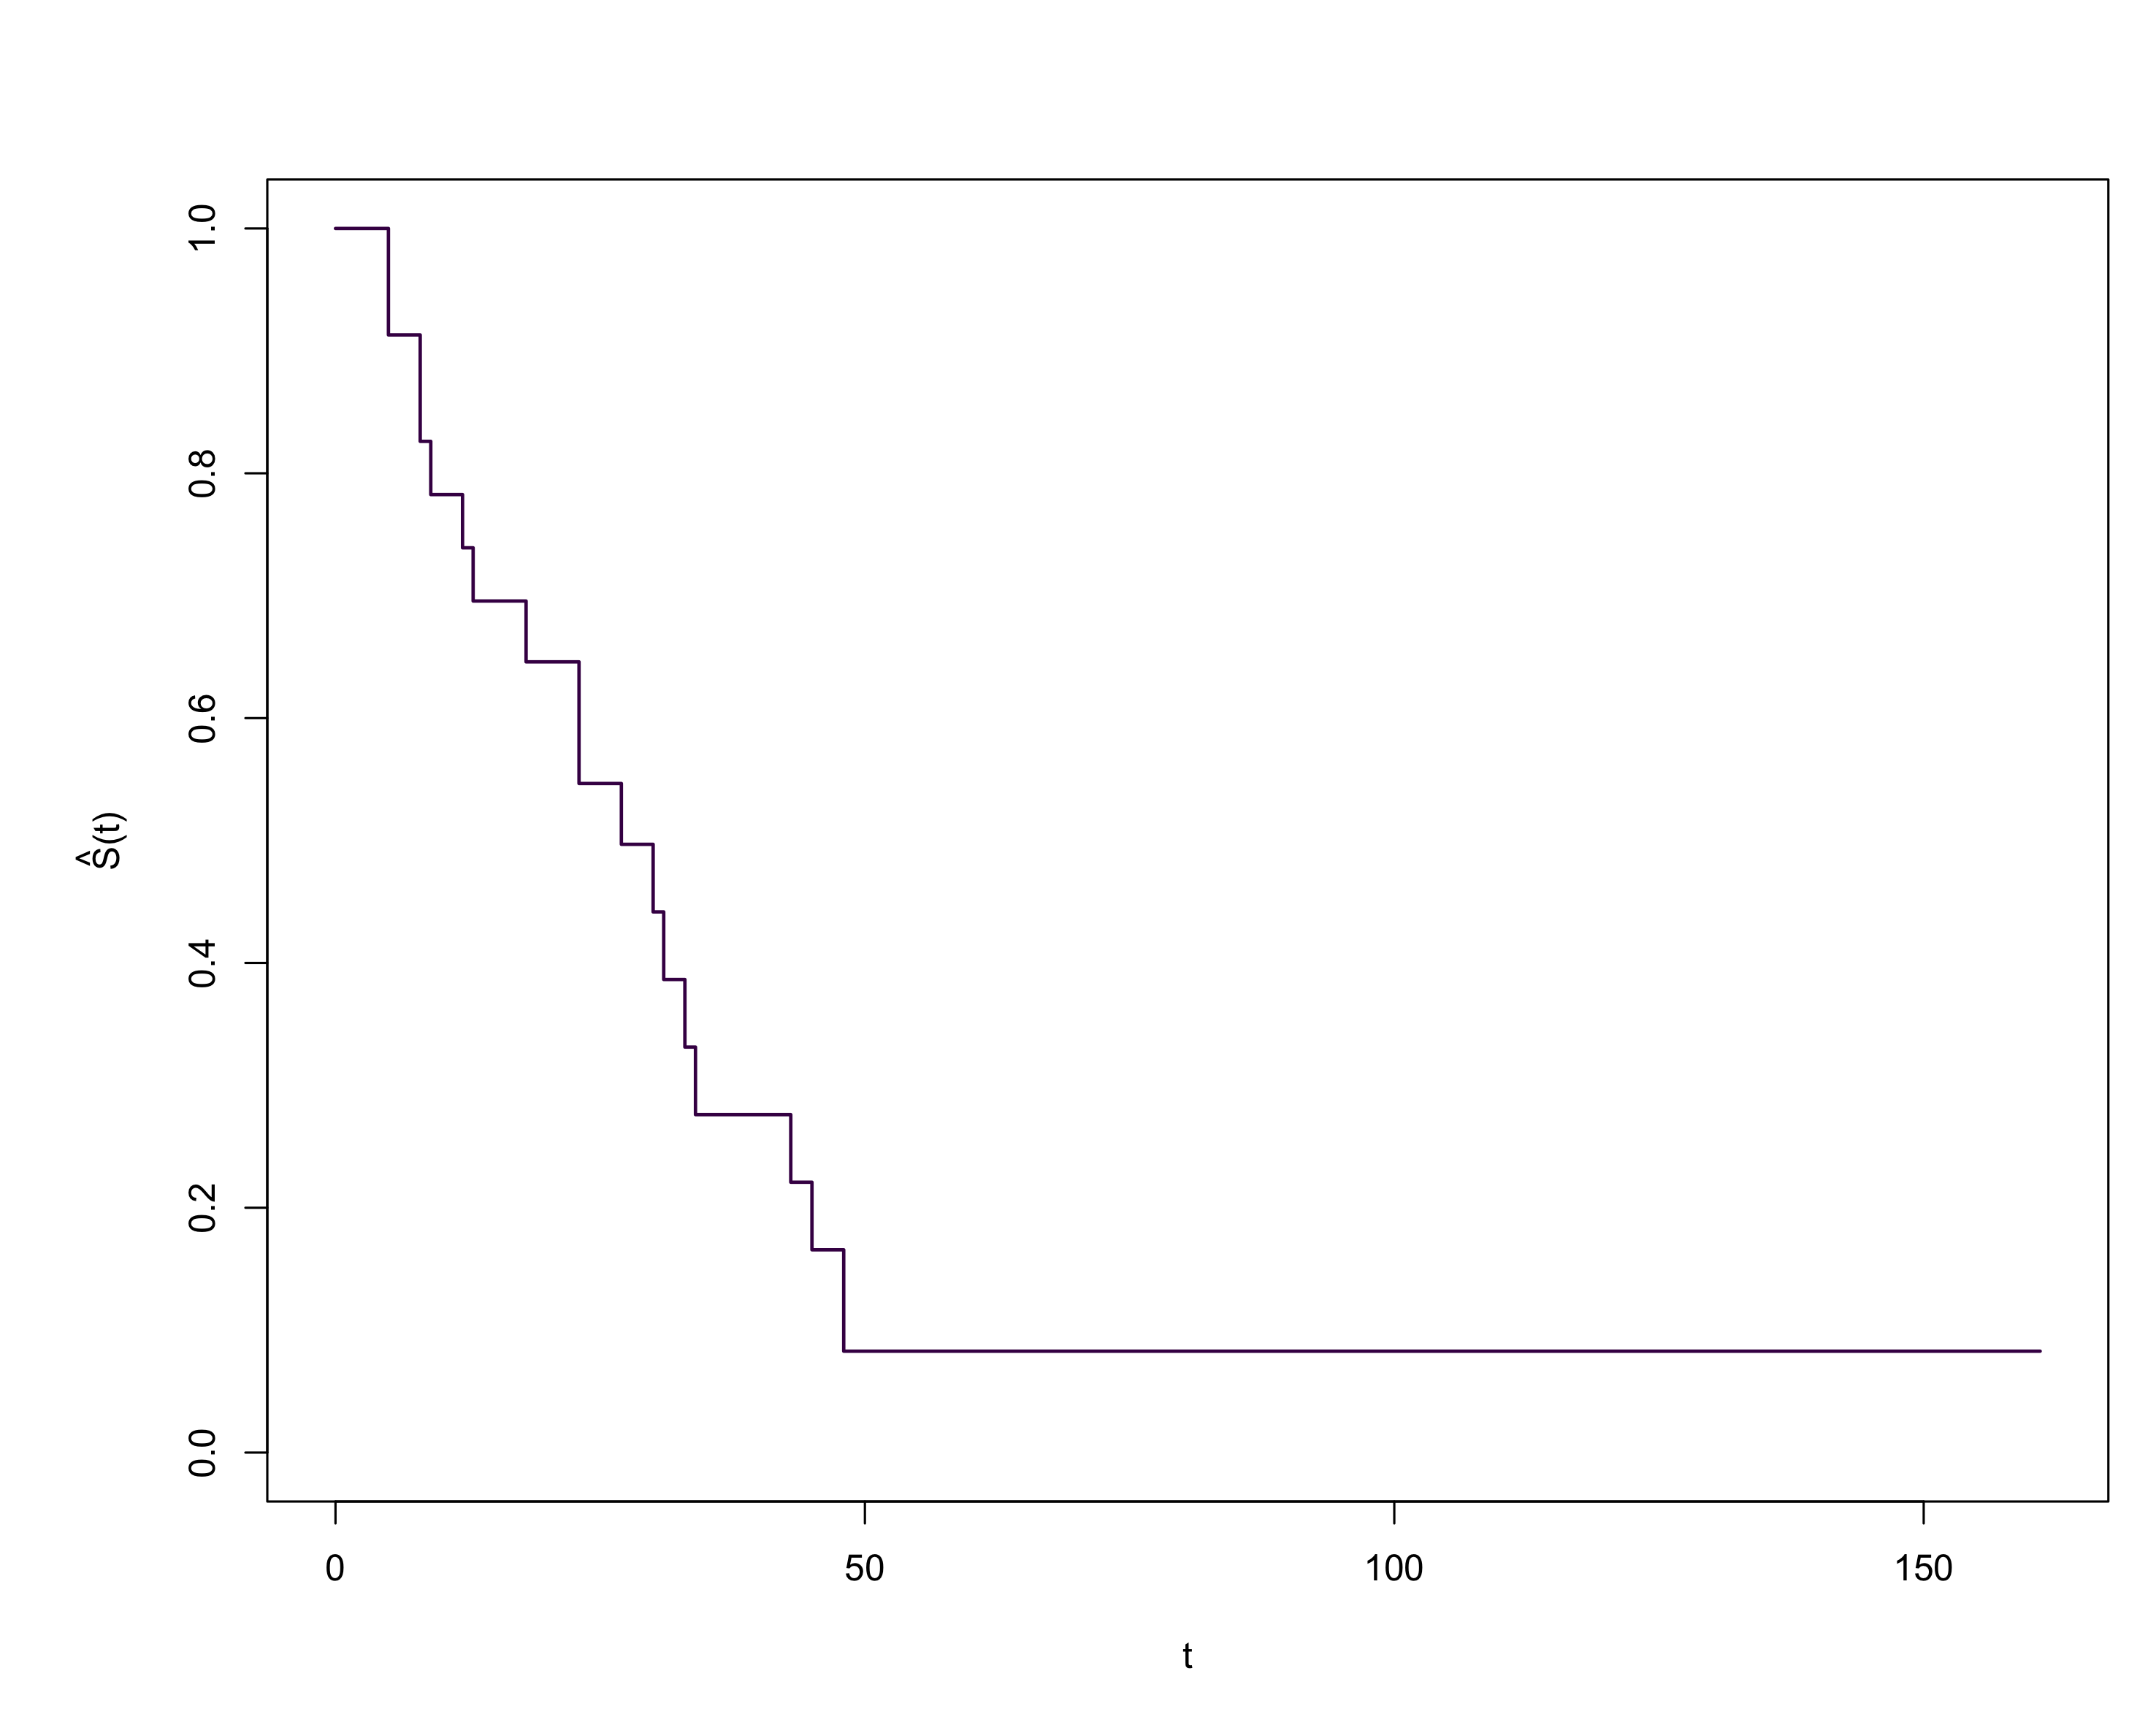
\includegraphics[width=10cm]{km1.png}
\caption{Estimador Kaplan-Meier para los 23 pacientes del estudio.}
\label{fig:km1}
\end{figure}

\begin{figure}
\centering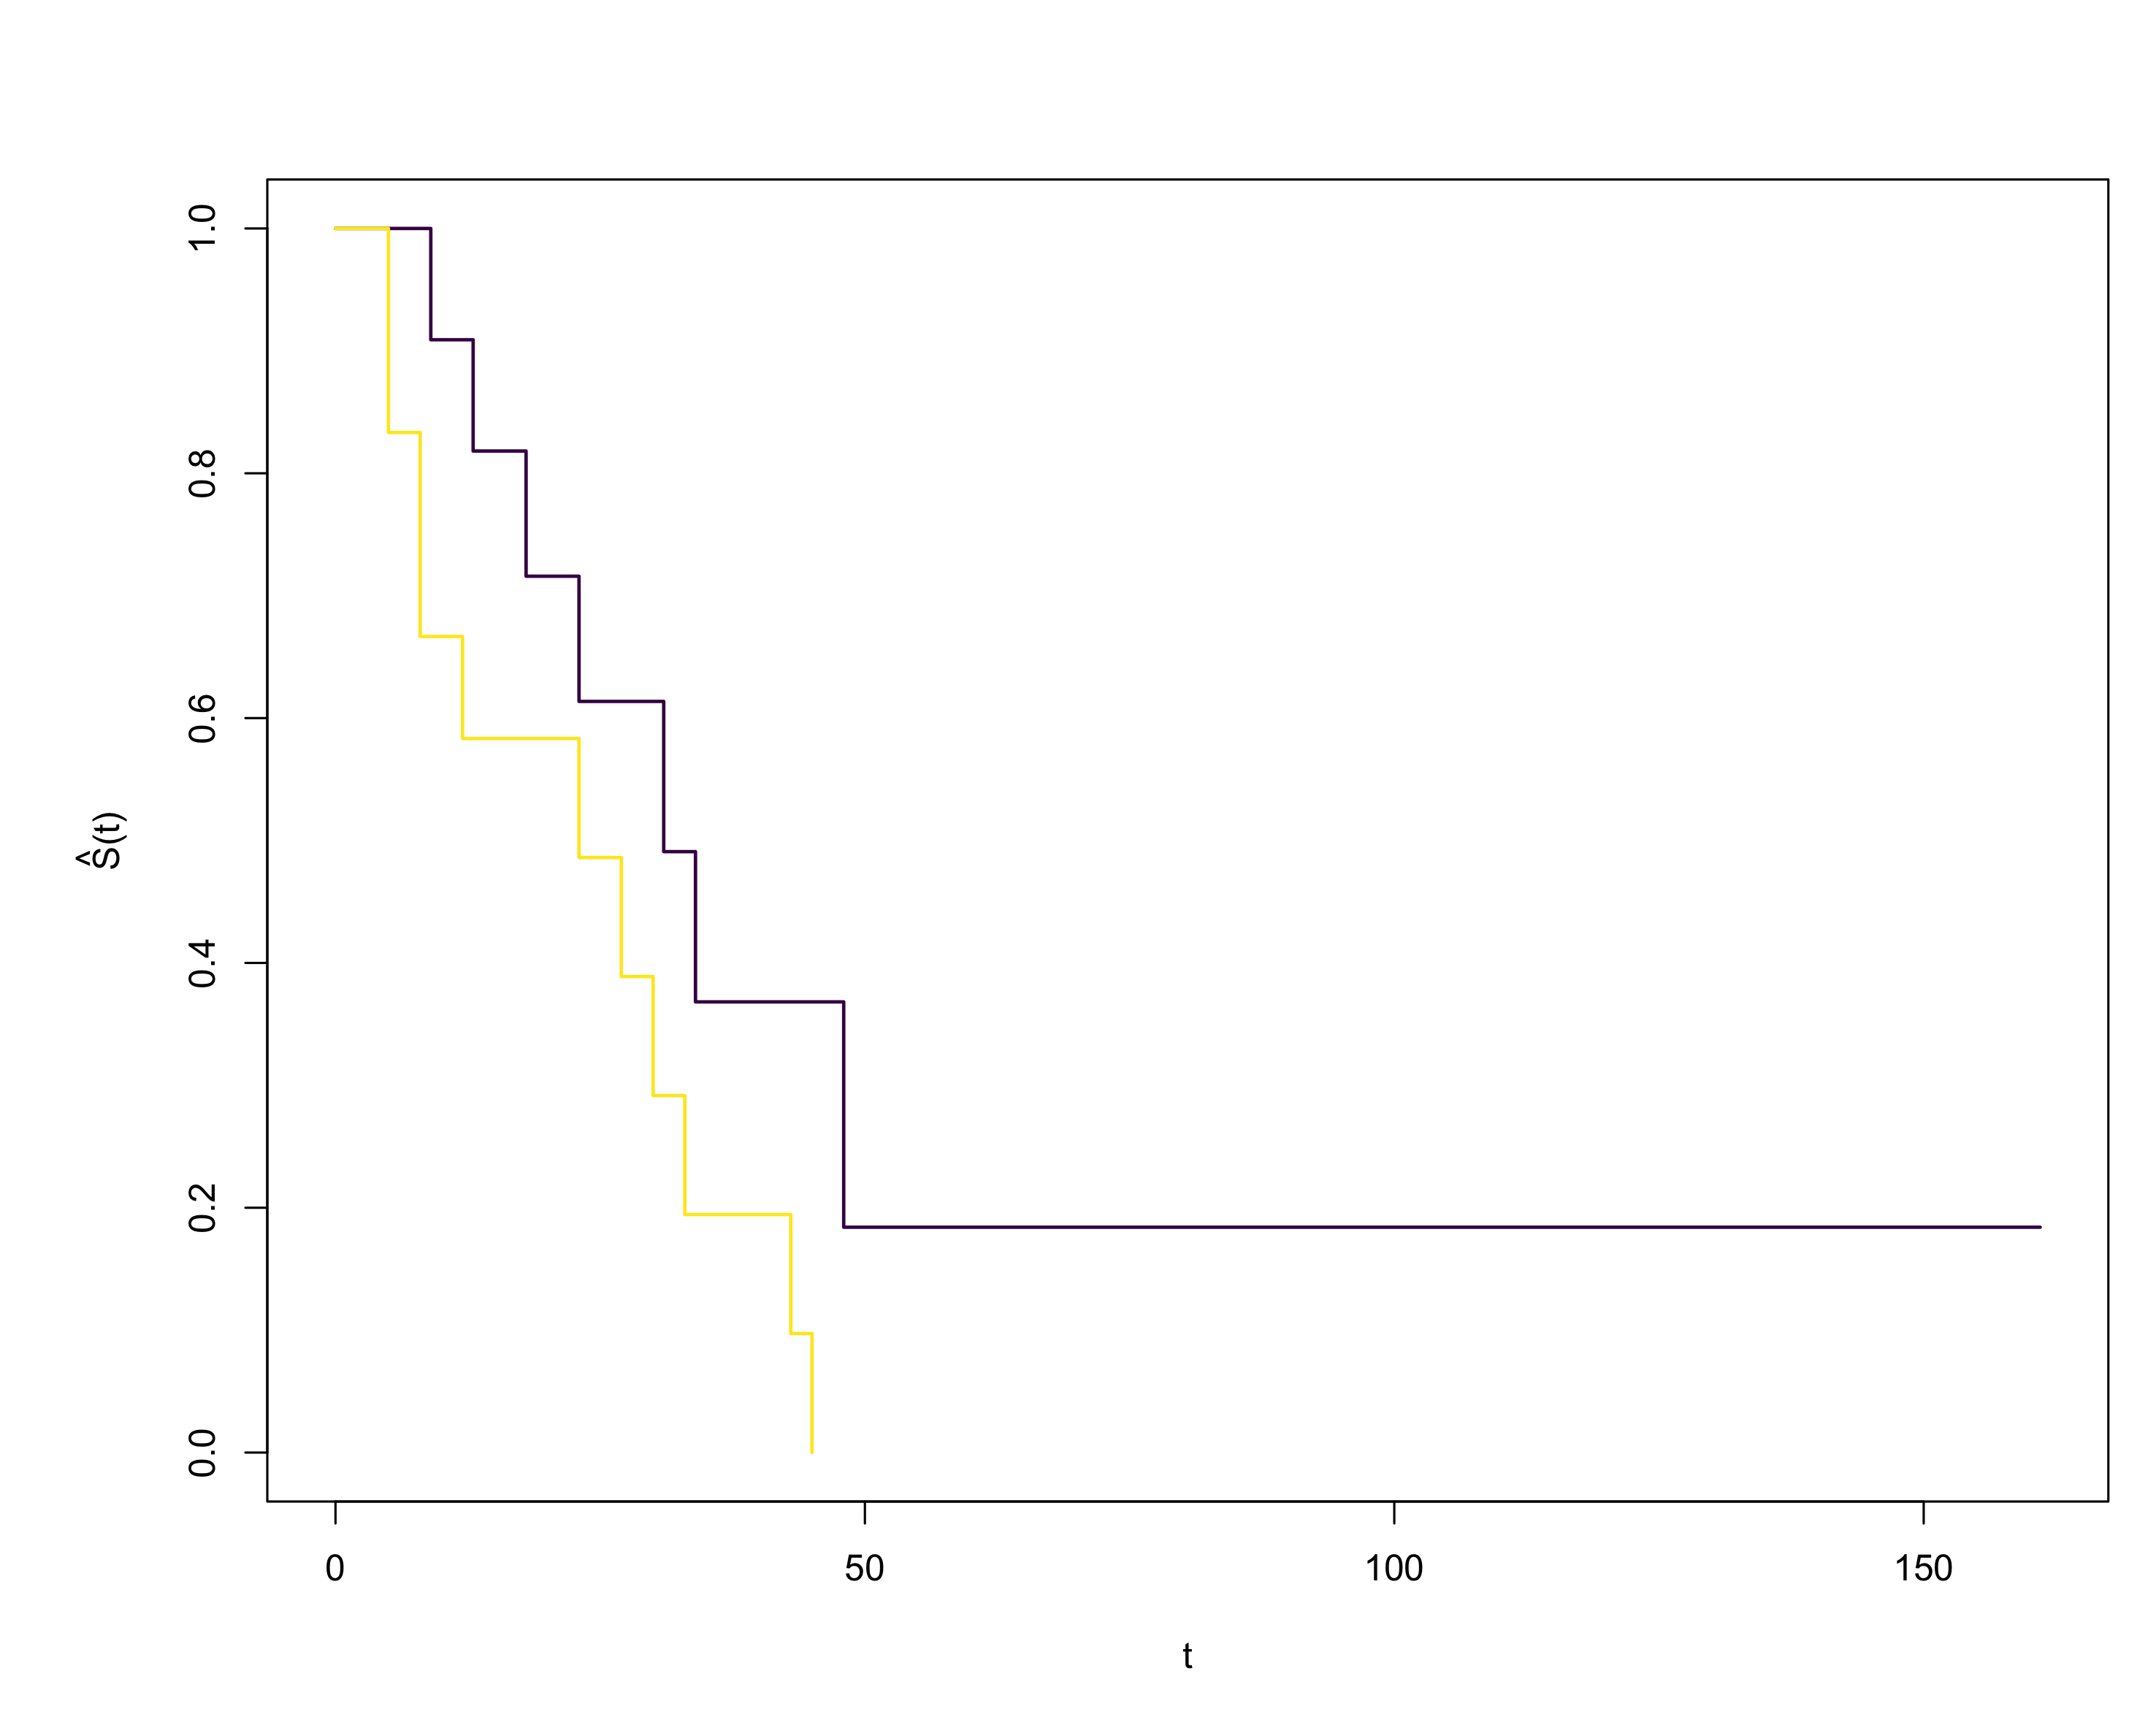
\includegraphics[width=10cm]{km2.png}
\caption{Estimadores Kaplan-Meier para los 11 pacientes que recibieron ciclos adicionales de quimioterapia (verde) y para los 12 que no (naranja).}
\label{fig:km2}
\end{figure}

\subsection{Construcción de la función de verosimilitud}
\label{sec:ver}

El método más utilizado para obtener estimaciones de parámetros poblacionales de interés es el método de máxima verosimilitud. Para utilizar este método es necesario construir la función de verosimilitud, que se puede entender como la distribución conjunta de las observaciones vista como función de los parámetros.\\

En el caso más común cuando se cuenta con una muestra aleatoria $T_1, T_2, \dots, T_n$ de observaciones y todas las observaciones son exactas, la función de verosimilitud es $$\mathcal{L}(\theta) = \prod_{i = 1}^n f(t_i|\theta).$$ Es de interés ahora construir la función de verosimilitud cuando algunos datos aportan información parcial, es decir, cuando hay observaciones censuradas y/o truncadas.\\

Siguiendo las ideas presentadas en \cite{klein}, pensemos en la información parcial que aportan las observaciones para construir la verosimilitud. La contribución a la verosimilitud según el tipo de información aportada se presenta en la tabla siguiente.\\

\begin{center}
\begin{tabular}{ |c|c|c| } 
 \hline
 Tipo de observación & Información que aporta & Contribución a $\mathcal{L}(\theta)$\\
 \hline
 & & \\
 Exacta & $T_i$ & $f(t_i)$\\
  & & \\
 Censurada por derecha & $T_i > C_i$ & $S(C_i)$\\
  & & \\
 Censurada por izquierda & $T_i < C_i$ & $1-S(C_i)$\\
  & & \\
 Censurada por intervalo & $L_i < T_i \leq R_i$ & $S(L_i)-S(R_i)$\\
  & & \\
 Truncada por izquierda & $T_i \ | \ T_i > U_i$ & $f(t_i)/S(U_i)$ \\
  & & \\
 Truncada por derecha & $T_i \ | \ T_i < V_i$ & $f(t_i)/(1-S(V_i))$ \\
  & & \\
 Truncada por intervalo & $T_i \ | \ U_i < T_i < V_i$ & $f(t_i)/(S(U_i)-S(V_i))$ \\
  & & \\
 \hline
\end{tabular}
\end{center}

Siguiendo esta lógica, las contribuciones anteriores se pueden mezclar para incorporar otros tipos de información parcial. Por ejemplo, si una observación es truncada por la izquierda y censurada por la derecha, entonces la información que aporta es $T_i>C_i \ | \ T_i > U_i$ y su contribución a $\mathcal{L}(\theta)$ es $S(C_i)/S(U_i)$.\\

Con esta idea ya tenemos las herramientas para construir la función de verosimilitud incorporando información parcial proveniente de observaciones censuradas o truncadas.\\

Es muy importante resaltar que las observaciones truncadas y censuradas no son datos faltantes. Éstas aportan información sobre la variable de interés, por lo que no incorporarlas a la función de verosimilitud sería desechar información relevante. Por otro lado, tomar estas observaciones como si fueran datos exactos es incorrecto ya que puede sesgar la inferencia realizada sobre parámetros de interés. Para reforzar este punto, se presenta a continuación un ejemplo artificial creado en R.\\

Supongamos que se tienen tiempos de fallo con una distribución exponencial $T \sim Exp(1/10)$. Simulamos una muestra aleatoria de 10 mil observaciones de $T$. Luego, supongamos que el monitoreo en el estudio finalizó al tiempo $T = 15$, por lo que todos los individuos con un tiempo de fallo mayor a 15 están censurados por la derecha con un tiempo de censura $C = 15$.\\

Cuando trabajamos con observaciones censuradas y truncadas, es necesario saber cuáles de las observaciones son de este tipo. Cuando solamente se tiene censura por la derecha, es común encontrar las observaciones de $T$ acompañadas de una variable indicadora $\delta$, donde $$\delta_i = \begin{cases}
1, & \text{si } t_i \text{ es exacto},\\
0, & \text{si } t_i \text{ es censurado por derecha}
\end{cases}.$$\\

Utilizando esta notación, se tiene que la función de log-verosimilitud para $\lambda$ está dada por $$l(\lambda) = \lambda \sum_{i = 1}^n \delta_i - \lambda \left(\sum_{i: \delta_i = 1} t_i + \sum_{i: \delta_i = 0} C_i\right).$$ A continuación, se presenta una gráfica de las funciones de log-verosimilitud con su respectivo estimador de máxima verosimilitud, en los siguientes tres casos:
\begin{enumerate}
\item $\hat{\lambda}_1$ incorporando la información de censura,
\item $\hat{\lambda}_2$ suponiendo que todos los datos son exactos,
\item $\hat{\lambda}_3$ eliminando los datos censurados.\\
\end{enumerate}

\begin{figure}[H] 
\centering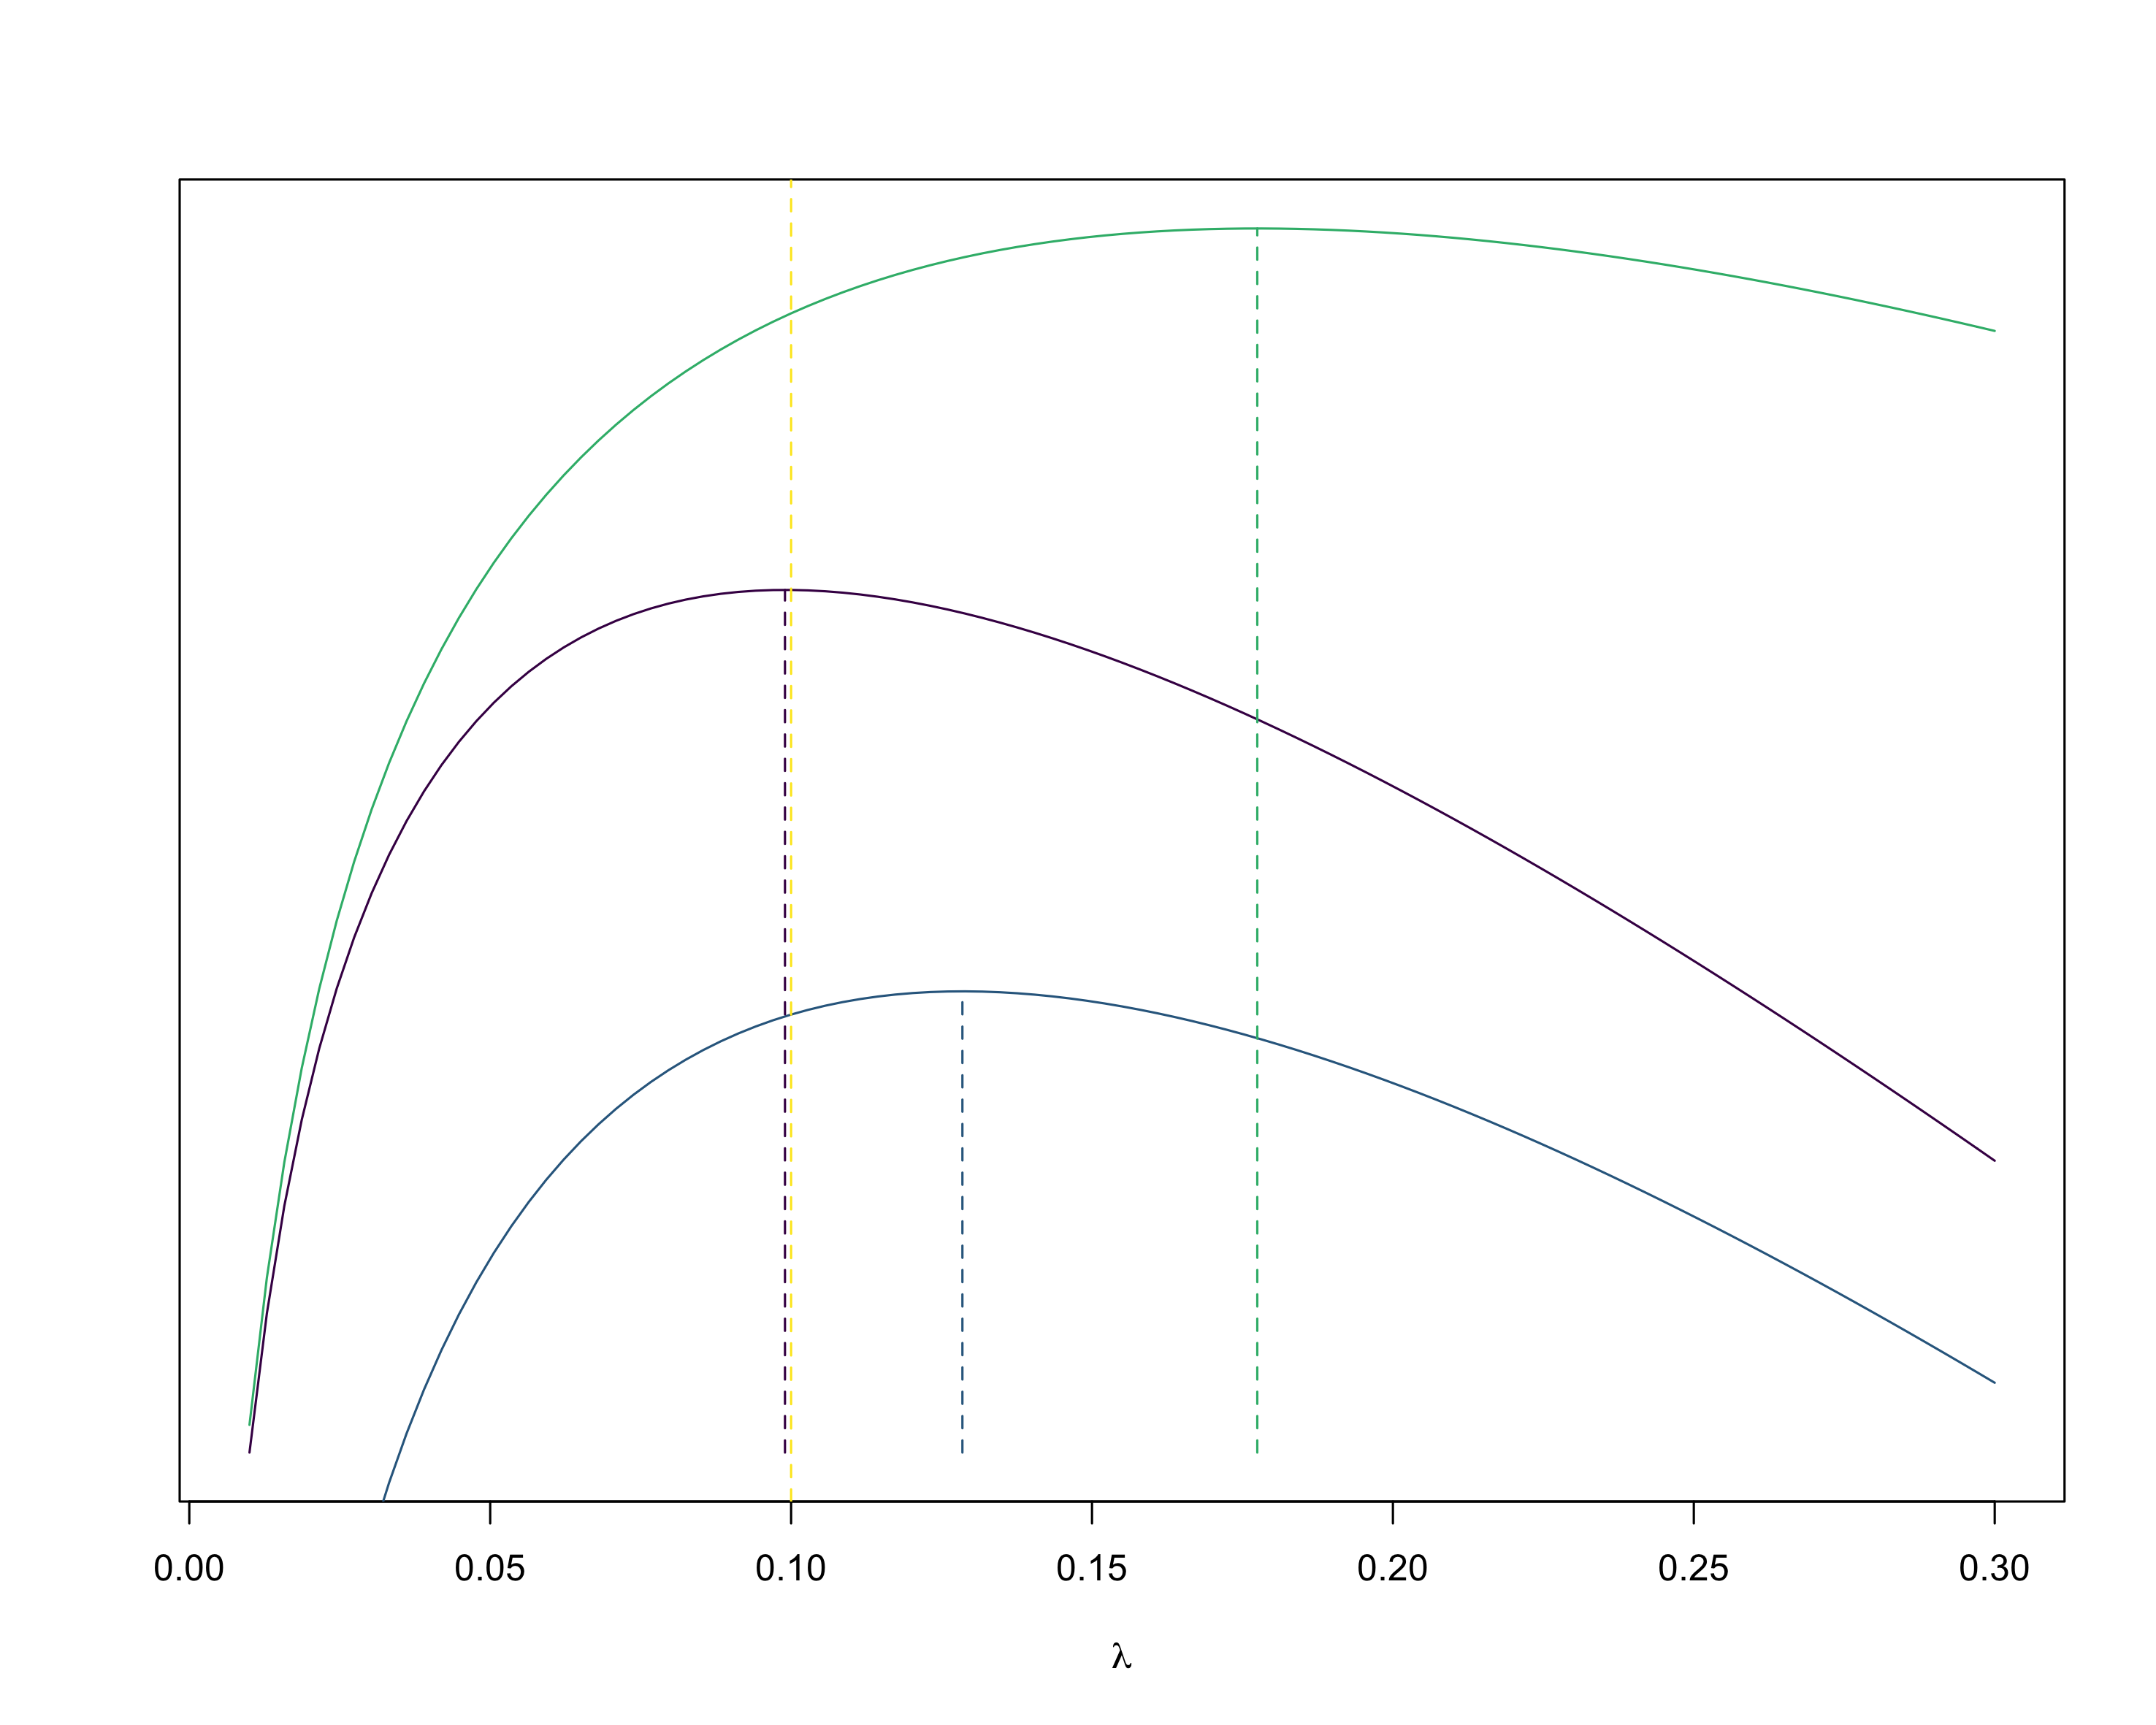
\includegraphics[width=12cm]{likelihood.png}
\caption{$\hat{\lambda}_1$ (azul), $\hat{\lambda}_2$ (verde), $\hat{\lambda}_3$ (naranja) con el valor real $\lambda$ (gris) y las respectivas funciones de log-verosimilitud.}
\label{fig:lik}
\end{figure}

Se puede apreciar claramente en la figura \ref{fig:lik} que el estimador que incorpora la información de censura es el más cercano al valor real. El estimador $\hat{\lambda}_2$ sobrestima el valor real del parámetro ya que se están tomando como exactos los datos censurados por la derecha (recordemos que $E[T] = 1/\lambda$), mientras que el estimador $\hat{\lambda}_3$ está descartando todos los valores $t_i > 15$, por lo que el parámetro también es sobrestimado.\\

El código para reproducir este ejemplo se puede encontrar en el apéndice \ref{ap:lik}.

\subsection{Modelo de regresión de Cox}
\label{seccion_coxph}
En 1972, en el artículo \textit{Regression Models and Life-Tables}, el estadístico inglés David Cox presentó un modelo para describir la función de riesgo de un individuo como función de un vector de variables explicativas y un vector de coeficientes.\\

Para el individuo $j$, sea $z_j\in \mathbb{R}^p$ su vector de covariables. El modelo de Cox consiste en modelar la función de riesgo de este individuo como
\begin{equation} \label{cox_ph}
h_j(t) = h_0(t)e^{z_j^T\beta},
\end{equation}
donde $\beta\in \mathbb{R}^p$ es el vector de coeficientes y $h_0$ es una función de riesgo base, común a todos los individuos, que describe a un hipótetico individuo para el cual $z = 0$.\\

En el caso específico en que $z$ sea una variable indicadora para distinguir un grupo control y un grupo piloto, $h_0$ es la función de riesgo para los individuos en el grupo control y $e^\beta$ es la constante por la cual se multiplica la función de riesgo de los individuos en el grupo piloto.\\

Es común encontrar este modelo en la literatura bajo el nombre de \textbf{modelo de riesgos proporcionales de Cox}, pero este nombre solamente es aplicable a un caso específico de los que se consideran en el artículo original. Específicamente, si se cumple que el vector de covariables no depende del tiempo, entonces se tiene que para dos individuos $i, j$

\begin{align}
\label{eq:prop_haz}
\frac{h_j(t)}{h_i(t)} &= \frac{h_0(t)\exp (z_j^T \beta)}{h_0(t)\exp (z_i^T \beta)} \nonumber \\
&= \exp ((z_j-z_i)^T \beta),
\end{align}
que es una constante como función del tiempo.\\

Además, tomando logaritmo de ambos lados se tiene que
$$\log \left(\frac{h_j(t)}{h_i(t)}\right) = z^{*T} \beta,$$ donde $z^* = z_j-z_i$. Esto es un modelo lineal en los parámetros para el logaritmo de la razón de tasas de riesgo.\\

Es importante hacer énfasis en que el supuesto de proporcionalidad entre las funciones de riesgo se debe cumplir para utilizar el modelo con covariables independientes del tiempo. Sin embargo, el autor señala  \citep{cox} que se puede introducir esta dependencia del tiempo para describir comportamientos distintos a la multiplicación de las tasas de riesgo.\\

Igualmente novedoso fue el método que presentó David Cox para la estimación de los coeficientes sin hacer supuestos sobre la función de riesgo base $h_0$. En el artículo, él se refiere a una \textit{verosimilitud condicional}. En la literatura es común encontrar este mismo método bajo el nombre de \textit{verosimilitud parcial}.\\

Estos nombres se deben a que, según el autor, \textit{"los intervalos de tiempo en que no se presentan fallas no aportan información sobre $\beta$, ya que en estos intervalos bien podría pasar que $h_0$ sea idéntica a cero"} (Cox, 1972). Es por esto que el autor obtiene la función de verosimilitud en los tiempos de falla $\lbrace t_{(i)} \rbrace$, condicionando sobre los individuos en riesgo en ese tiempo, denotados $\mathcal{R}(t_{(i)})$.\\

Cuando no hay empates en los tiempos de falla, la función de verosimilitud parcial es entonces de la forma
$$\mathcal{L}(\beta) = \prod_{i=1}^n \left(\frac{\exp (z_i^T \beta)}{\sum_{l\in \mathcal{R}(t_{(i)})}\exp (z_l^T \beta)}\right).$$ A partir de aquí, se puede derivar la función para obtener el estimador de máxima verosimilitud $\hat{\beta}$.\\

Es importante resaltar que esta forma de la función de verosimilitud se da cuando no hay empate en los tiempos de falla. En teoría, si la variable de interés es continua, que dos eventos se presenten al mismo tiempo es un evento de probabilidad cero. Sin embargo, en la práctica, estos empates se pueden observar debido al redondeo de los tiempos de fallo o a una verdadera naturaleza discreta en la variable de interés. Algunos métodos para lidiar con estos empates son el método marginal, exacto, de Breslow y el de Efron. Una explicación más profunda de estos métodos excede el enfoque de este trabajo. Se recomienda al lector consultar \citet{moore} para una introducción breve a cada uno de ellos.\\

Ahora se presenta una aplicación en R del modelo de riesgos proporcionales, utilizando el conjunto de datos \texttt{aml} introducido en el apartado \ref{sec:truncados}. Utilizaremos este modelo para cuantificar el efecto de los ciclos adicionales de quimioterapia sobre las funciones de riesgo de los pacientes. Primero, transformaremos la variable explicativa en una variable indicadora, haciendo explícitamente grupo base o control a los pacientes que no recibieron ciclos adicionales de tratamiento.\\

Antes de ajustar el modelo, debemos checar que se cumple la hipótesis de riesgos proporcionales. Para esto, denotemos $h_0$ a la función de riesgo del grupo control y $h_1$ a la del grupo piloto y $S_0$, $S_1$ sus respectivas funciones de supervivencia. Bajo el supuesto de riesgos proporcionales, tenemos que $h_1(t) = h_0(t) e^\beta.$ Utilizando las relaciones entre la función de riesgo y la función de supervivencia introducidas en la sección \ref{analisis_sup}, se sigue que $S_1(t) = S_0(t) ^ {\exp (\beta)}.$ Ahora, tomando logaritmo dos veces y multiplicando por -1 de cada lado, obtenemos lo siguiente:

\begin{align*}
S_1(t) = S_0(t) ^ {\exp (\beta)} &\implies \log (S_1(t)) = e^\beta \ \log (S_0(t))\\
&\implies \log (-\log (S_1(t))) = \beta + \log (-\log (S_0(t))).\\
\end{align*}

Es decir, que si graficamos $\log (-\log (S_1(t)))$ y $\log (-\log (S_0(t)))$ contra $t$ o $\log (t)$, bajo el supuesto de riesgos proporcionales debemos ver dos líneas paralelas, separadas por $\beta$. A continuación se presenta esta gráfica utilizando los estimadores Kaplan-Meier de la sección \ref{sec:truncados}.\\

\begin{figure}[H] 
\centering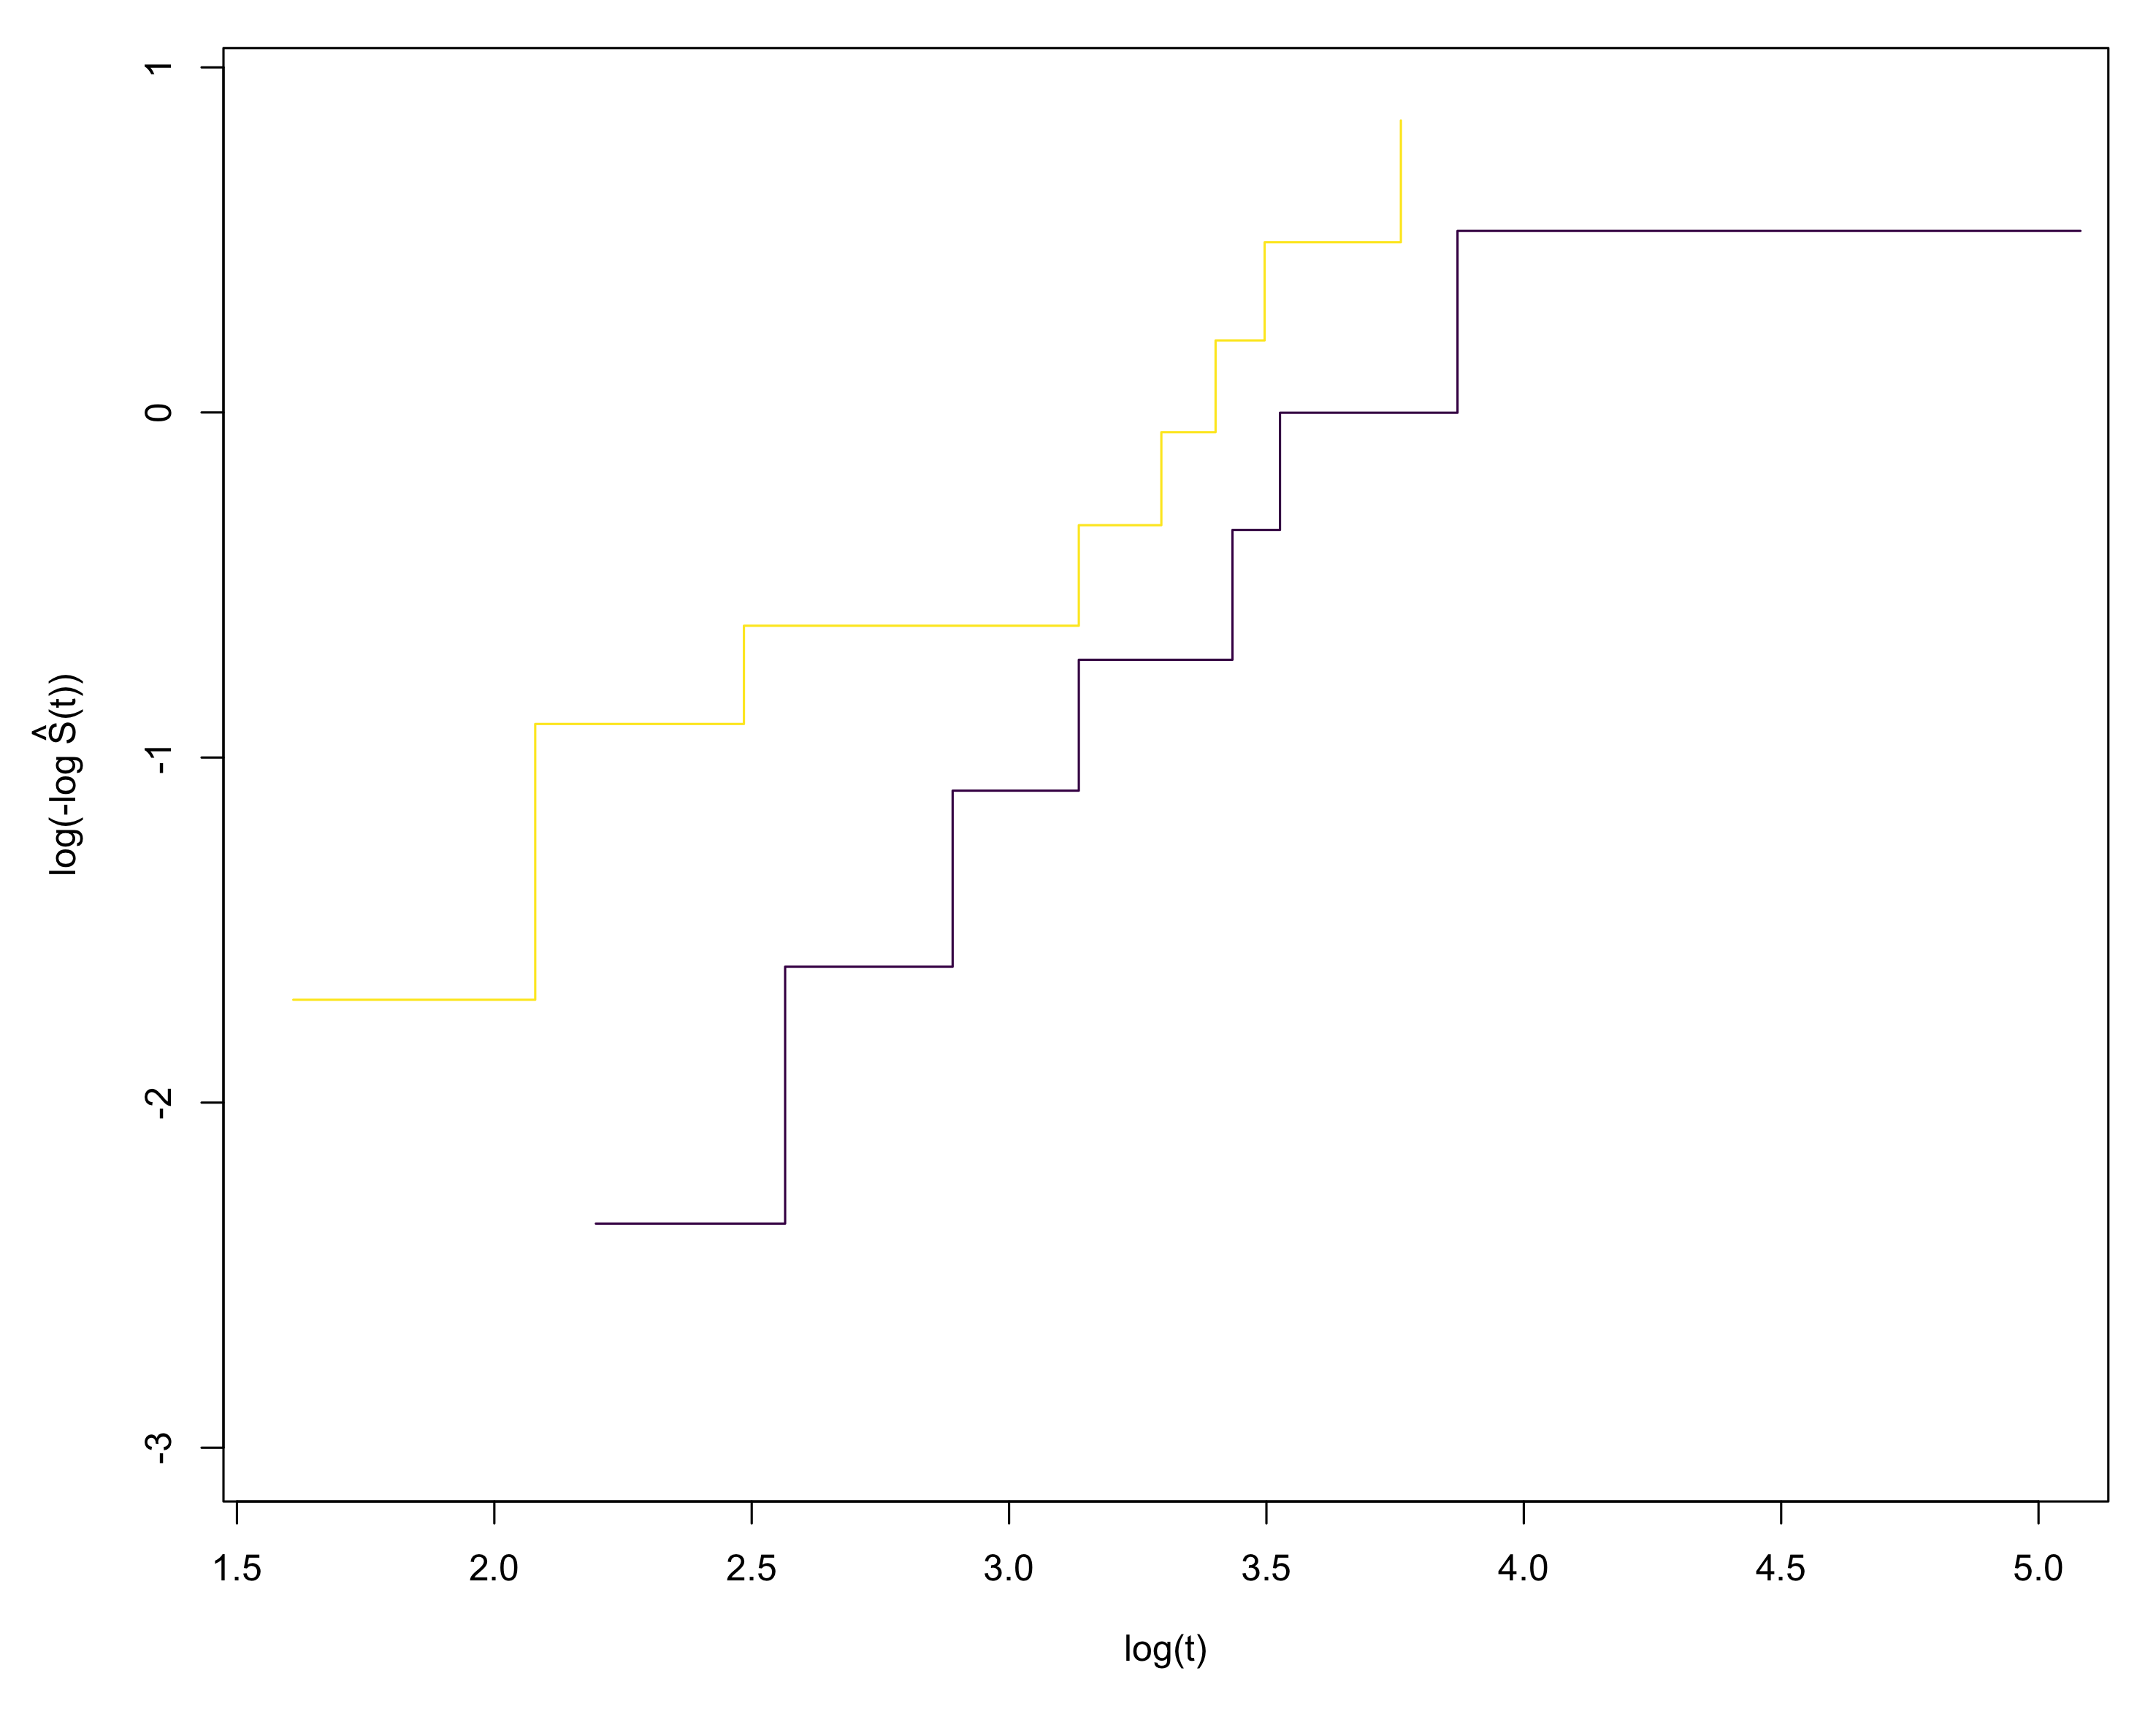
\includegraphics[width=12cm]{prop_haz_km.png}
\caption{Grupo control (naranja) y piloto (verde). No hay evidencia visual para descartar el supuesto de riesgos proporcionales.}
\label{fig:coxph}
\end{figure}

Revisando los datos, podemos ver que tenemos algunos empates en los registros. La documentación de la función \texttt{coxph} señala que estos empates son tratados con el método de Breslow, ya que ``es más preciso y eficiente computacionalmente". Ahora incluimos el código para ajustar el modelo.\\

\begin{lstlisting}
library(survival)
library(tidyverse)

dt_aml <- survival::aml

times <- Surv(dt_aml$time, dt_aml$status)

dt_transform <- dt_aml %>%
  mutate(
    z = case_when(
      x == "Maintained" ~ 1,
      x == "Nonmaintained" ~ 0
    )
  )

model <- coxph(times ~ dt_transform$z)
summary(model)
\end{lstlisting}\leavevmode\newline

El modelo nos arroja una estimación puntual de $\hat{\beta} = -0.9155$. Para interpretar este coeficiente, regresemos a la ecuación \ref{eq:prop_haz}. Tenemos que $$\frac{h_1(t)}{h_0(t)} \approx e^{-0.9155} = 0.4003,$$ es decir, que la tasa de riesgo para el grupo control es aproximadamente 2.5 veces mayor que la del grupo piloto. Este resultado parece indicar una disminución considerable en la tasa de riesgo para los pacientes que reciben ciclos adicionales de quimioterapia. Se aconseja al lector consultar los resultados completos del modelo con el comando \texttt{summary(model)} ya que también cuenta con un intervalo de confianza y un valor p para el coeficiente en cuestión, además de diversas pruebas estadísticas sobre la función de verosimilitud parcial.\\

Un mayor estudio de este modelo excede los objetivos del presente trabajo. Sin embargo, se recomienda al lector dirigirse al artículo original para consultar más detalles y poder leer lo que se considera un clásico del análisis de supervivencia. Para mayor información sobre pruebas de hipótesis para los coeficientes o la verosimilitud parcial, se recomienda consultar \citet{klein}. Si lo que interesa es la implementación en R, \citet{moore} es una buena referencia en opinión de quien escribe.

\newpage

\section{Simulación de variables aleatorias}
\label{simulacion}

La simulación de variables aleatorias se basa en la posibilidad de generar observaciones de una distribución uniforme en el intervalo $(0, 1)$. Estas observaciones se pueden utilizar para simular distribuciones específicas por medio de métodos como el de la transformada inversa o métodos de aceptación y rechazo. En este capítulo se presentan la construcción y las principales características de dichos métodos.\\

Posteriormente, en la sección \ref{sec_cadenas} se presentan métodos más avanzados de simulación, sin embargo, es importante entender los algoritmos aquí presentados ya que forman la base de los que se utilizarán más adelante.

\subsection{Método de la transformada inversa}
\label{sec:transformada}

Recordemos que la función de distribución $F$ de una variable aleatoria $X$
\begin{align*}
F: \mathbb{R}&\to [0,1]\\
F(x) &= P\{X \leq x\}\\
\end{align*}
tiene las características siguientes:

\begin{enumerate}
\item $F$ es no decreciente,
\item $F$ es continua por la derecha,
\item $\lim\limits_{x\to +\infty}F(x) = 1$ y $\lim\limits_{x\to -\infty}F(x) = 0$.\\
\end{enumerate}

Se define la inversa generalizada de $F$, denotada $F^{-1}:[0,1]\to \mathbb{R}$, como $$F^{-1}(y) = \inf \{x\in S_X: F(x) \geq y\}.$$ Con esta definición se puede verificar que

\begin{itemize}
\item $F^{-1}(F(x)) \leq x$ porque $F$ es no decreciente,
\item $F(F^{-1}(y)) \geq y$ por la definición de $F^{-1}$ y
\item $F^{-1}$ es no decreciente.\\
\end{itemize}

Más aún, si $F$ es estrictamente creciente se tiene que $F^{-1}(F(x)) = x$ y si $F$ es continua se cumple $F(F^{-1}(y)) = y$, por lo que $F^{-1}$ define la inversa de $F$ en el sentido usual si $F$ es continua y monótona estricta.\\

\begin{theorem}[Método de la transformación inversa]
Sea $F$ una función de distribución, $F^{-1}$ su inversa generalizada y sea $U\sim U(0,1)$. Entonces la variable aleatoria $X$ definida como $X = F^{-1}(U)$ tiene función de distribución $F$.\\
\end{theorem}

\begin{proof}
Sea $x\in \mathbb{R}$ fija. Se quiere probar la contención de los eventos $$\{U<F(x)\}\subseteq\{F^{-1}(U)\leq x\}\subseteq\{U\leq F(x)\}.$$ Sea $u$ una observación de la variable aleatoria $U$.

$$u<F(x) \implies F^{-1}(u) \leq F^{-1}(F(x)) \leq x$$
$\therefore \hspace{2pt} \{U<F(x)\} \subseteq\{F^{-1}(U)\leq x\}$ y


$$F^{-1}(u)\leq x \implies u\leq F(F^{-1}(u))\leq F(x)$$
$\therefore \hspace{2pt} \{F^{-1}(U)\leq x\}\subseteq \{U \leq F(x)\}$.\\

De esta forma, se tiene que 
\begin{align*}
P\{U\leq F(x)\} = P\{U<F(x)\} &\leq P\{F^{-1}(U)\leq x\} \leq P\{U \leq F(x)\}\\
\implies F(x) = P\{U \leq F(x)\} &= P\{F^{-1}(U)\leq x\} = P\{X\leq x\}\\
\implies P\{X \leq x\} &= F(x),\\
\end{align*}

con lo que se concluye que $F$ es la función de distribución de $X$.\\
\end{proof}

Con el resultado anterior podemos crear un algoritmo para simular observaciones de una variable aleatoria $X\sim F$.

\begin{enumerate}
\item Calcular $F^{-1}$, la inversa generalizada de $F$.
\item Simular observaciones de $U\sim U(0,1)$.
\item Evaluar $X=F^{-1}(U)$.\\ 
\end{enumerate}

Para ilustrar lo anterior, tomemos como ejemplo la distribución exponencial. $X\sim Exp(\lambda)$ tiene función de densidad dada por $f(x) = \lambda e^{-\lambda x} \mathbb{I}_{(0,\infty)}(x)$ y función de distribución dada por $F(x) = 1-e^{-\lambda x}\mathbb{I}_{(0,\infty)}(x)$. Esta función de distribución es continua y estrictamente creciente en $S_X=[0, \infty)$, por lo que su inversa generalizada corresponde a la inversa en el sentido usual. La inversa de $F$ es $$F^{-1}(y) = -\frac{1}{\lambda}\log (1-y)$$ con $Dom(F^{-1}) = [0, 1)$.\\

A continuación se muestra un ejemplo de la simulación de $F$ para $\lambda = 1/2$, junto con la función de densidad en la fiugra \ref{fig:transformada_inversa}.\\

\begin{lstlisting}
f <- function(x, lambda) lambda * exp(-lambda * x)

dist_inv <- function(y, lambda) -(1/lambda) * log(1-y)

set.seed(42)
nsim <- 10e4
lambda <- 0.5

u <- runif(nsim)

x <- dist_inv(u, lambda)
\end{lstlisting}

\begin{figure} 
\centering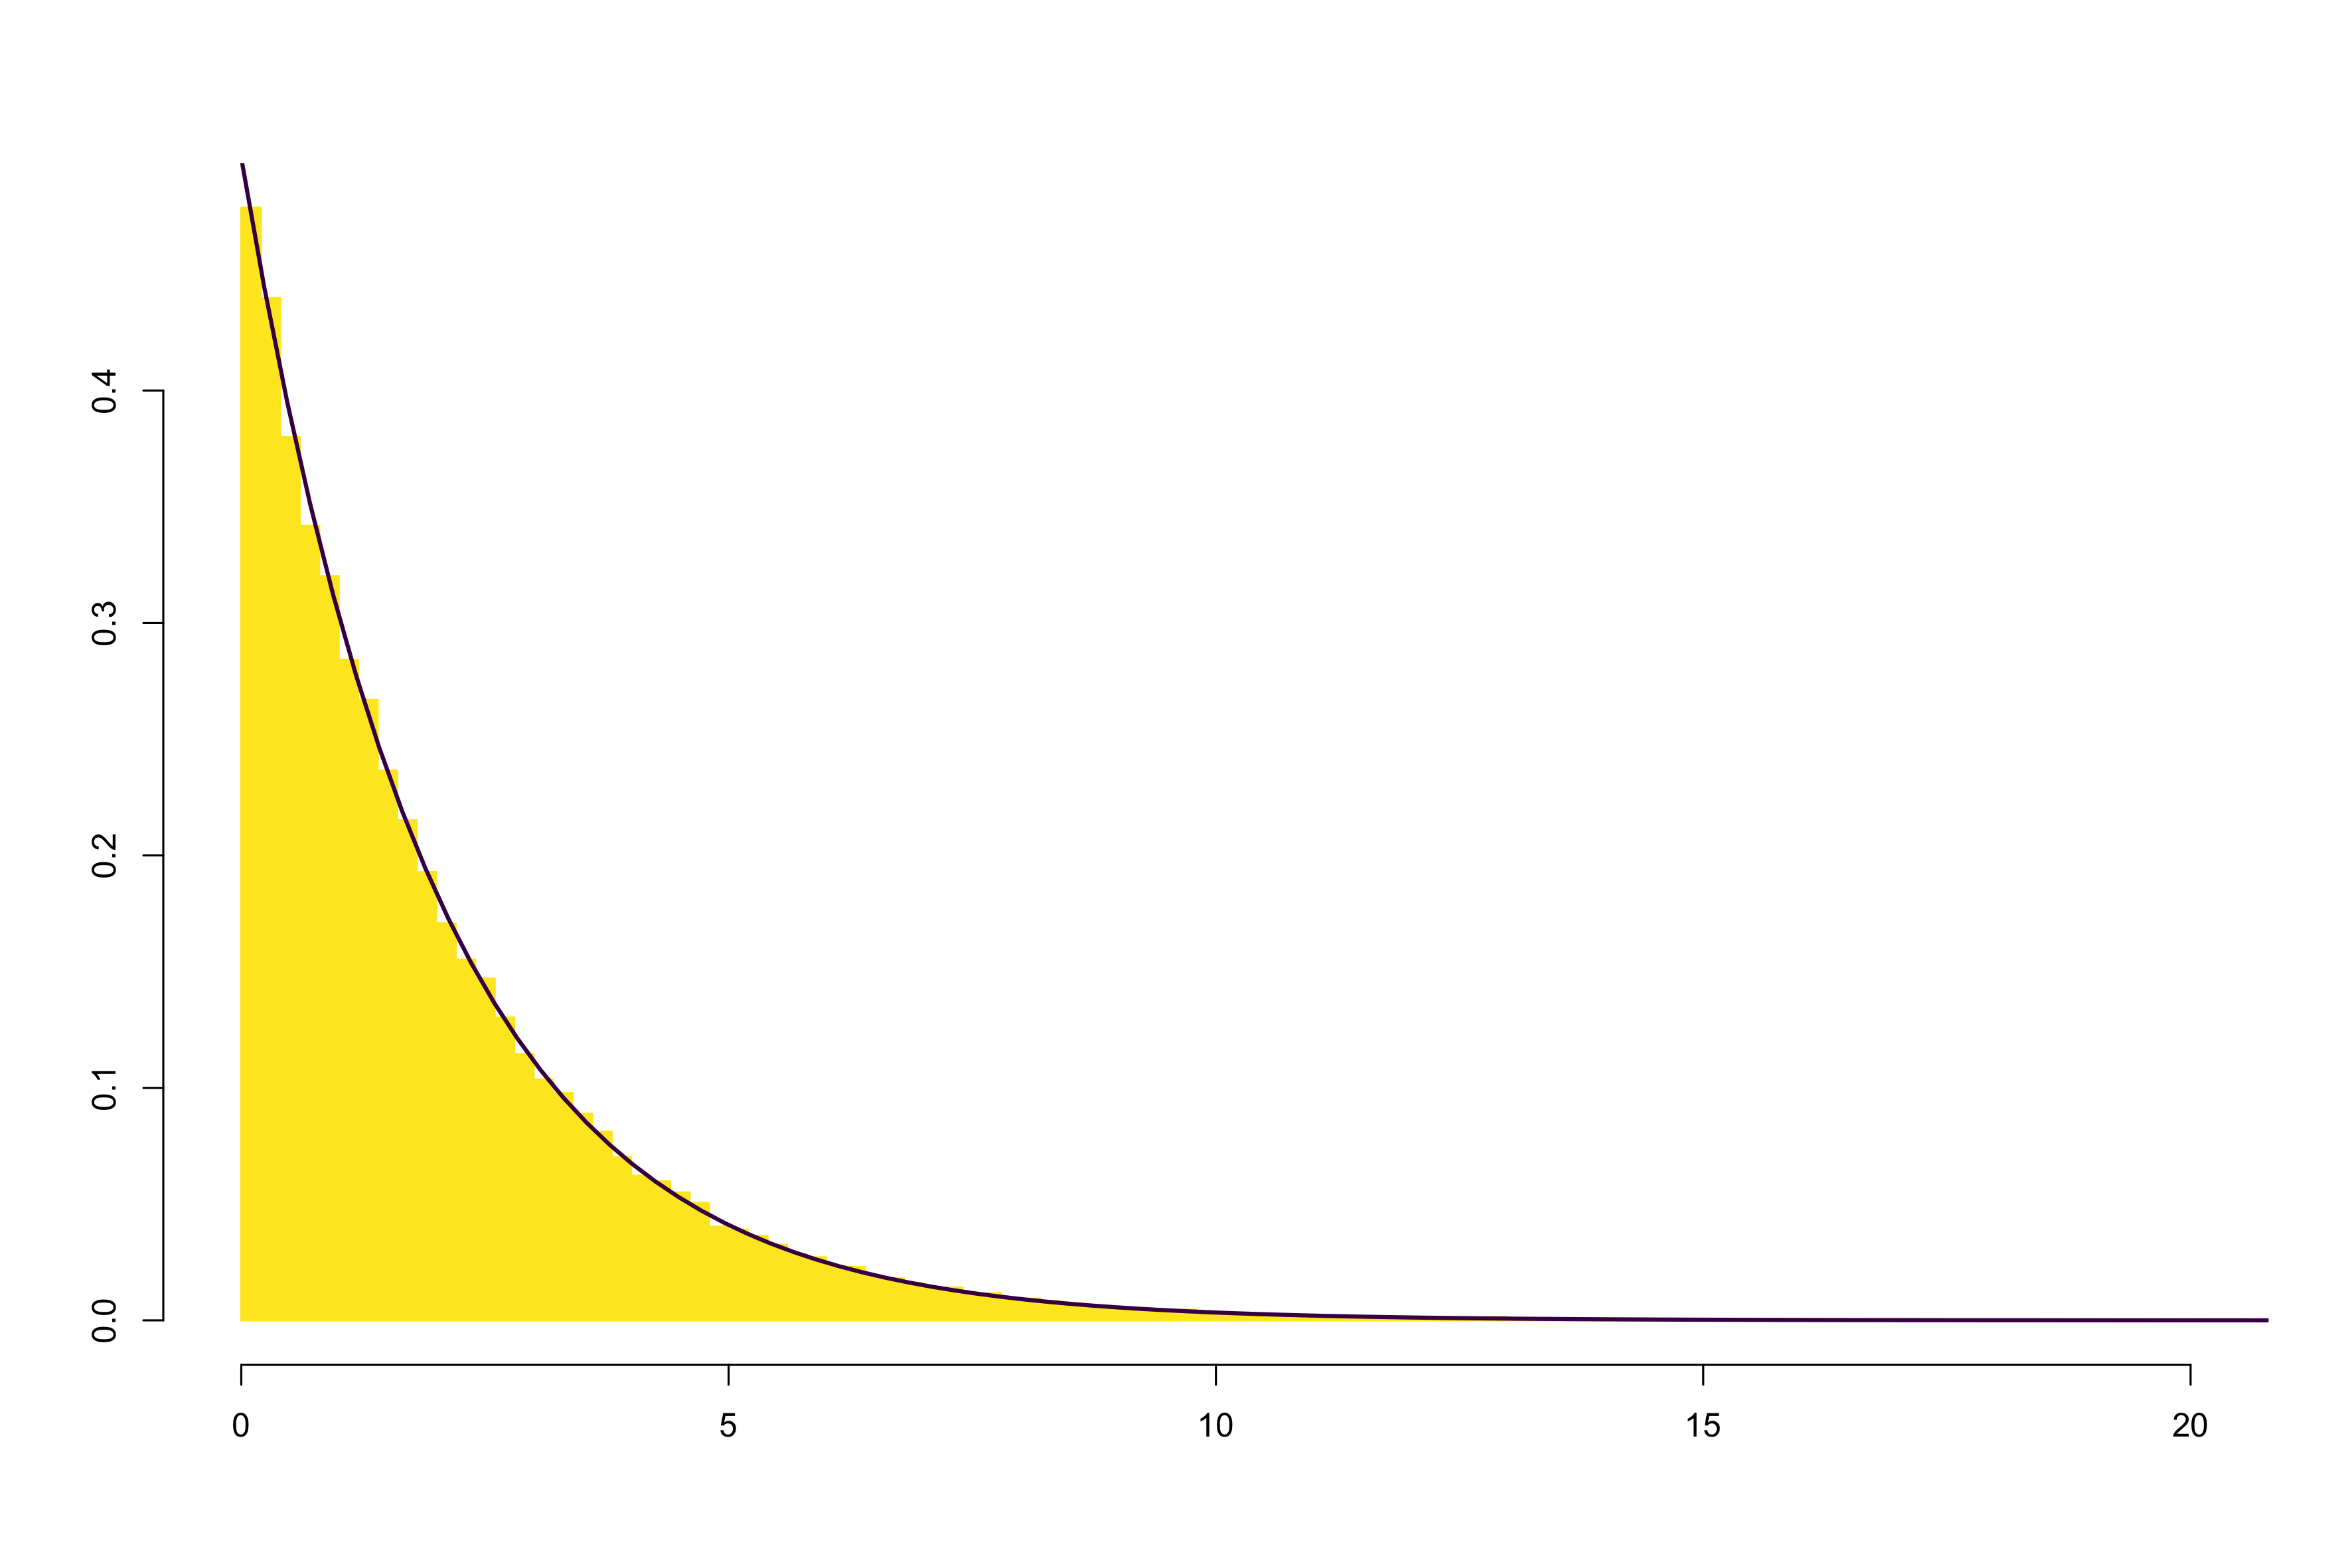
\includegraphics[width=10cm]{transformada_inversa.png}
\caption{Histograma de las simulaciones de $f \sim Exp(0.5)$ con la densidad real.}
\label{fig:transformada_inversa}
\end{figure}

En \citet{casella} se presenta un algoritmo para simular distribuciones que pueden ser representadas como mezclas.\\

\textbf{Simular distribuciones representadas como mezclas.} Supongamos que la variable aleatoria $X$ puede ser representada como una mezcla, esto es

\begin{equation}
f(x) = \int_{S_Y} f(x|y)g(y)dy.
\label{mezcla_sim}
\end{equation}

Idealmente, $g(y)$ y $f(x|y)$ deben ser densidades fáciles de simular, por ejemplo, con el método de la transformada inversa. Para simular entonces observaciones de $X$ se utiliza el algoritmo siguiente:

\begin{enumerate}
\item Simular una observación $y$ de $Y\sim g$.\\
\item Simular $X|y \sim f(x|y)$.\\
\item Las observaciones resultantes tienen una distribución dada por la función de densidad \eqref{mezcla_sim}.\\
\end{enumerate}

En las librerías de R base no contamos con una función para simular directamente la distribución $t$ con parámetros de localización y escala. Aprovecharemos su representación como mezcla para crear un algoritmo que nos permita simularla.\\

En \citet{gelman} se menciona que si $X\sim t_\nu (\mu, \sigma^2)$, entonces $X$ puede ser representada como una mezcla tomando 
\begin{align*}
X|Y &\sim \mathcal{N}(\mu , Y)\\
Y &\sim \chi ^{-2}(\nu, \sigma ^2)\\
\end{align*}

o de manera equivalente

\begin{align*}
X|Y &\sim \mathcal{N}(\mu , Y)\\
\frac{\nu\sigma ^2}{Y} &\sim \chi ^2_{\nu}.\\
\end{align*}

Las observaciones de la distribución Normal se obtienen con la función \texttt{rnorm}. La documentación de esta función, accesible con el comando \texttt{?rnorm} indica que esta simulación se hace utilizando el método de la transformada inversa.\\

La simulación de la distribución $\chi^2$ se hace utilizando la función \texttt{rchisq} en R. En la documentación de esta función podemos ver que las observaciones se obtienen simulando una distribución Gamma, la cual se simula con un método de aceptación y rechazo como los que se presentan en la sección \ref{aceptacion}.\\

\begin{figure}[H] 
\centering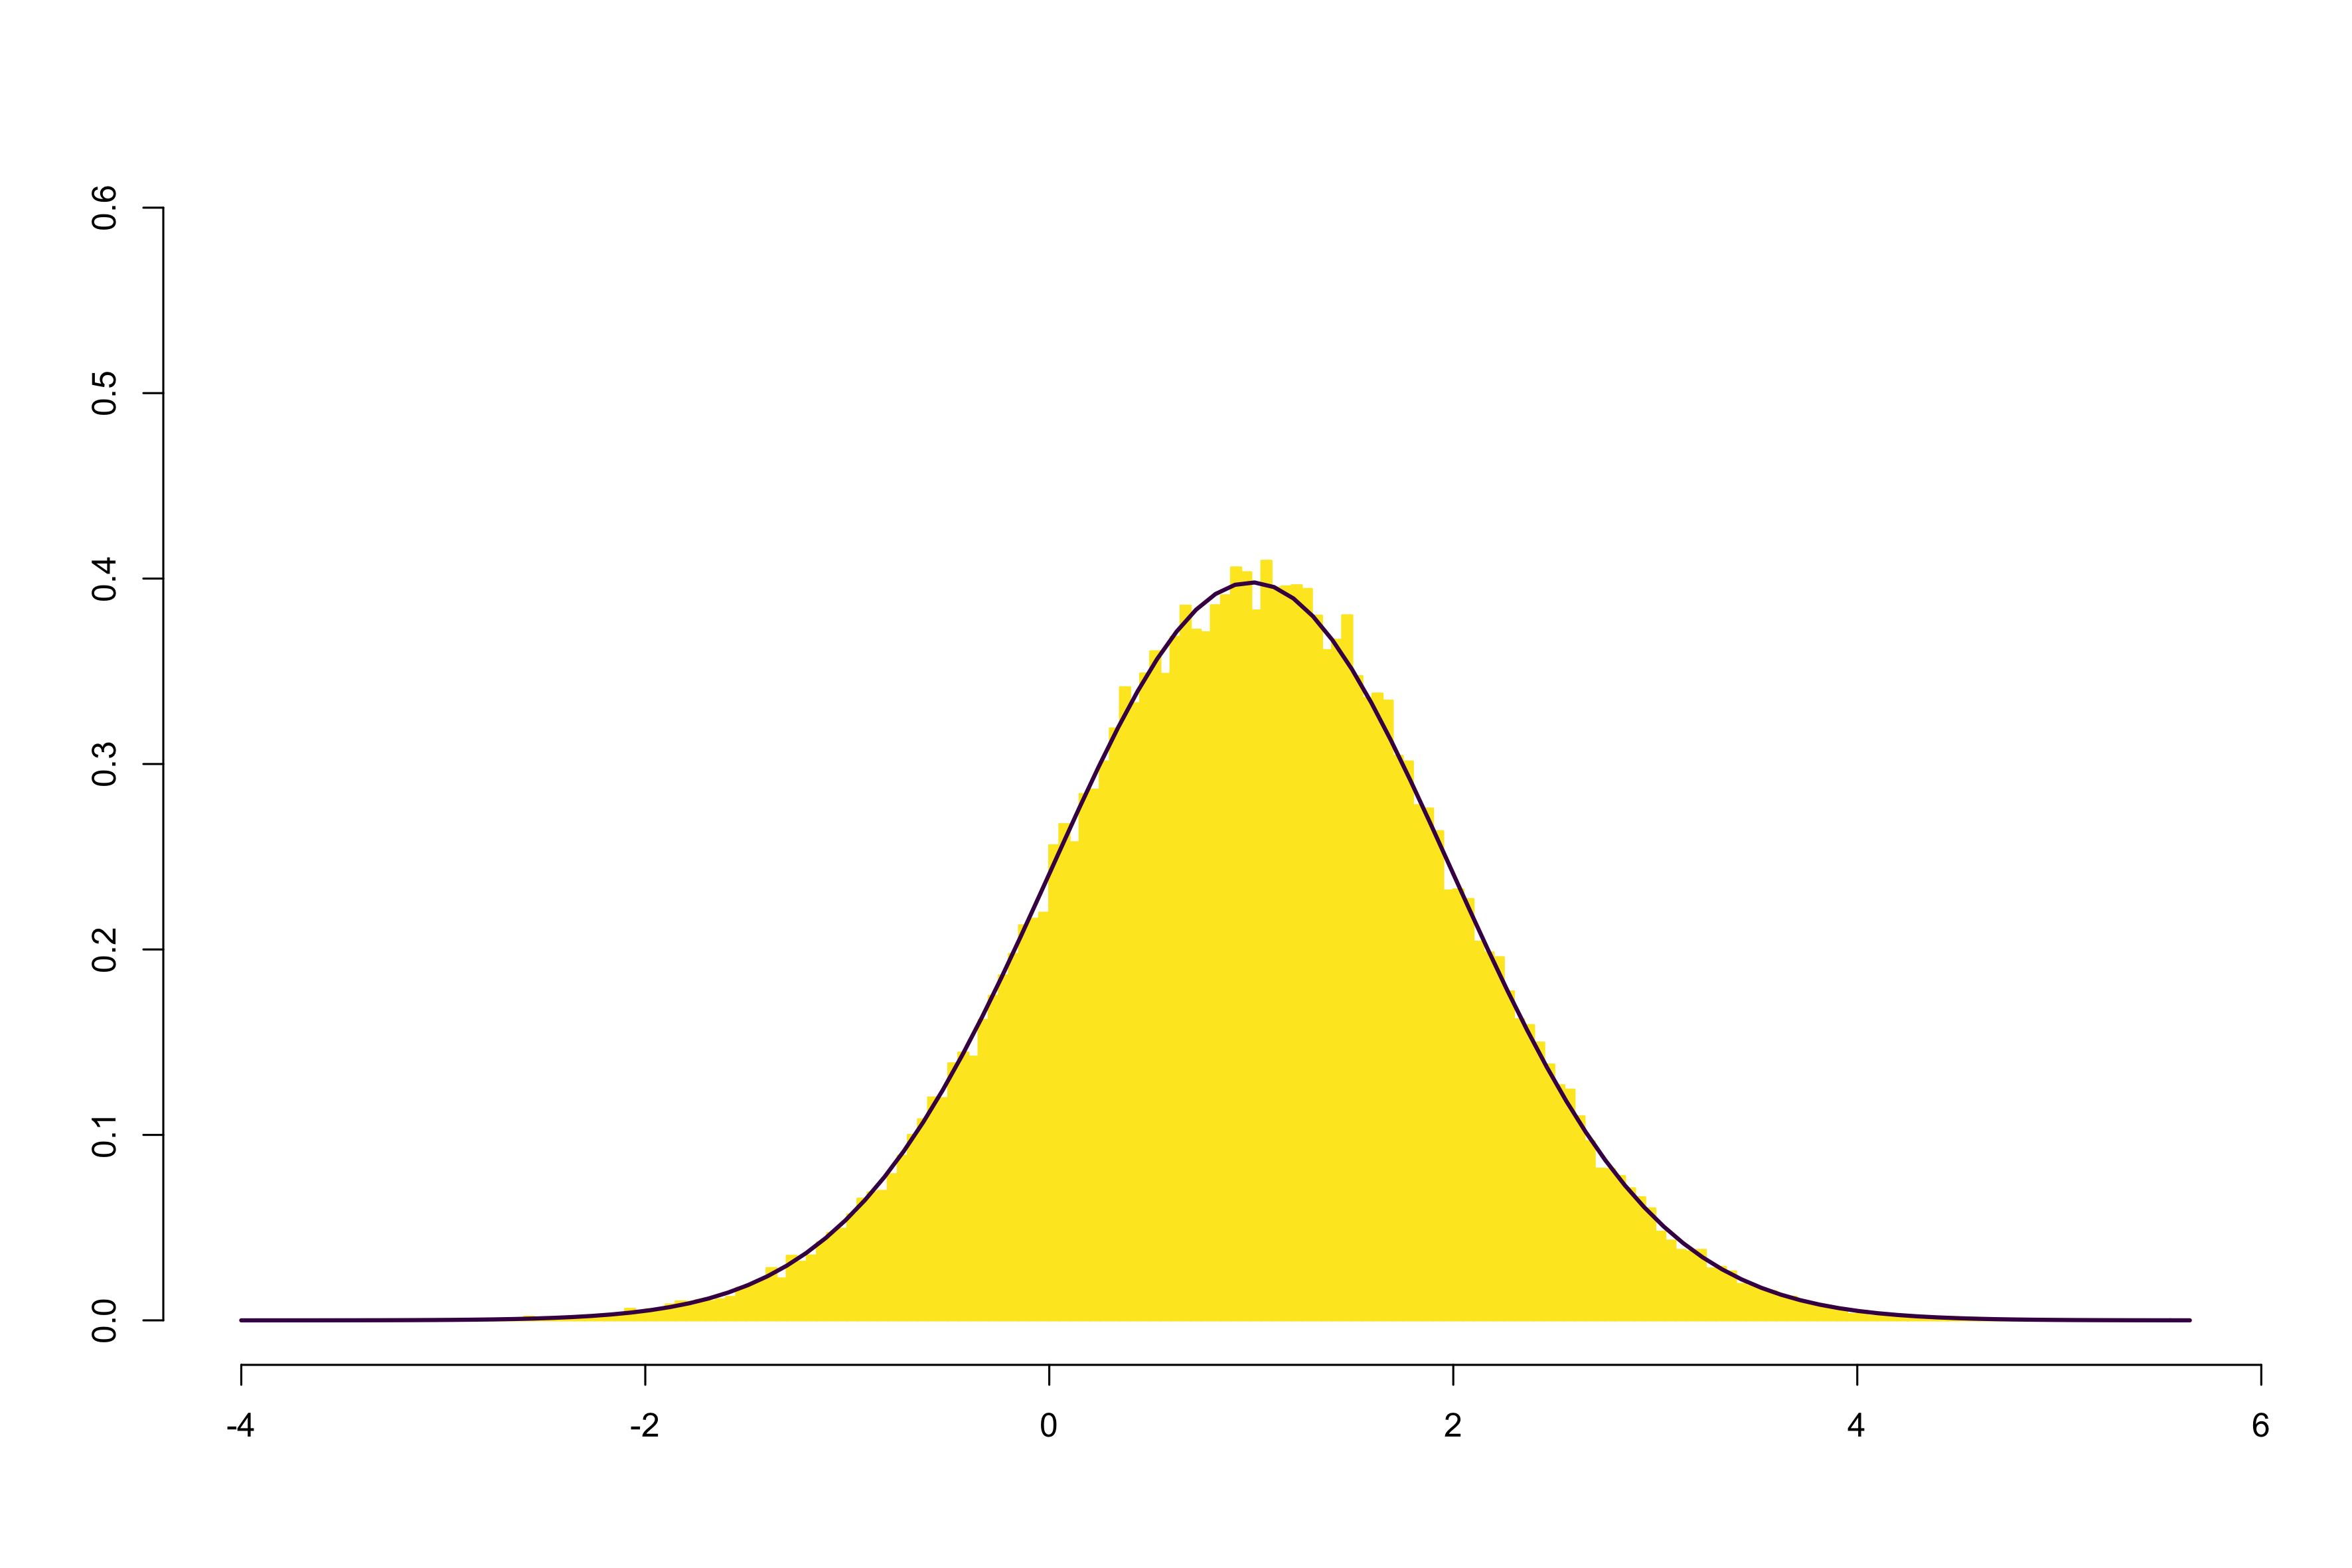
\includegraphics[width=10cm]{sim_mezcla.png}
\caption{Histograma de las simulaciones de $f \sim t_{(100)} (\mu = 1, \sigma = 1)$ con la densidad real.}
\label{fig:t}
\end{figure}

Otro ejemplo de distribuciones generadas por mezclas es el de la distribución Poisson-gamma, denotada como $f \sim Pg(\alpha, \beta, \gamma)$. Se presenta este ejemplo porque la distribución es utilizada en la sección \ref{elmodelo}. La función de probabilidad de una variable aleatoria discreta con distribución Poisson-gamma está dada por
\begin{equation}
\label{eq:poga}
p(x \ | \ \alpha, \beta, \gamma) = \frac{\beta ^ \alpha}{\Gamma (\alpha)}\frac{\Gamma (\alpha + x)}{x!}\frac{\gamma ^ x}{(\beta + \gamma) ^ {\alpha + x}}
\end{equation}
con $S_X = \mathbb{N} \cup \lbrace 0 \rbrace$ y $\alpha, \beta, \gamma \in \mathbb{R}^+$.\\

En \citet{bernardo} se menciona que esta distribución es generada por una mezcla de la forma
$$p(x \ | \ \alpha, \beta, \gamma) = \int_0 ^\infty Po(x \ | \ \gamma \lambda) Ga(\lambda \ | \ \alpha, \beta) \ d\lambda,$$ por lo que podemos utilizar el algoritmo mencionado anteriormente para simular observaciones de $p$.\\

A continuación se presenta el histograma de las simulaciones para $\alpha = 2$, $\beta = 1$ y $\gamma = 5$. Para simular las observaciones de $Ga(\lambda \ | \ \alpha, \beta)$ y $Po(x \ | \ \gamma \lambda)$ utilizamos las funciones \texttt{rgamma} y \texttt{rpois} incluidas en los paquetes de R base.\\

\begin{figure}[H] 
\centering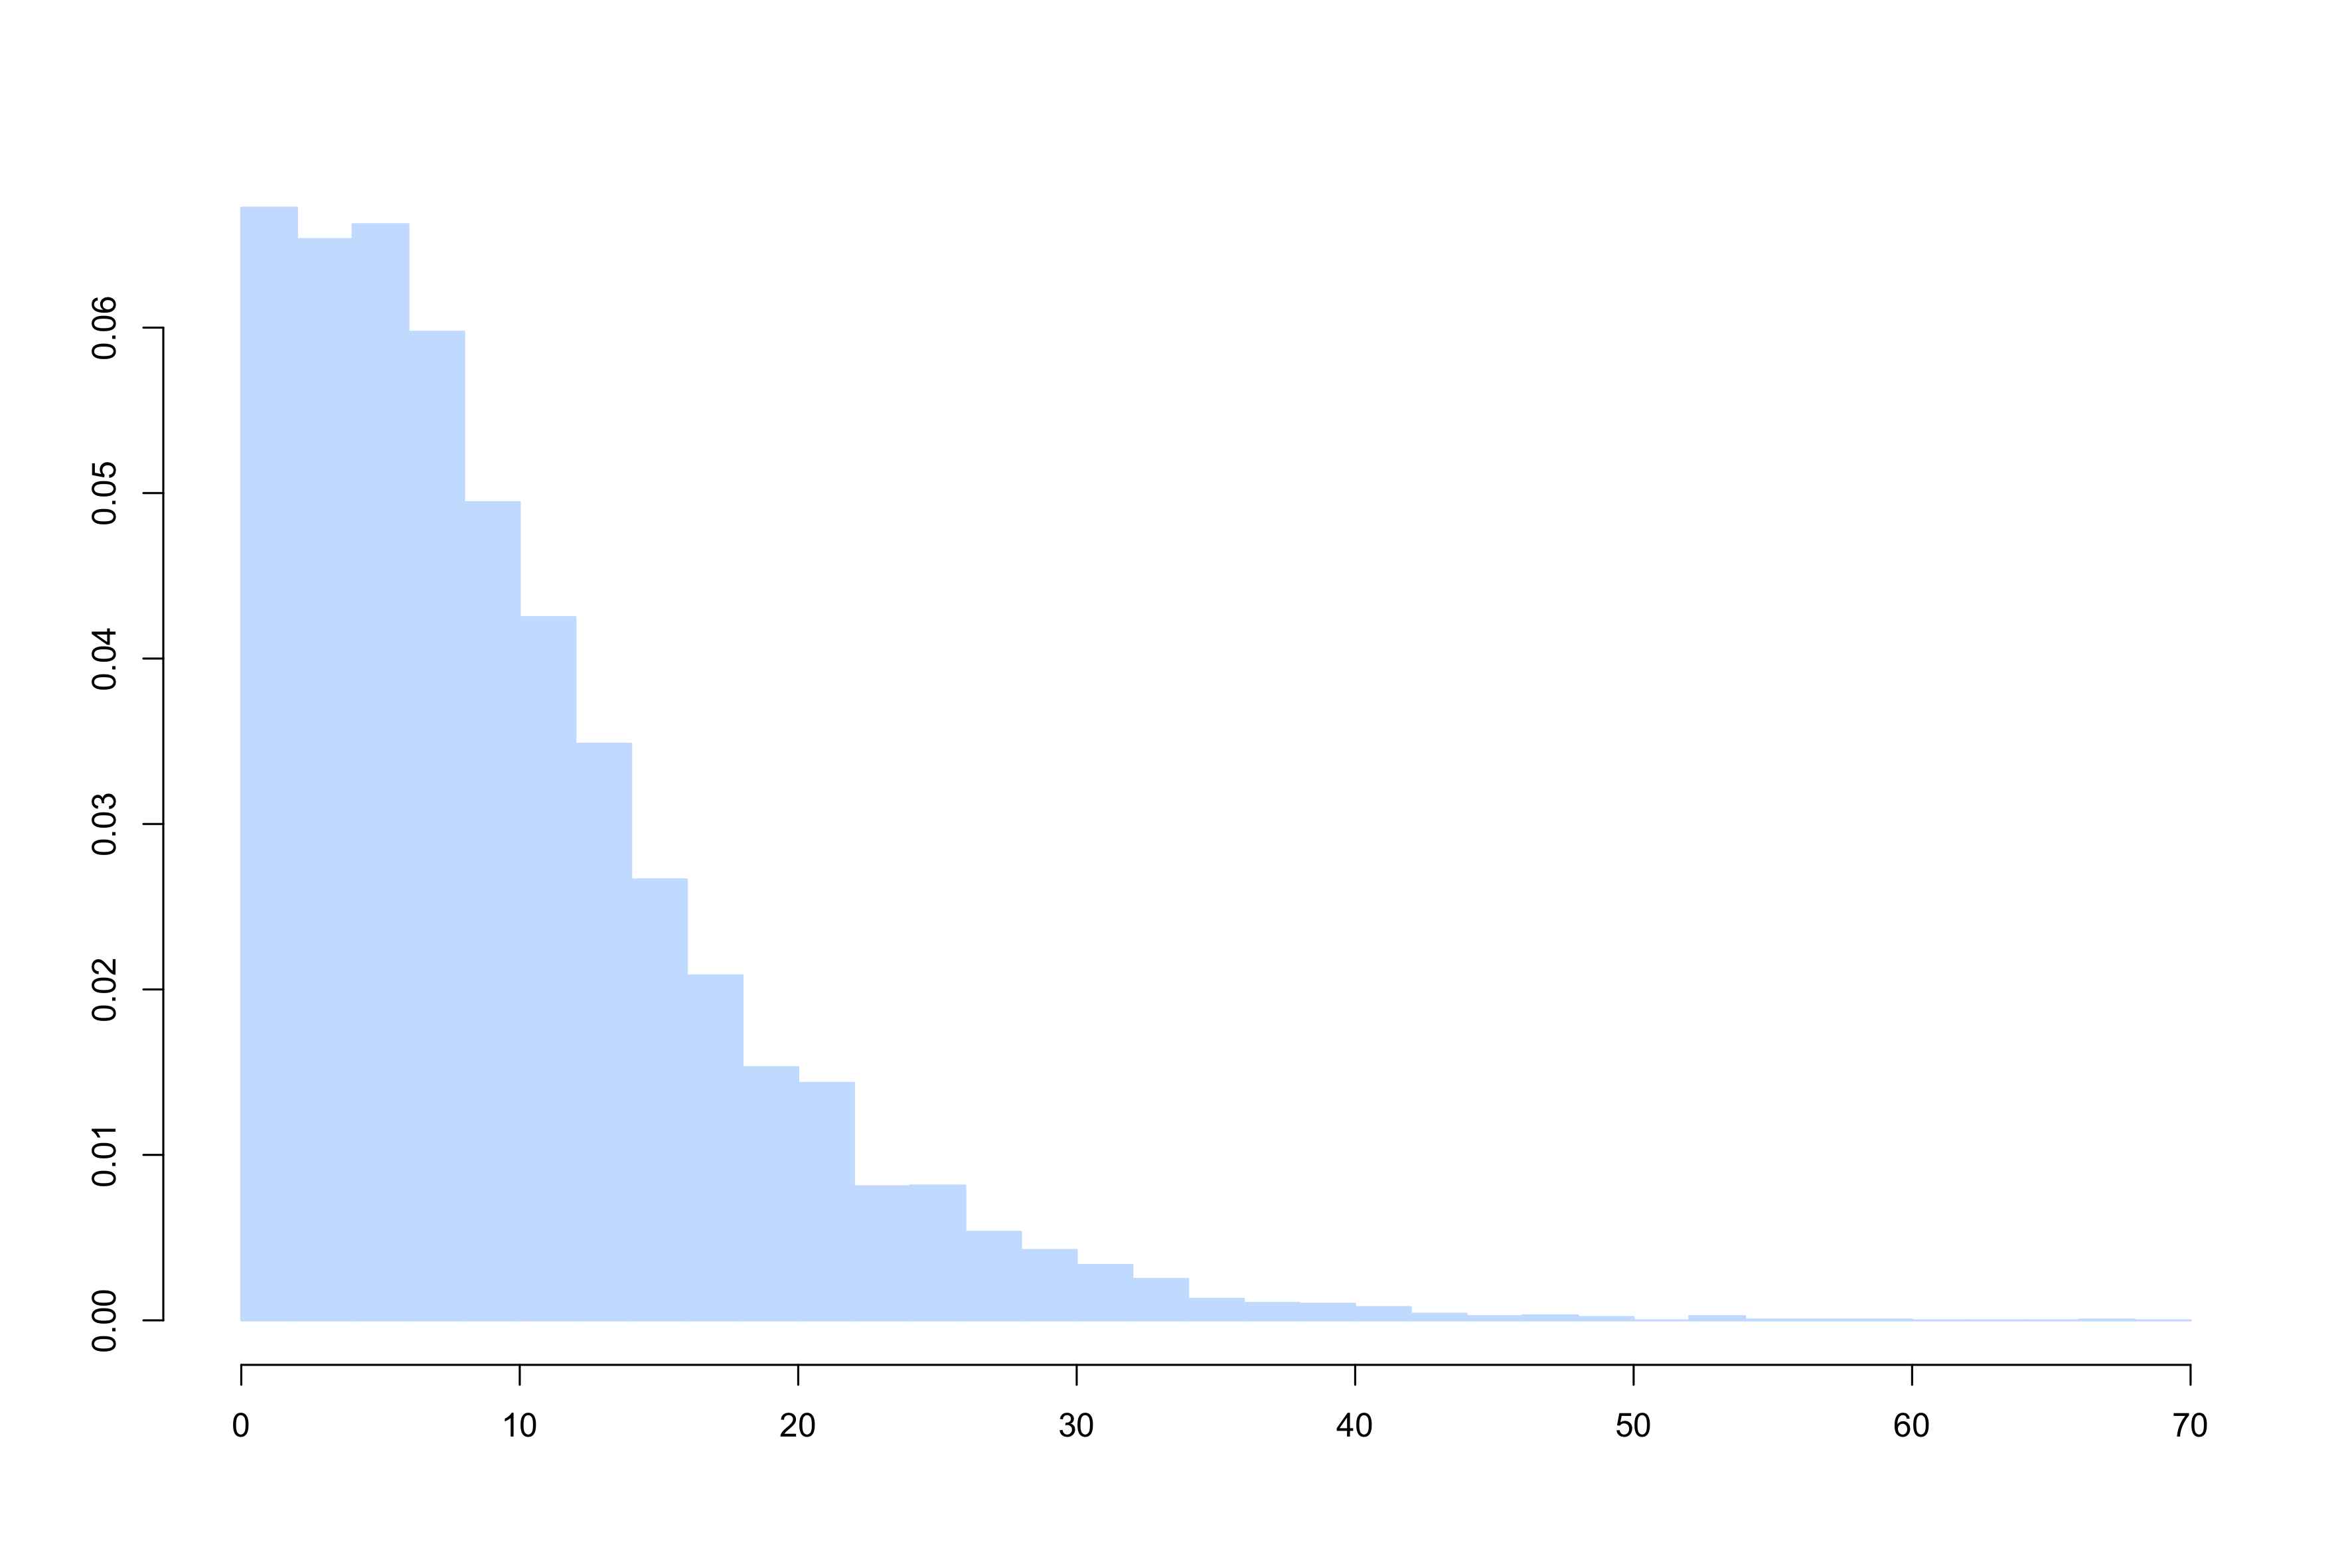
\includegraphics[width=10cm]{poisson_gamma.png}
\caption{Histograma de las simulaciones de $p \sim Pg(2, 1, 5)$.}
\label{fig:poga}
\end{figure}

Es común en inferencia estadística bayesiana que las distribuciones posteriores de las cuales queremos obtener muestras, sean conocidas salvo por una constante. En estos casos, el método de la transformada inversa no se puede utilizar ya que no podemos obtener la inversa generalizada $F^{-1}$. Sin embargo, si la distribución de interés es discreta, existe una manera sencilla de aproximar esta constante. A continuación, se presenta un ejemplo para ilustrar esta técnica utilizada en la sección \ref{elmodelo} para obtener muestras de este tipo.\\

Sea $X$ una variable aleatoria con distribución Poisson, $X \sim Po(\lambda),$ $\lambda > 0$. La función de probabilidad de $X$ está dada por
$$P(X = x) = \frac{\lambda ^ x}{x!}e^{-\lambda}$$ con $S_X = \lbrace 0, 1, 2, \dots \rbrace$. Supongamos ahora que no conocemos la constante $e^{-\lambda}$ y que únicamente sabemos que $$P(X = x) \propto  \frac{\lambda ^ x}{x!}.$$\\

Como $$\sum_{x \in S_X} P(X = x) = 1,$$ se sigue que $$\sum_{x \in S_X} \frac{\lambda ^ x}{x!} = e^{\lambda}$$ y tenemos que la constante $$e^{-\lambda} = 1 /\sum_{x \in S_X} \frac{\lambda ^ x}{x!}.$$\\

Si se desean obtener muestras de $X$, fijamos un límite $\Lambda >> 0$ y utilizamos la aproximación $$ e^{\lambda} \approx \sum_{x = 0}^{\Lambda} \frac{\lambda ^ x}{x!}$$ para el método de la transformada inversa. A continuación, se presenta el código de R para obtener muestras de una variable aleatoria $X \sim Po(10)$ y se compara la función masa de probabilidad empírica con la "verdadera" dada por la función $\mathtt{dpois}$.\\

\begin{figure}[H] 
\centering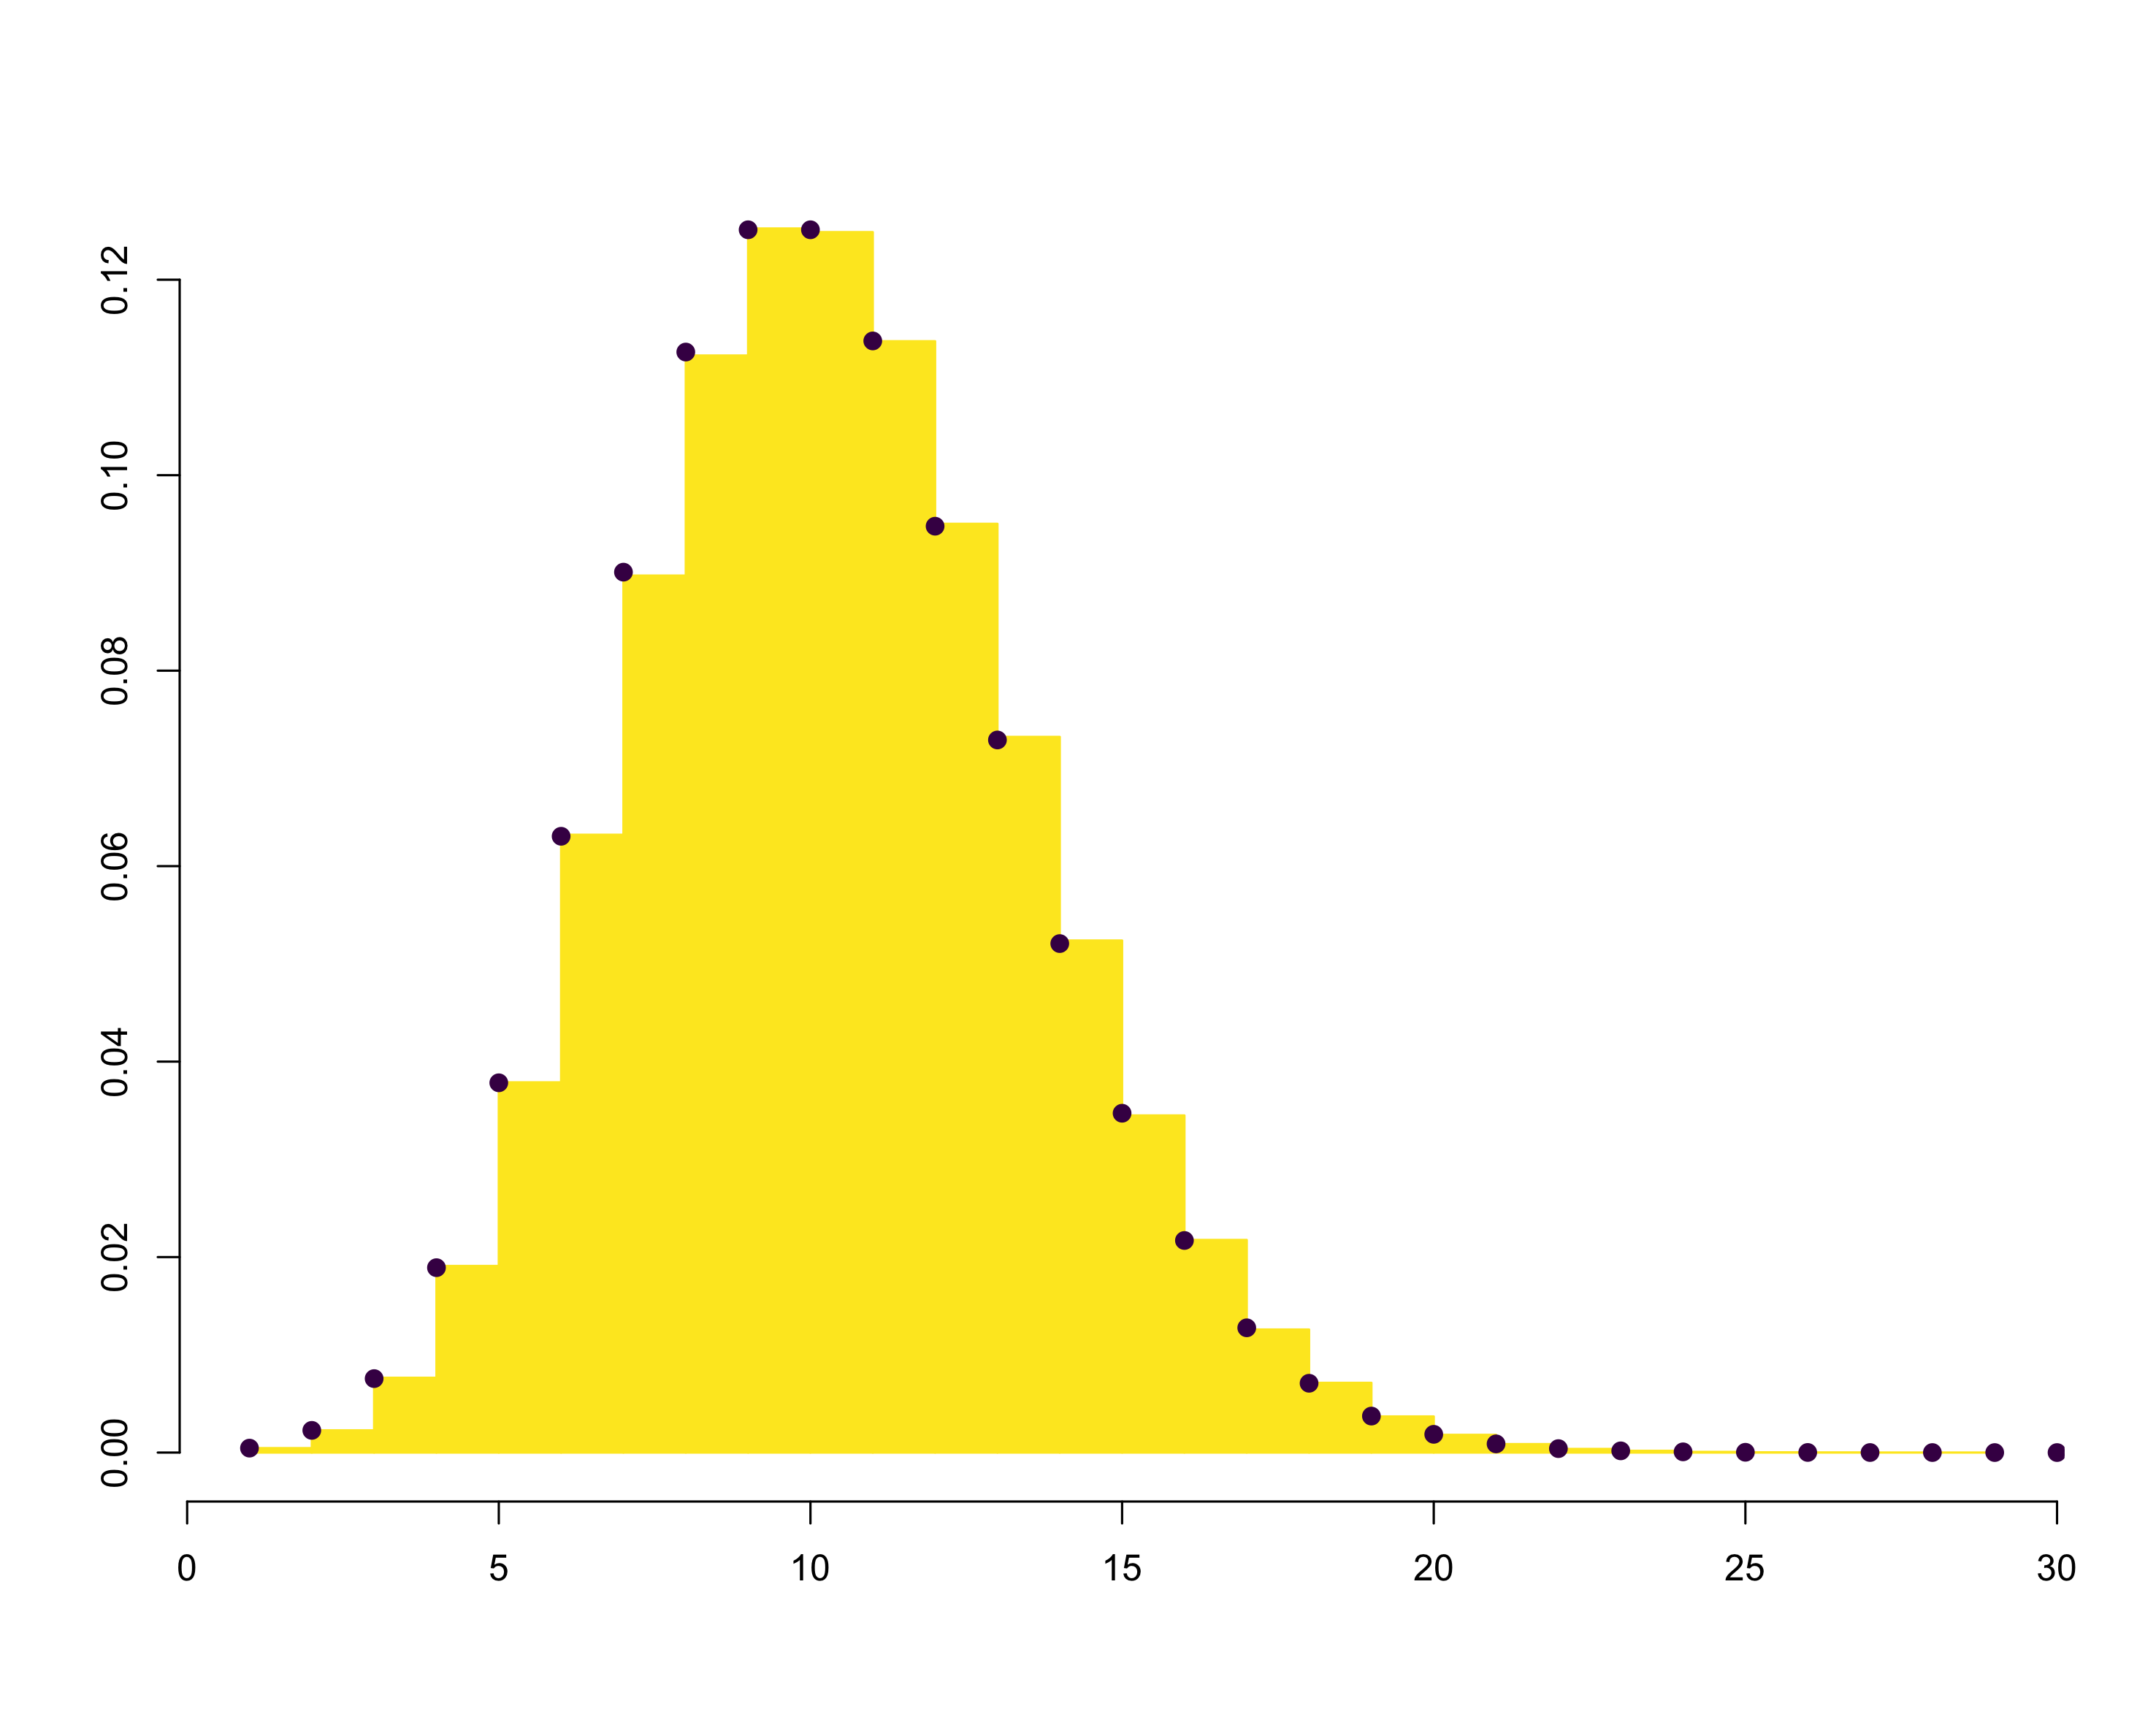
\includegraphics[width=10cm]{poisson.png}
\caption{Histograma de las simulaciones de $f \sim Po(10)$ con la masa de probabilidad real (puntos).}
\label{fig:poisson}
\end{figure}

\begin{lstlisting}
# Poisson

tol <- 10e-30
x <- 0
acum <- 0
lambda <- 10
prob <- 1
f <- c()

while(prob > tol) {
 densidad <- x * log(lambda) - lgamma(x + 1)
 densidad <- exp(densidad)
 acum <- acum + densidad
 prob <- densidad/acum
 f <- c(f, densidad)
 x <- x + 1
}

pois <- f / acum

muestra <- sample(1:x, size = 1e6, replace = TRUE, prob = pois)

hist(muestra, probability = TRUE)
points(1:x, dpois(1:x, lambda = 10))

\end{lstlisting}


\subsection{Métodos de aceptación y rechazo}
\label{aceptacion}

Estos métodos se utilizan cuando no se pueden obtener simulaciones de la densidad de interés por medio del método de la transformada inversa o con otras transformaciones de variables aleatorias.\\

Si queremos simular observaciones de una variable aleatoria $X\sim f$, buscamos una función de densidad $g$ tal que:

\begin{enumerate}
\item $\{x: f(x) > 0\}\subseteq \{x: g(x) > 0\}$.\\
\item $\exists M \in \mathbb{R}$ tal que $f/g \leq M.$
\end{enumerate}

A la densidad $f$ la llamaremos \textit{distribución objetivo} y a $g$ \textit{distribución candidata}. El algoritmo mencionado en \citet{casella} para simular observaciones de $X \sim f$ es:

\begin{enumerate}
\item Generar una observación $y$ de $Y\sim g$.
\item Generar una observación $u$ de $U\sim U(0,1)$ independiente de $Y$.
\item Si $u \leq \frac{1}{M}\frac{f(y)}{g(y)}$, aceptar $y$ como una observación de $X$.\\
\end{enumerate}

En opinión de quien redacta este documento, la razón por la cual este algoritmo funciona no es obvia. A continuación se muestra un resultado que permitirá al lector comprender el funcionamiento del método.\\

\textbf{Método de aceptación y rechazo.} Sean $X\sim f$ y $Y \sim g$ dos variables aleatorias tales que $S_X \subseteq S_Y$ y $\exists M \in \mathbb{R}$ tal que $f(x)/g(x) \leq M$ $\forall x \in S_X$. Sea $x \in S_X$, entonces $$P\left\lbrace Y \leq x \  \vline \ U\leq \frac{1}{M}\frac{f(Y)}{g(Y)}\right\rbrace = P\{X\leq x\}.$$\\

\textit{Demostración.}
$$P\left\lbrace Y \leq x \  \vline \ U\leq \frac{1}{M}\frac{f(Y)}{g(Y)}\right\rbrace = \frac{P\left\lbrace Y\leq x, \ U \leq \frac{f(Y)}{Mg(Y)}\right\rbrace}{P\left\lbrace U \leq \frac{f(Y)}{Mg(Y)}\right\rbrace}.$$ Para el denominador tenemos 
\begin{align*}
P\left\lbrace U \leq \frac{f(Y)}{Mg(Y)}\right\rbrace &= \int_{S_Y}P\left\lbrace U \leq \frac{1}{M}\frac{f(y)}{g(y)} \ \vline \ Y=y\right\rbrace g(y) dy\\
&= \int_{S_Y}\int_0^{M^{-1} f(y)/g(y)} g(y)du \ dy\\
&= \int_{S_Y}g(y)\left(\int_0^{M^{-1} f(y)/g(y)} du\right)\ dy\\
&= \int_{S_Y}\frac{1}{M}f(y) \ dy\\
&= \frac{1}{M}
\end{align*}

y para el numerador tenemos
\begin{align*}
P\left\lbrace Y \leq x, \ U \leq \frac{1}{M}\frac{f(Y)}{g(Y)}\right\rbrace &= \int_{-\infty}^x\int_0^{M^{-1} f(y)/g(y)} du \ g(y) \ dy\\
&= \int_{-\infty}^x \frac{f(y)}{M} \ dy\\
&= \frac{1}{M} F(x).
\end{align*}

Por lo tanto, tenemos que $$P\left\lbrace Y \leq x \  \vline \ U\leq \frac{1}{M}\frac{f(Y)}{g(Y)}\right\rbrace = F(x) = P\{X \leq x\}.$$\\

Al seguir esta demostración, podemos notar que el algoritmo no depende de las constantes de normalización, por lo que se pueden utilizar funciones proporcionales a $f$ y $g$ para las que se conozca la constante $M$.\\

Encontrar una cota $M$ para el cociente $f/g$ implica que se cuenta con una infinidad de cotas para este cociente. El atento lector habrá notado en la demostración anterior que $P\left\lbrace U \leq \frac{1}{M}\frac{f(Y)}{g(Y)}\right\rbrace = 1/M$, es decir, la probabilidad de aceptación en el algoritmo es de $\frac{1}{M}$. Este resultado muestra la importancia de elegir la constante $M$ tan pequeña como sea posible, ya que una baja probabilidad de aceptación puede resultar en un algoritmo costoso e ineficiente en términos computacionales.\\

En teoría, sería útil generar un algoritmo para optimizar la constante $M$ y que tenga el menor valor posible. Sin embargo, en la práctica se debe tomar en cuenta el uso que se va a hacer del algoritmo de aceptación y rechazo. Por ejemplo, si solamente se necesita generar una muestra aleatoria, el costo de optimizar $M$ puede ser mucho mayor a la pérdida de eficiencia por utilizar una $M$ más grande.\\

Ahora se presenta un ejemplo del método de aceptación y rechazo para obtener muestras de una distribución gamma $Ga(2, 1).$ Como distribución candidata utilizamos $g \sim Exp(0.5).$ El histograma de las simulaciones se encuentra en la figura \ref{fig:acep_rech}.\\

\begin{lstlisting}
f <- function(x) {dgamma(x, shape = 2, rate = 1)}
g <- function(x) {dexp(x, rate = 0.5)}
h <- function(x) {f(x)/g(x)}

set.seed(42)

n.sim <- 1e5

M <- 4/exp(1)

proposal <- rexp(n = n.sim, rate = 0.5)

u <- runif(n = n.sim)

aceptados <- u <= 1/M * h(proposal)

sample.f <- proposal[aceptados]
\end{lstlisting}

\begin{figure}
\centering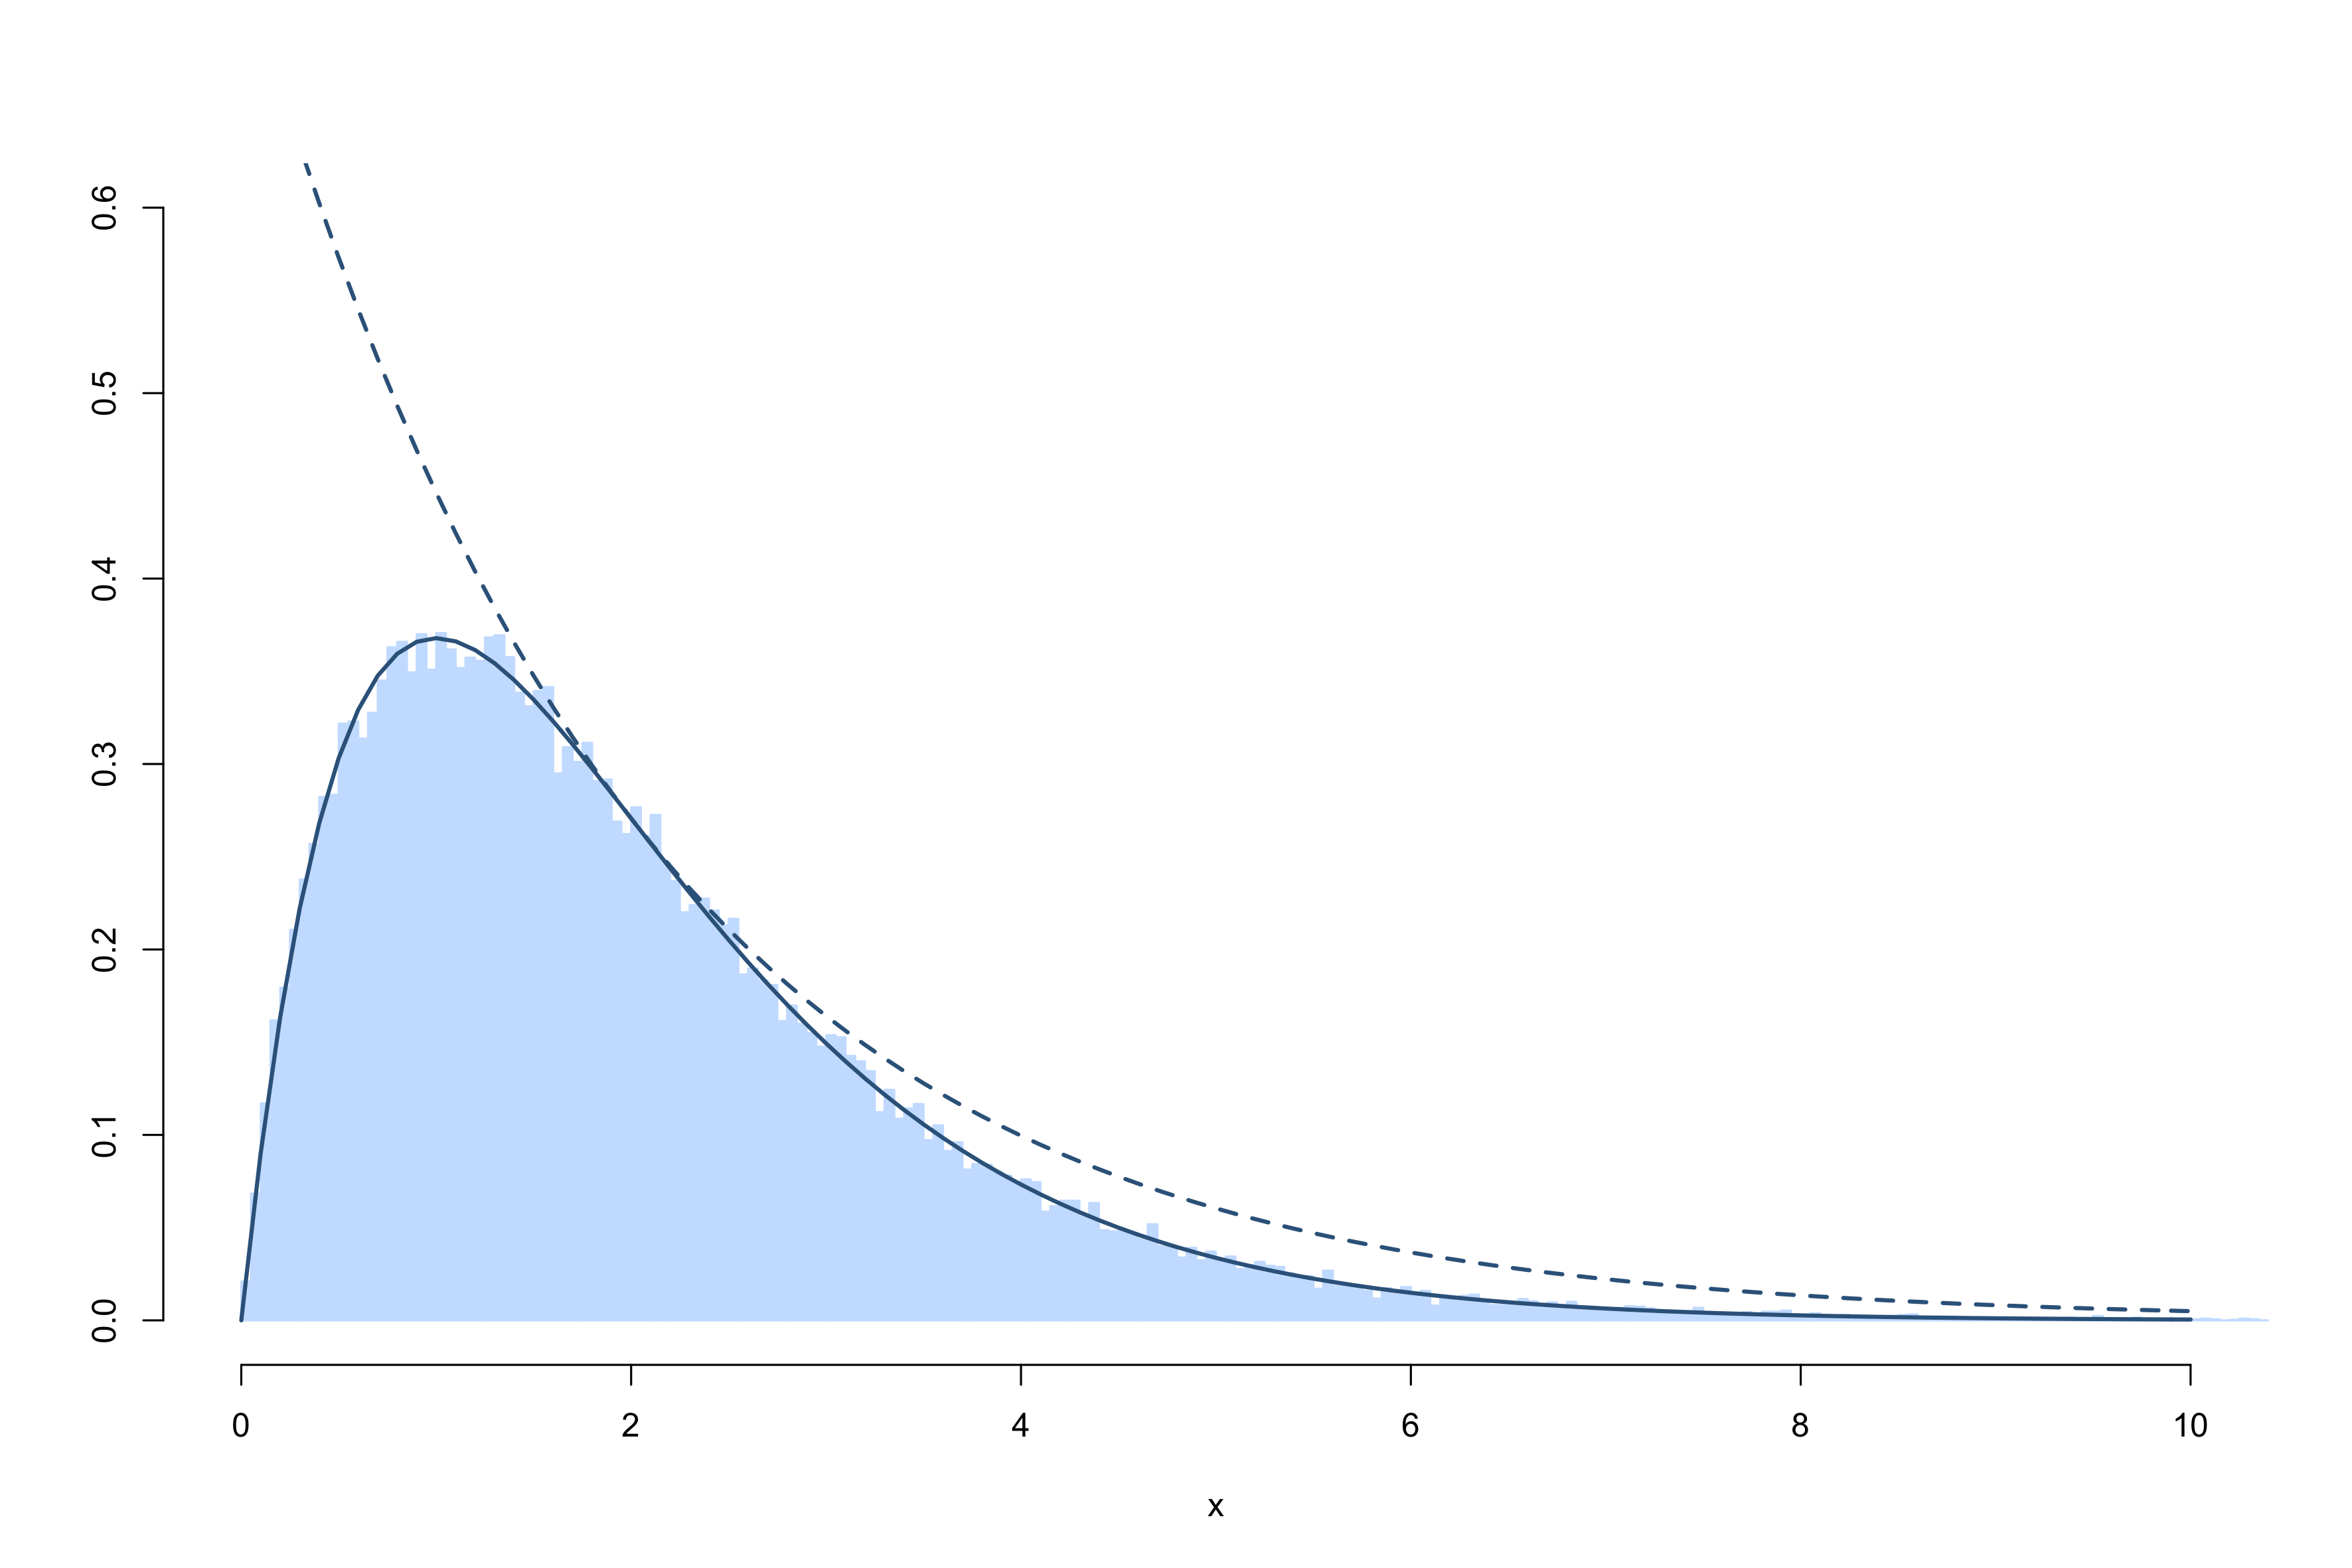
\includegraphics[width=10cm]{aceptacion_rechazo.png}
\caption{Histograma de las simulaciones de $Ga(2, 1)$, con la densidad real $g(x)$ (línea continua) y la curva $M f(x)$ (línea punteada).}
\label{fig:acep_rech}
\end{figure}

Es importante resaltar que es preferible utilizar el método de la transformación inversa cuando sea posible, ya que cada observación generada por medio de ese método es utilizada como observación de $F$. Por el contrario, en los métodos de aceptación y rechazo se generan observaciones ``basura" (rechazadas) que no son utilizadas, por lo que se necesitan más iteraciones para obtener una muestra de tamaño $n$.\\

En R, es recomendable utilizar cuando sea posible alguna de las funciones ya implementadas para simular variables aleatorias como $\mathtt{rnorm}$, $\mathtt{runif}$, $\mathtt{rgamma}$, etc., ya que están optimizadas para minimizar el tiempo de las simulaciones y se puede consultar su documentación con el comando $\mathtt{help()}$ o $\mathtt{?}$.\\

Los algoritmos presentados en esta sección son la base de la simulación de variables aleatorias. Con ellos, se pueden generar muestras de una gran cantidad de distribuciones. Además, es importante resaltar que si tenemos los medios para generar observaciones de $X \sim F$, entonces se pueden generar directamente observaciones de cualquier transformación de esta variable aleatoria que tenga la forma $Y = g(X)$, simplemente evaluando la función $g$ en cada observación simulada de $X$.

Para finalizar este capítulo, exploraremos de manera superficial el tema de cópulas. Qué son, para qué se utilizan y cómo se construyen.\\

\subsection{Cópulas} \label{sec_copulas}

Las cópulas son funciones que se utilizan para construir distribuciones conjuntas a través de sus distribuciones univariadas. También se pueden entender las cópulas como funciones de distribución multivariadas con marginales $U(0, 1)$ \citep{nelsen}. Formalmente, se tiene la siguiente definición.\\

\textbf{Definición.} Una cópula $\C$ es una función 
\begin{align*}
\C: [0,1]\times[0,1]&\to [0,1]\\
(u,v) &\to \C(u,v)
\end{align*} tal que:
\begin{enumerate}
\item $\forall \ u,v \in [0,1]$
\begin{itemize}
\item $\C (u,0) = \C (0,v) = 0$
\item $\C(u,1) = u$
\item $\C(1, v) = v$
\end{itemize}
\item $\forall \ u_1, u_2, v_1, v_2 \in [0,1]$ tales que $u_1 \leq u_2$ y $v_1 \leq v_2$  $$\C (u_1,v_1)+\C (u_2,v_2) - \C(u_1,v_2) - \C(u_2,v_2)\geq 0.$$\\
\end{enumerate}

El principal interés en las cópulas es poder modelar la estructura de dependencia entre las componentes de vectores aleatorios. Pero antes de meternos en estos temas, es importante entender cómo se utilizan las cópulas para construir distribuciones conjuntas.\\ 

El siguiente teorema es el resultado más importante de la teoría de cópulas \citep{copula_modeling}. Su importancia recae en que demuestra la relación que existe entre las cópulas y las funciones de distribución. El enunciado es como sigue.\\

\begin{theorem}[Teorema de Sklar]
\label{sklar}
Sea $F$ una función de distribución conjunta con marginales $F_X$ y $F_Y$. Entonces, existe una cópula $\C$ tal que $\forall \ x,y \in \R$ $$F(x,y) = \C(F_X(x), F_Y(y)).$$ Si $F_X$ y $F_Y$ son continuas, entonces $\C$ es única.\\

De la misma manera, si $\C$ es una cópula y $F_X$, $F_Y$ son funciones de distribución univariadas, entonces la función $F$ definida como $$F(x, y) = \C(F_X(x), F_Y(y))$$ es una función de distribución conjunta con marginales $F_X$ y $F_Y$.\\
\end{theorem}

La demostración de este teorema se puede encontrar en \citet{nelsen}. A la cópula $\C$ del teorema \ref{sklar} se le llama \textit{cópula de $X$ y $Y$} y se denota $\C_{XY}$.\\

Resaltemos dos importantes conclusiones que podemos sacar del teorema de Sklar. Primero, si tenemos observaciones de un vector bivariado $(X, Y)$ con distribuciones marginales continuas, \eqref{sklar} nos dice que la cópula correspondiente a su distribución conjunta es única. Por lo tanto, es útil estimarla a partir de los datos para poder modelar la estructura de dependencia entre $X$ y $Y$.\\

Por otro lado, el teorema de Sklar es una herramienta para crear distribuciones conjuntas con la estructura de dependencia que más convenga a nuestra aplicación. En específico, si tenemos dos distribuciones marginales $F_X$ y $F_Y$, junto con una estructura de dependencia modelada a través de una cópula $\C$, entonces podemos crear una función de distribución conjunta que refleje esta estructura utilizando $F(x, y) = \C (F_X(x), F_Y(y))$.\\

Un caso singular de esta estructura de dependencia es cuando las componentes de un vector aleatorio son independientes. La forma más común de estudiar relaciones entre las componentes es con el coeficiente de correlación de Pearson, el cual solamente cuantifica la dependencia lineal entre variables. Esto significa que si las componentes son independientes, entonces el coeficiente de correlación vale cero. Sin embargo, un coeficiente de correlación cero no implica independencia entre las componentes (ver figura \ref{fig:panel_corr}).\\

En contraste con el coeficiente de correlación, la teoría de cópulas tiene una forma única de modelar independencia entre las componentes de un vector aleatorio. El teorema \ref{independencia} muestra cómo se modela esta independencia con una cópula específica.\\

\begin{theorem}
\label{independencia}
Sean $X$ y $Y$ dos variables aleatorias continuas con función de distribución conjunta $F$ y marginales $F_X$ y $F_Y$ respectivamente. Entonces $X$ y $Y$ son independientes si y solo si $\C_{XY} = \Pi$, donde $\Pi$ es la cópula producto dada por $\Pi (u,v) = uv.$
\end{theorem}

\begin{proof}\mbox{}\\*
$\implies\big)$ Si $X$ y $Y$ son independientes, entonces
\begin{equation} \label{conjunta}
F(x, y) = F_X(x)F_Y(y).
\end{equation}

Por el teorema \ref{sklar}, como $F_X$ y $F_Y$ son continuas, sabemos que existe una única cópula $\C_{XY}$ tal que
\begin{equation} \label{copula}
F(x, y) = \C_{XY}(F_X(x), F_Y(y)).
\end{equation}

Juntando \eqref{conjunta} y \eqref{copula} tenemos que $\C_{XY}(F_X(x), F_Y(y)) = F_X(x)F_Y(y)$, por lo que $\C_{XY} = \Pi$.\\

$\impliedby \big)$ Por el teorema \ref{sklar} existe una única $\C_{XY}$ tal que $F(x, y) = \C_{XY}(F_X(x), F_Y(y))$. Si $\C_{XY} = \Pi$ tenemos que $F(x, y) = F_X(x)F_Y(y)$, es decir, $X$ y $Y$ son independientes.\\
\end{proof}

Como en análisis de supervivencia es común trabajar con la función de supervivencia conjunta en vez de la distribución, introducimos el concepto de las cópulas de supervivencia. Buscamos ahora una función $\widehat{C}$ tal que
\begin{equation} \label{suvcop}
S(x, y) = \widehat{C}(S_X(x), S_Y(y)),
\end{equation}
donde $S$ es la función de supervivencia conjunta definida como $$S(x, y ) = P\lbrace X>x, Y>y\rbrace$$ y $S_X$ y $S_Y$ son las funciones de supervivencia marginales.\\

El siguiente resultado nos muestra como construir la función $\widehat{C}$. La demostración se puede encontrar en \citet{nelsen}.\\

\begin{proposition}[Cópulas de supervivencia]
\label{def_cop_surv}
Sean X y Y dos variables aleatorias con distribuciones marginales $F_X$ $F_Y$ y cópula $C$. Entonces, la función $\widehat{C}$ definida como $$\widehat{C}(u, v) = u + v - 1 + C(1-u, 1-v)$$ cumple la ecuación \eqref{suvcop}.\\
\end{proposition}

Antes de introducir medidas de concordancia alternativas a la correlación de Pearson, veamos un ejemplo de por qué necesitamos medidas alternativas para ver relaciones no lineales. Este ejemplo es tomado de \citet{copula_modeling} y consiste en simular un vector aleatorio $X = (X_1, X_2)$ donde $X_1 \sim \mathcal{N}(0, 1)$ y $$X_2 = \begin{cases}
X_1 & p = 0.5\\
-X_1 & p = 0.5
\end{cases}.$$\\

El diagrama de dispersión se muestra en la figura \ref{fig:panel_corr}. Siguiendo el ejemplo de \citet{copula_modeling}, se presenta también un diagrama de dispersión para un vector bivariado con componentes normales estándar generadas de manera independiente. El código para generar las simulaciones es el siguiente.\\

\begin{lstlisting}
n.sim <- 1e4

set.seed(42)
x1 <- rnorm(n.sim)
u <- runif(n.sim)
x2 <- ifelse(u <= 0.5, x1, -x1)
y <- rnorm(n.sim)

cor(x1, x2)
cor(x1, y)
\end{lstlisting}

\begin{figure}
    \centering
    \begin{subfigure}[t]{0.45\textwidth}
        \centering
        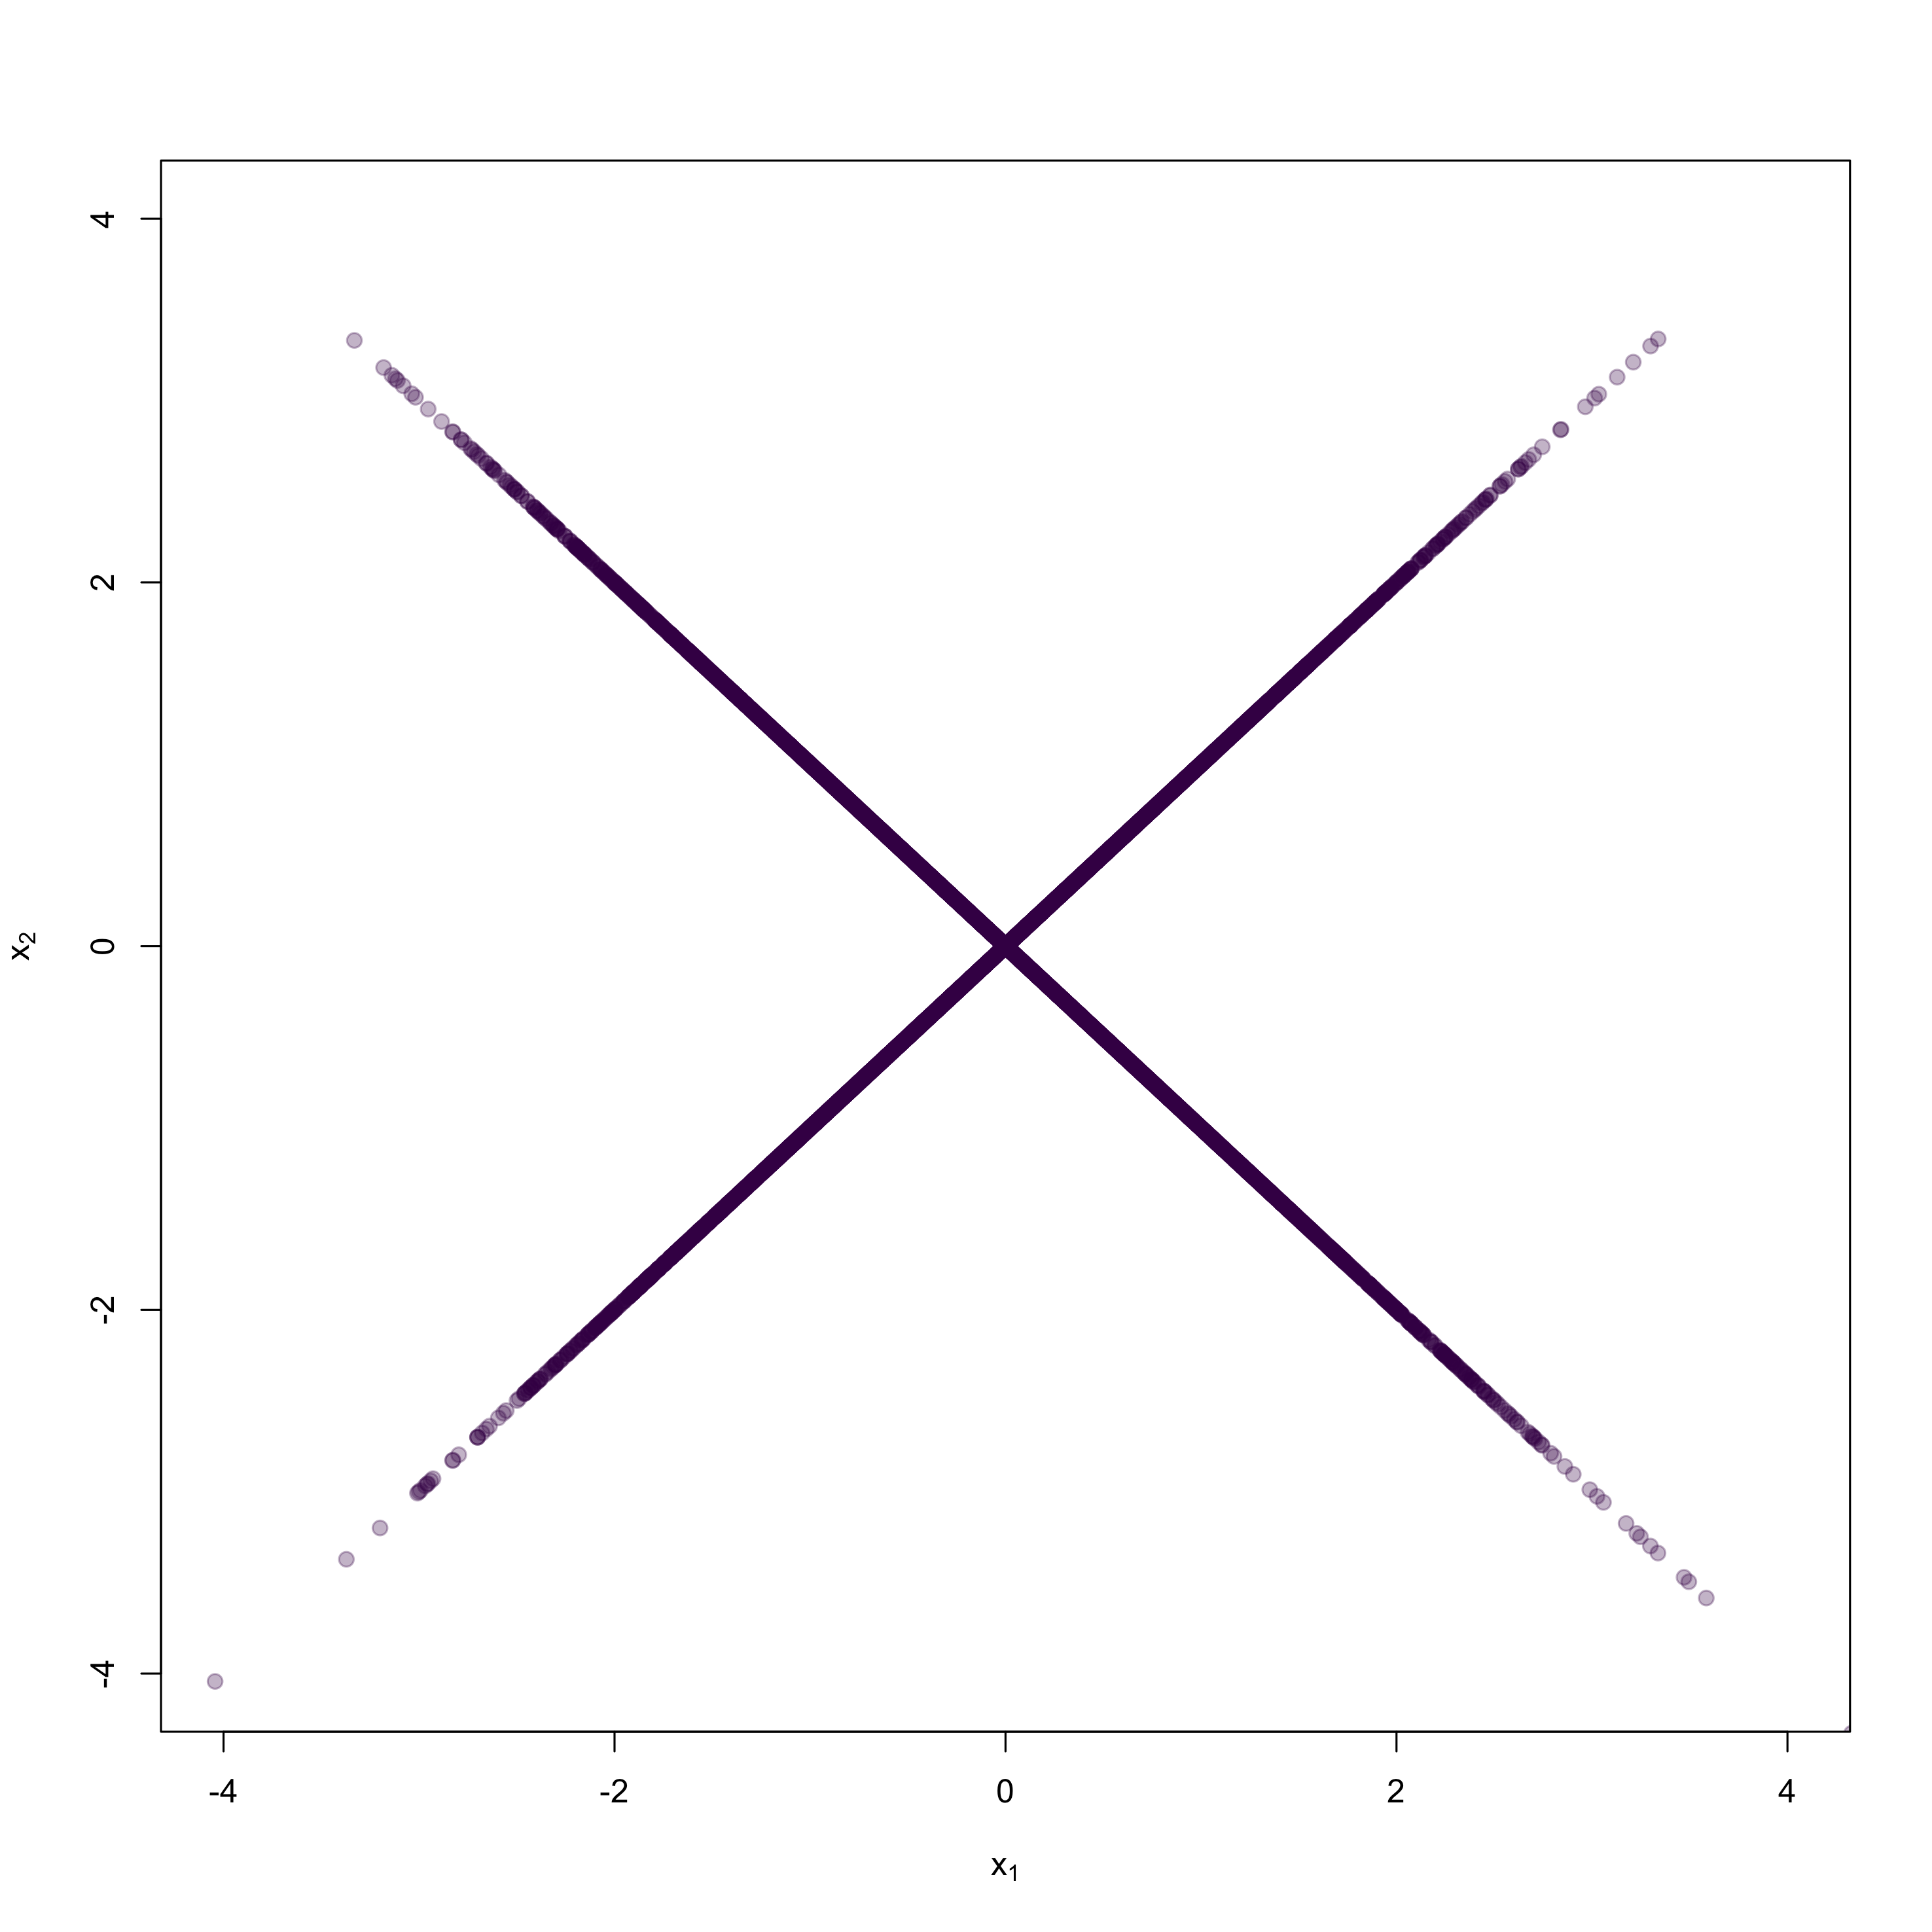
\includegraphics[width=\linewidth]{correlation.png} 
        \caption{Diagrama de dispersión para valores simulados de $(X_1, X_2)$.} \label{fig:corr1}
    \end{subfigure}
    \hfill
    \begin{subfigure}[t]{0.45\textwidth}
        \centering
        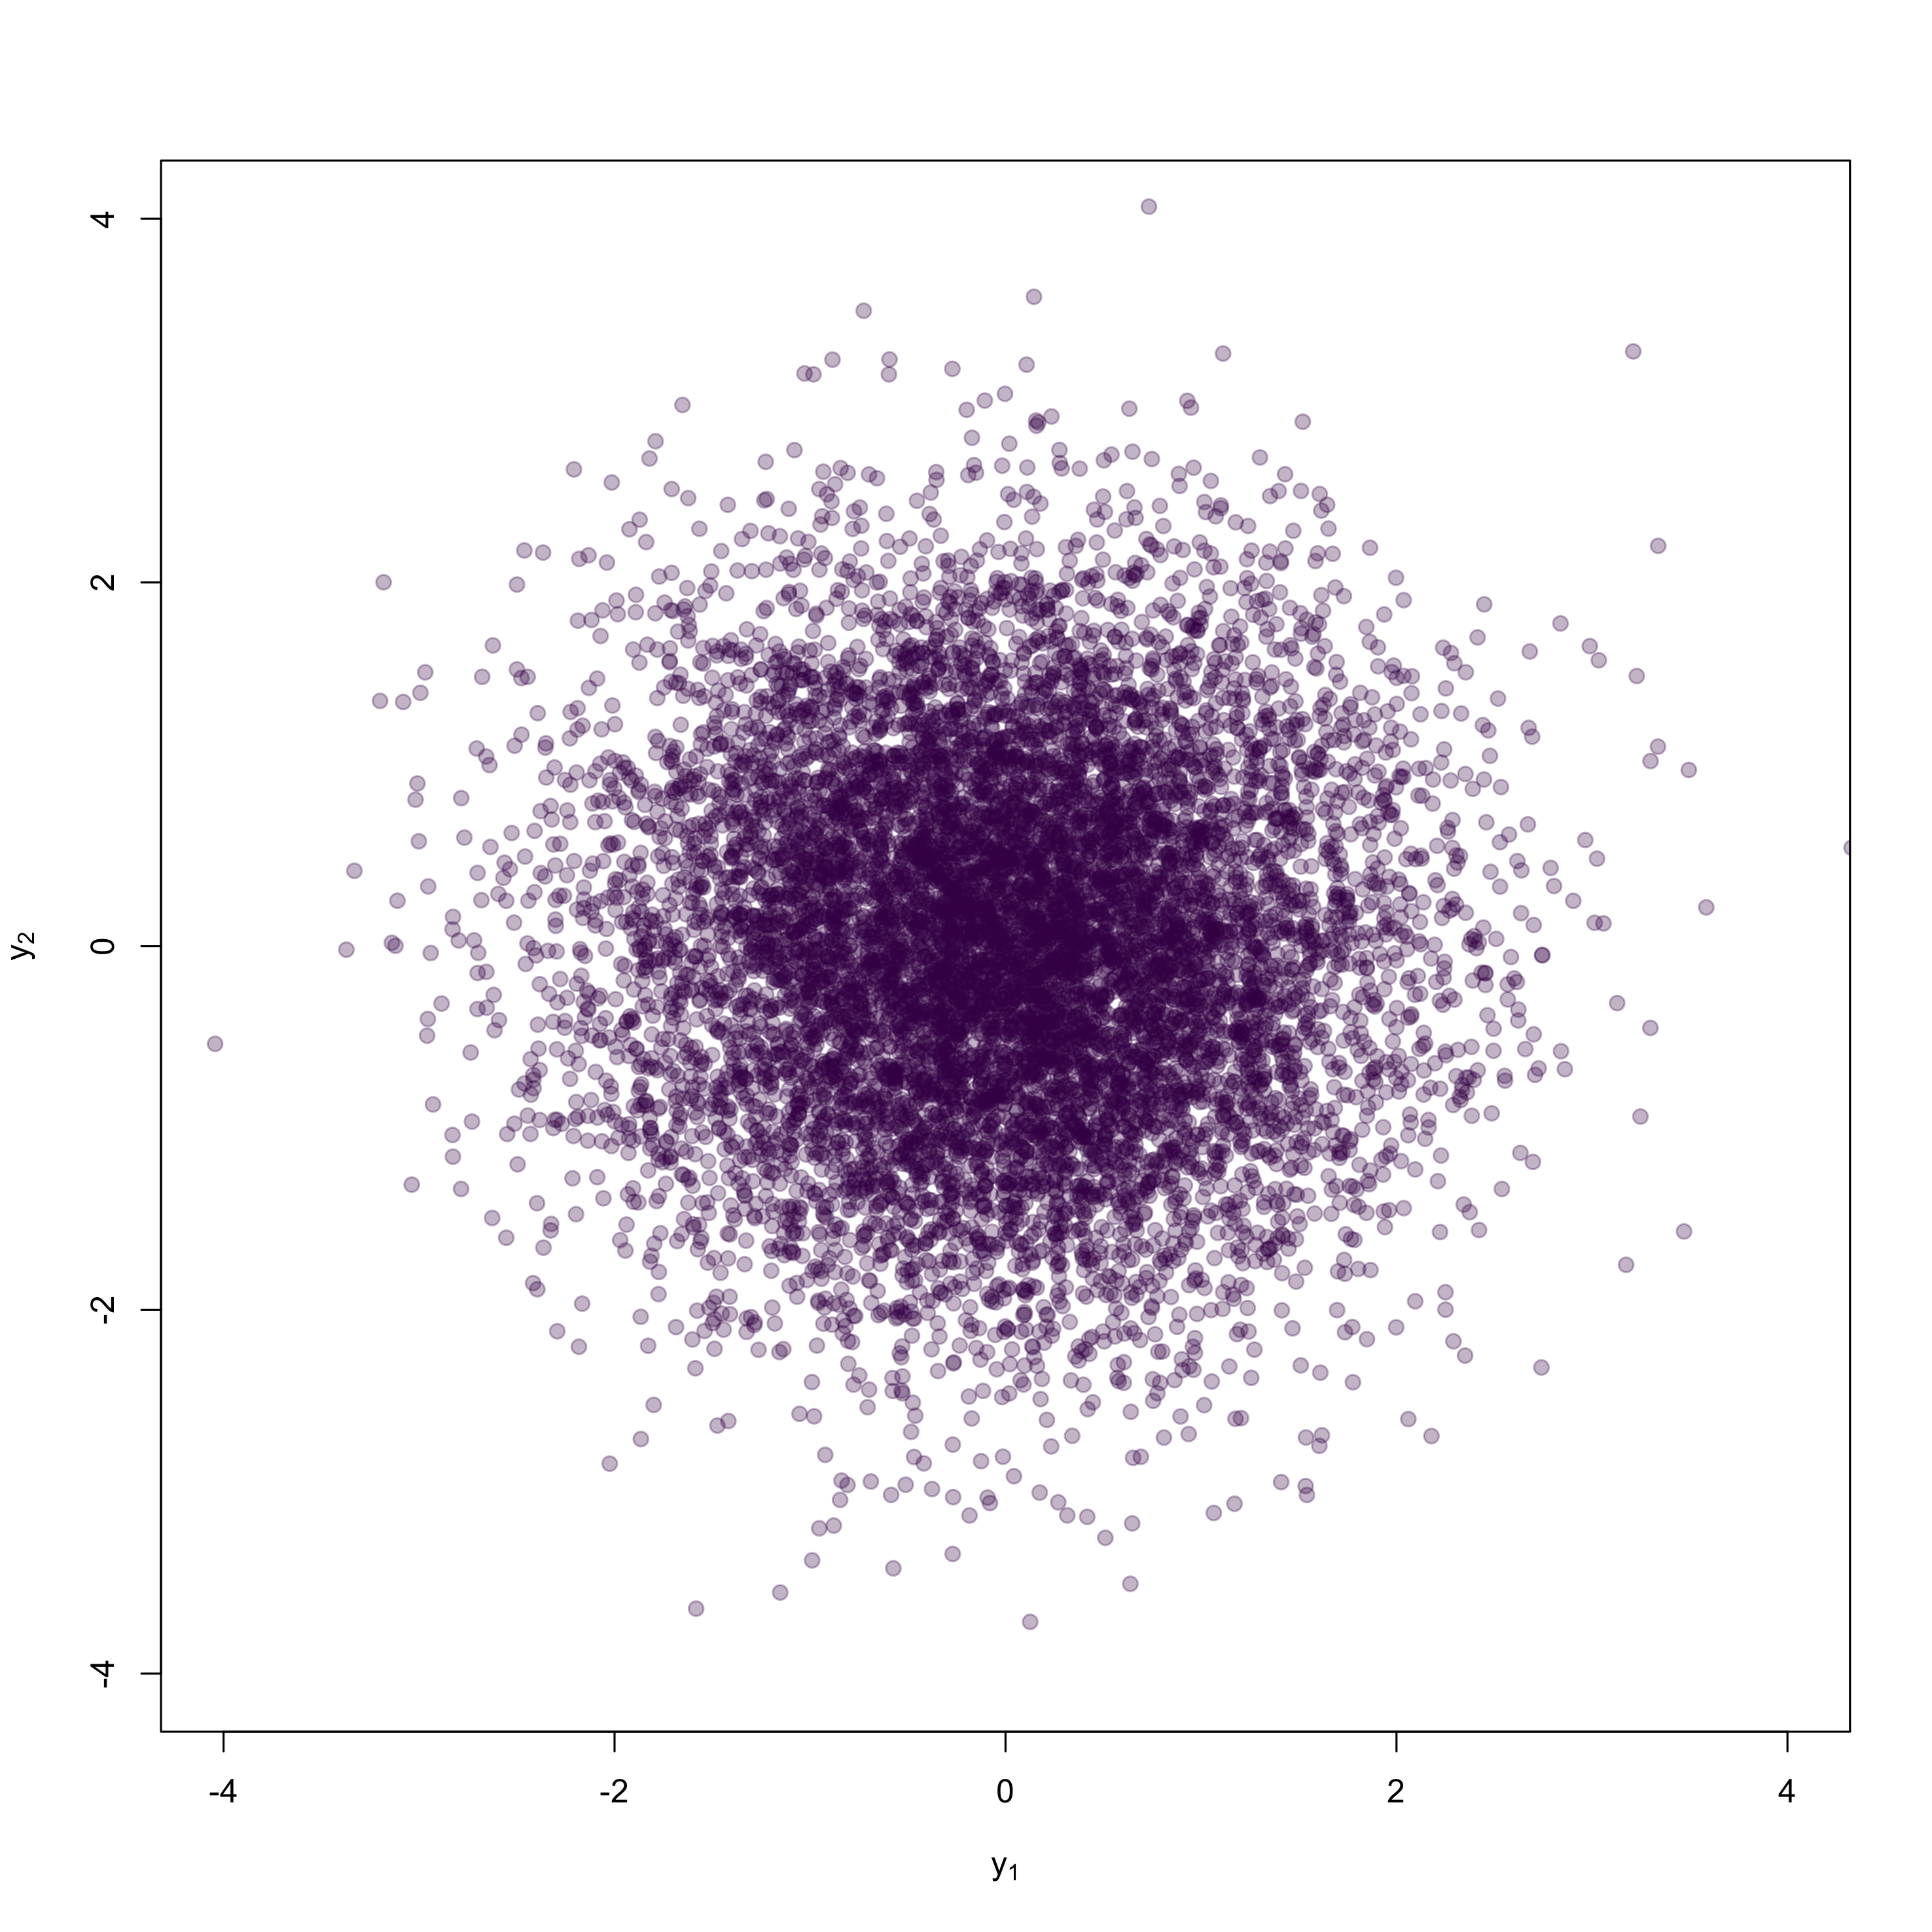
\includegraphics[width=\linewidth]{correlation_ind.png} 
        \caption{Diagrama de dispersión para valores simulados de $(Y_1, Y_2)$ independientes.} \label{fig:corr2}
    \end{subfigure}
    
    \caption{Simulaciones de vectores aleatorios con marginales $\mathcal{N}(0, 1)$. $\mathtt{cor(x1, x2)} = -0.02$ y $\mathtt{cor(y1, y2)} = -0.01$.}
    \label{fig:panel_corr}
\end{figure}

Viendo la figura \ref{fig:panel_corr}, es claro que las componentes del vector $X$ tienen una estructura de dependencia completamente distinta a las componentes del vector $Y$. Sin embargo, ambos valores estimados del coeficiente de correlación de Pearson son parecidos y muy cercanos a cero. Se tomó este ejemplo porque ilustra de gran manera que el coeficiente de correlación no determina la estructura de dependencia y resalta lo importante que es visualizar los datos con los que vamos a trabajar antes de lanzarnos a hacer cualquier otra cosa.\\

Ahora hablemos de medidas de concordancia alternativas a la correlación. Solamente hablaremos de las dos más comunes que son la Tau de Kendall y la Rho de Spearman.\\


\subsubsection{Tau de Kendall}
\textbf{Definición.} Sean $(X_1, Y_1)$ y $(X_2, Y_2)$ dos vectores aleatorios independientes e idénticamente distribuidos, con función de distribución $F$. Se define la tau de Kendall, denotada $\uptau_{XY}$, como $$\uptau_{XY} = P\{(X_1-X_2)(Y_1-Y_2)>0\} - P\{(X_1-X_2)(Y_1-Y_2)<0\}.$$

Un valor más grande de $\uptau_{XY}$ significa que es más probable que un par de observaciones del vector aleatorio $(X, Y)$ sea concordante, es decir, que valores `grandes' de $X$ vienen acompañados de valores `grandes' de $Y$ o valores `chicos' de $X$ vienen acompañados de valores `chicos' de $Y$.\\

Estudiemos ahora algunas propiedades de la tau de Kendall.

\begin{proposition}
Sean $X$ y $Y$ dos variables aleatorias continuas con cópula $\C$. Entonces
$$\uptau_{XY} = 4\int_{0}^1\int_{0}^1\C(u, v) \ d\C(u, v) - 1.$$ 
\end{proposition}

\begin{proof} Esta prueba es una adaptación de la demostración en \citet{nelsen}.
Por definición, $$\uptau_{XY} = P\{(X_1-X_2)(Y_1-Y_2) > 0\} - P\{(X_1-X_2)(Y_1-Y_2) < 0\}.$$

Como $P\{(X_1-X_2)(Y_1-Y_2) < 0\} = 1-P\{(X_1-X_2)(Y_1-Y_2) > 0\}$, entonces
\begin{equation} \label{tau}
\uptau_{XY} = 2P\{(X_1-X_2)(Y_1-Y_2) > 0\} - 1.
\end{equation}

Como la distribución conjunta de $X$ y $Y$ es $\C(F_X(x), F_Y(y))$, podemos evaluar esta probabilidad en términos de $\C$.

\begin{equation} \label{dobleprob}
P\{(X_1-X_2)(Y_1-Y_2) > 0\} = P\{X_1<X_2, Y_1<Y_2\} + P\{X_2<X_1, Y_2<Y_1\}.
\end{equation}

\begin{align*}
P\{X_1 < X_2, Y_1 < Y_2\} &=\\
\int_{S_X} \int_{S_Y} &P\{X_1 < X_2, Y_1 < Y_2 | X_2 = x, Y_2 = y\} \ d\C(F_X(x), F_Y(y))\\
&= \int_{S_X} \int_{S_Y} P\{X_1 < x, Y_1 < y\} \ d\C(F_X(x), F_Y(y))\\
&= \int_{S_X} \int_{S_Y} \C(F_X(x), F_Y(y)) \ d\C(F_X(x), F_Y(y))\\
&= \int_0^1 \int_0^1 \C(u, v) \ d\C(u, v)
\end{align*}
donde la última igualdad se obtiene con las transformaciones $u = F_X(x)$ y $v = F_Y(y)$.\\

De la misma manera, condicionando sobre $X_1, Y_1$ obtenemos que $$P\{X_2 < X_1, Y_2 < Y_1\} = \int_0^1 \int_0^1 \C(u, v) \ d\C(u, v).$$

Sustituyendo estas expresiones en \eqref{dobleprob} y \eqref{tau} concluimos la prueba.\\
\end{proof}

Aquél que desee saber un poco más sobre el diferencial $d\C(u, v)$, diríjase al apéndice \ref{densidad_copula}.\\

Con el resultado anterior, el curioso lector podrá demostrar las siguientes propiedades de $\uptau_{XY}$:

\begin{enumerate}
\item Si $X$ y $Y$ son independientes, $\uptau_{XY} = 0$.
\item $Y = \alpha X$, $\alpha > 0 \implies \uptau_{XY} = 1$.
\item $Y = \beta X$, $\beta < 0 \implies \uptau_{XY} = -1$.
\end{enumerate}

\subsubsection{Rho de Spearman}

\textbf{Definición.} Sean $X$ y $Y$ dos variables aleatorias con marginales $F_X$ y $F_Y$. Tomando las transformaciones $U = F_X(X)$ y $V = F_Y(Y)$, se define la \textit{rho de Spearman}, denotada $\rho_{XY}$, como
\begin{equation} \label{rho}
\rho_{XY} = \frac{cov(U, V)}{\sqrt{var(U)}\sqrt{var(V)}}.
\end{equation}\\

La definición \eqref{rho} es el coeficiente de correlación de Pearson entre $F_X(X)$ y $F_Y(Y)$. Si además $X$ y $Y$ tienen cópula $\C$, entonces las siguientes definiciones son equivalentes a \eqref{rho}:

\begin{align}
\rho_{XY} &= 12\int_0^1 \int_0^1 C(u, v) \ dudv-3\\
\rho_{XY} &= 12\int_0^1 \int_0^1 uv \ d\C(u,v)-3\\
\rho_{XY} &= 12\int_0^1\int_0^1 \left[ \C(u, v) - uv \right] dudv \label{volumen}.
\end{align}

En \citet{nelsen} se menciona una interesante interpretación de \eqref{volumen}. Se puede ver a $\rho_{XY}$ como una `distancia promedio' entre la distribución de $X$ y $Y$, representada por la cópula $\C$, y la independencia representada por la cópula $\Pi$.\\

Al igual que $\uptau_{XY}$, $\rho_{XY}$ cumple las siguientes propiedades:

\begin{enumerate}
\item Si $X$ y $Y$ son independientes, $\rho_{XY} = 0$.
\item $Y = \alpha X$, $\alpha > 0 \implies \rho_{XY} = 1$.
\item $Y = \beta X$, $\beta < 0 \implies \rho_{XY} = -1$.
\end{enumerate}

Si el lector quiere consultar más sobre \textit{métricas de concordancia} con estas propiedades, diríjase a \citet{nelsen}.\\

En este trabajo solamente haremos referencia a las dos medidas de concordancia ya mencionadas. La característica principal que nos lleva a utilizarlas es que ambas se pueden representar por medio de cópulas, sin utilizar la función de distribución conjunta y sin especificar las funciones de distribución marginales.\\

\newpage

\section{Cadenas de Markov Monte Carlo}	
\label{sec_cadenas}
\epigraph{\itshape The combination of Bayes and MCMC has been called ``arguably the most powerful mechanism ever created for processing data and knowledge".}{---Sharon B. McGrayne, \textit{The Theory That Would Not Die.}}
\subsection{Integración Monte Carlo}

Se conoce como integrácion Monte Carlo a un conjunto de técnicas utilizadas para aproximar integrales. La principal característica de estas técnicas es que se basan en los algoritmos presentados en la sección \ref{simulacion} para realizar las aproximaciones a través de muestras aleatorias. Su funcionamiento es consecuencia de uno de los resultados más famosos de la teoría de probabilidad, la \textit{ley fuerte de los grandes números} que se presenta a continuación.\\

\begin{theorem}[Ley fuerte de los grandes números]
\label{grandes_numeros}
Sea $\lbrace X_i \rbrace$ una sucesión de variables aleatorias independientes e idénticamente distribuidas con valor esperado $E[X_i]=\mu < \infty$. Entonces,
$$P\left\lbrace \lim_{n \to \infty} \frac{\sum_{i=1}^{n} X_i}{n} = \mu \right\rbrace = 1.$$\\
\end{theorem}

Este enunciado es suficiente para los propósitos de esta sección. Sin embargo, sepa el lector que una definición más general de sucesiones que cumplen con la ley fuerte de los grandes números, al igual que la demostración de este teorema, se pueden consultar en \citet{feller}.\\

Las técnicas de integración Monte Carlo buscan aproximar integrales de la forma
$$\theta = E[h(x)] = \int_{S_X} h(x) \ dF(x),$$ donde $F$ es la función de distribución de una variable aleatoria $X$ y $S_X$ su soporte.\\

Como consecuencia del teorema \ref{grandes_numeros}, para estimar $\theta$ se simula una muestra aleatoria $X_1, X_2, \dots, X_n$ con $X_i\sim F$ y se utiliza el estimador $$\hat{\theta} = \frac{1}{n}\sum_{i=1}^n h(x_i).$$ Esto significa que podemos explotar las técnicas de la sección \ref{simulacion} para realizar estas estimaciones.\\

Como ejemplo supongamos que se quiere estimar la integral $$\theta = \int_0^2 x^4 \ dx.$$ Esta integral se puede resolver analíticamente y se obtiene el valor $\theta = 6.4$, sin embargo la utilizaremos para entender los conceptos y evaluar el error de aproximación. Podemos reescribir a $\theta$ como $$\theta = 2E[X^4] =  2\int_0^2 x^4 \ dF(x)$$ con $F\sim U(0,2).$\\

Para aproximar a $\theta$ realizamos cien mil simulaciones de $X\sim U(0,2)$ y obtenemos el estimador $$\hat{\theta} = \frac{2}{100,000}\sum_{i=1}^{100,000} x_i^4 = 6.432671.$$ Este estimador tiene un error relativo de 0.051 \% respecto al verdadero valor $\theta = 6.4$.\\

\begin{lstlisting}
g <- function(x) x^4

nsim <- 10e4

# U(0,2)

set.seed(1996)

x <- runif(nsim, min = 0, max = 2)

theta_hat <- 2 * mean(g(x))

print(theta_hat)
print(abs(theta_hat - 0.2*32))
\end{lstlisting}

Otro ejemplo de cómo utilizar muestras aleatorias para aproximar integrales se puede hacer utilizando la interpretación geométrica de la integral. Supongamos que se quiere estimar la misma cantidad $$\theta = \int_0^2 x^4 \ dx.$$\\

\begin{figure}
\centering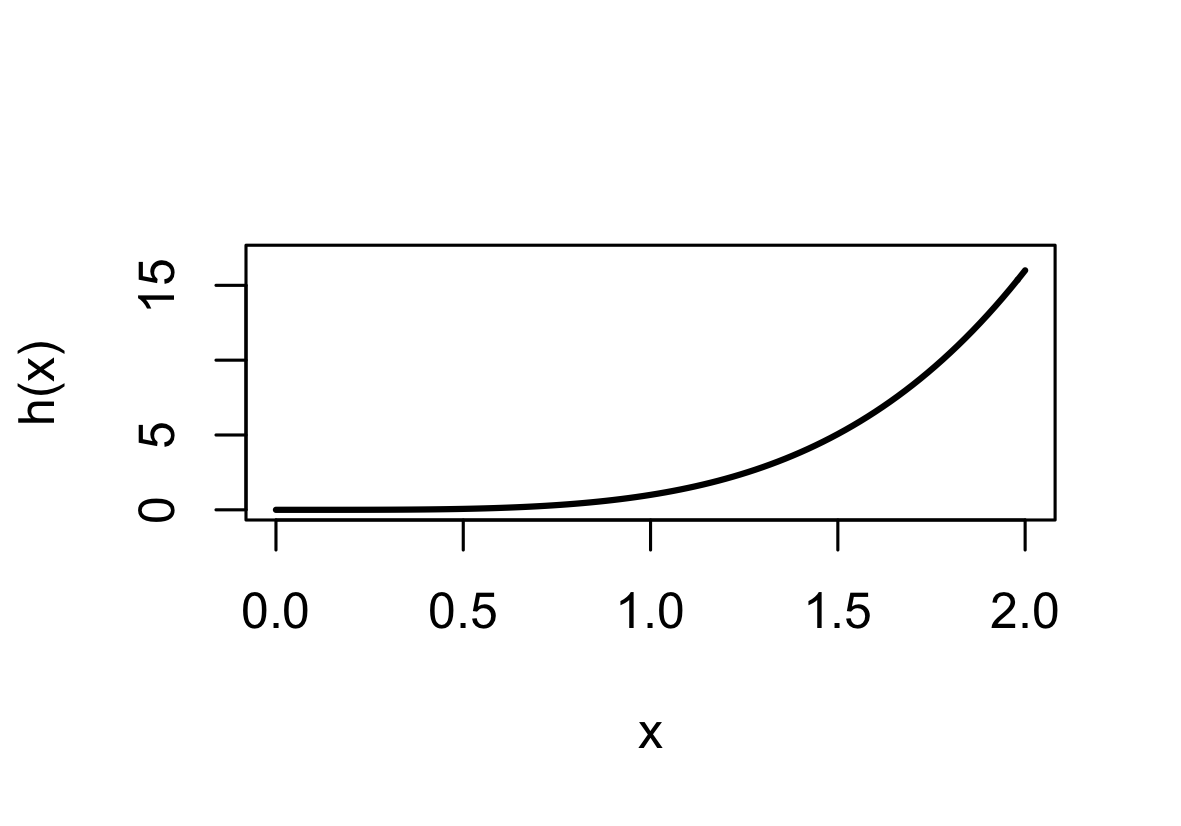
\includegraphics[width=7cm]{hx.png}
\caption{Gráfica de $h(x) = x^4$ para $x\in [0,2]$.}
\label{fig:hx}
\end{figure}

Geométricamente, queremos encontrar el área bajo la curva $h(x) = x^4$ para $0 \leq x \leq 2$. Viendo la figura \ref{fig:hx}, notamos que $\theta$ es una fracción del área del rectángulo $$\mathcal{R} = \left\lbrace (x, y) \in \mathbb{R}^2: 0\leq x \leq 2, \ 0 \leq y \leq 16\right \rbrace,$$ la cual denotaremos $\Theta$. Podemos simular puntos distribuidos de manera uniforme en $\mathcal{R}$. La probabilidad de que uno de estos puntos esté en el área $\Theta$ es $\theta / 32$, donde 32 es el área de $\mathcal{R}.$ Por lo tanto, podemos estimar a $\theta$ utilizando $$\hat{\theta} = \frac{\text{\# de puntos que caen en }\Theta}{\text{\# de puntos simulados}} \times 32.$$

\begin{lstlisting}
y <- runif(nsim, min = 0, max = 16)

exito <- if_else(y <= g(x), 1, 0)

theta_hat2 <- mean(exito) * 32

print(theta_hat2)
print(abs(theta_hat2 - 0.2*32))
\end{lstlisting}

En la figura \ref{fig:sim_hx} se muestran las simulaciones, en azul los puntos que caen en la región $\Theta$ y en gris los demás. Se simularon cien mil puntos y se obtuvo el estimador $\hat{\theta} = 6.42688$, el cual se traduce en un error relativo de 0.42 \% frente al valor real $\theta = 6.4$.

\begin{figure}[H] 
\centering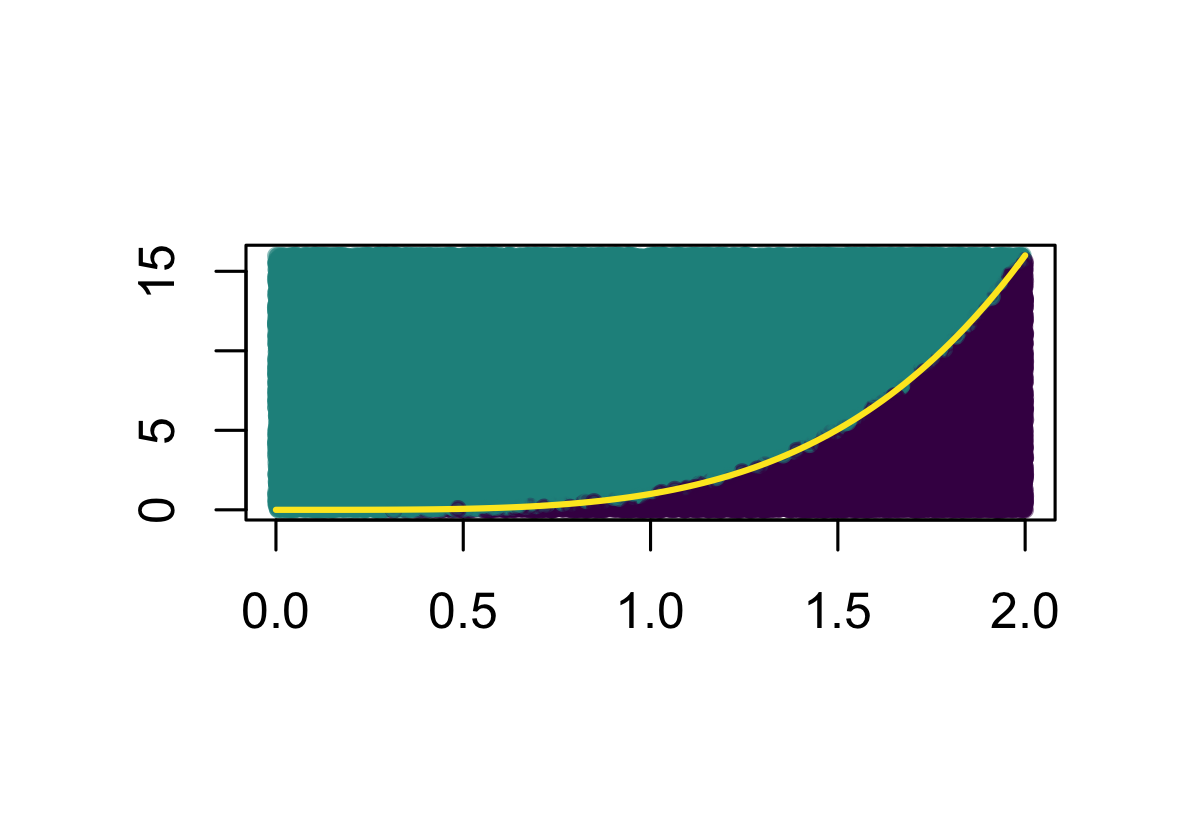
\includegraphics[width=10cm]{sim_hx.png}
\caption{Simulaciones de puntos en el rectángulo $\mathcal{R}$.}
\label{fig:sim_hx}
\end{figure}

La importancia de las técnicas de integración Monte Carlo en el contexto de inferencia estadística recae en que, si tenemos una distribución continua, muchas propiedades de esta distribución se pueden expresar como integrales. Esto es principalmente importante en inferencia bayesiana ya que muchas veces no nos interesa obtener la expresión explícita de las distribuciones posteriores, si no que únicamente queremos su valor esperado.\\

Si tenemos una distribución posterior para $\theta$ de la forma $\theta \sim F(\theta | X_{(n)})$, donde $X_{(n)}$ es una muestra observada de datos, entonces el valor esperado de $\theta| X_{(n)}$ es
\begin{equation}
\label{eq:exp_theta}
E[\theta | X_{(n)}] = \int_{\Theta} \theta \ dF(\theta | X_{(n)}).
\end{equation}
Para calcular esta expresión de manera analítica necesitamos la densidad posterior $$f(\theta | X_{(n)}) = \frac{f(X_{(n)} | \theta)\pi (\theta)}{\int_{\Theta} f(X_{(n)} | \theta)\pi (\theta) \ d\theta}.$$\\

Si el espacio $\Theta$ es de dimensión uno, la integral en el denominador y la integral \eqref{eq:exp_theta} se pueden aproximar con métodos de cuadratura como la regla de Simpson o el método del trapecio (ver \citet{burden}). Sin embargo, a medida que crece la dimensión del espacio parametral, crece también la complejidad de la aproximación con los métodos de cuadratura hasta volverse prácticamente imposible. Es ahí cuando entran las técnicas de integración Monte Carlo. Podemos obtener muestras de la distribución posterior de $\theta$ y aproximar el valor esperado con la media muestral.\\

Cuando la distribución posterior tiene una forma conocida que se puede simular con los métodos del capítulo \ref{simulacion}, entonces la aproximación del valor esperado es directa. En las secciones siguientes veremos qué hacer cuando la distribución posterior no se puede simular con los métodos vistos hasta ahora. La idea de los métodos de cadenas de Markov Monte Carlo es simular cadenas que su distribución estacionaria sea la distribución de interés y utilizar estas simulaciones para la aproximación de la esperanza. Primero se presenta algo de teoría sobre cadenas de Markov.\\

\subsection{Cadenas de Markov}
Esta sección contiene la teoría mínima indispensable de cadenas de Markov para entender los algoritmos MCMC. Es opinión de quien escribe que esta teoría es más comprensible para procesos estocásticos en tiempo discreto y con espacio de estados discreto. Para procesos en tiempo continuo y/o espacio de estados continuo, se recomienda consultar \citet{ross}.\\

\textbf{Definición.} Sea $\lbrace X_t, t \in \mathbb{N}_0\rbrace$ un proceso estocástico con espacio de estados discreto. Se dice que este proceso es una cadena de Markov si 
\begin{align*}
P\lbrace X_{t+1} = j \ | \ X_t = i, X_{t-1} = i_{t-1}, \dots, X_0 = i_0\rbrace &= P\lbrace X_{t+1} = j \ | \ X_t = i\rbrace,
\end{align*}

esto es, \textit{si fijando el presente, el futuro no depende del pasado.}\\

Si $$P\lbrace X_{t+1} = j \ | \ X_t = i\rbrace = P_{ij},$$ independiente de $t$, decimos que la cadena de Markov tiene probabilidades de transición estacionarias. Una cadena de Markov con esta característica se dice que es homogénea. A partir de ahora, haremos referencia únicamente a estas cadenas.\\

\textbf{Definición.} Se define la \textit{probabilidad de transición en n pasos}, denotada $P_{ij}^n$, como
\begin{align*}
P_{ij}^n &= P\lbrace X_{m+n} = j \ | \ X_{m} = i\rbrace\\
&= P\lbrace X_n = j \ | \ X_0 = i \rbrace,
\end{align*}
donde la última igualdad se sigue de la homogeneidad de la cadena.\\

Se dice que el estado $j$ es accesible desde el estado $i$ si existe $n \in \mathbb{N}$ tal que $P_{ij}^n > 0$. Estos dos estados están \textbf{comunicados} si además existe $m \in \mathbb{N}$ tal que $P_{ji}^m > 0$. Que los estados $i$ y $j$ estén comunicados se denota
\begin{equation} \label{clase_eq}
i \leftrightarrow j.
\end{equation}

La comunicación de los estados define una relación de equivalencia (ver \citet{ross}). Así, dos estados comunicados pertenecen a una misma clase de equivalencia. Por las propiedades de estas relaciones, las clases definidas solamente pueden ser iguales o disjuntas. Decimos que una cadena de Markov es \textbf{irreducible} si su espacio de estados cuenta con una única clase de equivalencia.\\

\textbf{Definición.} Definimos el \textit{tiempo de primer regreso al estado i} como $$T_i = \min_{t>0} \lbrace X_0 = i, X_t = i \rbrace.$$\\

Si $P\lbrace T_i < \infty \rbrace = 1 $ entonces decimos que el estado $i$ es \textbf{recurrente}. En otro caso, decimos que el estado $i$ es transitorio. Además, si $i$ es un estado recurrente, decimos que éste es \textbf{recurrente positivo} si $E\left[T_i\right] < \infty$. En otro caso, decimos que $i$ es recurrente nulo.\\

\textbf{Definición.} Definimos el periodo del estado $i$, denotado $d(i)$, como el máximo común divisor de $\lbrace n\in \mathbb{N}: P_{ii}^n > 0\rbrace.$ Si $d(i)=1$, decimos que el estado $i$ es \textbf{aperiódico}.\\

El siguiente resultado muestra que para una cadena de Markov irreducible, si el estado $i$ es recurrente positivo y aperiódico, entonces todos los demás estados también lo son. La demostración se puede consultar en \citep{ross}.

\begin{proposition}
Las propiedades de recurrencia, recurrencia positiva, recurrencia nula y aperiodicidad son comunes a una clase de equivalencia definida por \eqref{clase_eq}.
\end{proposition}

\textbf{Definición.} Decimos que una cadena de Markov es ergódica si es irreducible y todos sus estados son recurrentes positivos y aperiódicos.

\begin{theorem}
Sea $P=[P_{ij}]$ la matriz de transición de una cadena de Markov ergódica. Entonces existe un único vector $\pi = (\pi_1, \pi_2, \dots)^T$ tal que
\begin{equation} \label{dist_limite}
\lim_{n \to \infty}P^n = [\pi \ \pi \dots \pi \dots ]^T.
\end{equation}
A $\pi$ se le conoce como la \textbf{distribución estacionaria} de la cadena ergódica.
\end{theorem}

Si queremos obtener muestras de una densidad $f$, difíciles o imposibles de obtener con los métodos mencionados en la sección \ref{simulacion}, la idea de los algoritmos de MCMC es crear una cadena de Markov ergódica cuya distribución estacionaria sea $f$ y simular observaciones de esta cadena. En el límite, estas observaciones siguen una distribución dada por $f$.\\

Recordemos que en esta sección presentamos las ideas únicamente con cadenas de Markov con espacio de estados discreto. Sin embargo algunas propiedades como la irreducibilidad, aperiodicidad, la recurrencia y la existencia de una distribución estacionaria se pueden trasladar a cadenas con espacio de estados continuo, que son las que utilizaremos en las secciones siguientes. En el caso continuo, en vez de contar con una matriz de transición, se tiene un \textit{kernel} de transición. El kernel de transición, denotado $P(x, \mathcal{A})$, es una función de distribución condicional que representa la probabilidad de moverse de $x$ a un punto en el conjunto $\mathcal{A}$ \citep{chib_mh}.\\

\subsection{Muestreador de Gibbs}
En las siguientes dos secciones se introducen dos de los algoritmos más importantes de cadenas de Markov Monte Carlo, el muestreador de Gibbs y el algoritmo de Metropolis-Hastings. Aunque el muestredor de Gibbs es un caso especial del algoritmo de Metropolis-Hastings, vamos a hablar antes del primero porque el algoritmo de Metropolis-Hastings había vivido en las tinieblas hasta la aparición del muestreador de Gibbs.\\

Antes de explicar cómo funciona el muestreador de Gibbs, situémonos en el contexto histórico en el que apareció para poder entender la importancia que representó su invención. Este contexto está completamente basado en el libro \textit{The Theory That Would Not Die} de Sharon Bertsch, una lectura obligada para todo aquel interesado en el desarrollo histórico de la estadística bayesiana.\\

Para 1980, las bases teóricas de la inferencia bayesiana estaban bien establecidas y desarrolladas por estadísticos como Leonard Jimmie Savage, Bruno de Finetti y Dennis Lindley. Sin embargo, el uso de estas técnicas estaba limitado por la dificultad de realizar todos los cálculos a mano. Las primeras computadoras hacían que la información fuera más accesible, pero esto a su vez hizo que creciera la dimensión de los espacios parametrales de interés, por lo que resultaba prácticamente imposible estudiar distribuciones a priori, verosimilitudes y distribuciones posteriores en estos espacios.\\

El muestreador de Gibbs \textit{(Gibbs sampler)} fue introducido por los hermanos Stuart y Donald Geman como una herramienta para el reconocimiento de imágenes en 1984. A pesar de esto, tampoco fue muy utilizado en la práctica ya que el gran número de pixeles en una imagen era inmanejable para las computadoras de la época. Algún tiempo después se supo que el matemático ruso Valentin Fedorovich Turchin había descubierto el muestreador de Gibbs en 1971 pero su artículo solamente apareció en publicaciones rusas y no tuvo gran difusión \citep{bertsch}.\\

La aparición del muestreador de Gibbs como un método de simulación se debe a Alan Gelfand y Adrian F. M. Smith. En su artículo \textit{Sampling-Based Approaches to Calculating Marginal Densities}, publicado en 1990, los autores explican el uso del algoritmo de los hermanos Geman para obtener muestras de distribuciones marginales a partir de distribuciones condicionales. Alan Gelfand explicó que el muestreador de Gibbs toma el problema de simular observaciones de una distribución de gran dimensión y lo divide en pequeños pedazos que son fáciles de resolver \citep{bertsch}. Estos pedazos son obtener muestras de distribuciones condicionales. Veamos ahora cómo se hace esto y por qué funciona.\\

Pensemos primero en un caso con dos variables aleatorias, $X$ y $Y$. La idea del muestreador de Gibbs es simular observaciones de las distribuciones marginales $f_X$ y $f_Y$ utilizando simulaciones de las distribuciones condicionales $f_{X|Y}$ y $f_{Y|X}$, suponiendo que estas condicionales son conocidas y fáciles de simular.\\

El algoritmo en el caso bivariado es como sigue. Primero se fijan valores iniciales $X^{(0)}, Y^{(0)}$. Luego en la iteración $t$:
\begin{enumerate}
\item Simular $Y^{(t)} \sim Y|X = x^{(t-1)}$.
\item Simular $X^{(t)} \sim X|Y = y^{(t)}$.
\end{enumerate}

Como se menciona en \citet{casella_gs}, bajo ciertas condiciones generales la distribución de la sucesión $\lbrace X_t \rbrace$ converge a la distribución marginal $f_X$. De la misma manera, la distribución del proceso $\lbrace Y_t \rbrace$ converge a la distribución $f_Y$.\\

Para ilustrar el algoritmo presentamos un ejemplo que aparece en \citet{casella}. Tenemos que el vector $(X, Y)$ tiene una distribución normal bivariada con vector de medias $\mu = [0, 0]^T$ y matriz de covarianza $\big(\begin{smallmatrix}
  1 & 0.8\\
  0.8 & 1
\end{smallmatrix}\big)$. Así, marginalmente se cumple que $X \sim \mathcal{N}(0, 1)$ y $Y \sim \mathcal{N}(0, 1)$. Simularemos de estas distribuciones utilizando el muestreador de Gibbs. Para esto, necesitamos las distribuciones condicionales, las cuales están dadas por $$Y|X = x \sim \mathcal{N}(\rho x, 1 - \rho^2)$$ y $$X|Y = y \sim \mathcal{N}(\rho y, 1 - \rho^2).$$\\

Establecemos los valores iniciales $X^{(0)}, Y^{(0)}$ y corremos el algoritmo por 10 mil iteraciones. En la figura \ref{fig:gs_norm} graficamos las distribuciones marginales, comparándolas contra la densidad normal estándar verdadera y vemos la correlación con un diagrama de dispersión. El código para generar las simulaciones es el siguiente.\\

\begin{lstlisting}
nsim <- 1e4

x <- vector(mode = "double", length = nsim)
y <- vector(mode = "double", length = nsim)

set.seed(42)

x[1] <- rnorm(1)
y[1] <- rnorm(1)

rho <- 0.8

for (i in 1:(nsim - 1)) {
  y[i + 1] <- rnorm(1, mean = rho * x[i], sd = sqrt((1 - rho^2)))
  x[i + 1] <- rnorm(1, mean = rho * y[i + 1], sd = sqrt((1 - rho^2)))
}
\end{lstlisting}

\begin{figure}
    \centering
    \begin{subfigure}[t]{0.45\textwidth}
        \centering
        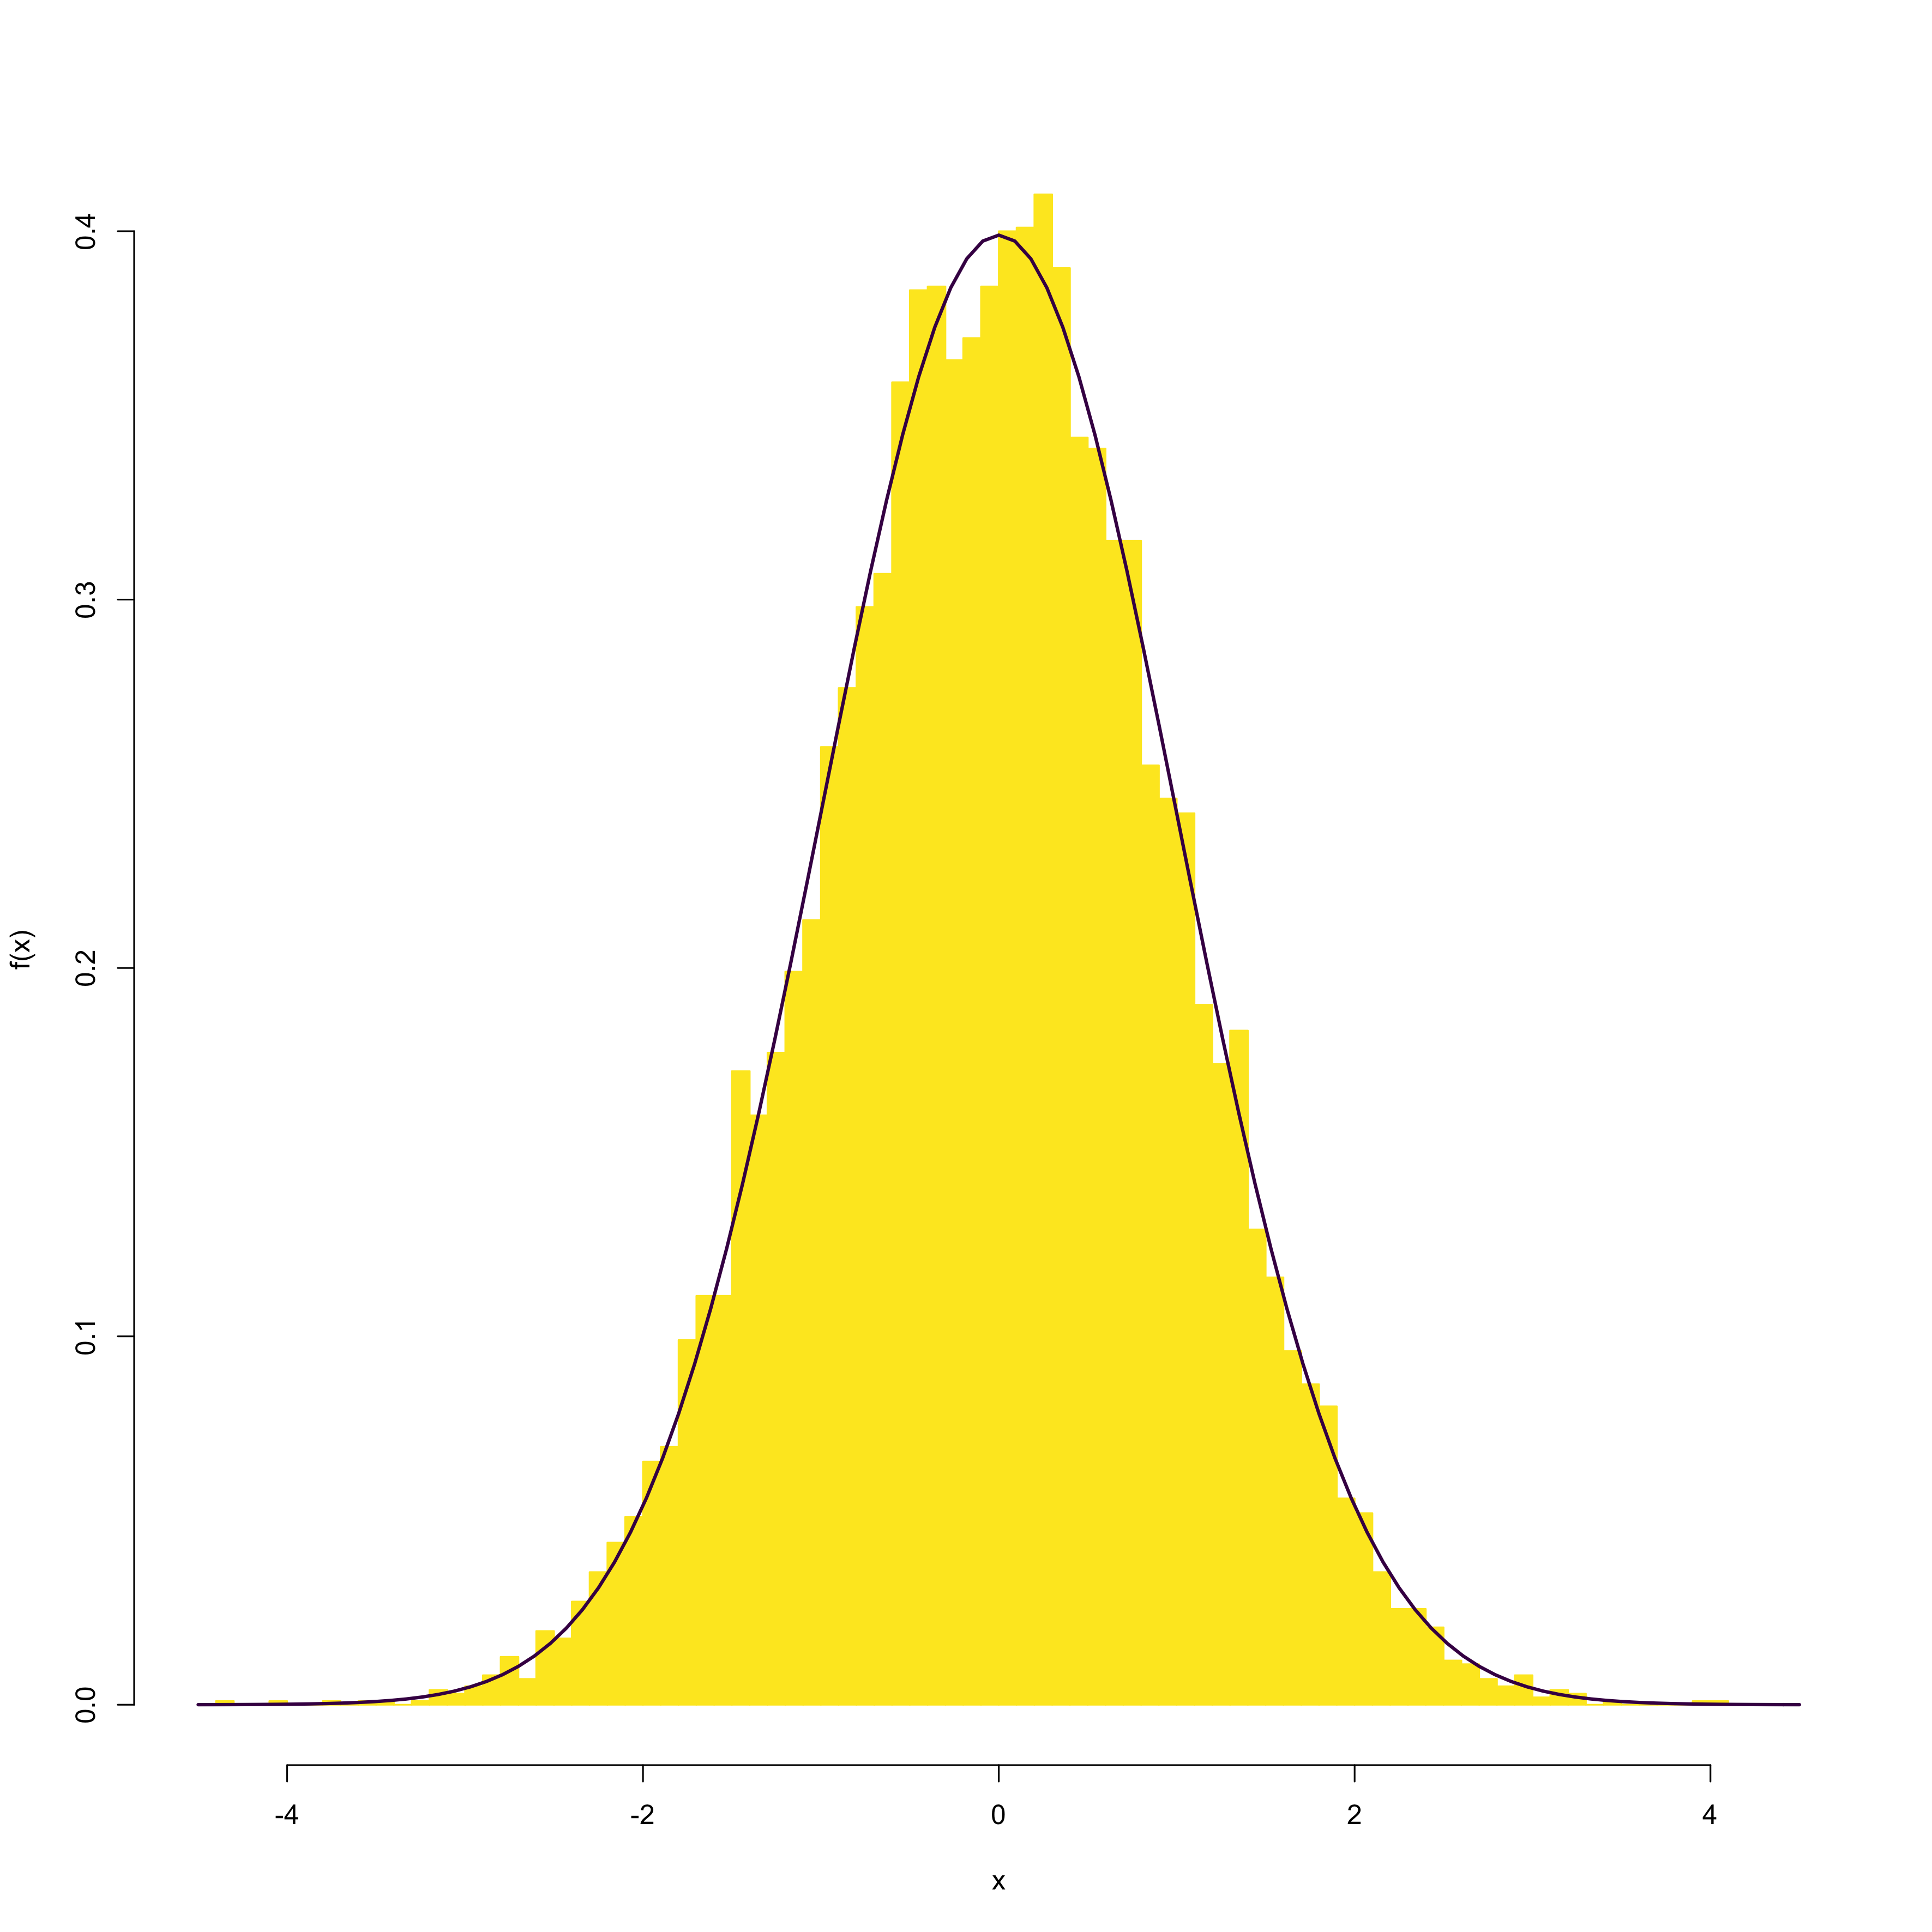
\includegraphics[width=\linewidth]{x_norm.png} 
        \caption{Distribución marginal $f_X$.} \label{fig:xnorm}
    \end{subfigure}
    \hfill
    \begin{subfigure}[t]{0.45\textwidth}
        \centering
        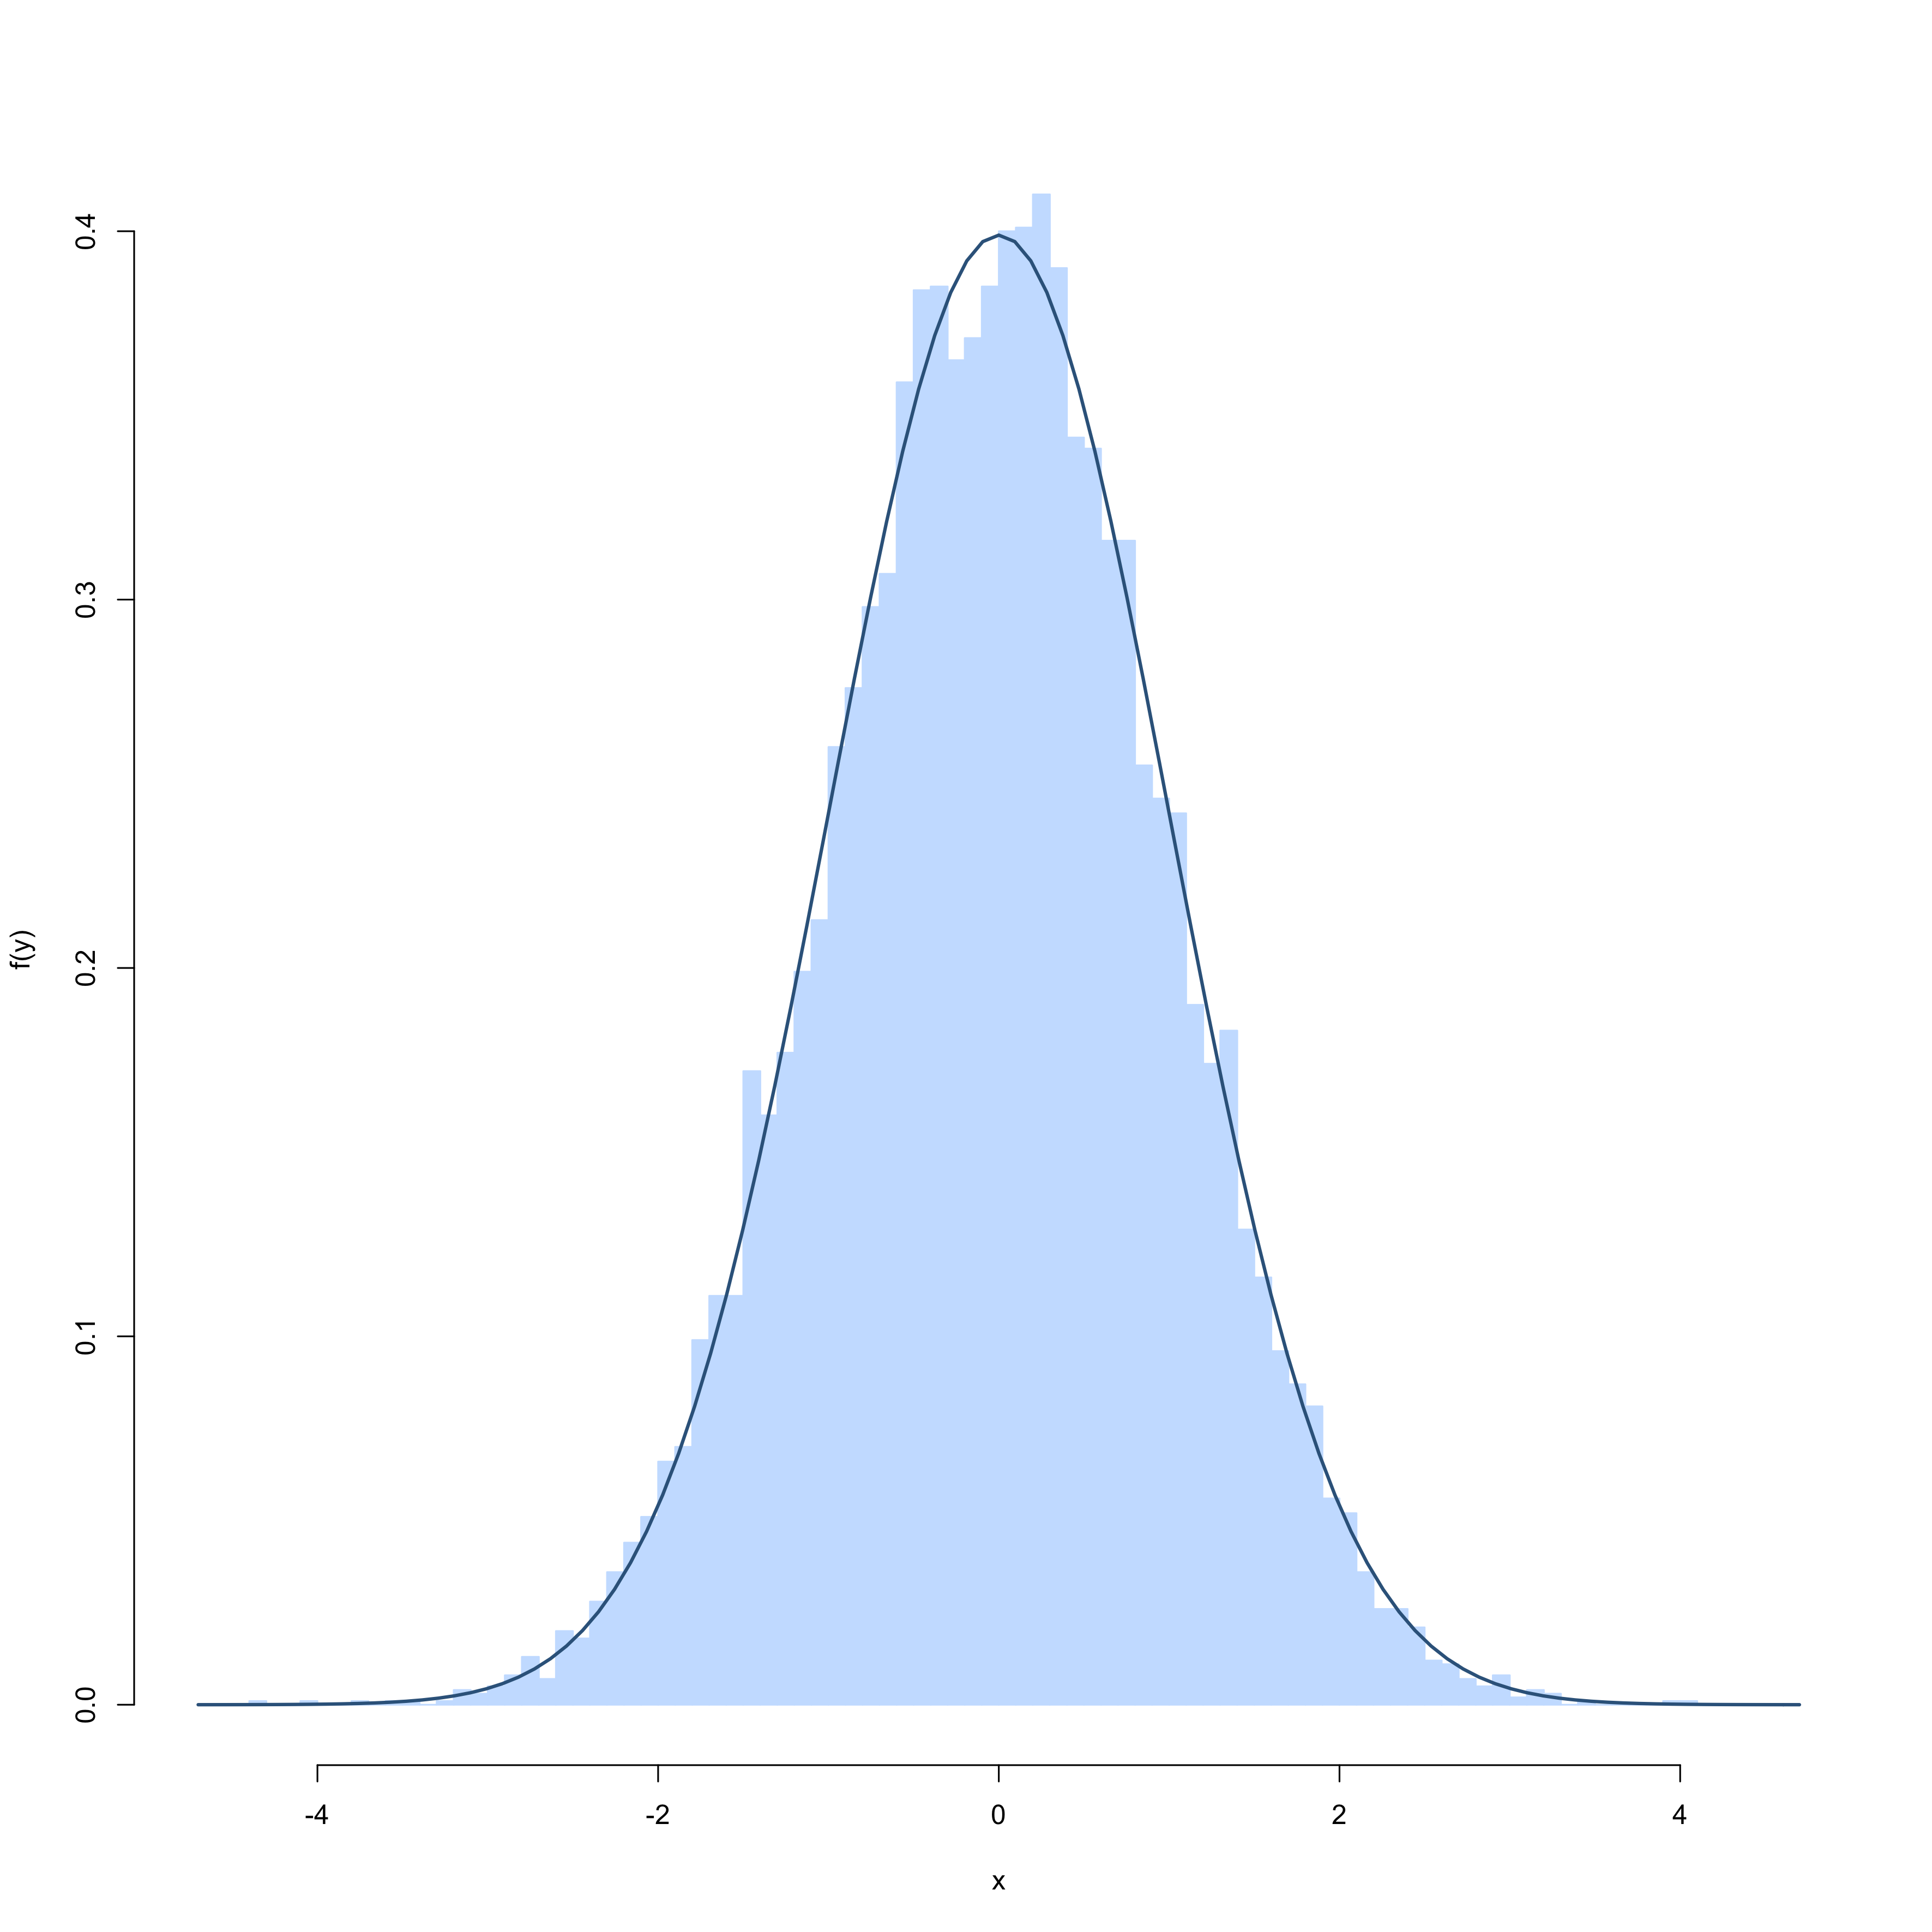
\includegraphics[width=\linewidth]{y_norm.png} 
        \caption{Distribución marginal $f_Y$.} \label{fig:ynorm}
    \end{subfigure}

    \vspace{0.2cm}
    \begin{subfigure}[t]{\textwidth}
    \centering
        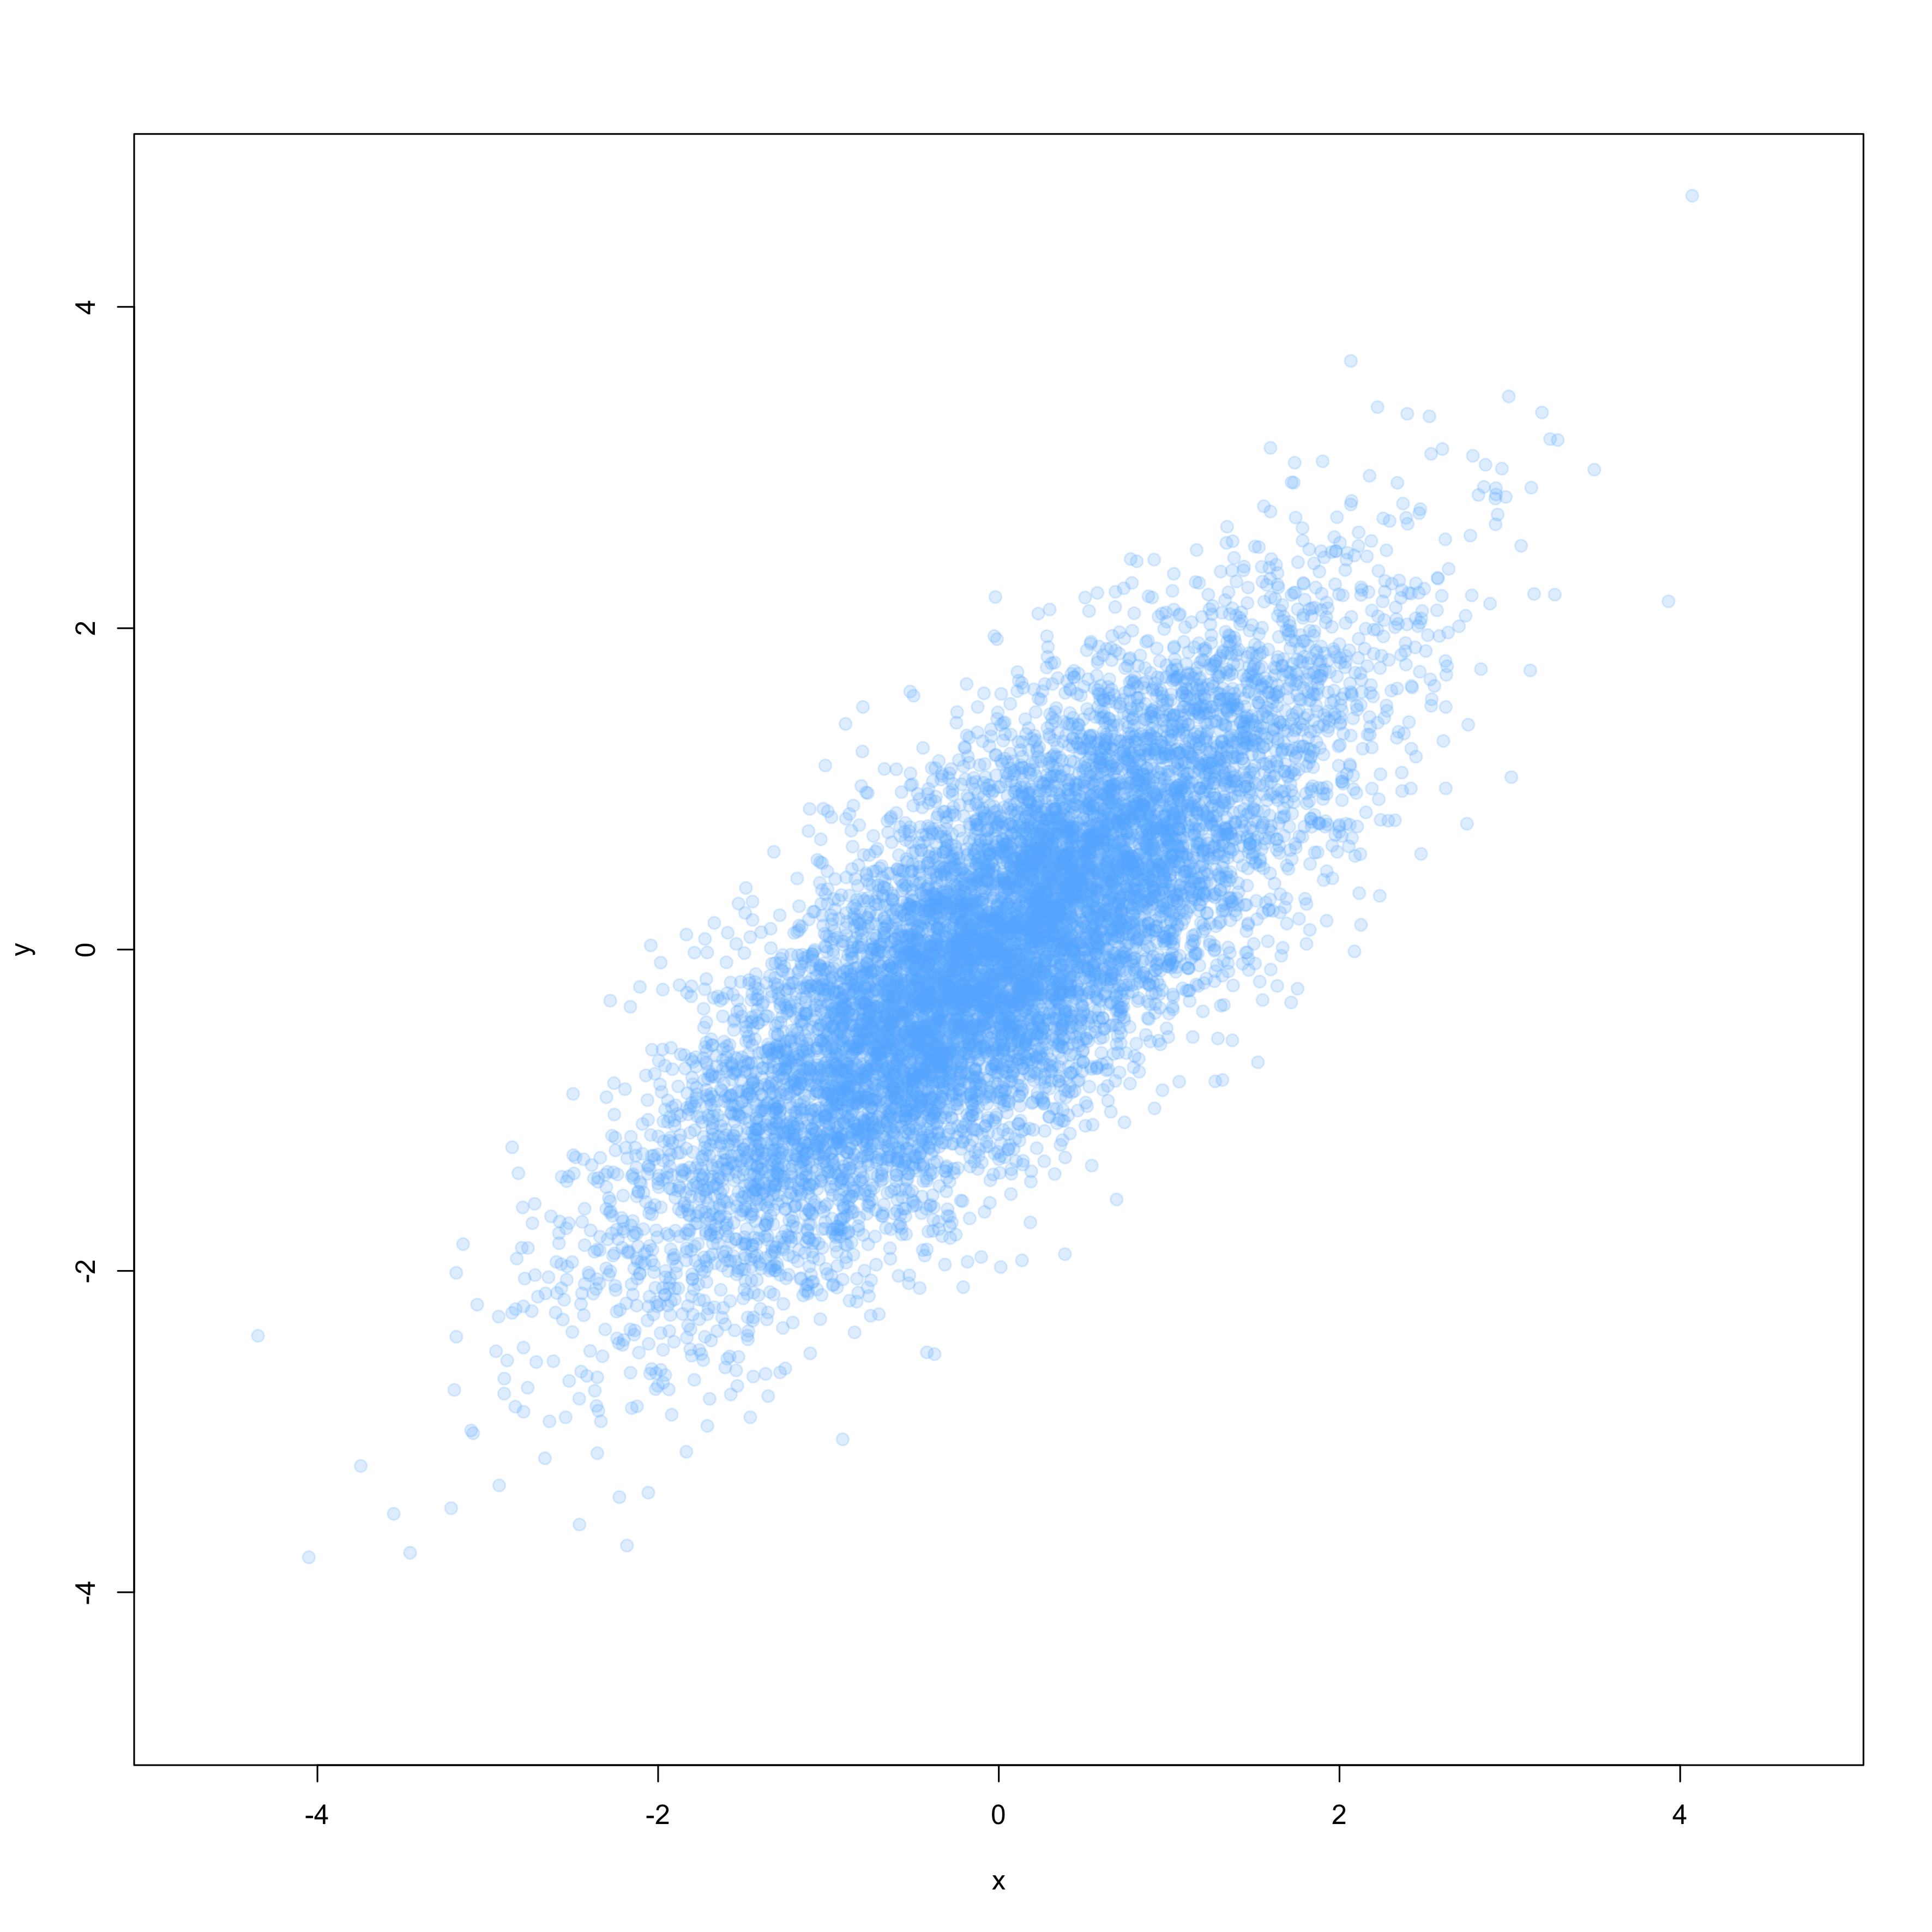
\includegraphics[width=9cm]{bivnorm.png} 
        \caption{Diagrama de dispersión de $(X, Y)$.} \label{fig:bivnorm}
    \end{subfigure}
    \caption{Simulación de un vector normal utilizando el muestreador de Gibbs.}
    \label{fig:gs_norm}
\end{figure}

Como se puede ver en los páneles \ref{fig:xnorm} y \ref{fig:ynorm} de la figura \ref{fig:gs_norm}, las distribuciones marginales empíricas de los procesos $\lbrace X_t \rbrace$ y $\lbrace Y_t \rbrace$ son muy similares a las de una normal estándar, mientras que el diagrama de dispersión \ref{fig:bivnorm} muestra la forma elíptica característica de una distribución normal bivariada con componentes correlacionadas.\\

La extensión del muestreador de Gibbs a mayores dimensiones se hace de la misma manera. Supongamos que tenemos un vector aleatorio $\theta$, dividido en $p$ subvectores $\theta = (\theta_1, \theta_2, \dots, \theta_p)$. Si conocemos todas las distribuciones condicionales de la forma $f_{\theta_i | \theta_{-i}},$ $i \in \lbrace 1, 2, \dots, p\rbrace$ entonces podemos simular observaciones de las densidades marginales con el siguiente algoritmo. Primero establecemos valores iniciales $\theta^{(0)} = (\theta_1^{(0)}, \theta_2^{(0)}, \dots, \theta_p^{(0)})$. Luego, la iteración $t$ del algoritmo es:

\begin{itemize}
\item[] 1. Simular $\theta_1^{(t)} | \theta_2^{(t-1)}, \dots, \theta_p^{(t-1)}$
\item[] 2. Simular $\theta_2^{(t)} | \theta_1^{(t)}, \theta_3^{(t-1)}, \dots, \theta_p^{(t-1)}$
\item[] $\dots$
\item[] p. Simular $\theta_p^{(t)} | \theta_1^{(t)}, \theta_2^{(t)}, \dots, \theta_{p-1}^{(t)}$
\end{itemize}

En \citet{geman} se muestran las condiciones bajo las cuales la distribución del proceso $\lbrace (\theta_1, \theta_2, \dots, \theta_p)_t\rbrace$ converge a la distribución conjunta $f_{\theta}$ \textbf{sin importar los valores iniciales} y por lo tanto, la distribución del proceso $\lbrace \theta_i^t \rbrace$ converge a la distribución marginal $f_{\theta_i}$ \citep{gelfand_smith}. Para estudiar las propiedades matemáticas de esta convergencia, es opinión de quien escribe que resulta más sencillo comprender las propiedades del algoritmo de Metropolis-Hastings y entender el muestreador de Gibbs como un caso particular de éste. Es importante notar que si los subvectores en que dividimos el vector $\theta$ son en realidad cada uno de sus elementos, entonces todas las simulaciones que debemos realizar en el algoritmo son de distribuciones univariadas, lo cual suele simplificar la programación.\\

Una de las mayores facilidades del muestreador de Gibbs es que es común encontrar la especificación de distribuciones conjuntas a través de las condicionales cuando se trabaja con modelos jerárquicos. Esto es ejemplificado por diversos autores como \citet{casella}, \citet{gelman} y \citet{gelfand_smith}. Otra ventaja que señalan \citet{casella} es que el muestreador de Gibbs se puede utilizar para trabajar con modelos de variables latentes. Estos son modelos expresados de la forma $$f(x| \theta) = \int_\Xi f(x, \xi | \theta) \ d\xi,$$ donde $\xi$ es la variable latente (no observable) y $\Xi$ su soporte. En la sección \ref{elmodelo} se utilizan estos modelos para describir la correlación entre tiempos de fallo y para trabajar con observaciones no exactas.\\

Se presenta un ejemplo de un modelo jerárquico para ilustrar el muestreador de Gibbs con más de dos variables \citep{casella_gs}. La especificación del modelo es como sigue.
\begin{itemize}
\item $\omega|\theta, \gamma \sim Binomial(\gamma, \theta)$
\item $\theta | \omega, \gamma \sim Be(\omega + \alpha, \gamma - \omega + \beta)$
\item $\gamma | \omega, \theta \propto e^{-\lambda(1-\theta)}\frac{[(1-\theta)\lambda]}{(\gamma - \omega)!}^{\gamma - \omega},$
\end{itemize}
donde $\alpha$, $\beta$ y $\lambda$ son hiperparámetros constantes. La distribución condicional $\gamma | \omega, \theta$ es una Poisson con parámetro $\lambda(1-\theta)$ y el soporte desplazado a $[\omega, \infty)$. Para obtener muestras de esta distribución podemos simular $\delta \sim Po(\lambda(1-\theta))$ y hacer $\gamma = \delta + \omega$. Primero, tomamos los valores iniciales $\omega^{(0)}$, $\theta^{(0)}$ y $\gamma^{(0)}$. A continuación se incluye el códgio para realizar las simulaciones. Utilizamos los valores de los hiperparámetros $\alpha = 2$, $\beta = 4$ y $\lambda = 16$ y realizamos 10 mil iteraciones.\\

\begin{lstlisting}
set.seed(42)
nsim <- 1e4

alpha <- 2
beta <- 4
lambda <- 16

omega <- vector(mode = "double", length = nsim)
gamma <- vector(mode = "double", length = nsim)
theta <- vector(mode = "double", length = nsim)

omega[1] <- rbinom(n = 1, size = 5, prob = 0.5)
theta[1] <- rbeta(n = 1, shape1 = alpha, shape2 = beta)
gamma[1] <- rpois(n = 1, lambda = 4) + omega[1]

for (i in 2:nsim) {
  omega[i] <- rbinom(n = 1, size = gamma[i - 1], prob = theta[i - 1])
  theta[i] <- rbeta(
    n = 1,
    shape1 = omega[i] + alpha,
    shape2 = gamma[i - 1] - omega[i] + beta
    )
  gamma[i] <- omega[i] + rpois(n = 1, lambda = lambda * (1 - theta[i]))
}
\end{lstlisting}

\begin{figure}
    \centering
    \begin{subfigure}[t]{0.45\textwidth}
        \centering
        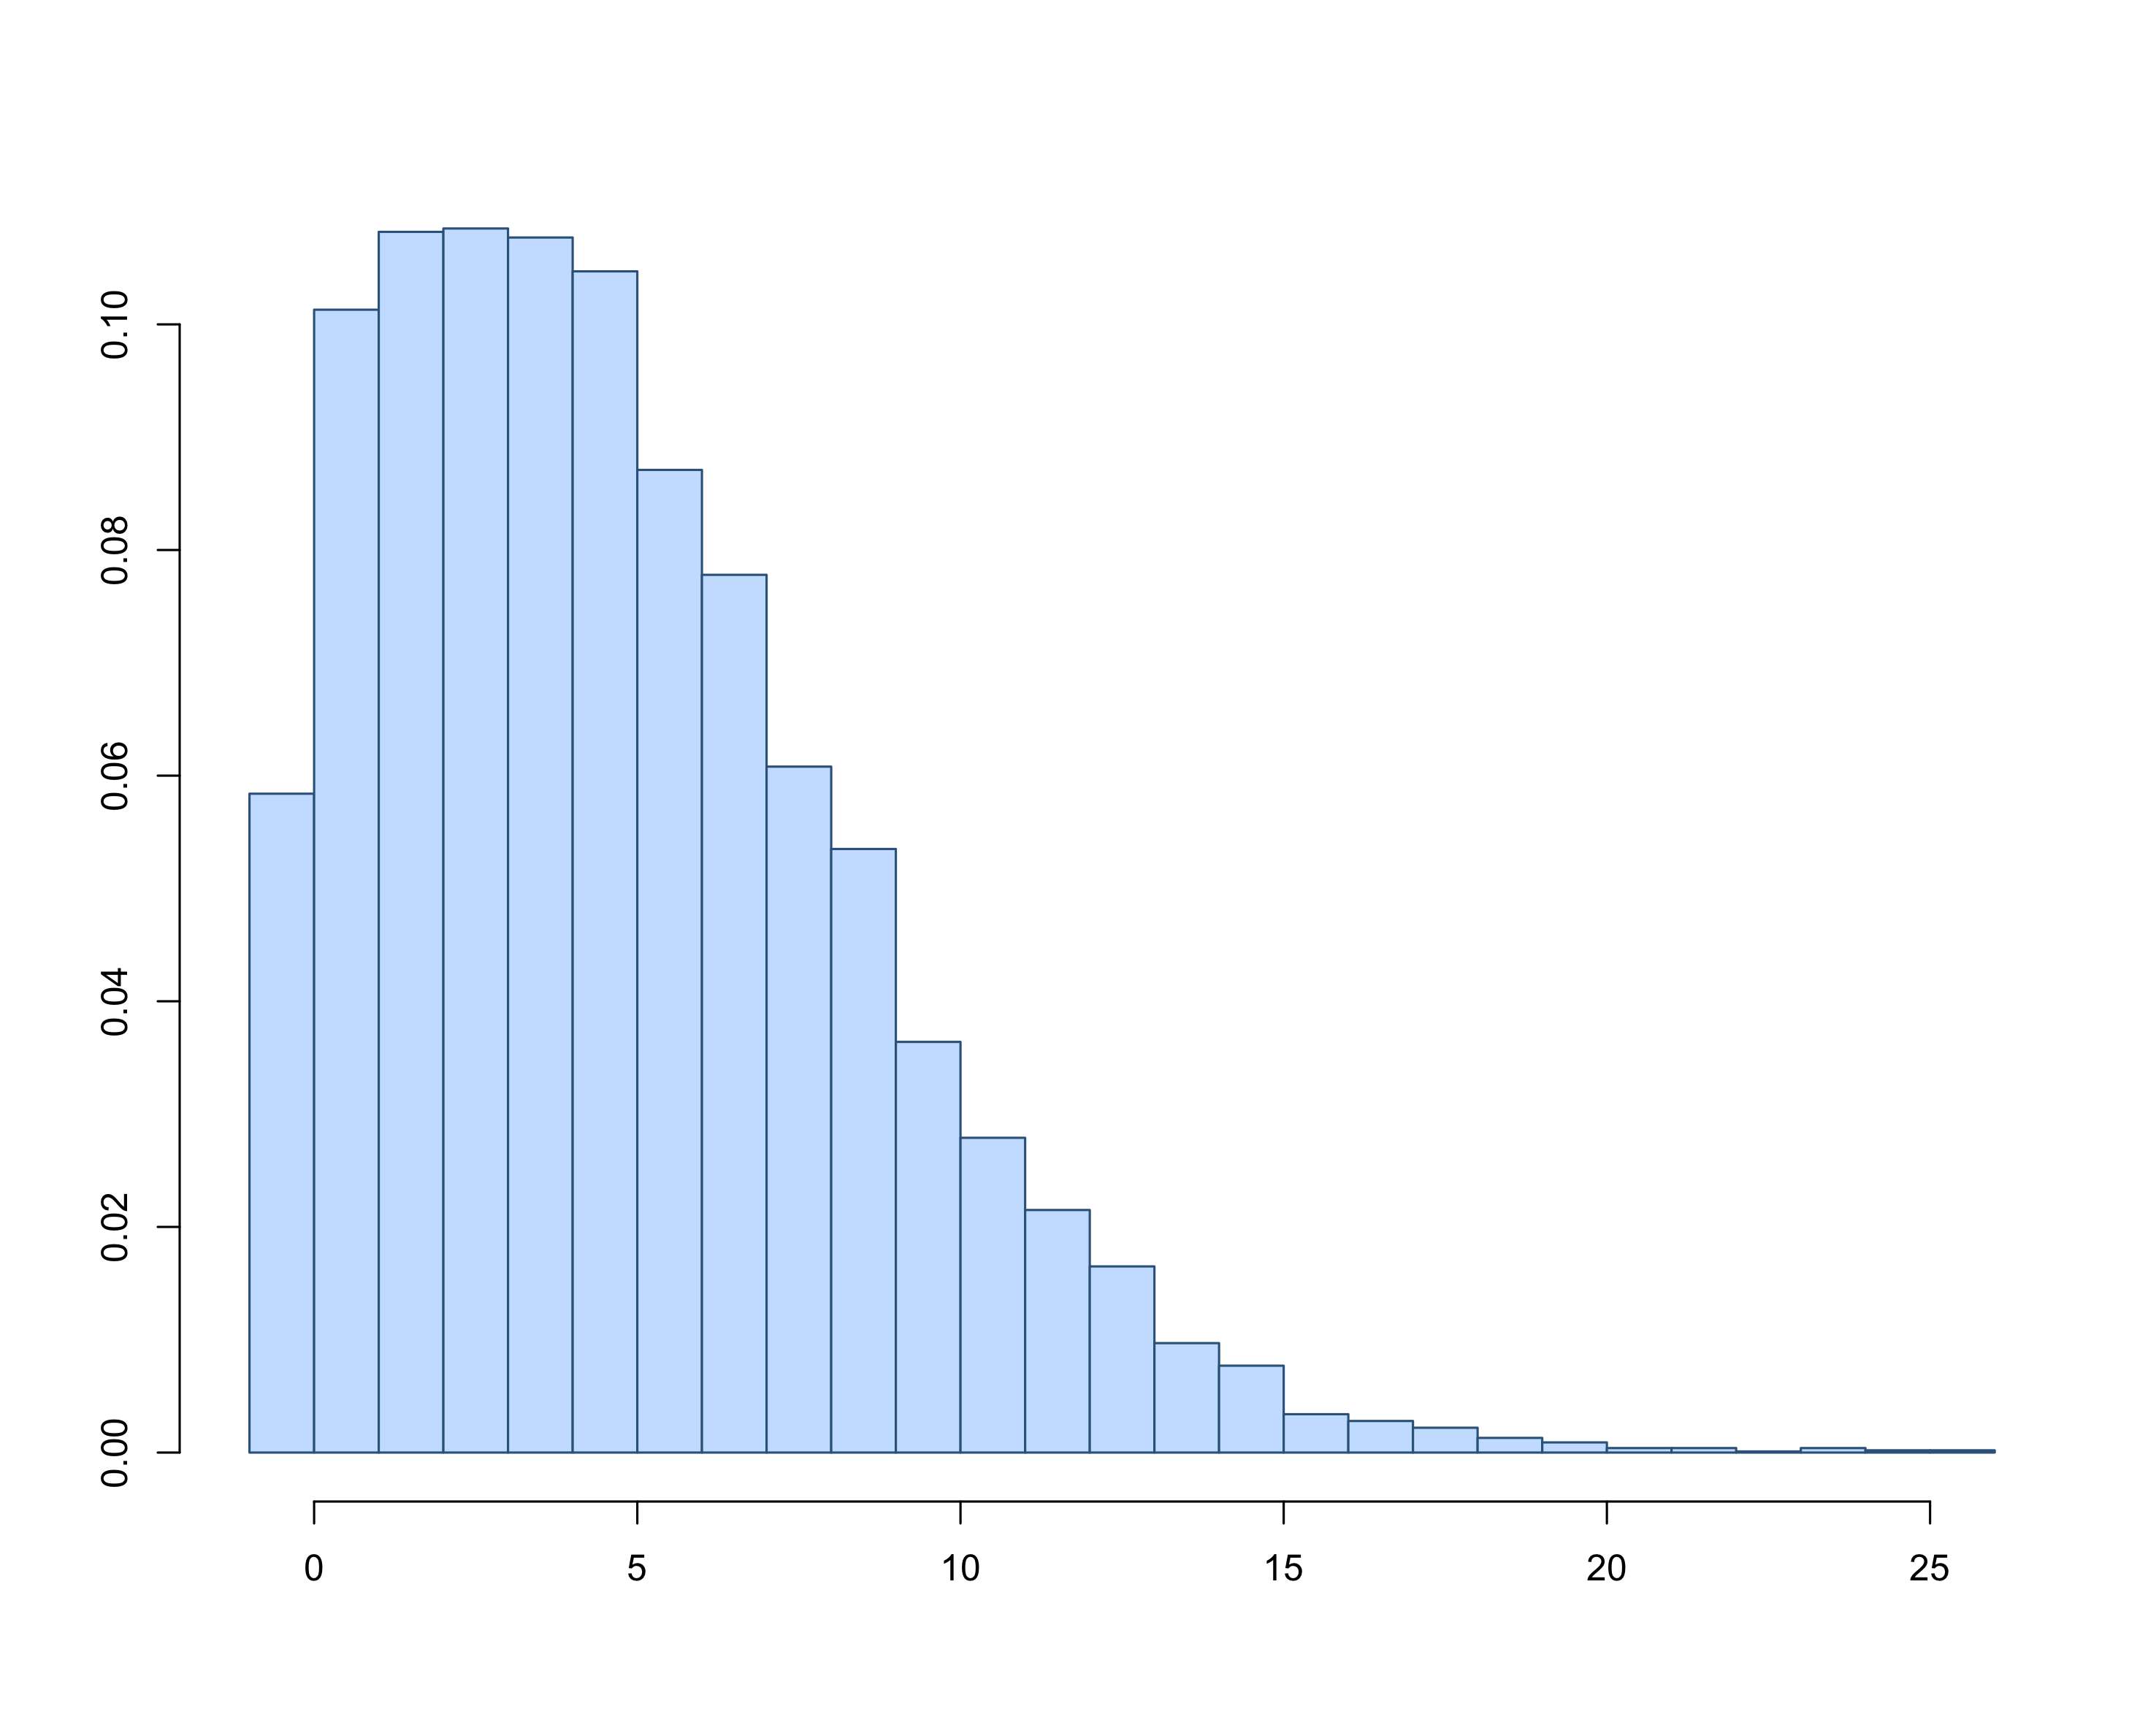
\includegraphics[width=\linewidth]{hier_hist_omega.png} 
        \caption{Distribución marginal $f_\omega$.} \label{fig:hier_hist_omega}
    \end{subfigure}
    \hfill
    \begin{subfigure}[t]{0.45\textwidth}
        \centering
        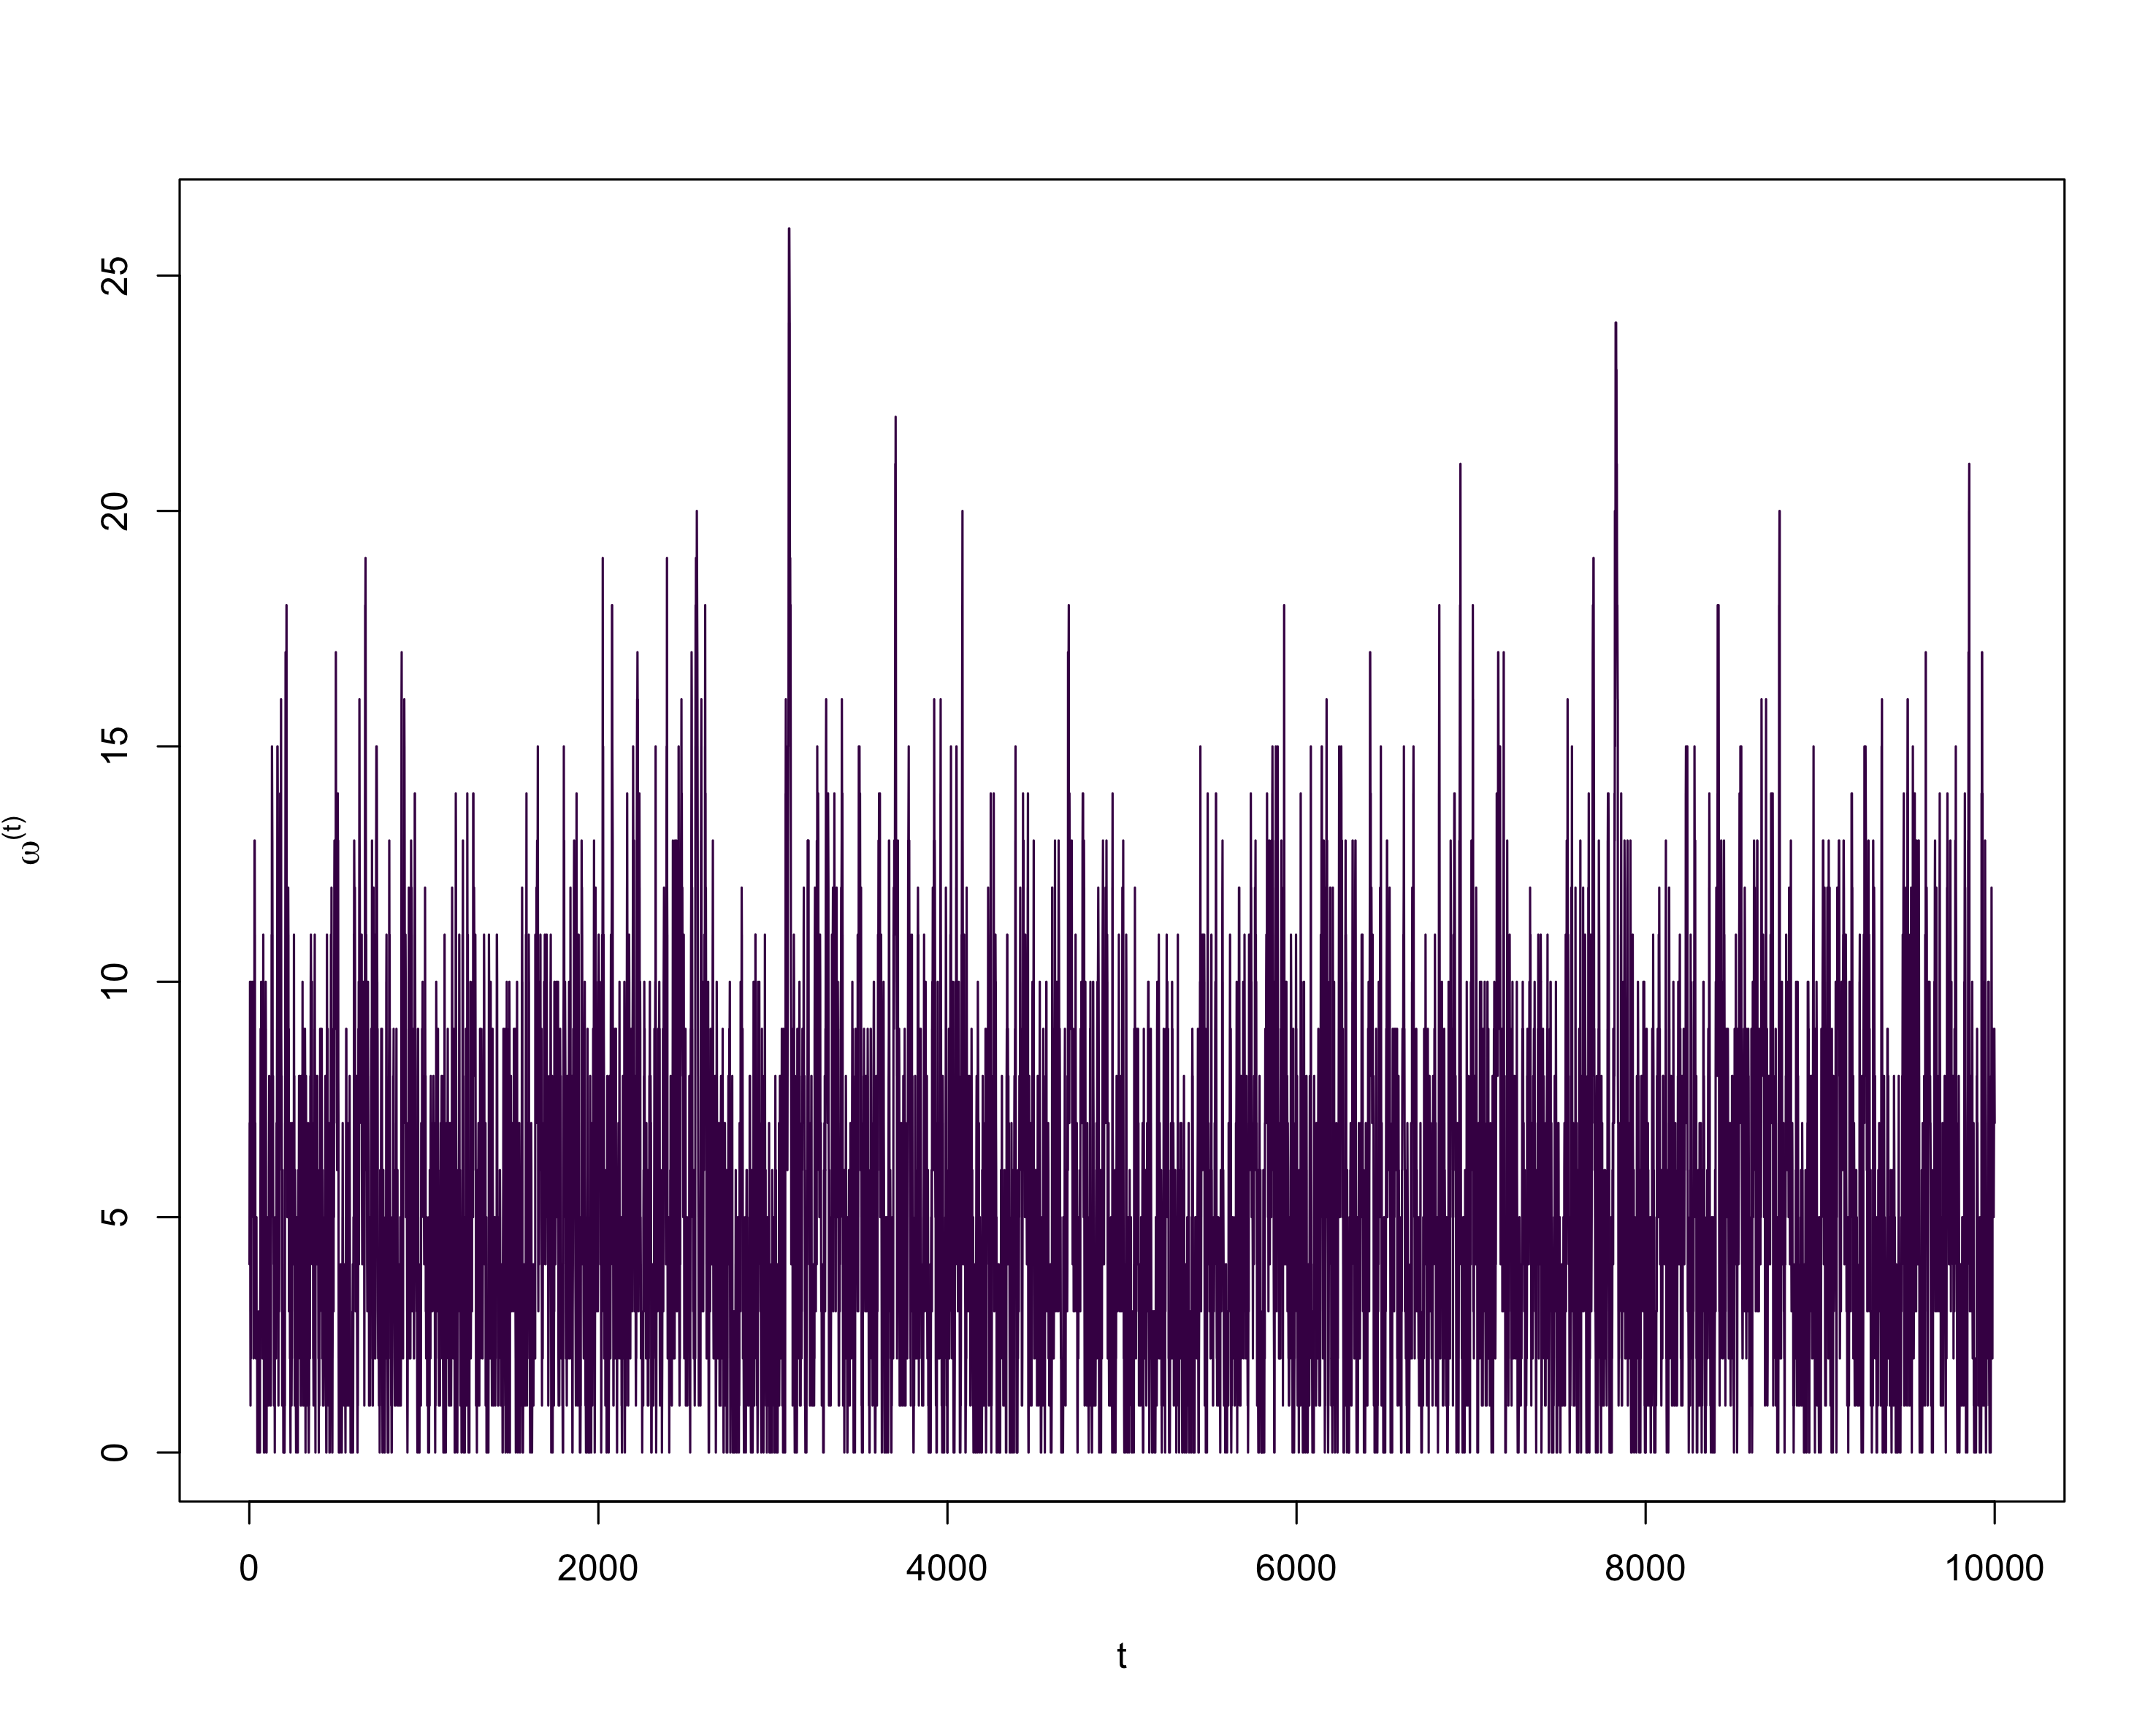
\includegraphics[width=\linewidth]{hier_chain_omega.png} 
        \caption{Proceso $\lbrace \omega_t \rbrace$} \label{fig:hier_chain_omega}
    \end{subfigure}

    \vspace{0.2cm}
    
    \begin{subfigure}[t]{0.45\textwidth}
        \centering
        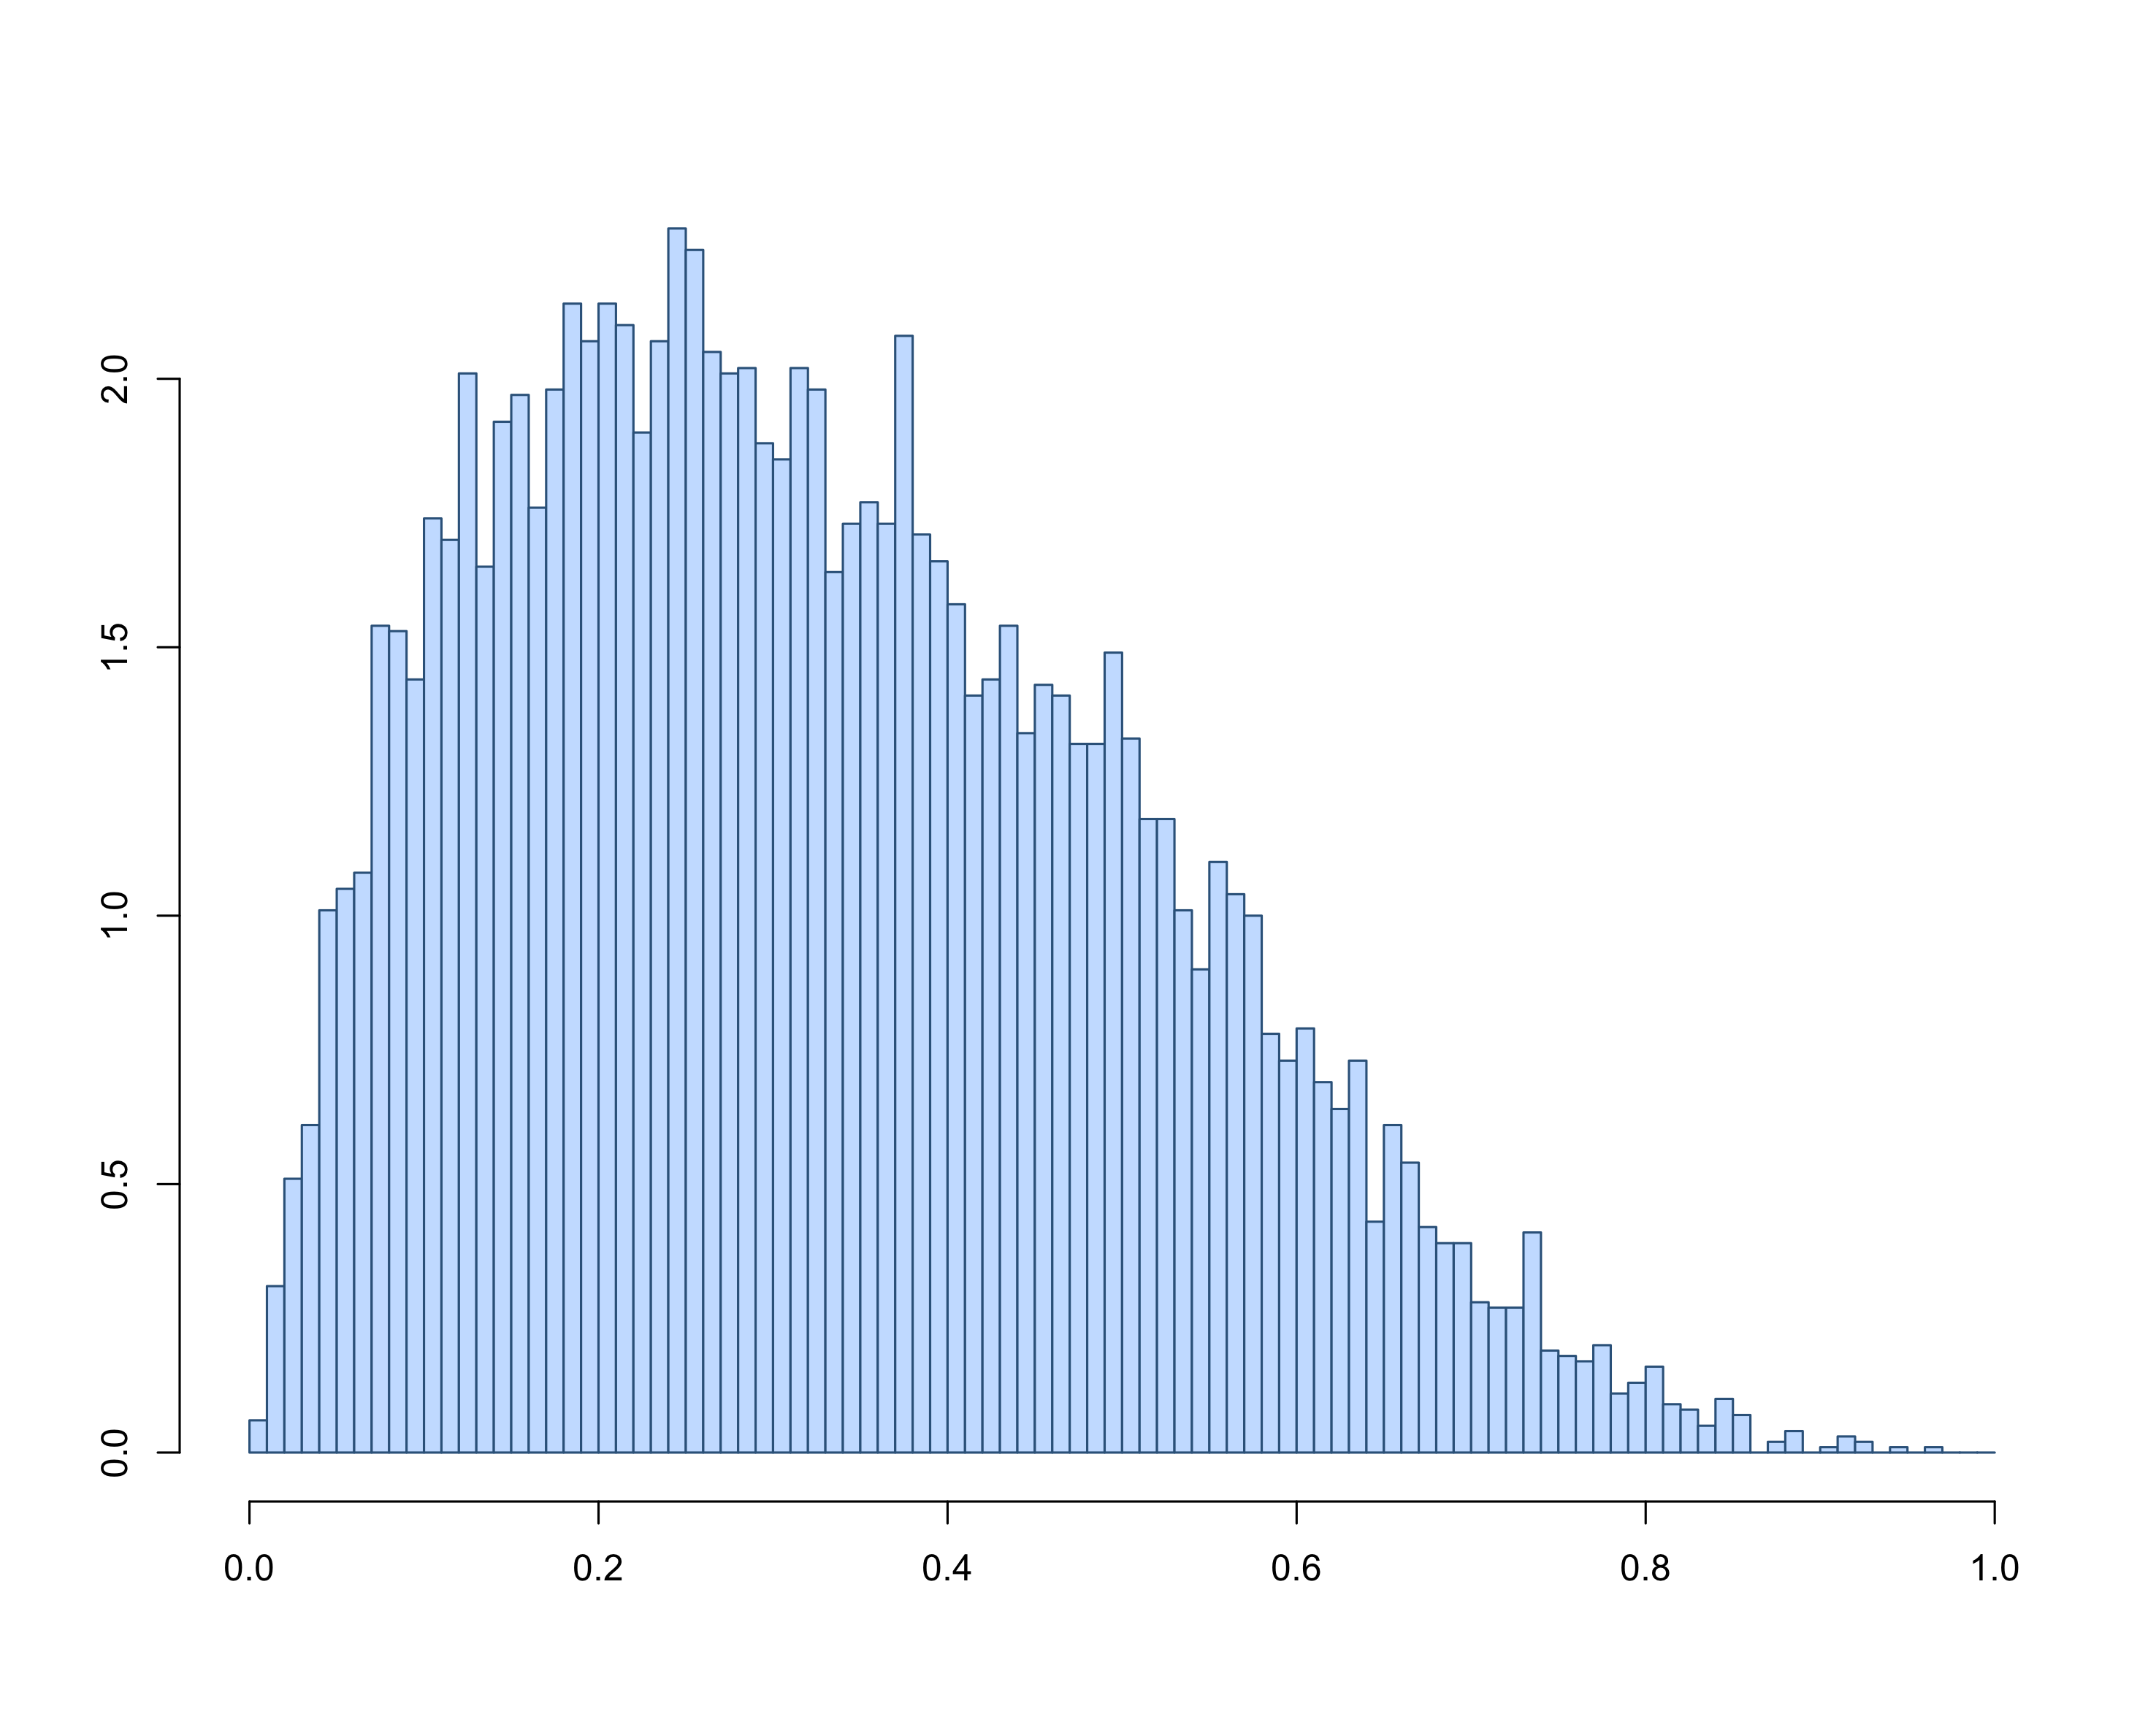
\includegraphics[width=\linewidth]{hier_hist_theta.png} 
        \caption{Distribución marginal $f_\theta$.} \label{fig:hier_hist_theta}
    \end{subfigure}
    \hfill
    \begin{subfigure}[t]{0.45\textwidth}
        \centering
        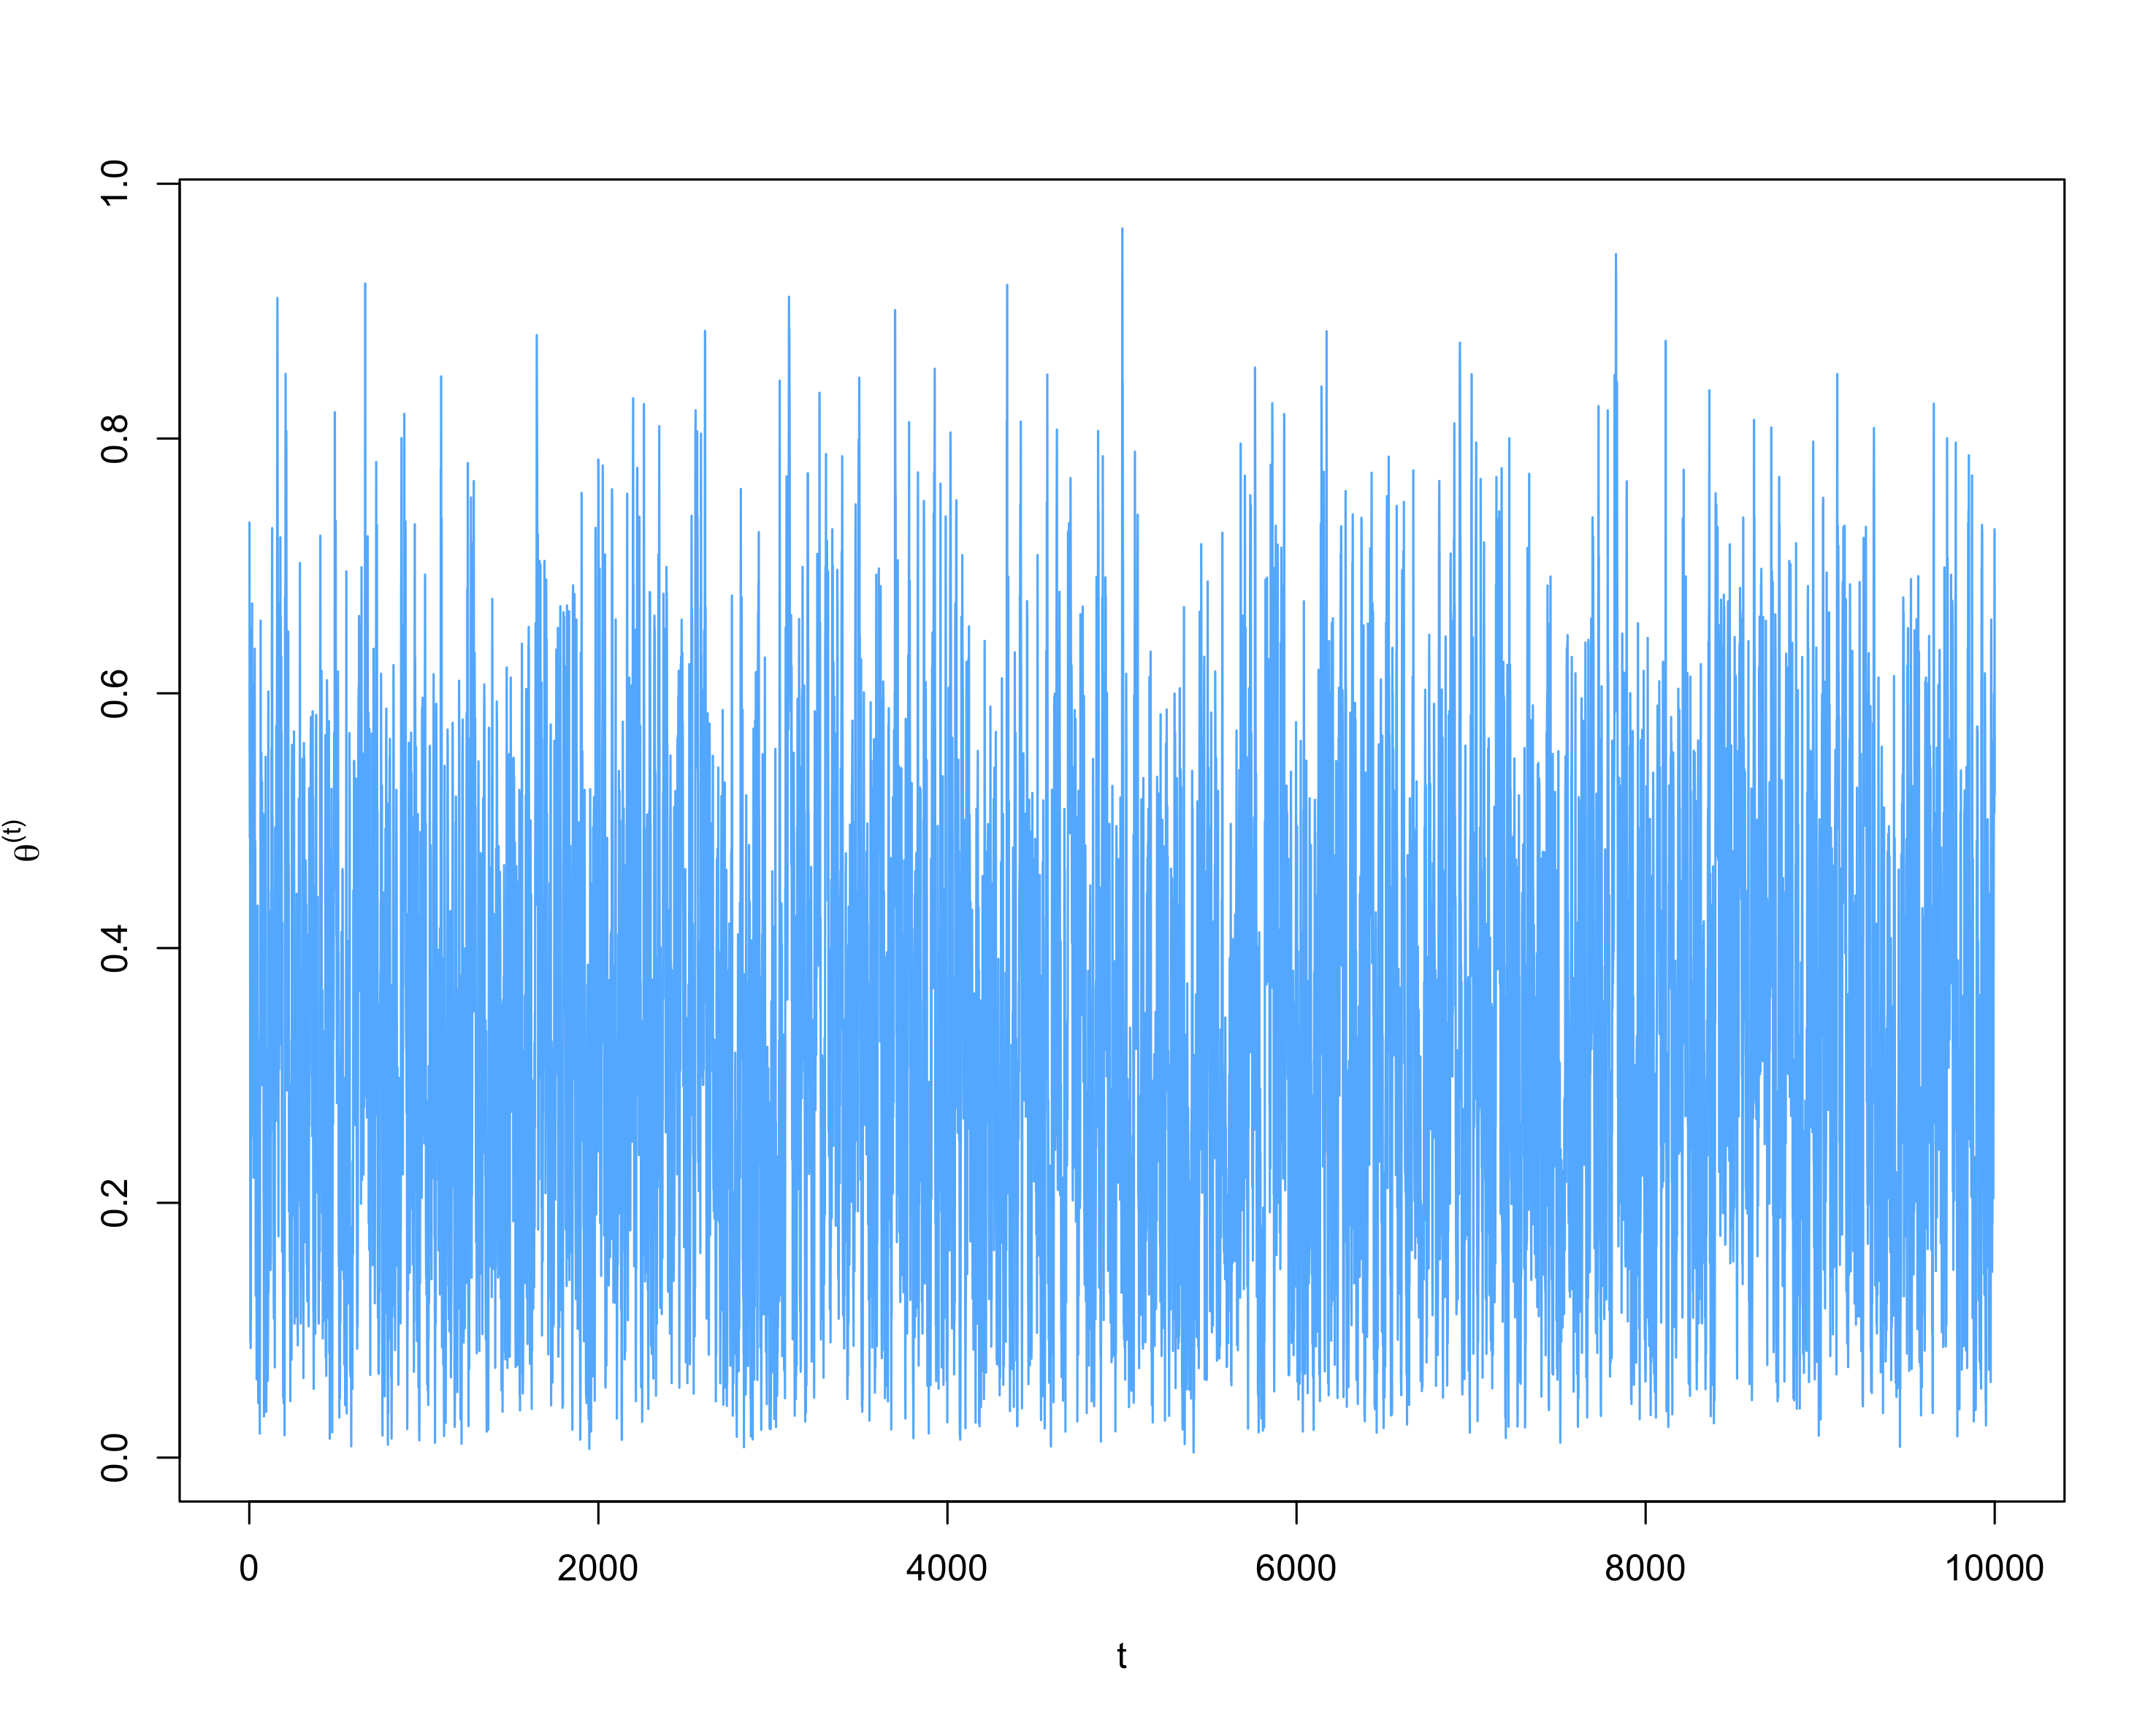
\includegraphics[width=\linewidth]{hier_chain_theta.png} 
        \caption{Proceso $\lbrace \theta_t \rbrace$} \label{fig:hier_chain_theta}
    \end{subfigure}
    
     \vspace{0.2cm}
    
    \begin{subfigure}[t]{0.45\textwidth}
        \centering
        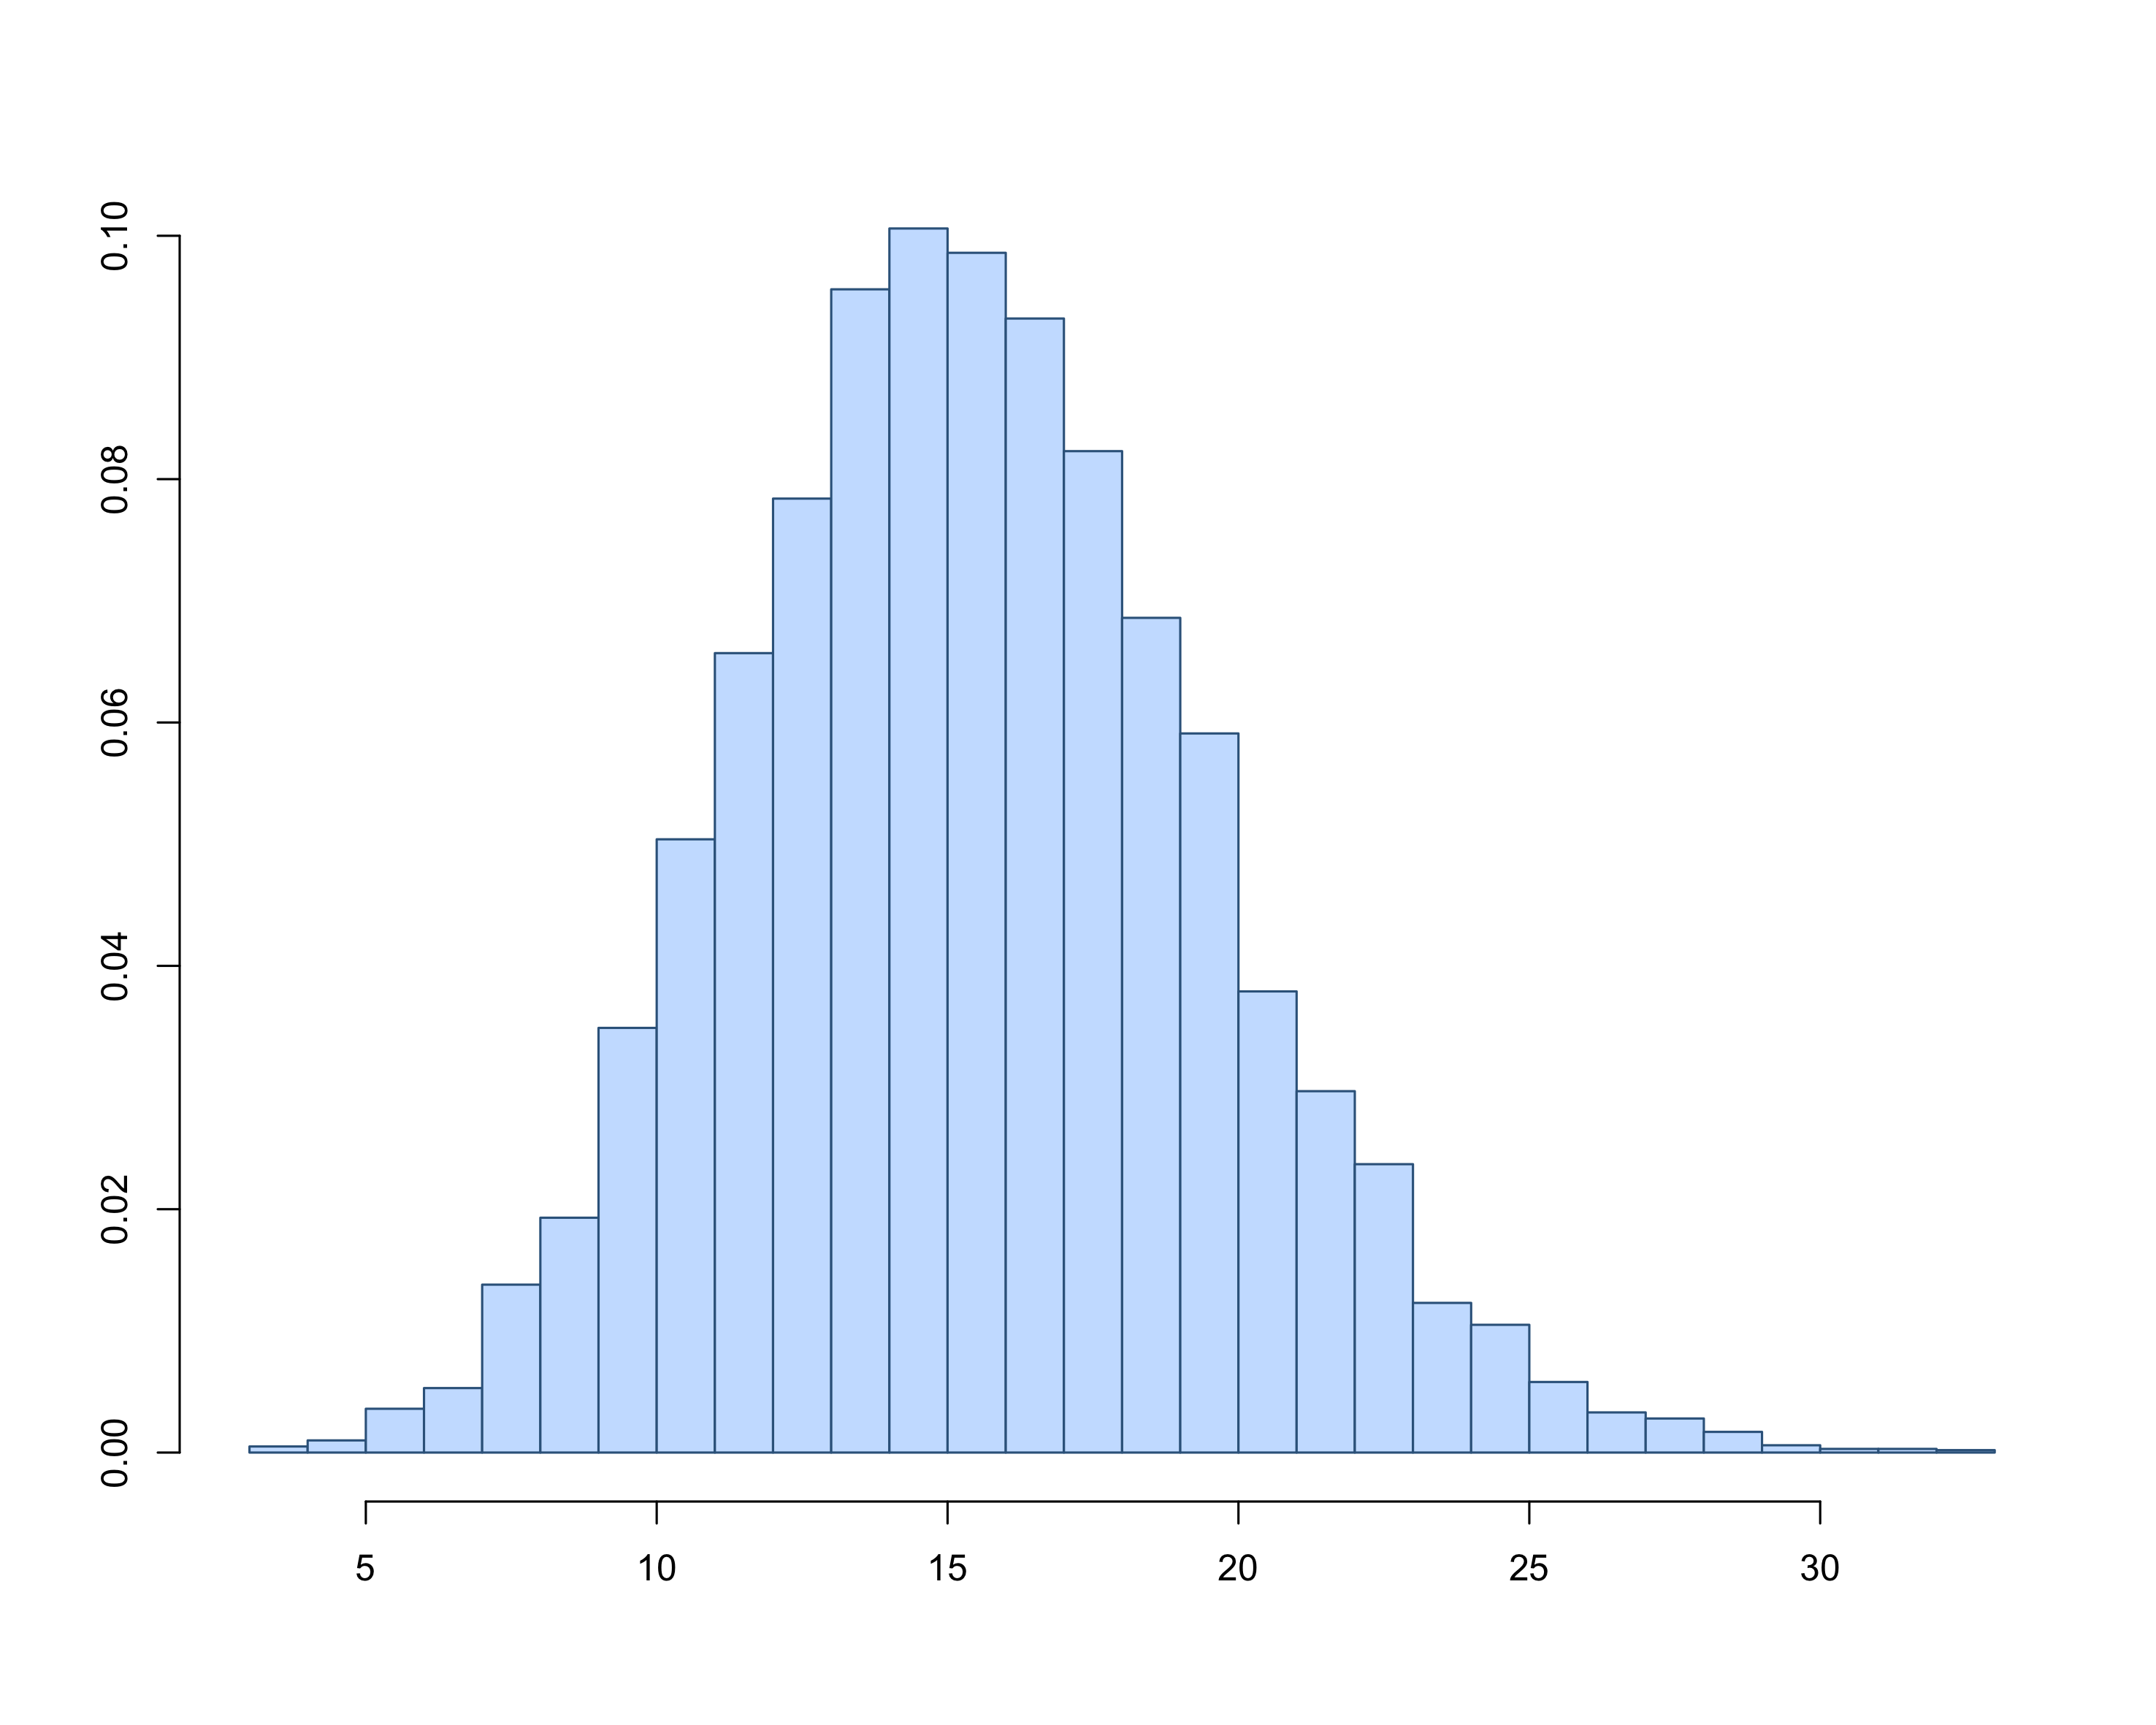
\includegraphics[width=\linewidth]{hier_hist_gamma.png} 
        \caption{Distribución marginal $f_\gamma$.} \label{fig:hier_hist_gamma}
    \end{subfigure}
    \hfill
    \begin{subfigure}[t]{0.45\textwidth}
        \centering
        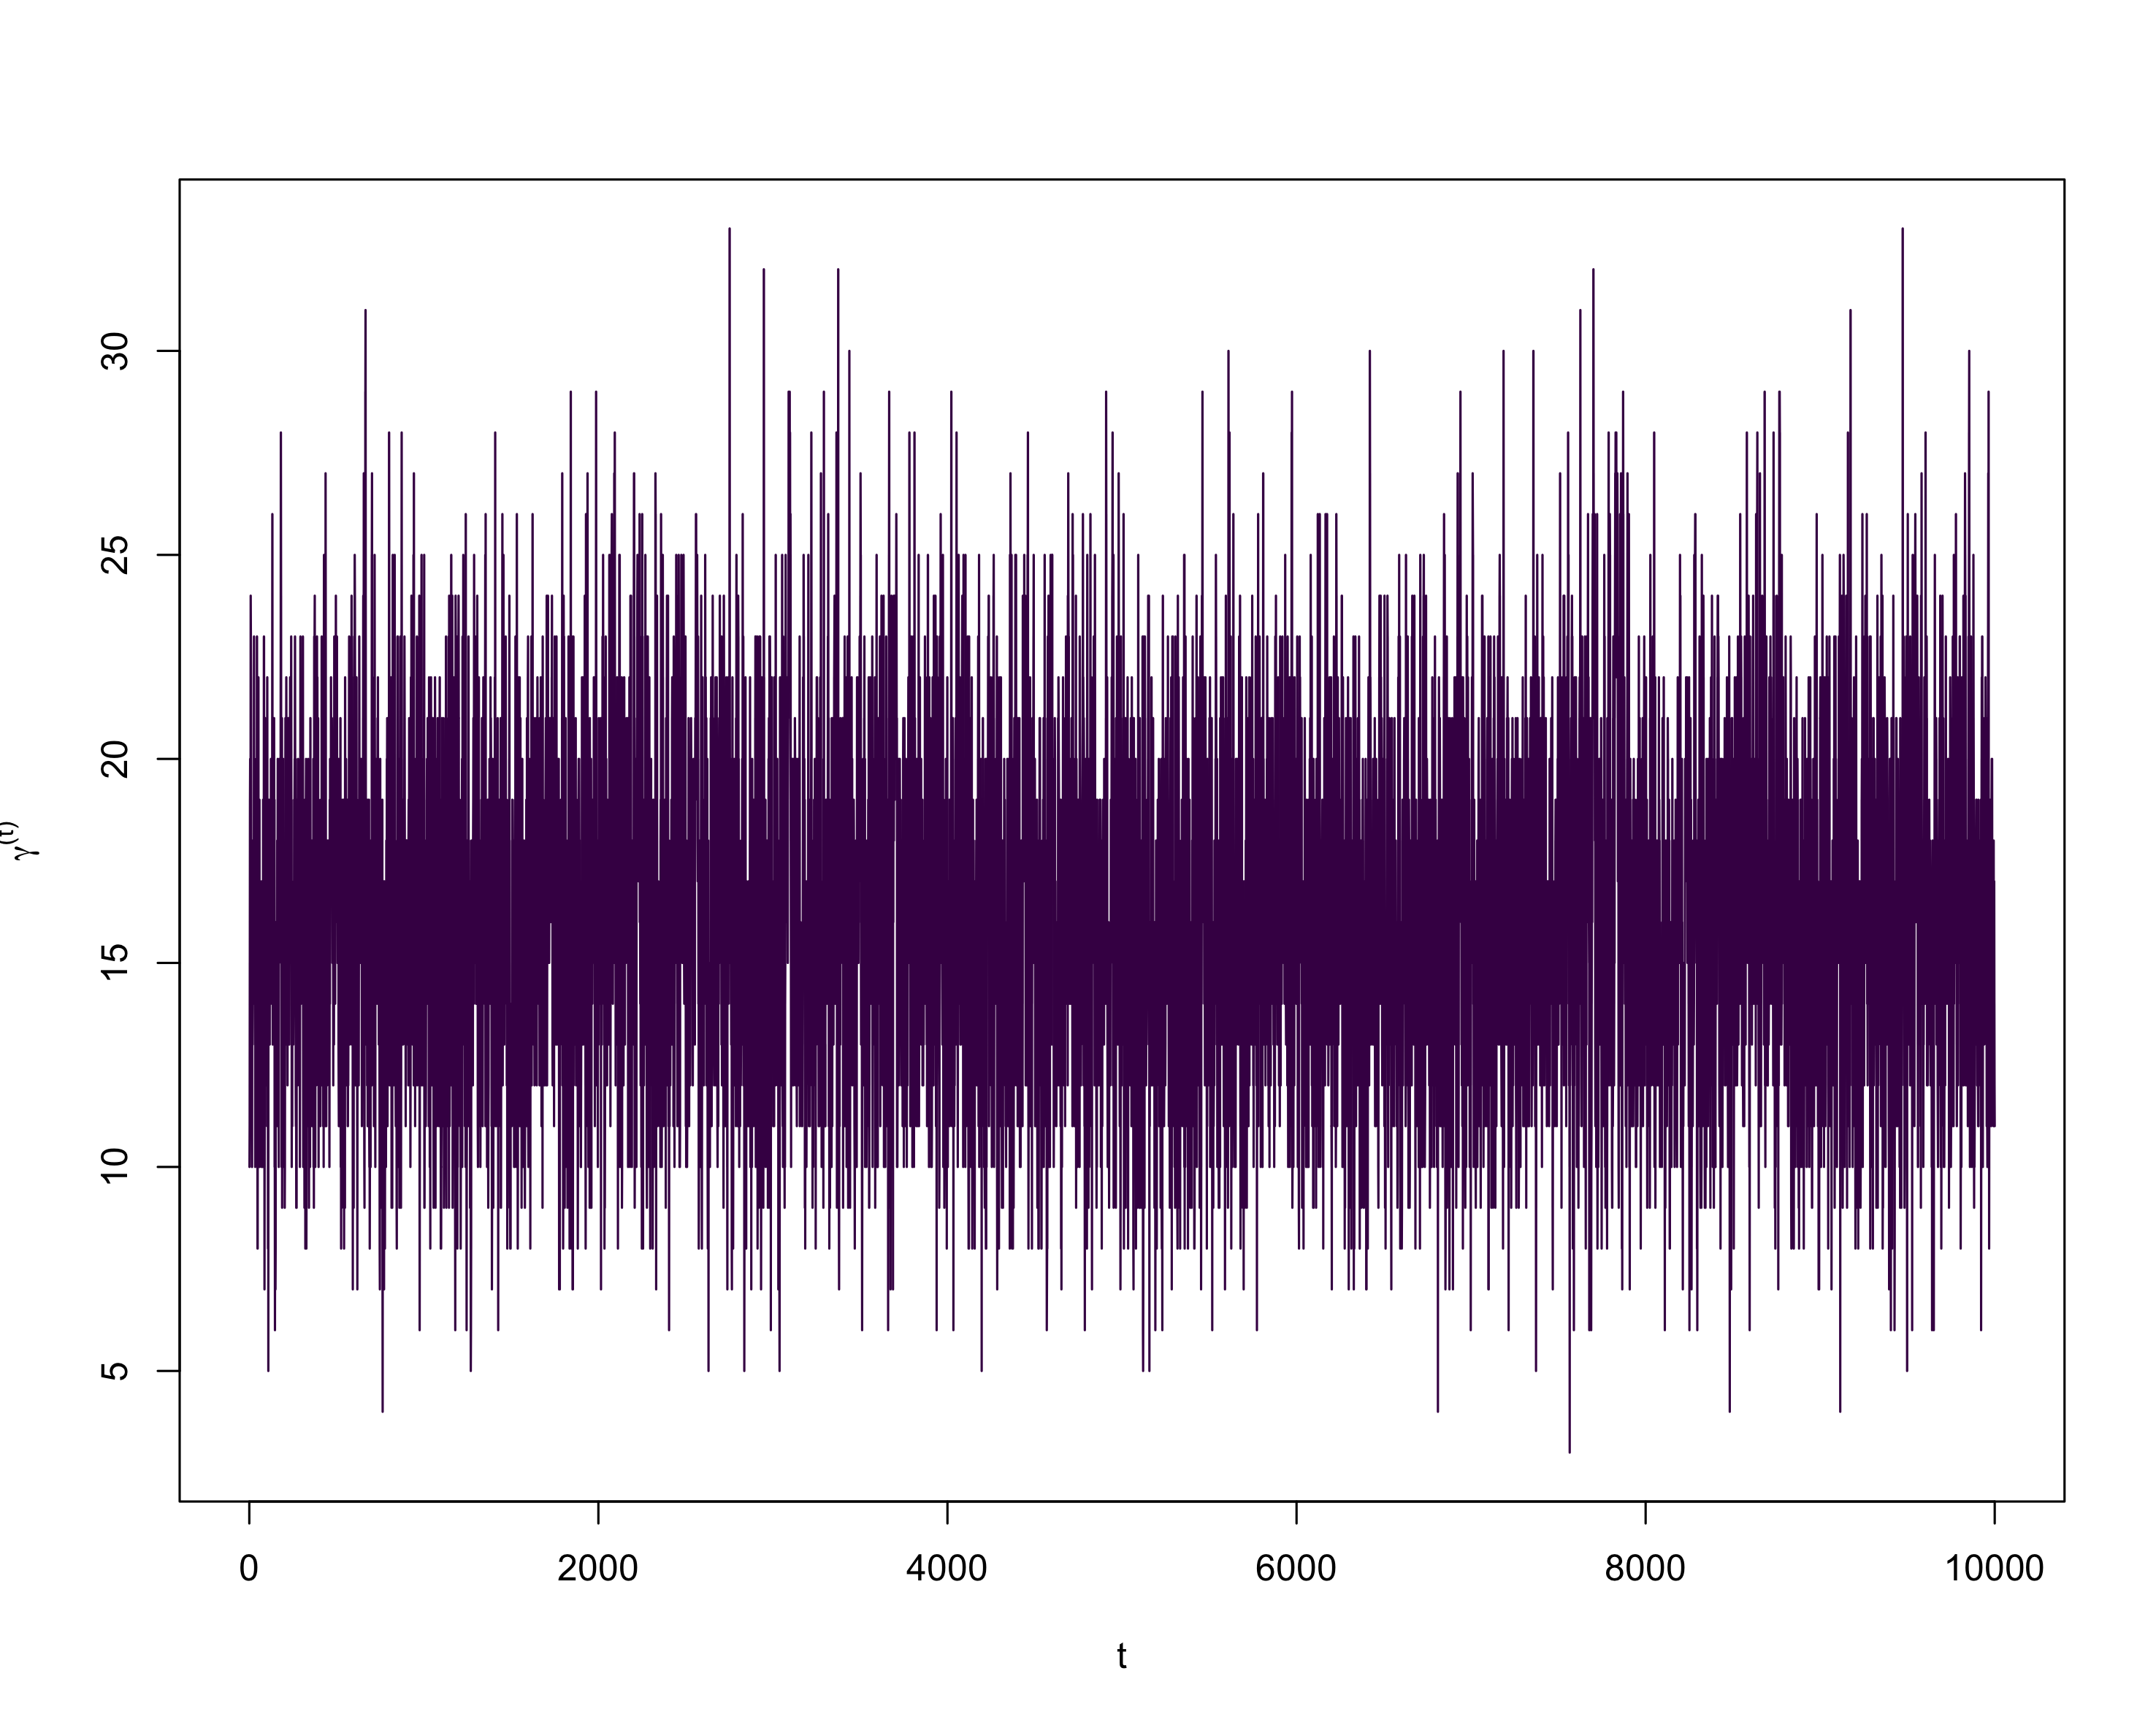
\includegraphics[width=\linewidth]{hier_chain_gamma.png} 
        \caption{Proceso $\lbrace \gamma_t \rbrace$} \label{fig:hier_chain_gamma}
    \end{subfigure}
    
    \caption{Simulaciones del modelo jerárquico utilizando el muestreador de Gibbs para tres variables con $\alpha = 2$, $\beta = 4$ y $\lambda = 16$.}
    \label{fig:gs_hier}
\end{figure}

En la figura \ref{fig:gs_hier} podemos ver los histogramas de cada una de las variables, junto con el estado que visitan los procesos en cada iteración. Como se verá más adelante, ver gráficamente los procesos es útil para analizar la convergencia del algoritmo.\\

Antes de pasar al algoritmo de Metropolis-Hastings, es muy importante resaltar que las observaciones obtenidas con el muestreador de Gibbs \textbf{no son una muestra aleatoria}, en el sentido de que las observaciones no son independientes. Esto siginifica que las hipótesis de la ley fuerte de los grandes números (teorema \ref{grandes_numeros}) no se cumplen para estas simulaciones. Sin embargo, existe un análogo a esta ley para cadenas de Markov ergódicas, conocido como el \textit{teorema ergódico} o \textit{de ergodicidad} \citep{casella}.

\begin{theorem}
Si un kernel de transición $P$ produce una cadena de Markov ergódica $\lbrace X_t \rbrace$ con distribución estacionaria $f$, entonces para una función integrable $h$ se cumple que
\begin{equation}
\lim_{T \to \infty} \sum_{t = 1}^T h(X^{(t)}) = E_f[h(X)].
\end{equation}
\end{theorem}


Este resultado es de suma importancia, ya que significa que podemos utilizar las observaciones simuladas con las cadenas de Markov para aproximar cantidades de interés con integración Monte Carlo. También resalta la importancia del análisis de convergencia para cadenas de Markov Monte Carlo, uno de los temas más estudiados para estos métodos. Hablaremos más del tema después de introducir el algoritmo de Metropolis-Hastings.\\

\subsection{Algoritmo de Metropolis-Hastings}
\label{sec:mh}

Antes de que Gelfand y Smith introdujeran el muestreador de Gibbs a la comunidad estadística, químicos y físicos ya estaban utilizando métodos de Monte Carlo en experimentos. En 1953, Nicholas Metropolis publicó un artículo en el que introdujo su algoritmo. Este artículo solamente trataba sobre el movimiento de partículas en un cuadrado y no mencionaba otras aplicaciones. En 1970, W. Keith Hastings generalizó el algoritmo de Metropolis. Sin embargo, la metodología siguió siendo ignorada en el ámbito estadístico debido a la poca disponibilidad de los recursos computacionales necesarios para explotarlo \citep{bertsch}.\\

Fue hasta después de la publicación de Gelfand y Smith que el muestreador de Gibbs fue identificado como un caso especial del algoritmo de Metropolis-Hastings. Hastings no supo de la gran importancia que tuvo su trabajo hasta después de su retiro en 1992, más de veinte años después de publicarlo \citep{bertsch}. Estudiemos ahora las principales características del algoritmo de Metropolis-Hastings.\\

La idea general del algoritmo de Metropolis-Hastings es parecida a los métodos de aceptación y rechazo de la sección \ref{aceptacion}, en el sentido de que se generan observaciones de una distribución candidata y con cierta probabilidad estas observaciones son aceptadas o no. Buscamos crear una cadena de Markov ergódica cuya distribución estacionaria sea la densidad de interés. Veamos cómo se construye esta cadena.\\

Si se tiene un kernel de transición $P$ que genera una cadena de Markov ergódica con distribución estacionaria $f$, entonces el kernel y la distribución satisfacen la condición \citep{chib_mh}
$$\int_{S_X} P(x, y)f(x) \ dx = f(y).$$ En nuestro caso conocemos la distribución estacionaria $f$ (nuestra distribución de interés). Lo que falta es encontrar el kernel de transición $P$. Para esto buscamos una función auxiliar $p(x, y)$ que satisfaga la condición de reversibilidad \citep{chib_mh}
\begin{equation} \label{eq:reversibilidad}
f(x)p(x, y) = f(y)p(y, x).
\end{equation}
Los mismos autores explican cómo encontrar esta función $p$.\\

Supongamos que tenemos una función de densidad que genera candidatos para la transición de la cadena. Denotemos a esta densidad $q(y|x)$, señalando que si el proceso se encuentra en el estado $x$, entonces la densidad genera un valor $y \sim q(y|x)$. Normalmente esta función no va a satisfacer la condición \eqref{eq:reversibilidad}, lo que significa que es más probable pasar al estado $y$ viniendo de $x$ que pasar al estado $x$ vieniendo de $y$ (o al revés). Entonces necesitamos ajustar la distribución candidata con una probabilidad $\alpha (x, y)$ de que el movimiento se realice. Entonces hasta ahora tenemos que, para $x \neq y$, $$p(x, y) = q(y | x) \alpha (x, y).$$\\

Suponiendo que $q$ no satisface la condición de reversibilidad porque la transición $x \to y$ es más probable que la transición $y \to x$, es decir, $$f(x)q(y|x) > f(y)q(x|y),$$ por lo que $$\frac{f(y)q(x|y)}{f(x)q(y|x)} < 1.$$ Entonces, queremos que la probabilidad $\alpha(y, x)$ sea lo más grande posible para compensar la baja probabilidad de la transición $y \to x$. Ya que fijamos $\alpha(y, x) = 1$, podemos obtener $\alpha(x, y)$ a partir de la ecuación \eqref{eq:reversibilidad}:\\

\begin{align*}
f(x)p(x, y) = f(y) p(y, x) &\implies f(x) q(y|x) \alpha(x, y) = f(y) q(x|y)\alpha (y, x)\\
&\implies f(x) q(y|x) \alpha(x, y) = f(y) q(x|y)\\
&\implies \alpha(x, y) = \frac{f(y)q(x|y)}{f(x)q(y|x)} < 1.\\
\end{align*}

En el caso contrario en que la condición de reversibilidad no se cumpla porque el paso $y \to x$ es más probable que el paso $x \to y$, entonces tendríamos que $$\frac{f(y)q(x|y)}{f(x)q(y|x)} > 1$$ y haríamos $\alpha(x, y) = 1$. Por lo tanto, si definimos
\begin{equation}
\label{eq:prob_transicion}
\alpha(x, y) = \min \lbrace \rho(x, y), 1 \rbrace,
\end{equation}
donde $\rho(x, y)$ es la razón de Hastings definida como $$\rho(x, y) = \frac{f(y)q(x|y)}{f(x)q(y|x)},$$ tenemos que $p(x, y)$ satisface la condición \eqref{eq:reversibilidad}. Por lo tanto, tenemos el kernel de transición buscado. Este kernel es de la siguiente forma. Si la cadena se encuentra en el estado $x^{(t)}$, generamos una observación candidata $y \sim q(y|x^{(t)})$ y hacemos
\begin{equation}
\label{eq:mh}
X^{(t+1)} = \begin{cases} 
      y & \text{con probabilidad } \alpha(x^{(t)}, y)\\
      x^{(t)} & \text{con probabilidad } 1-\alpha(x^{(t)}, y)
   \end{cases}.\\
\end{equation}

Es importante notar que, en teoría, este algoritmo funciona para cualquier distribución candidata $q$, siempre y cuando esta densidad explore todo el soporte de la densidad de interés. Esto significa que no necesitamos satisfacer la condición del método de aceptación y rechazo de encontrar una cota $M$ para el cociente de las densidades. Sin embargo, en la práctica la selección de $q$ va a impactar de manera importante la efectividad de las simulaciones. Veamos ahora algunas maneras de elegir esta distribución candidata.\\

Una manera de elegir la distribución candidata es hacerla independiente del valor de la cadena $x^{(t)}$, es decir, $q(y|x) = g(y)$. De esta manera, la razón de Hastings se simplifica a $$\rho (x, y) = \frac{f(y)g(x)}{f(x)g(y)}.$$ Sin embargo, \citet{casella} señalan que este tipo de propuestas son imprácticas debido a la dificultad de crear propuestas adecuadas en algunos contextos. Los mismos autores sugieren explorar vecindades del valor de la cadena en la iteración anterior para ir descubriendo paso a paso las propiedades de la distribución objetivo.\\

Una manera de explorar estas vecindades es utilizando caminatas aleatorias de la forma $y = x^{(t)} + \epsilon$. Si la distribución de $\epsilon$ es simétrica, esto es que $f_{\epsilon} = f_{-\epsilon}$, entonces se cumple que $q(y|x) = q(x|y)$ y la razón de Hastings es simplemente $$\rho (x, y) = \frac{f(y)}{f(x)}.$$ El caso de estas propuestas simétricas fue el estudiado originalmente por Metropolis en 1953 \citep{gelman}. A veces se utiliza el nombre de algoritmo de Metropolis para indicar este tipo de distribuciones candidatas. Note el lector que si la caminata aleatoria no es simétrica, entonces se debe incorporar el cociente de la densidad candidata a la razón de Hastings.\\

Ya que revisamos las propiedades del algoritmo de Metropolis-Hastings, entendamos por qué el muestreador de Gibbs es un caso especial de éste. Digamos que la iteración $t$ del algoritmo de Metropolis-Hastings es una serie de $p$ pasos, donde cada uno corresponde a un subvector $\theta_i$ de $\theta$. El $i$-ésimo paso de la iteración $t$ solamente mueve el subvector $\theta_i$ utilizando la densidad condicional de $\theta_i | \theta^{(t-1)}_{-i}$ \citep{gelman}:
$$q_i(\theta^* | \theta^{(t-1)}) = \begin{cases}
f_{\theta_i | \theta_{-i}^{(t-1)}} (\theta^*_{i}) & \text{si } \theta^*_{-i} = \theta^{(t-1)}_{-i}\\
0 & \text{en otro caso} \end{cases}.$$

De esta forma, la razón de Hastings es
\begin{align*}
\rho(\theta^{(t-1)}, \theta^*) &= \frac{f(\theta^*) \ q_i(\theta^{(t-1)}|\theta^*)}{f(\theta^{(t-1)}) \ q_i(\theta^*|\theta^{(t-1)})}\\
&= \frac{f(\theta^*) \ f_{\theta_i|\theta_{-i}^{(t-1)}}(\theta^{(t-1)})}{f(\theta^{(t-1)}) \ f_{\theta_i|\theta_{-i}^{(t-1)}}(\theta^*)}\\
&= \frac{f(\theta^*)f(\theta^{(t-1)})}{f(\theta^{(t-1)})f(\theta^*)}\\
&= 1,
\end{align*}
donde $$\frac{f_{\theta_i|\theta_{-i}^{(t-1)}}(\theta^{(t-1)})}{f_{\theta_i|\theta_{-i}^{(t-1)}}(\theta^*)} = \frac{f(\theta^{(t-1)})}{f(\theta^*)}$$ porque $\theta_{-i}^* = \theta_{-i}^{(t-1)}$.\\

Esto prueba que el muestreador de Gibbs es un caso especial del algoritmo de Metropolis-Hastings. También es interesante resaltar que el hecho de que  $\rho(\theta^{(t-1)}, \theta^*) = 1$ en el caso anterior, explica por qué la observación propuesta siempre es aceptada en el muestreador de Gibbs.\\

Veamos ahora un ejemplo de cómo utilizar el algoritmo de Metropolis-Hastings. La distribución objetivo es una $t_{(5)}$ y compararemos tres distribuciones candidatas diferentes:
\begin{enumerate}
\item $q_1$ independiente, $q_1(y|x) = g(y) \sim \mathcal{N}(0, 1).$
\item Caminata aleatoria simétrica $q_2(y|x) \sim \mathcal{N}(x, 1).$
\item Caminata aleatoria simétrica $q_3(y|x) \sim U(x - 1, x + 1).$
\end{enumerate}
Llamamos $\lbrace X_t^i \rbrace$ a la cadena generada con la distribución candidata $q_i$.\\

\begin{figure}
    \centering
    \begin{subfigure}[t]{0.45\textwidth}
        \centering
        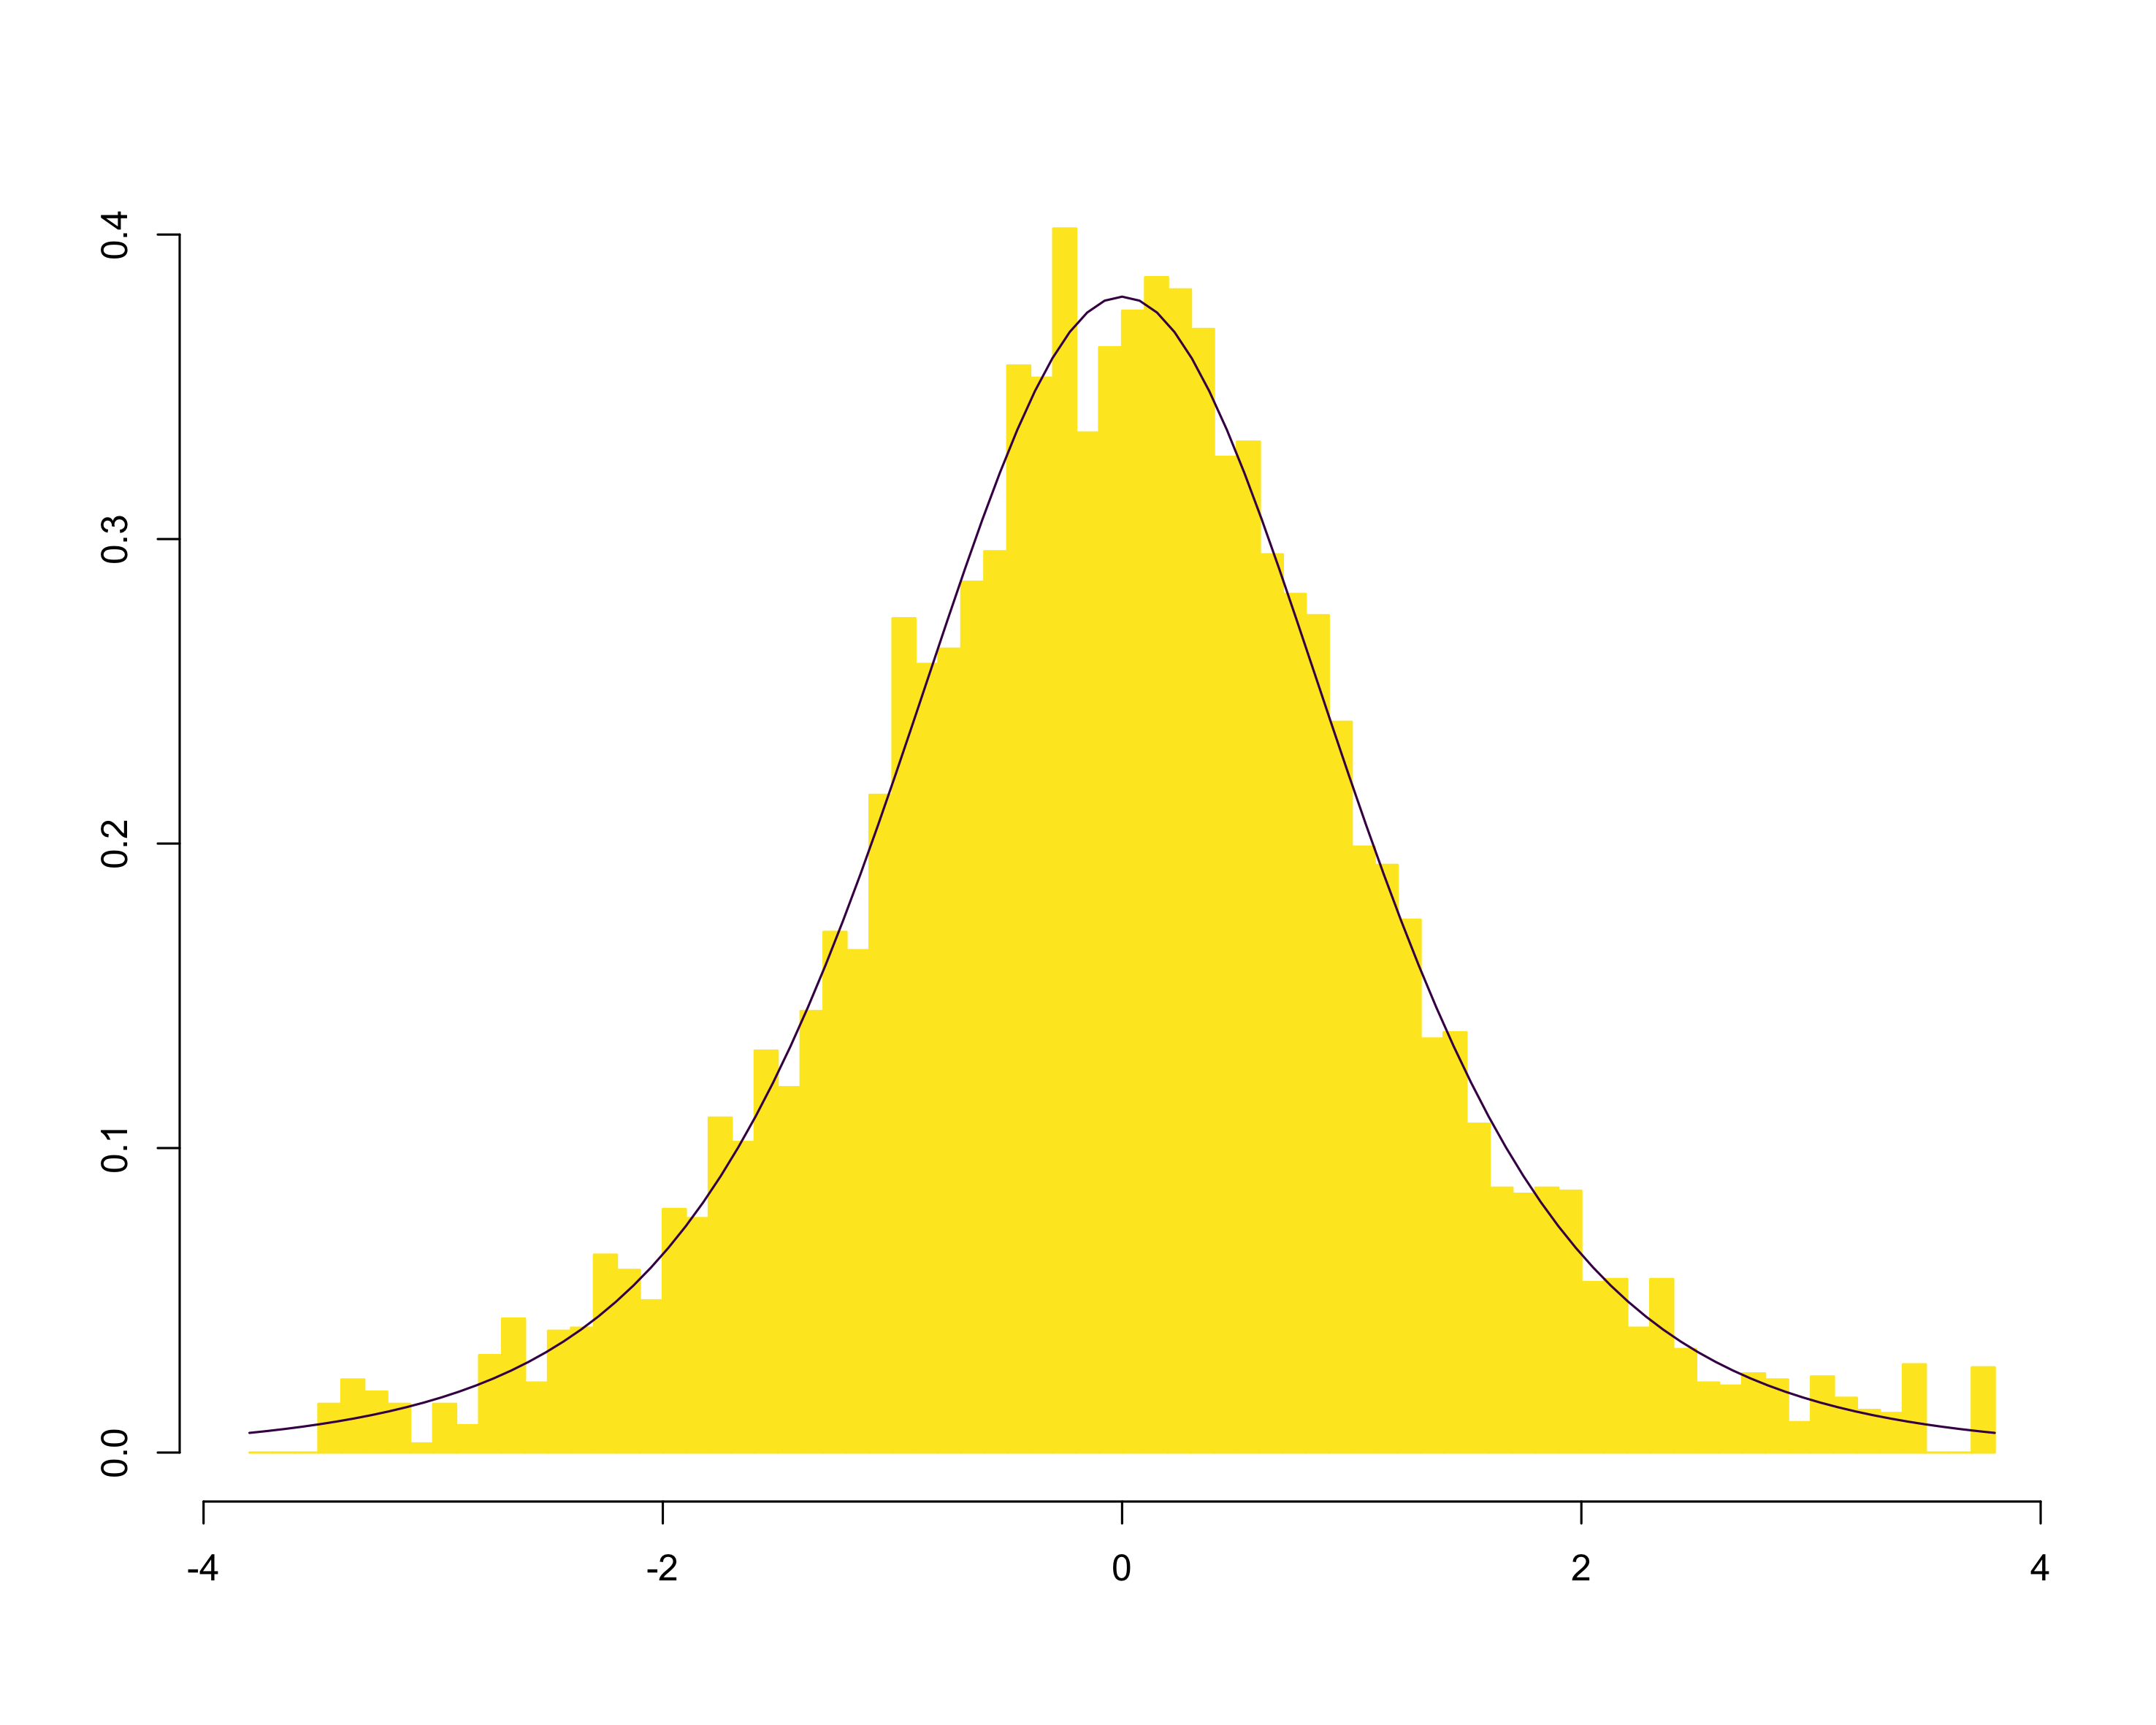
\includegraphics[width=\linewidth]{mh_hist_x1.png} 
        \caption{Histograma de $f \sim t_{(5)}$ con propuestas $q_1$} \label{fig:mh_hist_x1}
    \end{subfigure}
    \hfill
    \begin{subfigure}[t]{0.45\textwidth}
        \centering
        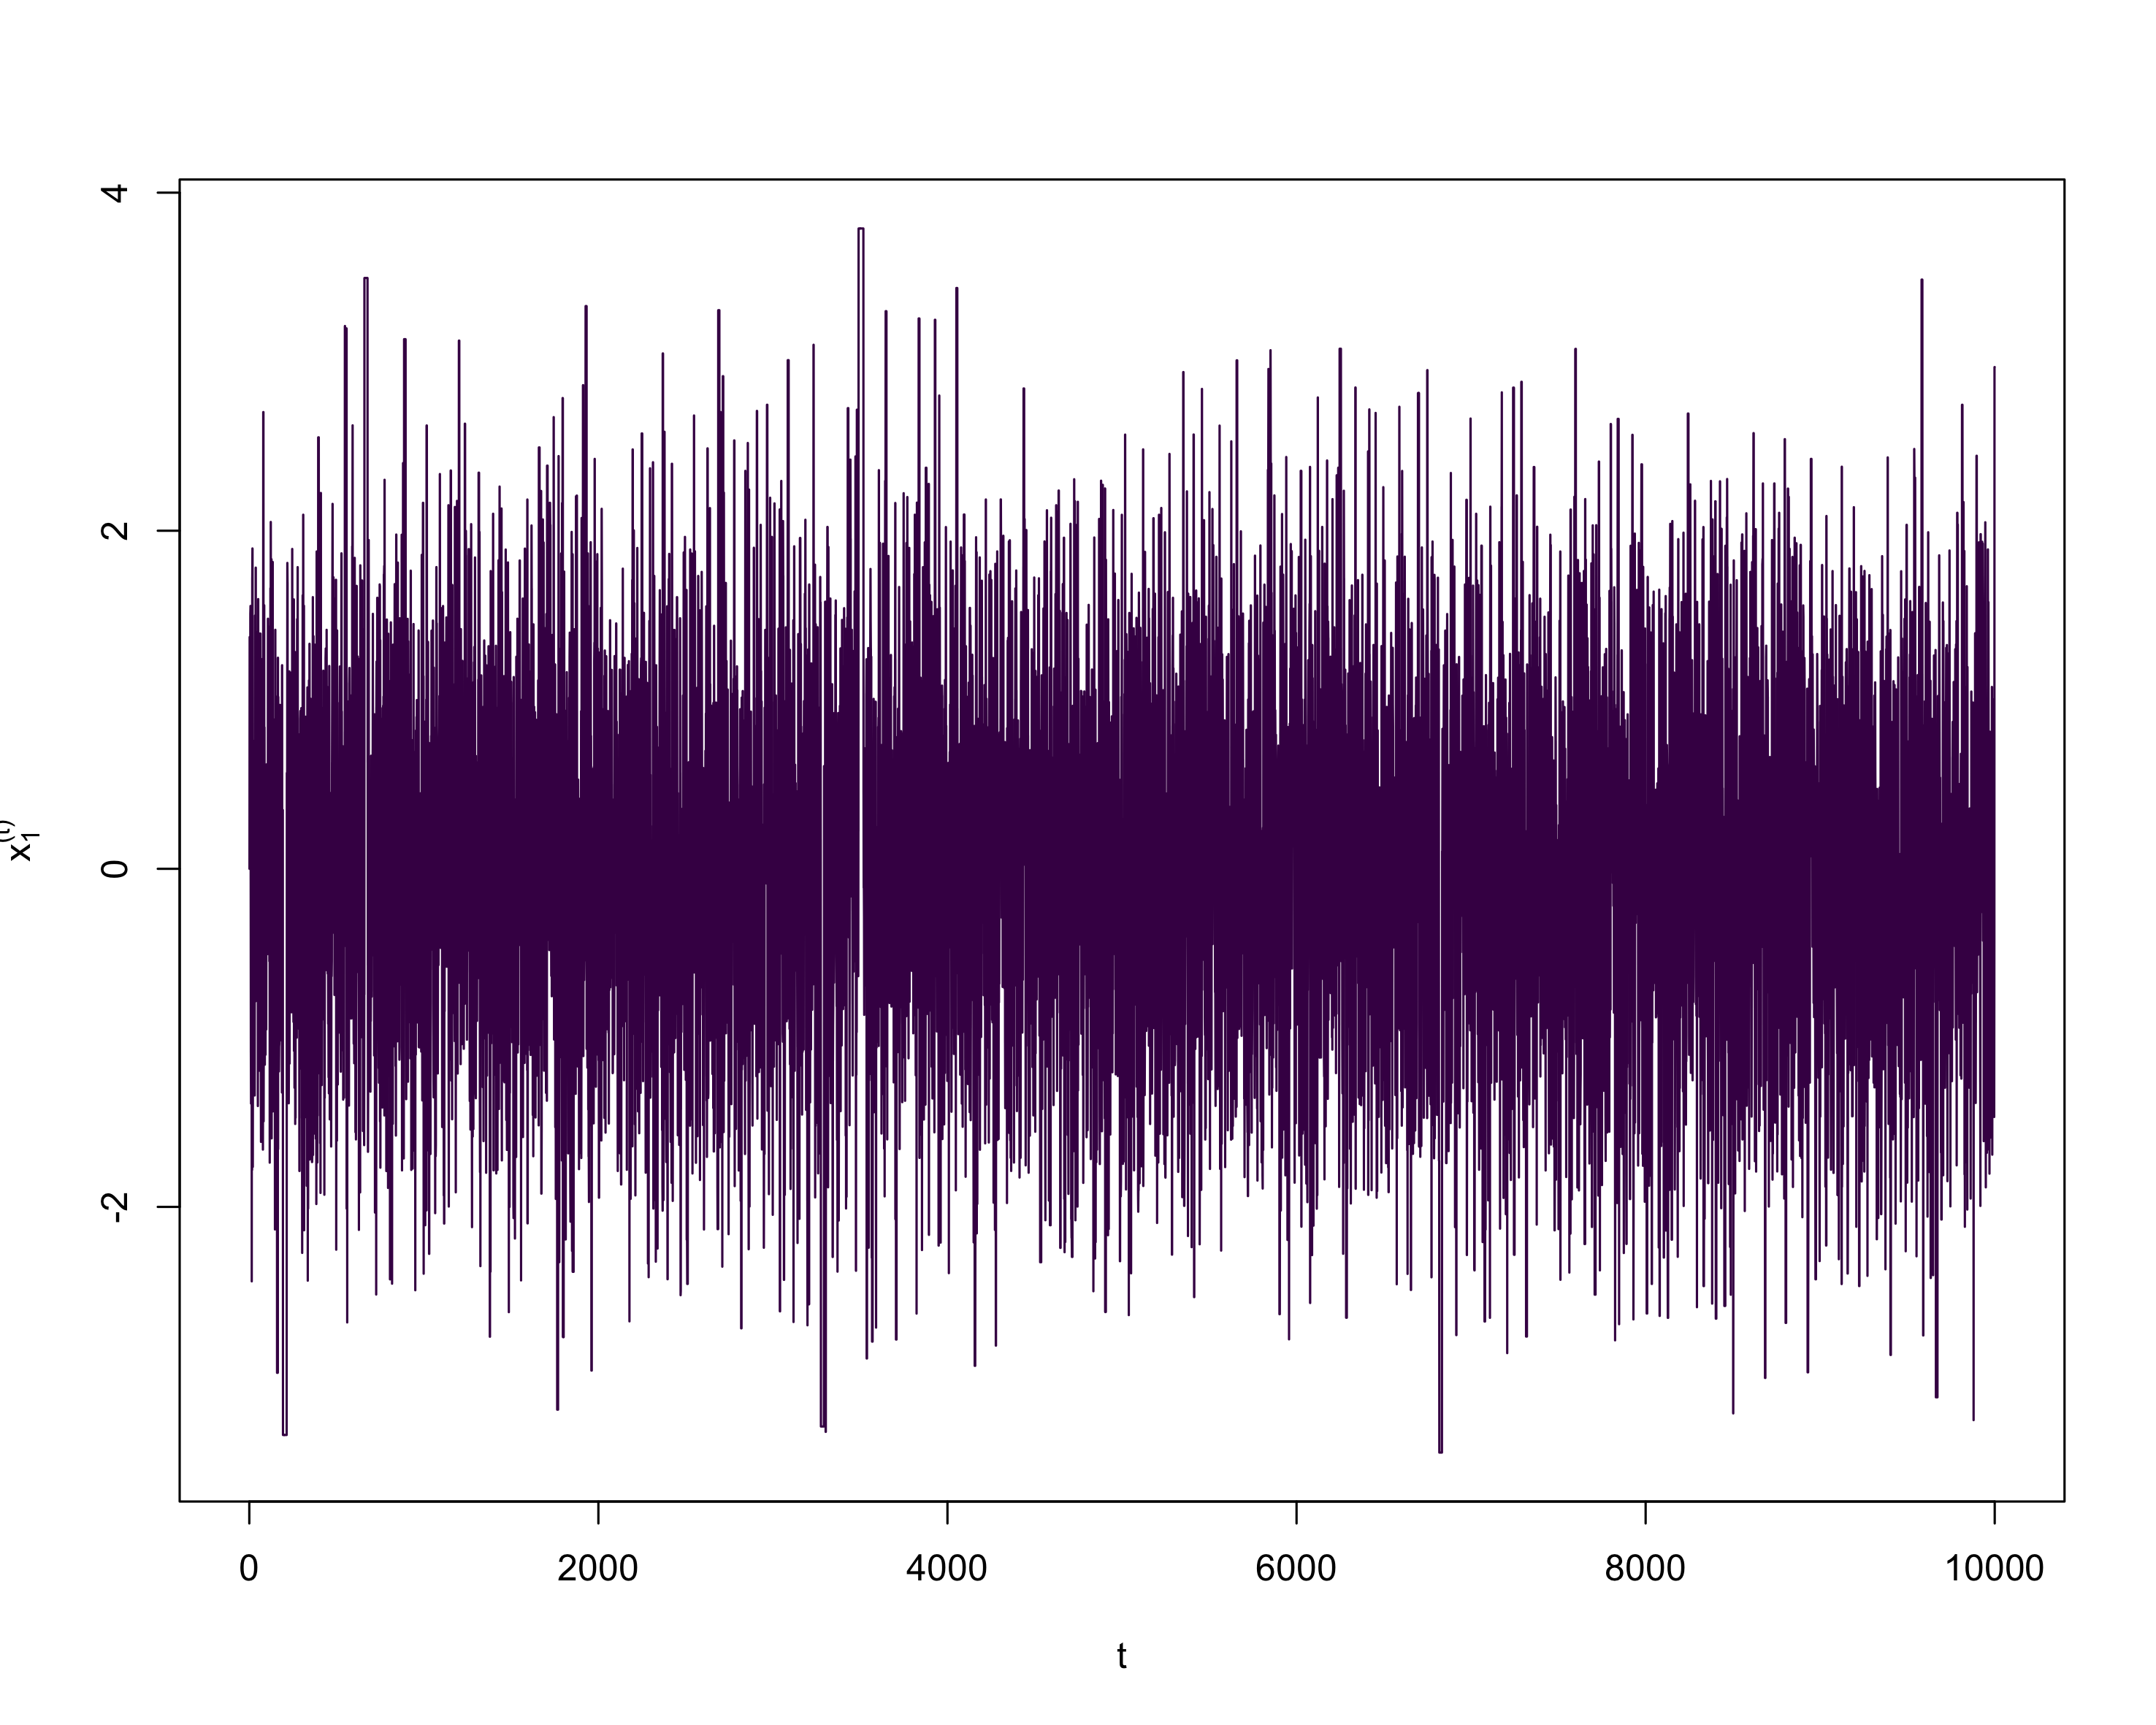
\includegraphics[width=\linewidth]{mh_chain_x1.png} 
        \caption{Proceso $\lbrace X_t^1 \rbrace$} \label{fig:mh_chain_x1}
    \end{subfigure}

    \vspace{0.2cm}
    
    \begin{subfigure}[t]{0.45\textwidth}
        \centering
        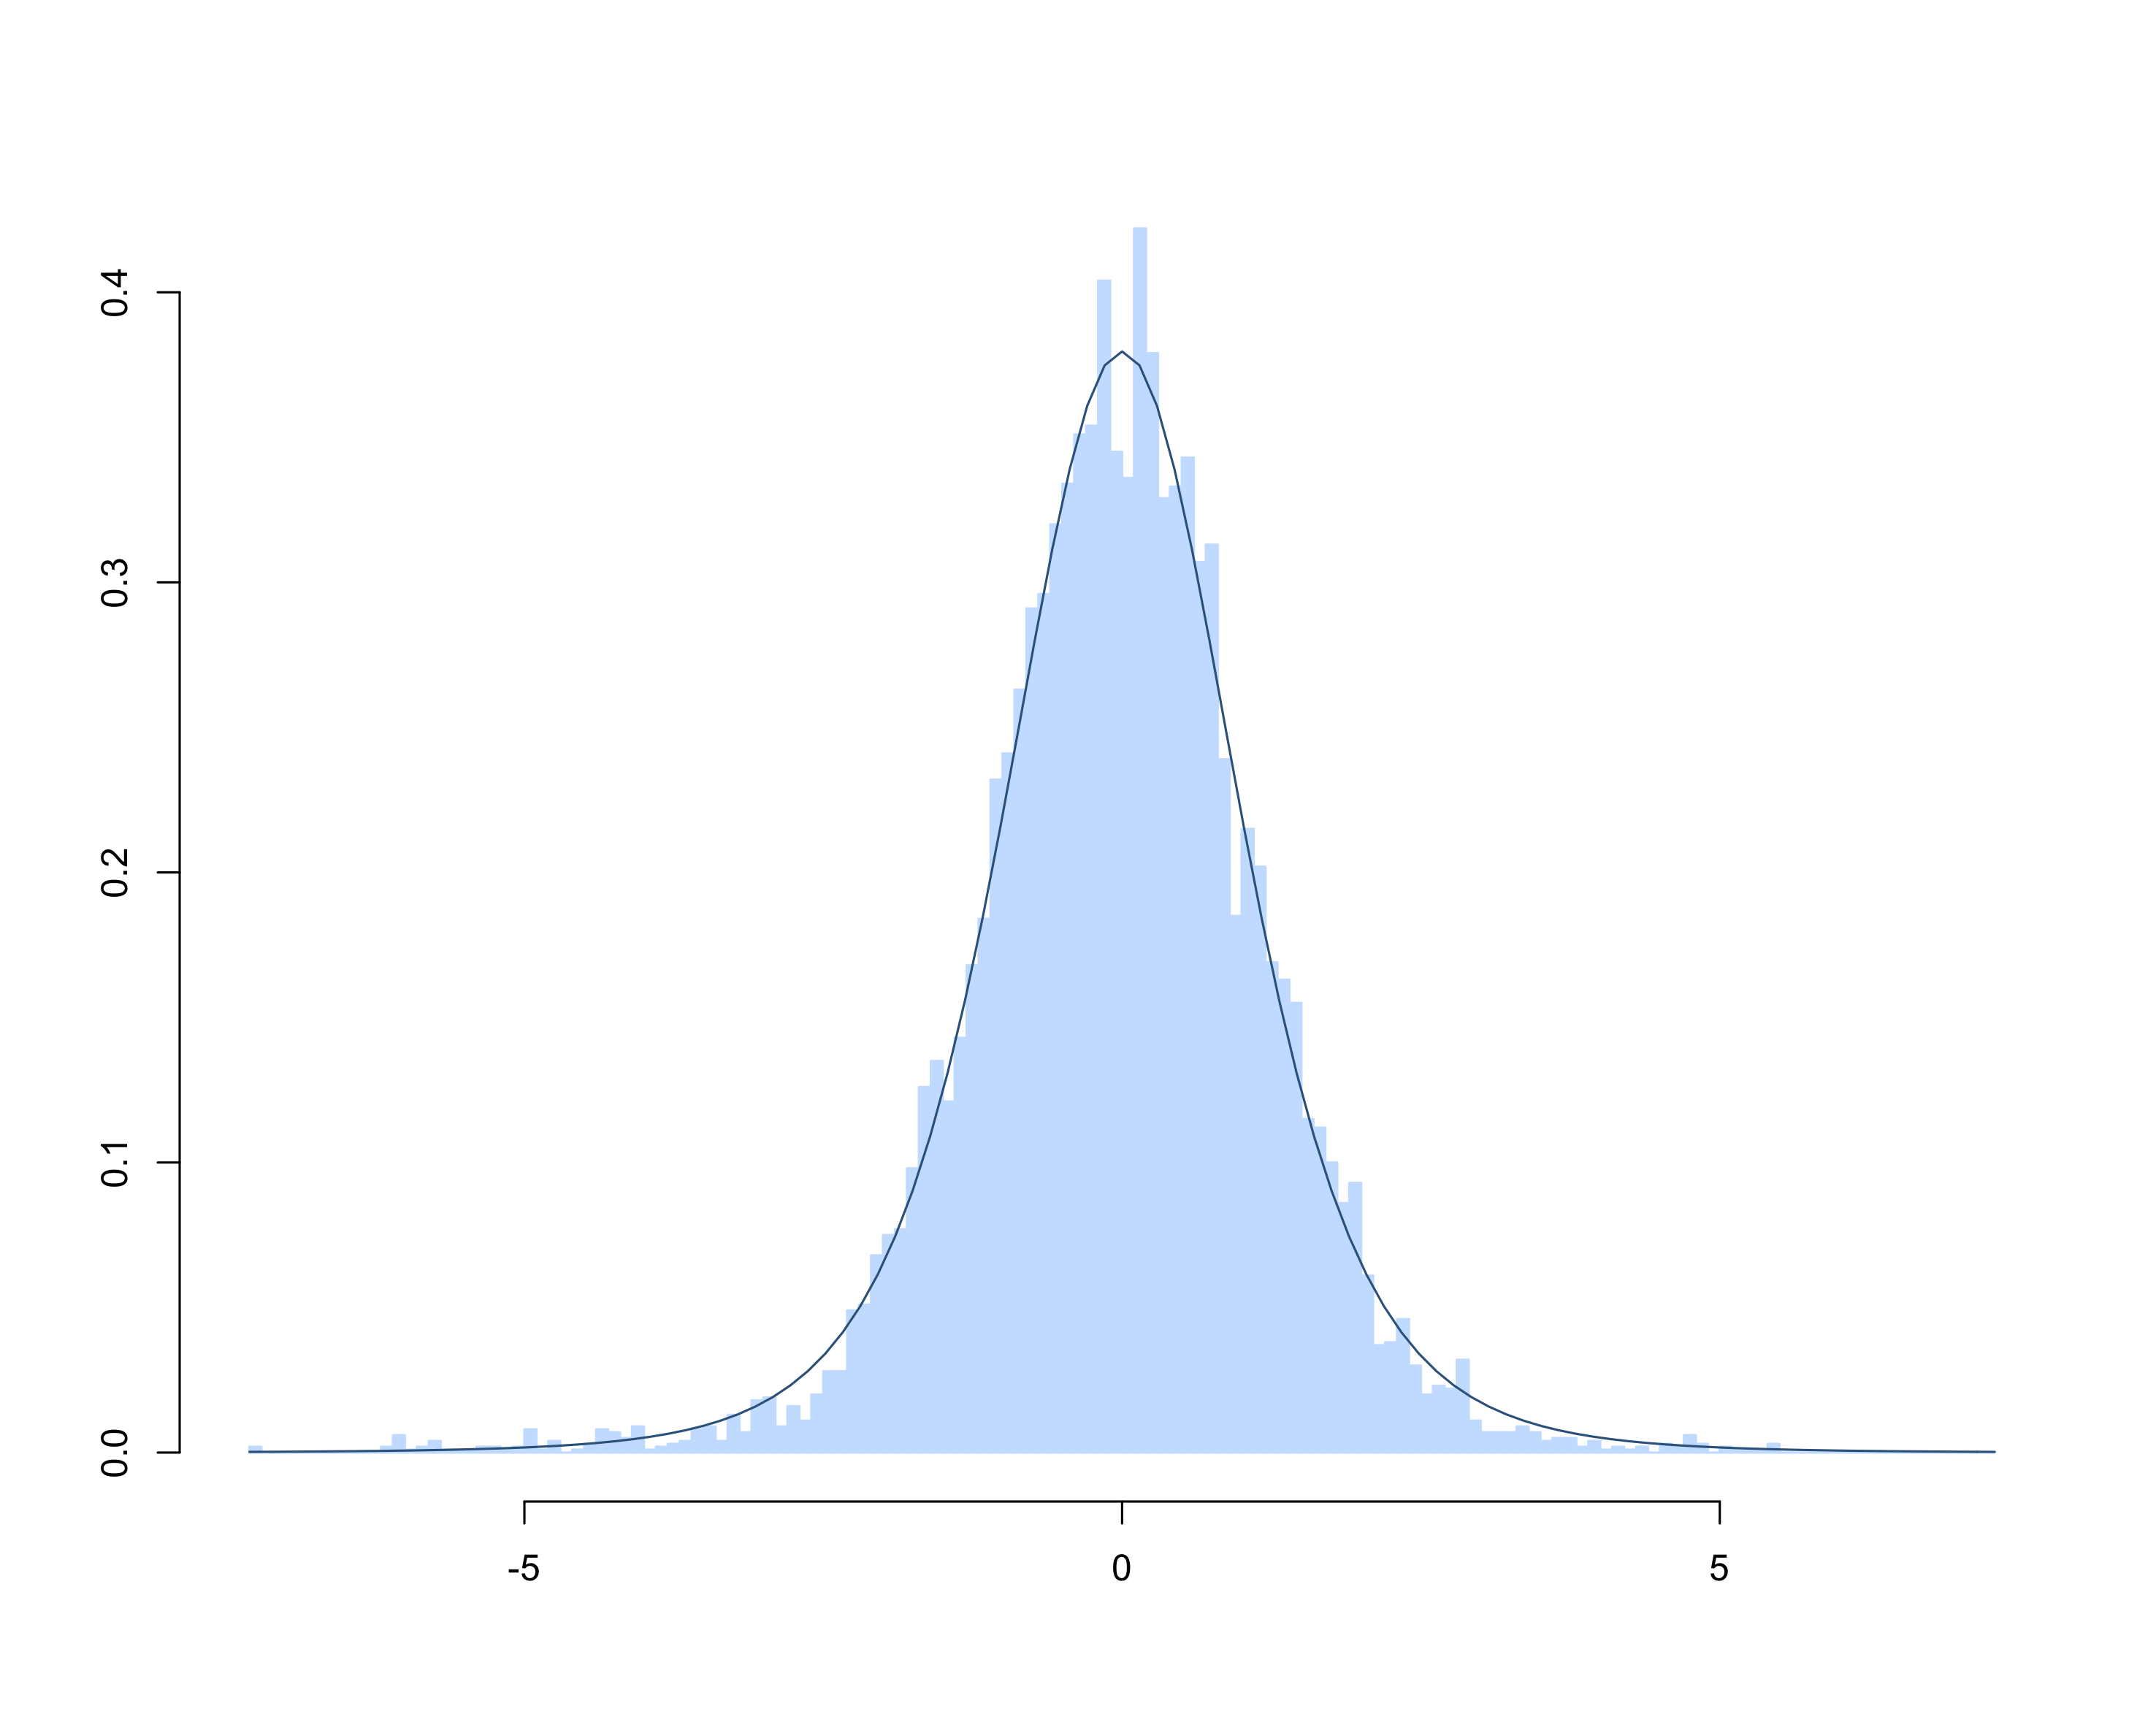
\includegraphics[width=\linewidth]{mh_hist_x2.png} 
        \caption{Histograma de $f \sim t_{(5)}$ con propuestas $q_2$} \label{fig:mh_hist_x2}
    \end{subfigure}
    \hfill
    \begin{subfigure}[t]{0.45\textwidth}
        \centering
        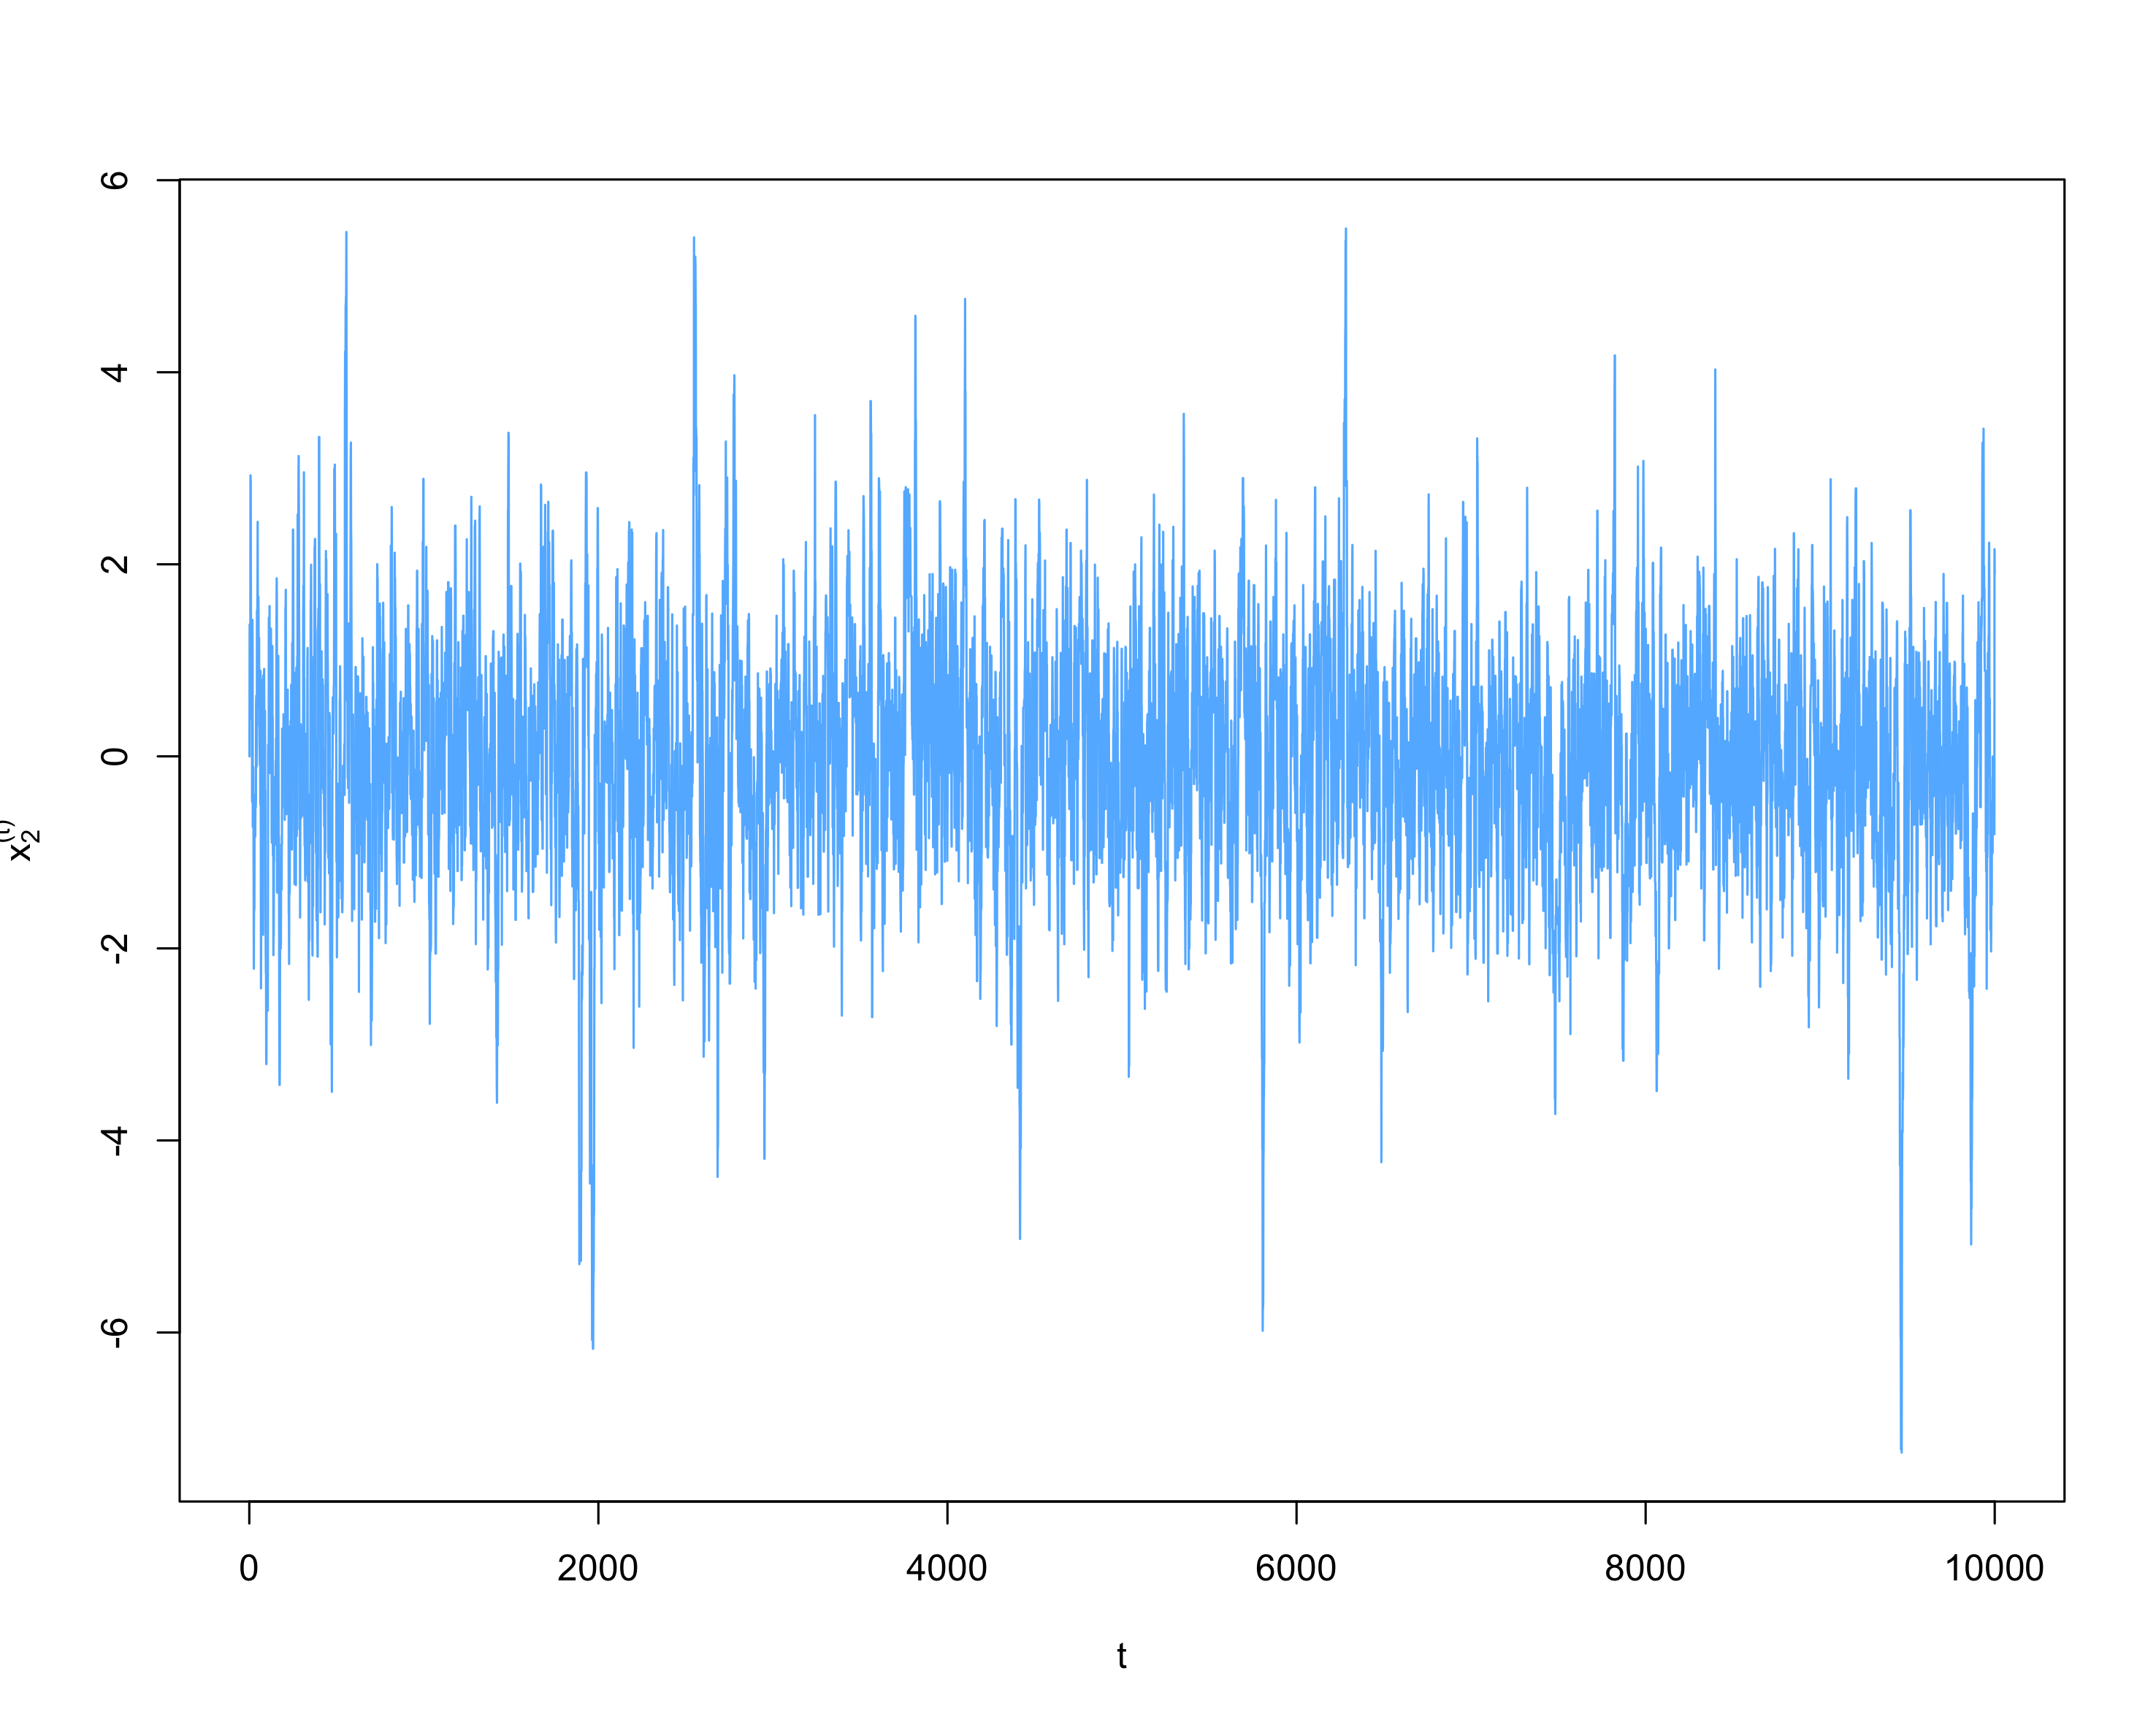
\includegraphics[width=\linewidth]{mh_chain_x2.png} 
        \caption{Proceso $\lbrace X_t^2 \rbrace$} \label{fig:mh_chain_x2}
    \end{subfigure}
    
     \vspace{0.2cm}
    
    \begin{subfigure}[t]{0.45\textwidth}
        \centering
        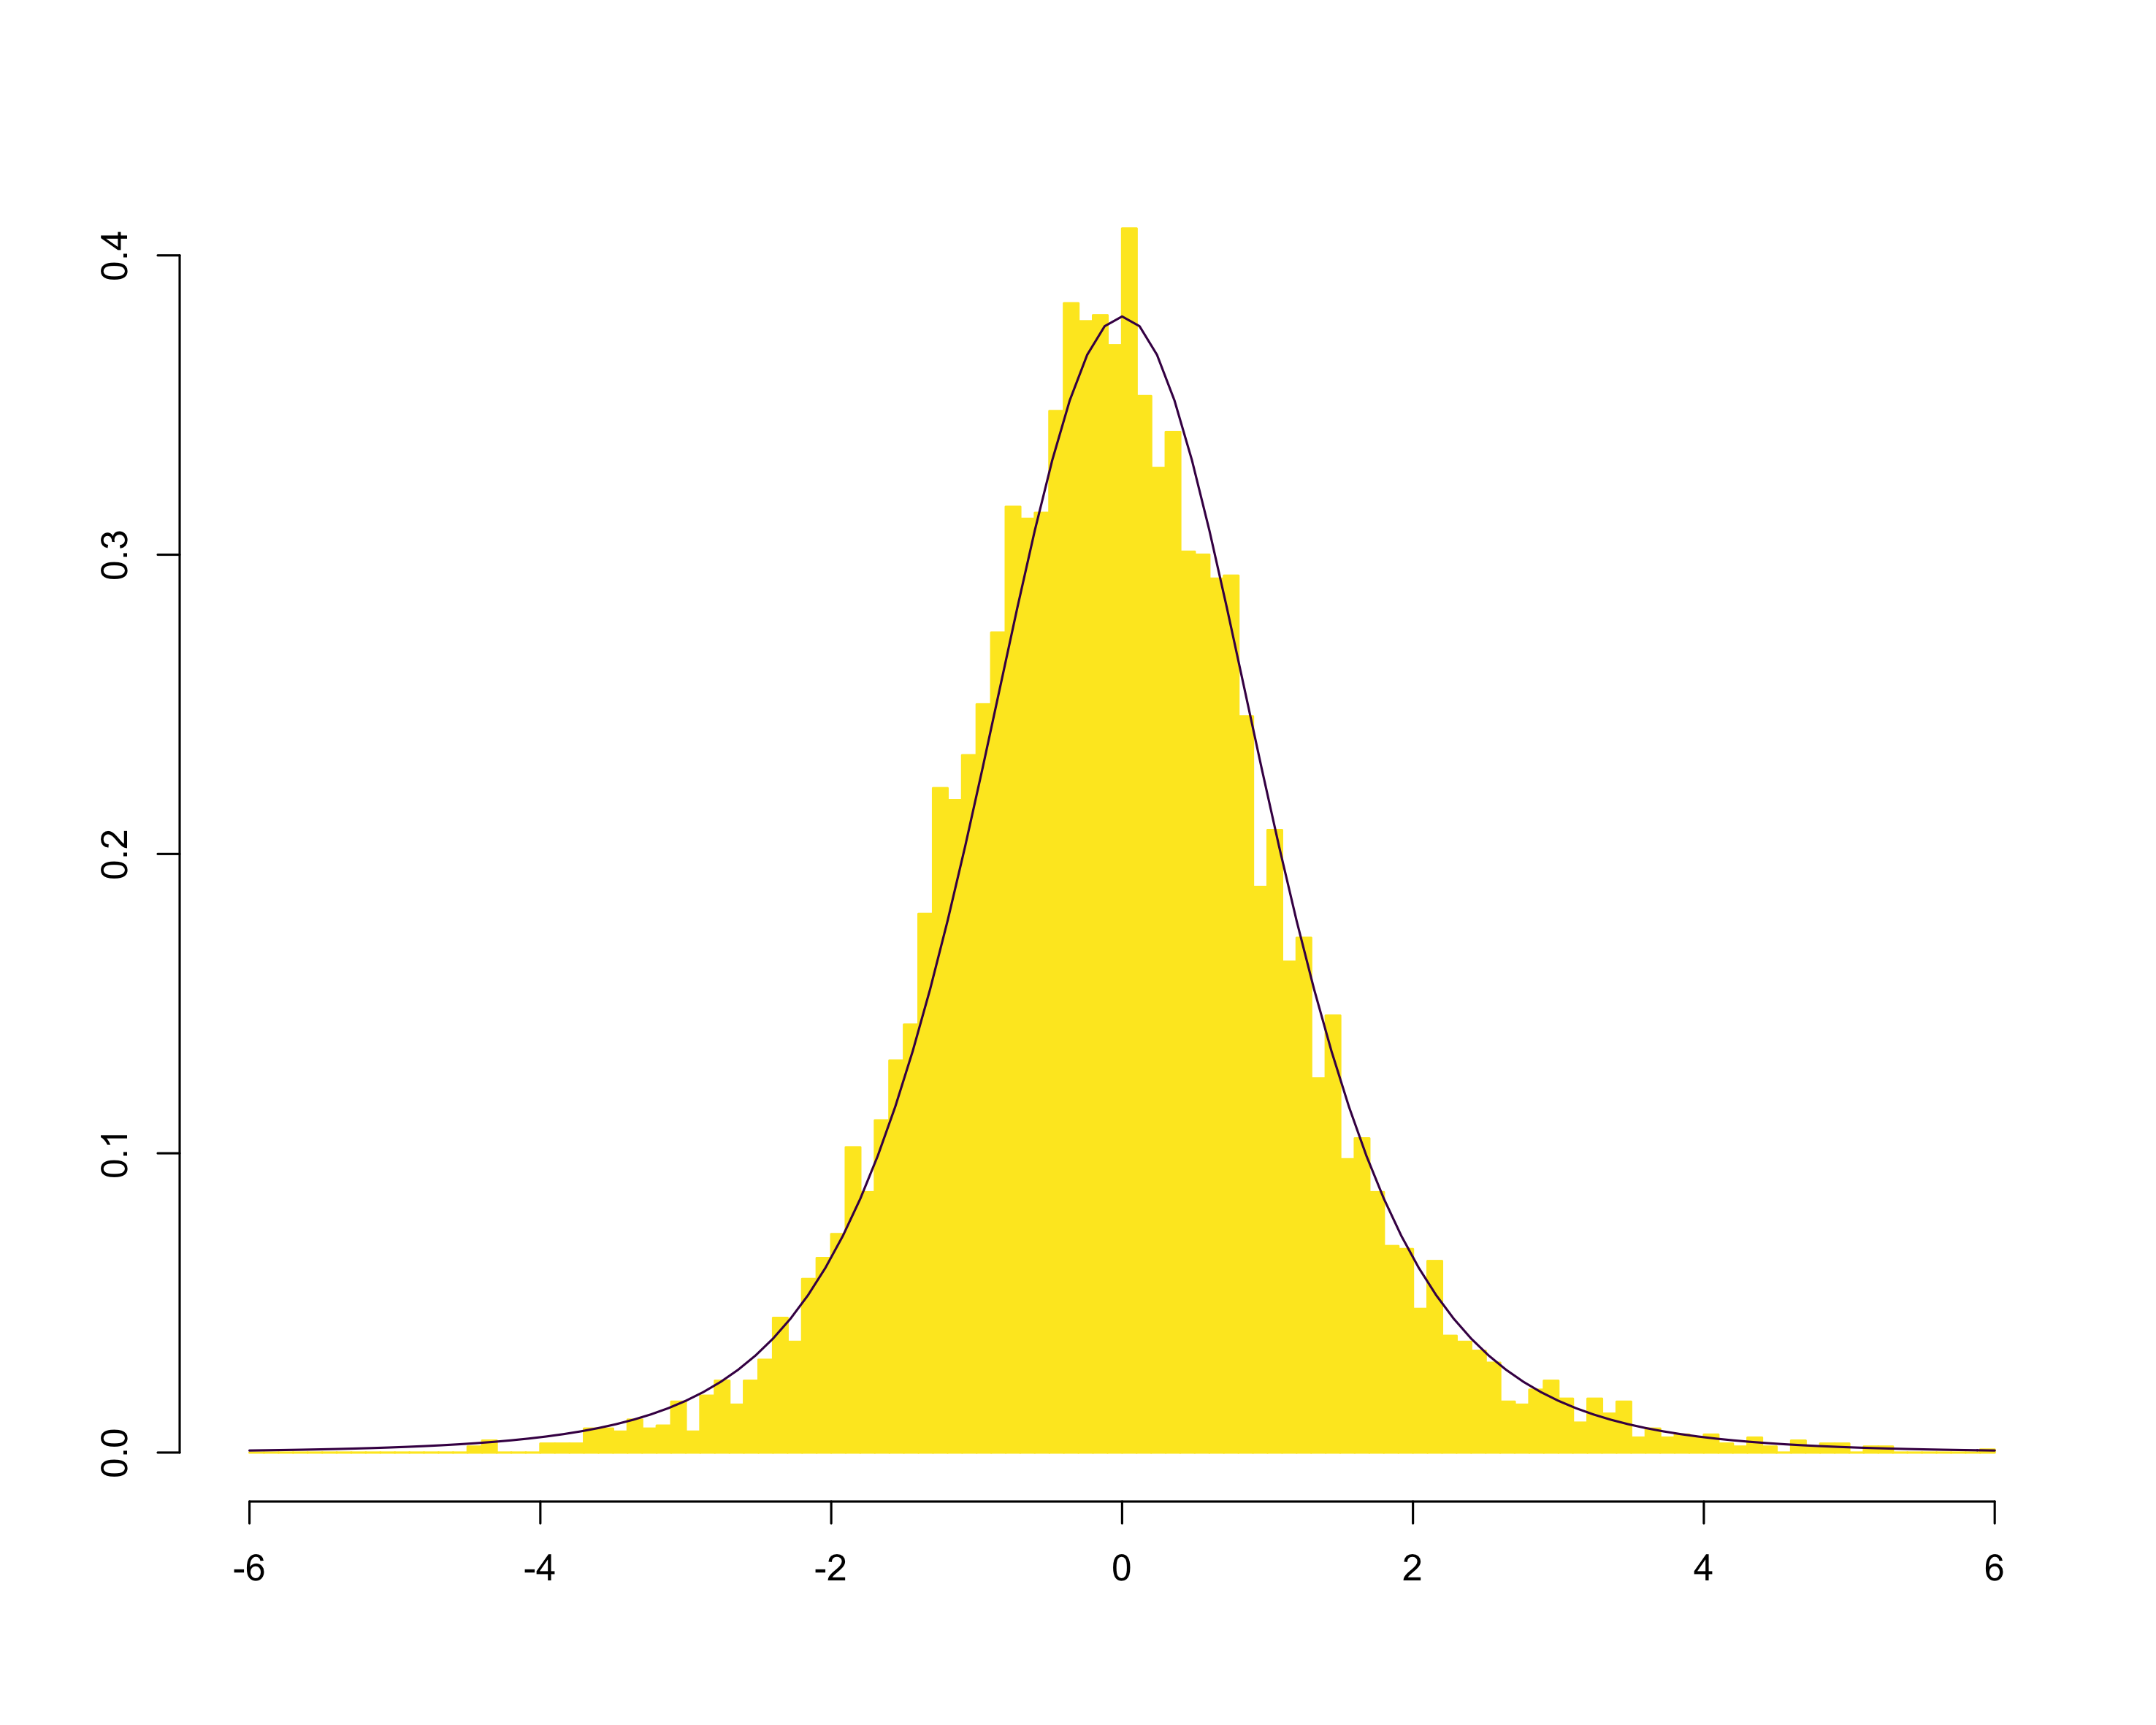
\includegraphics[width=\linewidth]{mh_hist_x3.png} 
        \caption{Histograma de $f \sim t_{(5)}$ con propuestas $q_3$} \label{fig:mh_hist_x3}
    \end{subfigure}
    \hfill
    \begin{subfigure}[t]{0.45\textwidth}
        \centering
        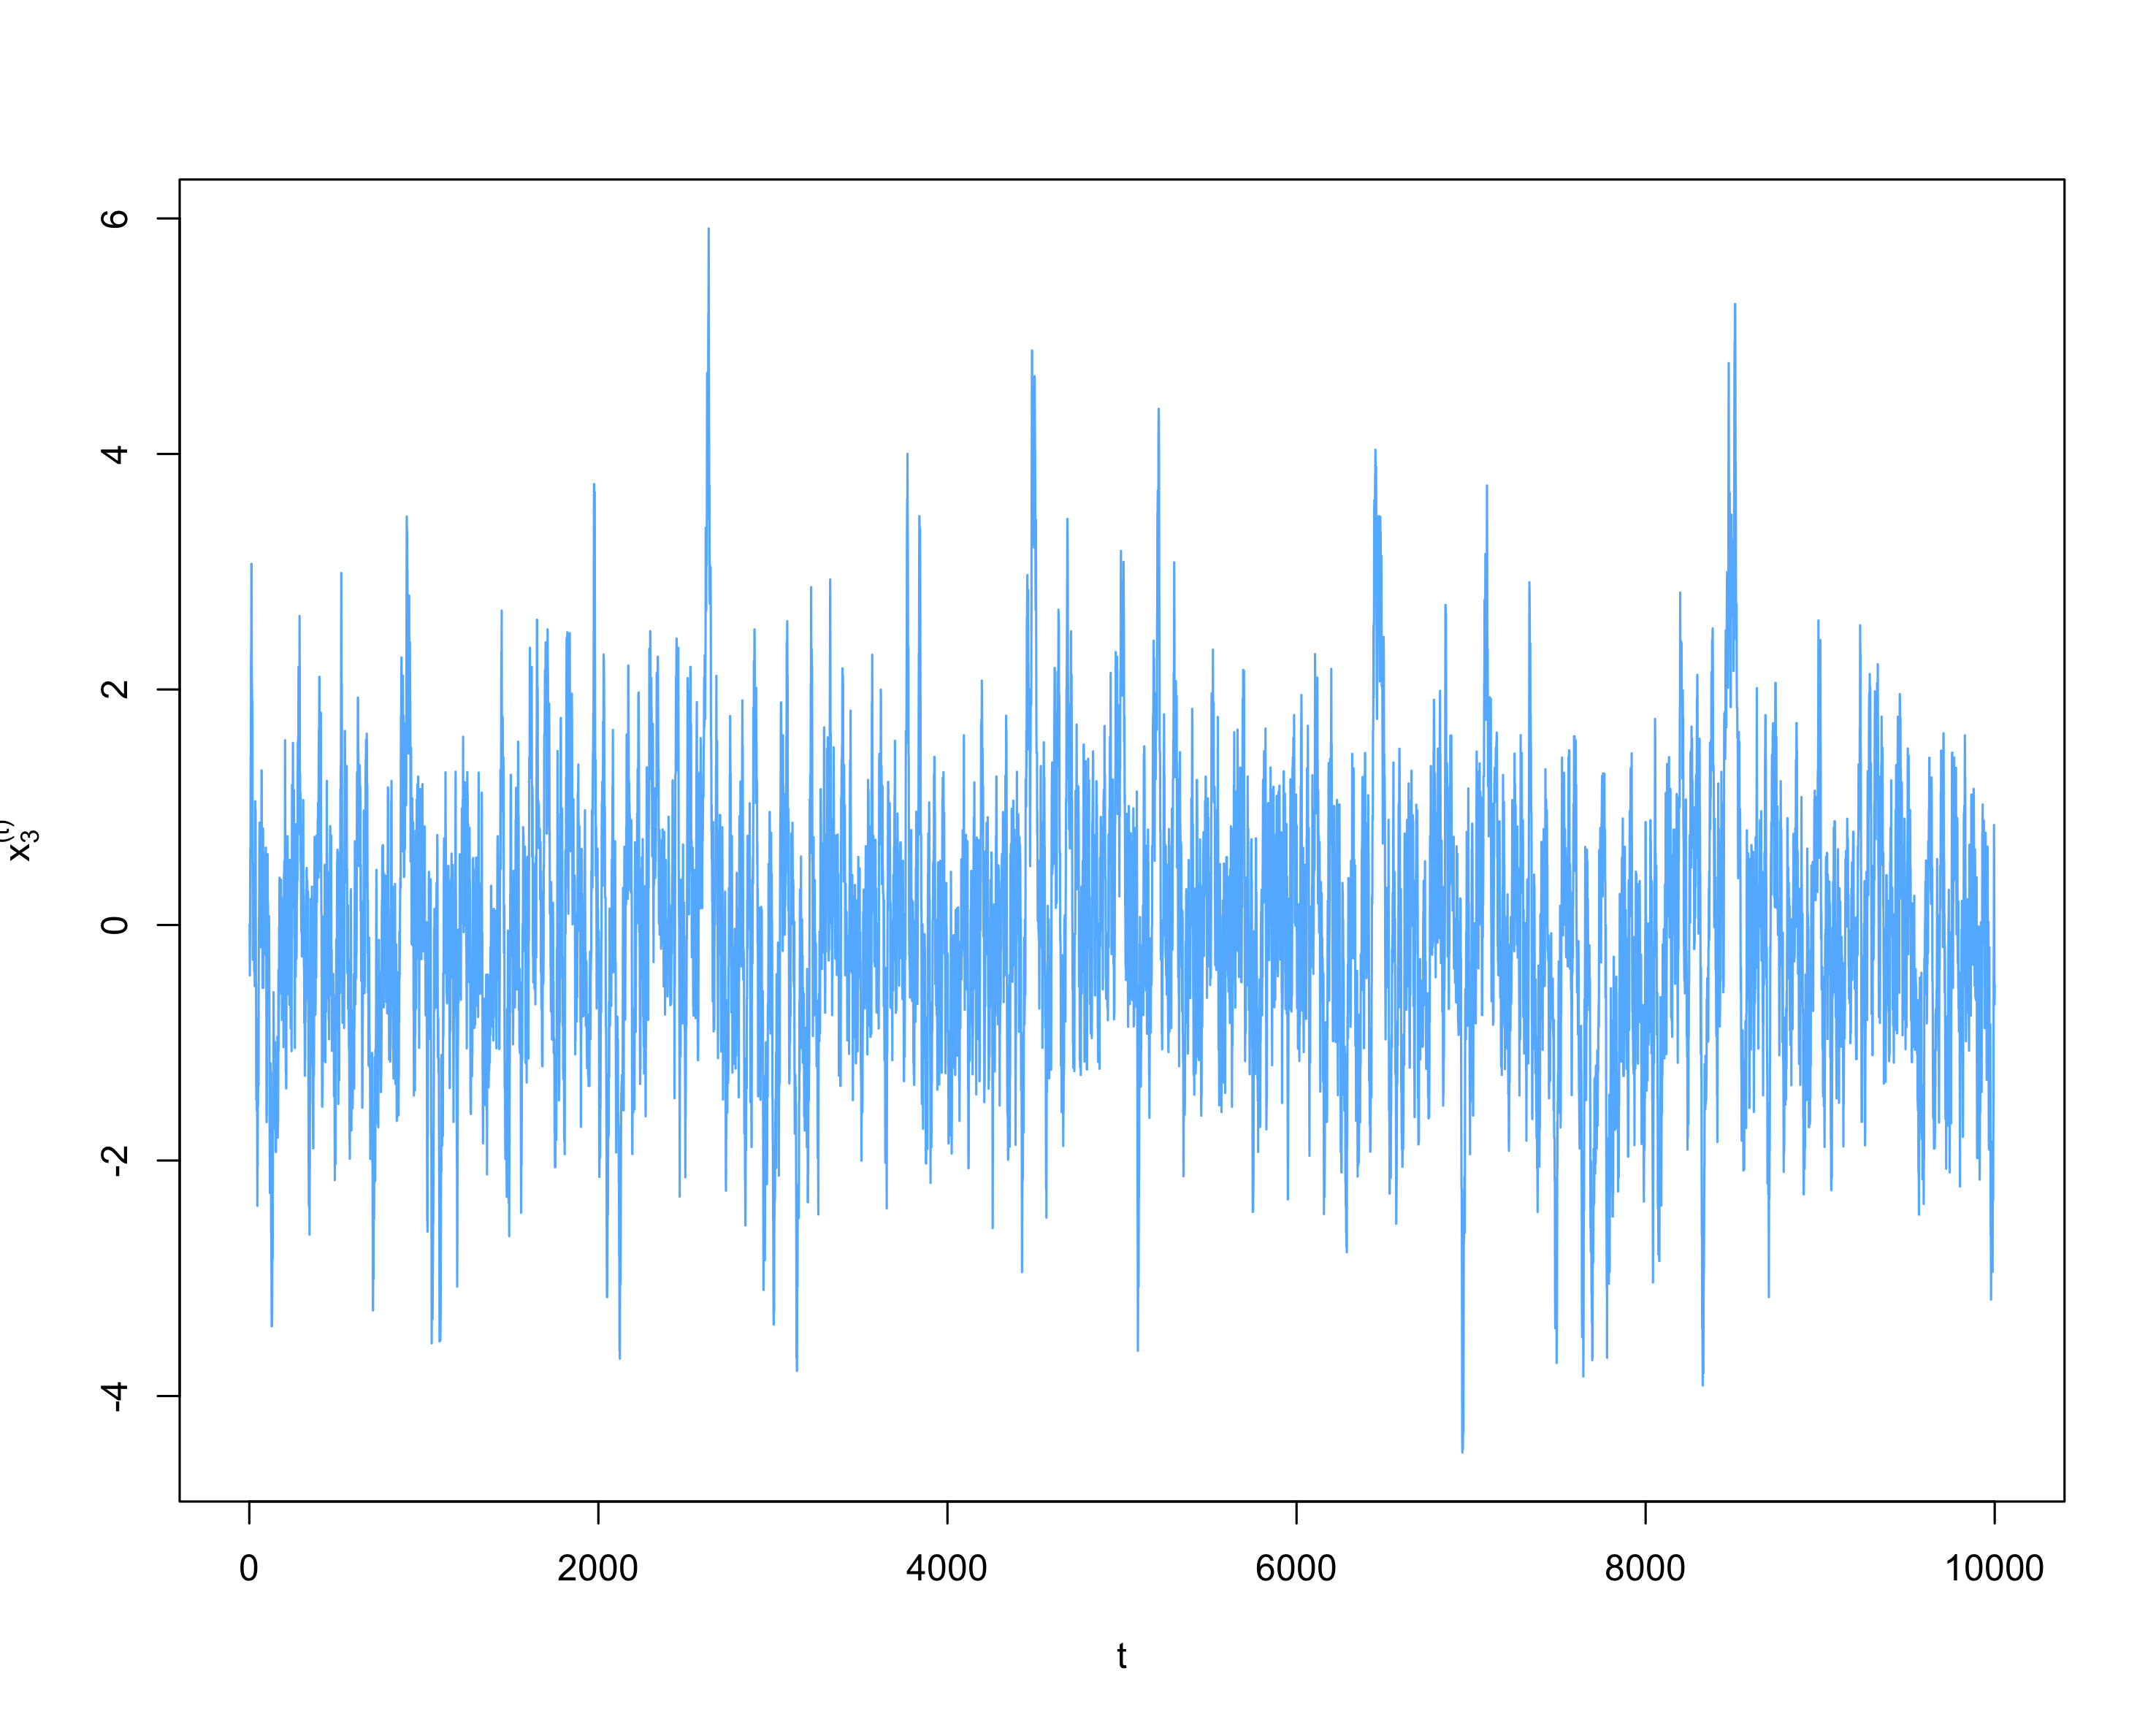
\includegraphics[width=\linewidth]{mh_chain_x3.png} 
        \caption{Proceso $\lbrace X_t^3 \rbrace$} \label{fig:mh_chain_x3}
    \end{subfigure}
    
    \caption{Simulaciones de $f \sim t_{(5)}$ utilizando el algoritmo de Metropolis-Hastings con propuestas $q_1$, $q_2$ y $q_3$}
    \label{fig:mh_t}
\end{figure}

Podemos ver en la figura \ref{fig:mh_t} que los tres histogramas parecen ajustarse bien a la distribución $t_{(5)}$, aunque hay algunas diferencias notables. Primero, la cadena con propuestas de la distribución normal estándar es la que tiene un rango más reducido de observaciones, más o menos entre -4 y 4. Esto tiene sentido ya que la distribución normal tiene colas más ligeras que la $t$, por lo que al proceso le cuesta más explorar valores alejados de la media. Por el contrario, las cadenas con propuestas $q_2$ y $q_3$ abarcan intervalos más amplios. Específicamente, las propuestas con la caminata aleatoria normal son las que exploran un mayor rango de la distribución de interés, alrededor del intervalo $(-6, 6)$.\\

A pesar de las diferencias mencionadas arriba, no es obvio a simple vista cuál de las cadenas funciona mejor para simular observaciones de la distribución $t_{(5)}$. Para poder elegir la distribución $q$ debemos tener criterios de selección, basados en diagnósticos de las cadenas. Ahora introducimos algunos diagnósticos comunes.\\

Hay tres cosas que debemos monitorear en muestras de MCMC \citep{kruschke}:
\begin{enumerate}
\item Convergencia de la cadena a la distribución estacionaria.\\
\item Precisión y estabilidad de nuestras estimaciones (valores esperados, cuantiles, etc.).
\item Eficiencia en las simulaciones.\\
\end{enumerate}

Diagnosticar la convergencia a la distribución estacionaria suele ser complejo porque en muchas aplicaciones se desconoce la geometría de la distribución de interés. Por esto, es común utilizar diagnósticos visuales de los estados que visita la cadena en cada iteración. La idea es generar varias cadenas con estados iniciales distintos. Buscamos que después de cierto número de iteraciones, las distintas cadenas estén explorando la misma región de la distribución de interés, eliminando la dependencia de los valores iniciales. A estas gráficas se les llama de traza o \textit{trace plots.}\\

Es esencial que este diagnóstico visual utilice múltiples cadenas, ya que si solamente se toma una cadena podemos tener la falsa idea de que la cadena explora de manera eficiente el rango de la distribución. Un ejemplo es si la distribución de interés es bimodal y nuestra cadena explora solamente la vecindad de una de las modas. Es una condición necesaria, más no suficiente de convergencia a la distribución estacionaria que al visualizar las cadenas en la misma gráfica, éstas se encimen y exploren la misma región.\\

Otra visualización que se puede utilizar para este diagnóstico son suavizamientos de los histogramas. Cuando las cadenas convergen a la distribución estacionaria, sus histogramas deben ser parecidos. El suavizamiento se hace para facilitar la visualización simultánea de distintas cadenas.\\

Es una práctica común \citep{kruschke}, \citep{gelman}, \citep{casella} que se descarten las primeras iteraciones de los algoritmos para eliminar la dependencia de los valores iniciales. A estas observaciones descartadas se les llama período de calentamiento o \textit{burn-in}. No existe una regla universal que nos diga cuál es la longitud necesaria de \textit{burn-in}. Ésta se debe elegir examinando los \textit{trace plots} de las cadenas.\\

Finalmente, un diagnóstico numérico que se puede utilizar es la varianza dentro y entre cadenas. La idea de este diagnóstico es que, si una cadena no explora el rango completo de la distribución objetivo, entonces la varianza de esa cadena va a subestimar la varianza de la distribución, aproximándose a la verdadera varianza en el límite. Esto se compara con un promedio ponderado de las varianzas dentro y entre cadenas, el cual es un estimador insesgado de la varianza de la distribución objetivo cuando las observaciones vienen de ésta \citep{gelman}.\\

Respecto a la precisión y estabilidad de las cantidades estimadas, es muy importante recalcar que las observaciones simuladas con los algoritmos de MCMC no son independientes. Esto significa que los algoritmos de MCMC no exploran la distribución objetivo de manera tan eficiente como lo hacen los algoritmos de la sección \ref{simulacion}. Específicamente, mientras mayor sea la correlación entre observaciones, menor es la eficiencia en la exploración. Para diagnosticar esto, se utilizan gráficos de autocorrelación. Estas figuras muestran la correlación que hay entre los valores de la cadena y esos mismos valores desplazados $k$ períodos.\\

También existe un diagnóstico numérico para cuantificar el efecto de la correlación en las observaciones. Se le conoce como tamaño de muestra efectivo o \textit{effective sample size} e intuitivamente nos dice el tamaño de muestra que necesitaríamos para obtener la misma información si nuestras observaciones se generaran de manera independiente \citep{kruschke}.\\

Finalmente, es recomendable que nuestras simulaciones sean lo más eficientes posible. Es decir, que tengamos la mayor cantidad de información en el menor tiempo. Esto se puede lograr explorando distintas opciones al seleccionar algoritmos y distribuciones candidatas, al igual que realizando simulaciones en paralelo y explotando al máximo los recursos computacionales a nuestro alcance.\\

Todavía no vamos a ejemplificar los diagnósticos mencionados en este capítulo. Lo haremos hasta que exploremos los resultados del modelo en el capítulo \ref{elmodelo}. Por el momento, sepa el lector que la mayoría (si no es que todos) estos diagnósticos están disponibles en el paquete \texttt{coda} de R \citep{coda}, el cual se puede instalar fácilmente con el comando \texttt{install.packages(``coda")}.\\

Antes de cerrar este capítulo, sepa el lector que distintos algoritmos de MCMC, además del muestreador de Gibbs y Metropolis-Hastings, se han desarrollado y son cada vez más comunes en la comunidad estadística (mientras se escribe este trabajo). Especialmente hay que resaltar los algoritmos de Monte Carlo Hamiltoniano, los cuales utilizan nociones físicas y de sistemas dinámicos para explorar de manera eficiente las distribuciones. Estos métodos son especialmente útiles en grandes dimensiones porque incorporan información de la geometría de la distribución. El uso de Monte Carlo Hamiltoniano ha ido en aumento en gran parte gracias al software Stan \citep{stan}, el cual implementa este algoritmo y cuenta con interfaces para algunos de los lenguajes de programación más populares como R y Python.\\

Profundizar más en este tema está completamente fuera del alcance de este trabajo. El interesado (y atrevido) lector puede consultar más sobre Monte Carlo Hamiltoniano en \citet{neal}, \citet{betancourt}, \citet{gelman}. Para mayor información sobre Stan se recomienda consultar \citet{gelman}, \citet{kruschke} y el sitio web \url{https://mc-stan.org} que contiene manuales e información de libre acceso. Ahora que terminamos de construir el esqueleto con los preliminares, pasemos a la carnita del asunto con el modelo que nos incumbe.\\

\section{El modelo}
\label{elmodelo}

El artículo \citet{nieto} introduce un modelo bayesiano semiparamétrico para estudiar tiempos de supervivencia multivariados. En este capítulo se explica la construcción del modelo, enfocándonos únicamente en el caso bivariado.\\

El objetivo es construir un modelo capaz de lidiar con la correlación entre tiempos de fallo de manera adecuada, manteniendo esta estructura de dependencia simple y utilizando densidades marginales no paramétricas para que sean lo más flexibles posible.\\

\subsection{Caso univariado}

Para introducir las ideas, veamos el caso univariado. Sea $T$ una variable aleatoria con soporte $S_T = [0, \infty)$ y sean $h$ y $H$ la función de riesgo y riesgo acumulado respectivamente. Nos interesa escribir la función de densidad $f$ como una mezcla de la forma
\begin{equation} \label{mezcla}
f(t) = \int_\Omega f(t|\omega)m(\omega) \ d\omega,
\end{equation}
donde $\Omega$ es el soporte de $\omega$. El resultado siguiente muestra que se puede escribir $f(t)$ de la forma \eqref{mezcla}.

\begin{proposition}
Sean $f(t|\omega) = \frac{h(t)}{\omega} \ \mathbb{I}\lbrace\omega > H(t)\rbrace$ y $m(\omega)\sim Ga(\omega \ | \ 2, 1)$. Entonces se cumple la representación como mezcla dada por \eqref{mezcla}.
\end{proposition}

\begin{proof}
\begin{align*}
m(\omega) \sim Ga(\omega \ | \ 2, 1) &\implies m(\omega) = \omega e^{-\omega} \ (\omega\geq 0)\\
&\implies f(t|\omega) = h(t)e^{-\omega} \ \mathbb{I}\lbrace\omega > H(t)\rbrace.
\end{align*}

Así,
\begin{align*}
\int_\Omega f(t|\omega)m(\omega) \ d\omega &= \int_{H(t)}^\infty h(t)e^{-\omega} \ d\omega\\
&= h(t) \exp(-H(t))\\
&= h(t)S(t)\\
&= f(t).\\
\end{align*}
\end{proof}

El objetivo es utilizar esta representación como mezcla para introducir la estructura de dependencia a través de densidades $Ga(2, 1)$ y no a través de las funciones de densidad arbitrarias $f(t)$.

\subsection{Caso bivariado} \label{caso_bivariado}
Sea ahora $T=(T_1, T_2)$ un vector aleatorio con soporte $S_T = [0, \infty) \times [0, \infty)$ y función de densidad conjunta $f(t_1, t_2)$. Generalizando la idea \eqref{mezcla}, escribimos la densidad conjunta como
\begin{equation} \label{mezcla_conjunta}
f(t_1, t_2) =\int_\Omega\int_\Omega f(t_1, t_2 \ | \ \omega_1, \omega_2)m(\omega_1, \omega_2) \ d\omega_1 d\omega_2.\\
\end{equation}

Del modelo univariado sabemos que las densidades marginales se pueden escribir como en \eqref{mezcla} con
\begin{equation} \label{marginal}
f_j(t|\omega_j) = \frac{h_j(t)}{\omega_j} \ \mathbb{I}\lbrace\omega_j > H(t)\rbrace
\end{equation}
y $\omega_j \sim Ga(2, 1)$.\\

Ahora asumimos independencia condicional dada $\omega = (\omega_1, \omega_2)$, es decir,
\begin{equation} \label{indcon}
f(t_1, t_2 \ | \ \omega_1, \omega_2) = f(t_1 | \omega_1)f(t_2 | \omega_2)\\
\end{equation}
y que $\omega = (\omega_1, \omega_2)$ tiene una distribución gamma bivariada con marginales $Ga(2, 1).$\\

De esta manera, la construcción definida en las ecuaciones (\ref{mezcla_conjunta} - \ref{indcon}) garantiza que $T_1$ y $T_2$ tienen distribuciones marginales con función de riesgo $h_1(t)$ y $h_2(t)$ respectivamente. Además, la dependencia entre ellos es modelada a través de la dependencia entre $\omega_1$ y $\omega_2$.\\

El siguiente resultado muestra que la construcción definida en las ecuaciones (\ref{mezcla_conjunta} - \ref{indcon}) define una cópula de supervivencia.

\begin{proposition}
La función de supervivencia conjunta obtenida a través de las ecuaciones (\ref{mezcla_conjunta} - \ref{indcon}) define una cópula de supervivencia, esto es, $$S(t_1, t_2) = C(S_1(t_1), S_2(t_2)),$$ donde la cópula $C$ es la función dada por
\begin{equation} \label{copula_modelo}
C(u, v) = \int_{-\log (u)}^\infty \int_{-\log (v)}^\infty \left(1 + \frac{\log(u)}{\omega_1}\right)\left(1 + \frac{\log(v)}{\omega_2}\right) m(\omega_1, \omega_2) \ d\omega_1 d \omega_2.
\end{equation}
\end{proposition}

El curioso lector puede encontrar la construcción de la cópula en el apéndice \ref{construccion_copula}. ¡No se encuentra en el artículo original!\\

La utilidad de este resultado recae en que podemos estudiar las medidas de concordancia introducidas en la sección \ref{sec_copulas} sin especificar las distribuciones marginales. Como las integrales que definen $\uptau$ y $\rho$ no se pueden resolver analíticamente, utilizamos las técnicas de integración Monte Carlo introducidas en la sección \ref{sec_cadenas} para aproximarlas.\\

Ya que las expresiones para $\uptau$ y $\rho$ las obtuvimos para cópulas de distribución (no de supervivencia), trabajaremos ahora con esta forma, la cual está dada por la expresión
\begin{align}\label{copula_distribucion}
C(u, v) &= u \ + \ v \ - \ 1 \ +\nonumber\\ 
& \ \ \ \int_{-\log (1-u)}^\infty \int_{-\log (1-v)}^\infty f(u, v, \omega_1, \omega_2) \ d\omega_2 d\omega_1,
\end{align}

donde $f(u, v, \omega_1, \omega_2) = \left( \frac{\log (u)}{\omega_1}+1 \right) \left( \frac{\log (v)}{\omega_2}+1\right) m(\omega_1, \omega_2)$.\\

La cópula \eqref{copula_distribucion} tiene densidad dada por
\begin{align}
\partial c(u, v) &= \frac{\partial^2C}{\partial v \partial u}\nonumber\\
&= \int_{-\log (1-u)}^\infty \int_{-\log (1-v)}^\infty \frac{m(\omega_1, \omega_2)}{(1-u)(1-v)\omega_1\omega_2} \ d\omega_2 d\omega_1 \nonumber\\
&= E_{m} \left[\frac{\mathbb{I}\lbrace u < 1-e^{-\omega_1}\rbrace \mathbb{I}\lbrace v < 1-e^{-\omega_2} \rbrace}{(1-u)(1-v)\omega_1\omega_2}\right],
\end{align}
donde $E_m$ es el valor esperado con respecto a la distribución $m(\omega_1, \omega_2)$. El desarrollo de esta expresión se puede encontrar en el apéndice \ref{sec_densidad_copula_modelo}.\\

Recordemos las expresiones de la tau de Kendall y la rho de Spearman para una cópula $\mathcal{C}$:
\begin{itemize}
\item $\uptau_{\mathcal{C}} = 4\int_{0}^1\int_{0}^1\C(u, v) \ d\C(u, v) - 1,$\\
\item $\rho_{\mathcal{C}} = 12\int_0^1 \int_0^1 C(u, v) \ dudv-3.$\\
\end{itemize}

Podemos reescribir estas integrales como valores esperados y utilizar integración Monte Carlo para aproximarlas:
\begin{equation} \label{tau_esperado}
\uptau_{\mathcal{C}} = 4 \ E_{(U, V)}\left[C(u, v) \partial c(u, v)\right] -1,
\end{equation}
\begin{equation} \label{rho_esperado}
\rho_{\mathcal{C}} = 12 \ E_{(U, V)}\left[C(u, v)\right] -3,
\end{equation}
donde $E_{(U, V)}$ es el valor esperado respecto a una densidad uniforme en \newline $(0, 1)\times (0, 1).$\\

A continuación escribimos también la integral de la cópula \eqref{copula_distribucion} como un valor esperado.
\begin{align*}
&C(u, v) = u \ + \ v \ - \ 1 \ +\\
& \ \ \ E_{m} \left[\mathbb{I}\lbrace u < 1-e^{-\omega_1}\rbrace \mathbb{I}\lbrace v < 1-e^{-\omega_2}\rbrace \left(1 + \frac{\log (1-u)}{\omega_1}\right)\left(1 + \frac{\log (1-v)}{\omega_2}\right)\right],
\end{align*}
lo cual nos permitirá aproximarla a su vez con integración Monte Carlo.\\

Lo único que falta para realizar las aproximaciones es especificar la distribución $m(\omega_1, \omega_2)$ para simular observaciones y aproximar las integrales. En el artículo \citet{nieto} se introduce esta distribución de la siguiente forma.\\

Tomamos
\begin{align*}
\omega_j | y &\sim Ga(a + y, b + \gamma)\\
y &\sim Pg(a, b, \gamma),
\end{align*}
donde $Pg$ se refiere a la distribución Poisson-gamma introducida en la sección \ref{sec:transformada}.\\

Con esta definición se tiene que el vector aleatorio $(\omega_1, \omega_2)$ tiene una distribución gamma bivariada con parámetros $a, b, \gamma > 0$, denotada $BGa(a, b, \gamma)$. Marginalmente, $\omega_j \sim Ga(a, b)$ y se tiene además que $$corr(\omega_1, \omega_2) = \frac{\gamma}{b + \gamma}.$$

Los autores resaltan que esta construcción solamente permite una correlación positiva entre $\omega_1$ y $\omega_2$. En caso de requerir correlación negativa se necesitaría utilizar una distribución gamma bivariada distinta.\\

Ahora, como en \eqref{marginal} requerimos que las $\omega_j$ tengan una distribución $Ga(2, 1)$, se tiene que 
\begin{align} \label{eq_omegas}
\omega_j | y &\sim Ga(2 + y, 1 + \gamma) \nonumber\\
y &\sim Pg(2, 1, \gamma)\\
\text{y } corr(\omega_1, \omega_2) &= \frac{\gamma}{1 + \gamma}. \nonumber
\end{align}
Así, el único parámetro que necesitamos para definir la distribución es $\gamma$ y tenemos que $(\omega_1, \omega_2) \sim BGa(2, 1, \gamma), \ \gamma >0$. Con esta construcción de $m(\omega_1, \omega_2)$, podemos ya realizar las aproximaciones de $\uptau_\C$ y $\rho_\C$. Se incluyen gráficas y el código para aproximar ambas cantidades como función del parámetro $\gamma$.\\

Primero definimos dos funciones para aproximar el valor de $\C(u, v)$ y $\partial c(u, v)$.

\begin{lstlisting}

copula <- function(u, v, omega1, omega2) {
  c <- (1 + log(1 - u) / omega1) * (1 + log(1 - v) / omega2)
  c <- mean(c * (u < 1 - exp(-omega1)) * (v < 1 - exp(-omega2)))
  res <- (u + v - 1 + c) * (u > 0) * (v > 0)
  return(res)
}

\end{lstlisting}

\begin{lstlisting}
densidad_copula <- function(u, v, omega1, omega2) {
  
  c <- 1 / (1 - u) * 1 / (1 - v) * 1 / (omega1 * omega2)
  c <- mean(c * (u < 1 - exp(-omega1)) * (v < 1 - exp(-omega2)))
  
  return(c)
  
}
\end{lstlisting}

También definimos una función para obtener muestras de $m(\omega_1, \omega_2)$.

\begin{lstlisting}
sim_omega <- function(n.sim, a = 2, b = 1, gamma = 5) {
  lam <- rgamma(n = n.sim, shape = a, rate = b)
  y <- rpois(n = n.sim, lambda = lam * gamma)
  omega1 <- rgamma(n = n.sim, shape = a + y, rate = b + gamma)
  omega2 <- rgamma(n = n.sim, shape = a + y, rate = b + gamma)
  
  return(list("omega1" = omega1, "omega2" = omega2))
}

\end{lstlisting}

Ahora, realizamos la aproximación de $\uptau_\C$.

\begin{lstlisting}
n.sim <- 1e4

set.seed(42)

vec.u <- runif(n.sim)
vec.v <- runif(n.sim)

kendall_tau <- function(gamma) {
  set.seed(42)
  omega <- sim_omega(1e4, gamma = gamma)
  
  c <- vector(mode = "double", length = length(vec.u))
  dc <- vector(mode = "double", length = length(vec.u))
  
  for (i in 1:length(vec.u)) {
    u <- vec.u[i]
    v <- vec.v[i]
    c[i] <- copula(u, v, omega$omega1, omega$omega2)
    dc[i] <- densidad_copula(u, v, omega$omega1, omega$omega2)
  }
  
  return(4 * mean(c * dc) - 1)
  
}

x <- seq(from = 0, to = 100, by = 1)
y <- vector(mode = "double", length = length(x))

for (i in 1:length(x)) {
  y[i] <- kendall_tau(x[i])
}
\end{lstlisting}

\begin{figure}[H]
\centering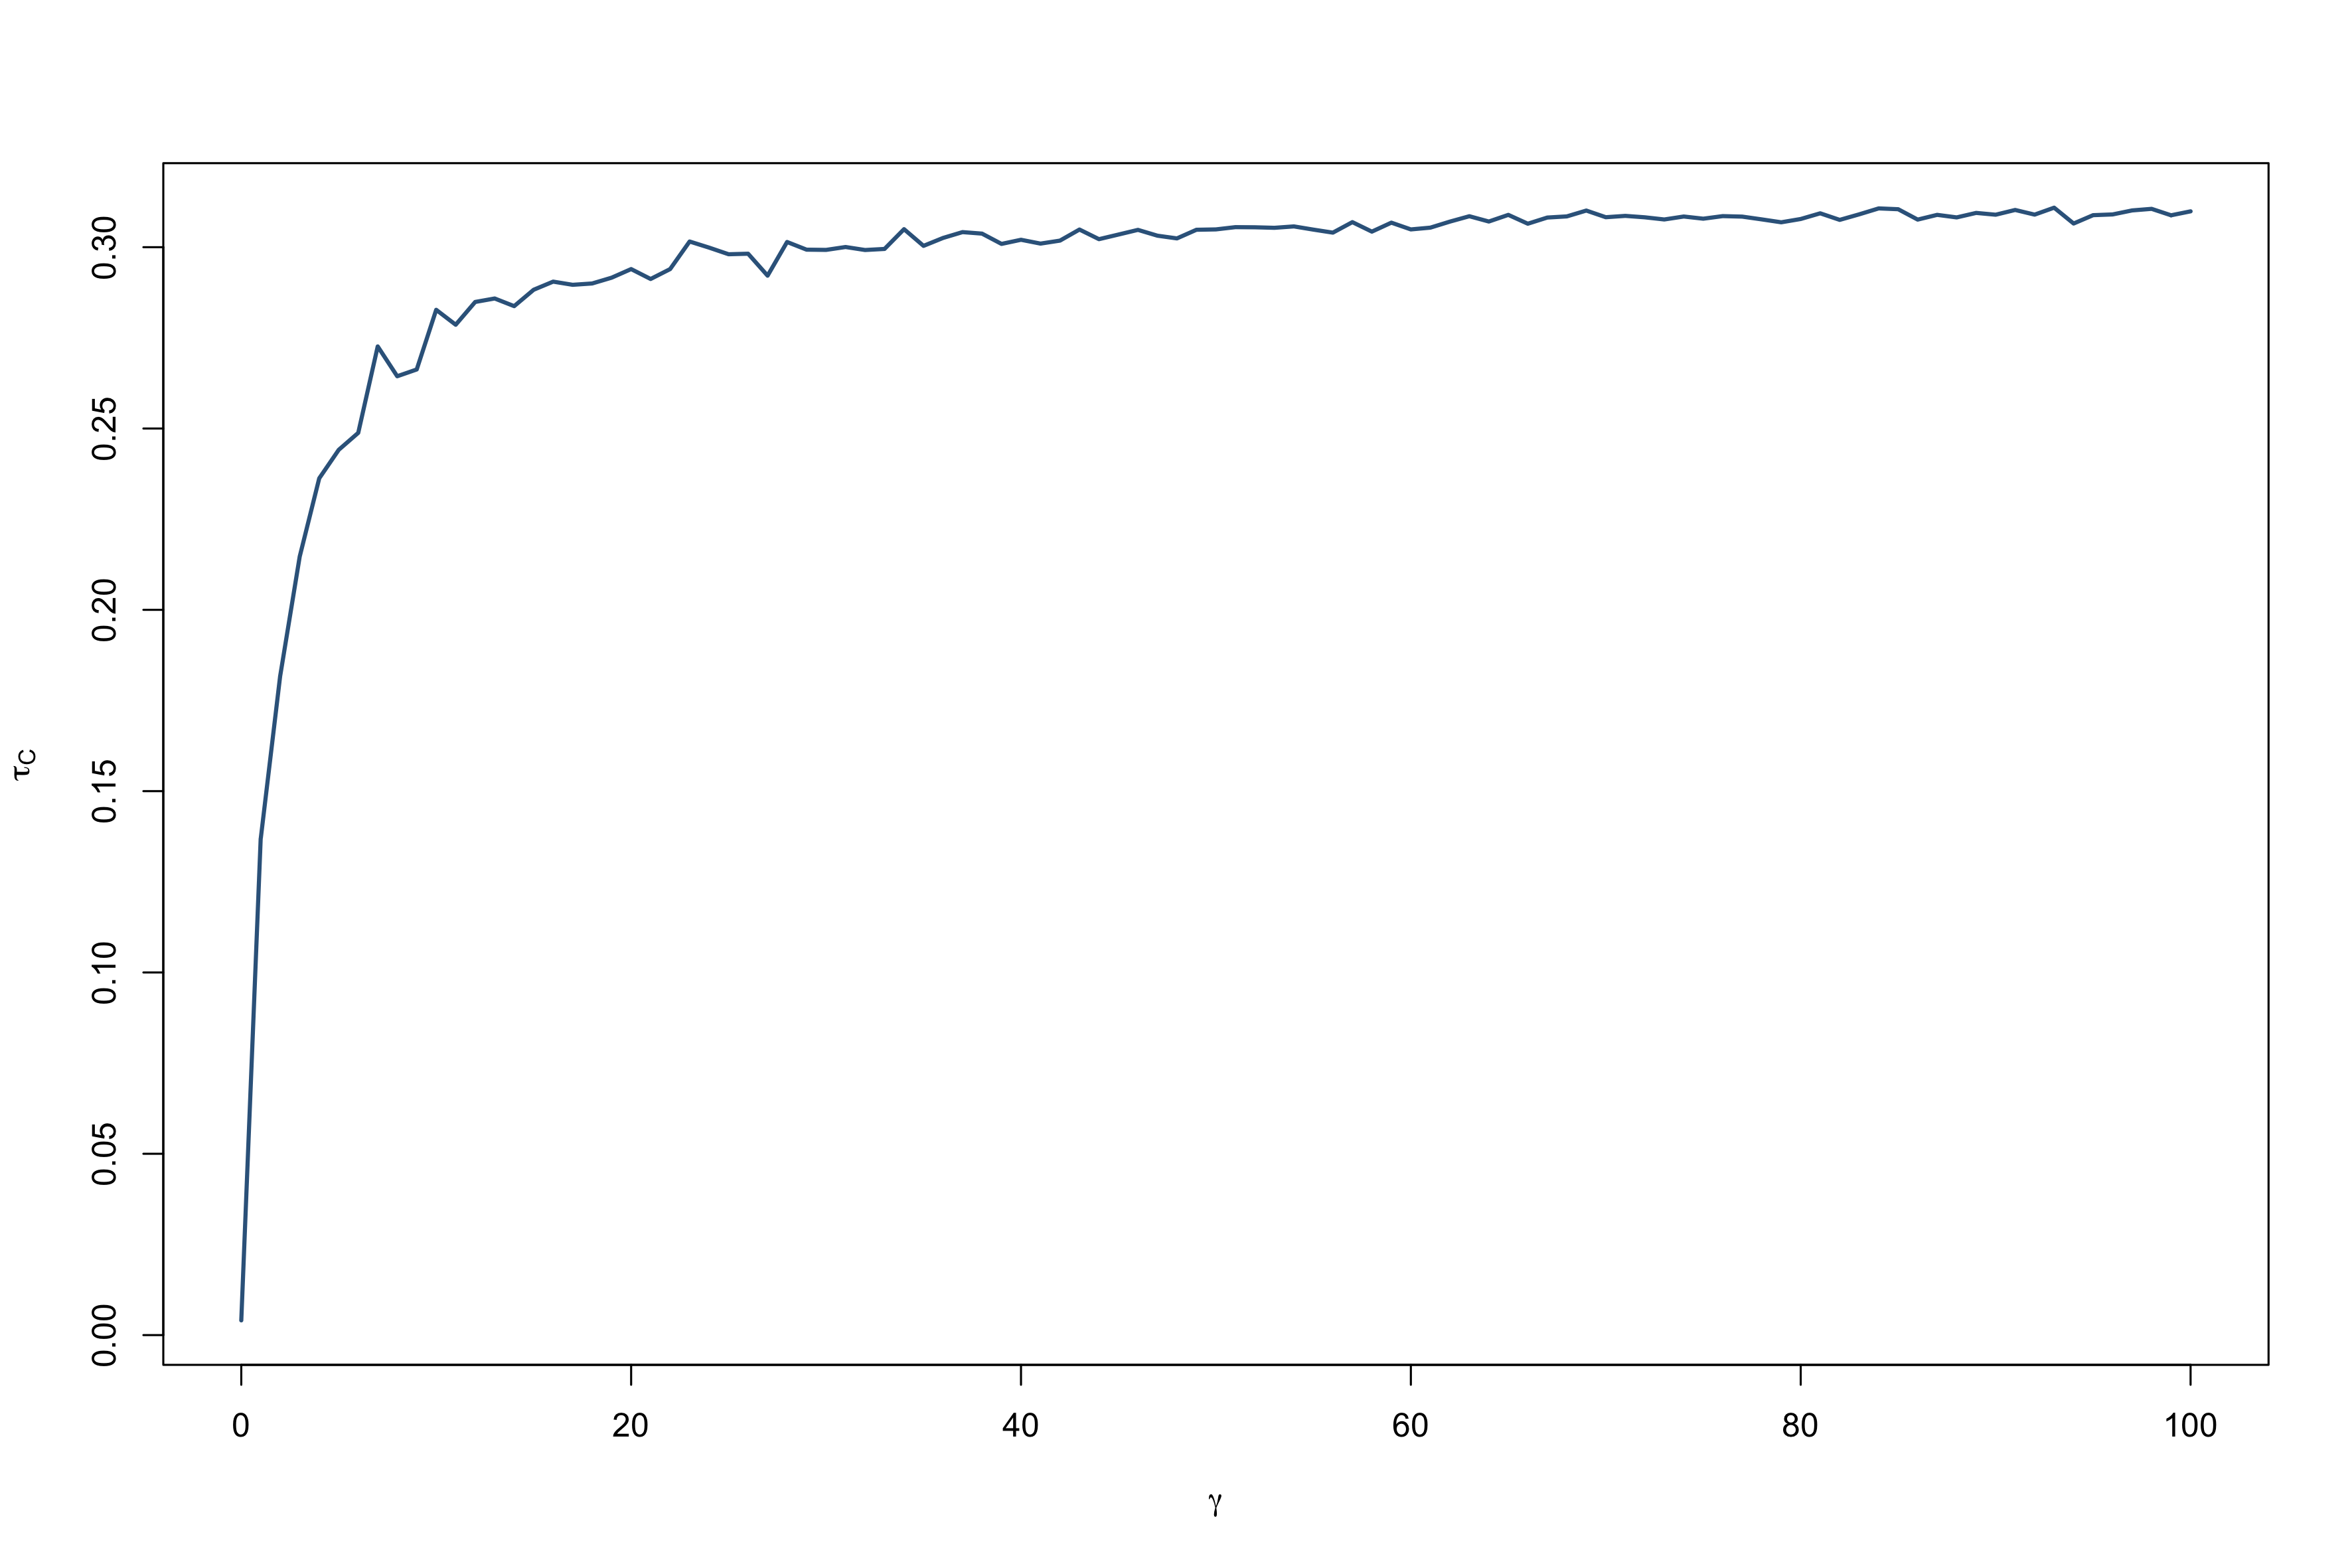
\includegraphics[width=10cm]{kendall_tau.png}
\caption{Gráfica de $\uptau_\C (\gamma)$.}
\label{fig:kendall_tau}
\end{figure}

En la figura \ref{fig:kendall_tau} podemos ver que $\uptau_\C$ es una función creciente de $\gamma$. Además, parece tener un comportamiento asintótico alrededor de $\uptau_\C = 0.3$.\\

Para la aproximación de $\rho_\C$, se utiliza la misma muestra de $(U, V)$. El código para la aproximación es el siguiente.\\

\begin{lstlisting}
spearman_rho <- function(gamma) {
  set.seed(42)
  omega <- sim_omega(1e4, gamma = gamma)
  
  c <- vector(mode = "double", length = length(vec.u))
  
  for (i in 1:length(vec.u)) {
    u <- vec.u[i]
    v <- vec.v[i]
    c[i] <- copula(u, v, omega$omega1, omega$omega2)
  }
  
  return(12 * mean(c) - 3)
  
}

rho <- vector(mode = "double", length = length(x))

for (i in 1:length(x)) {
  rho[i] <- spearman_rho(x[i])
}
\end{lstlisting}

\begin{figure}[H]
\centering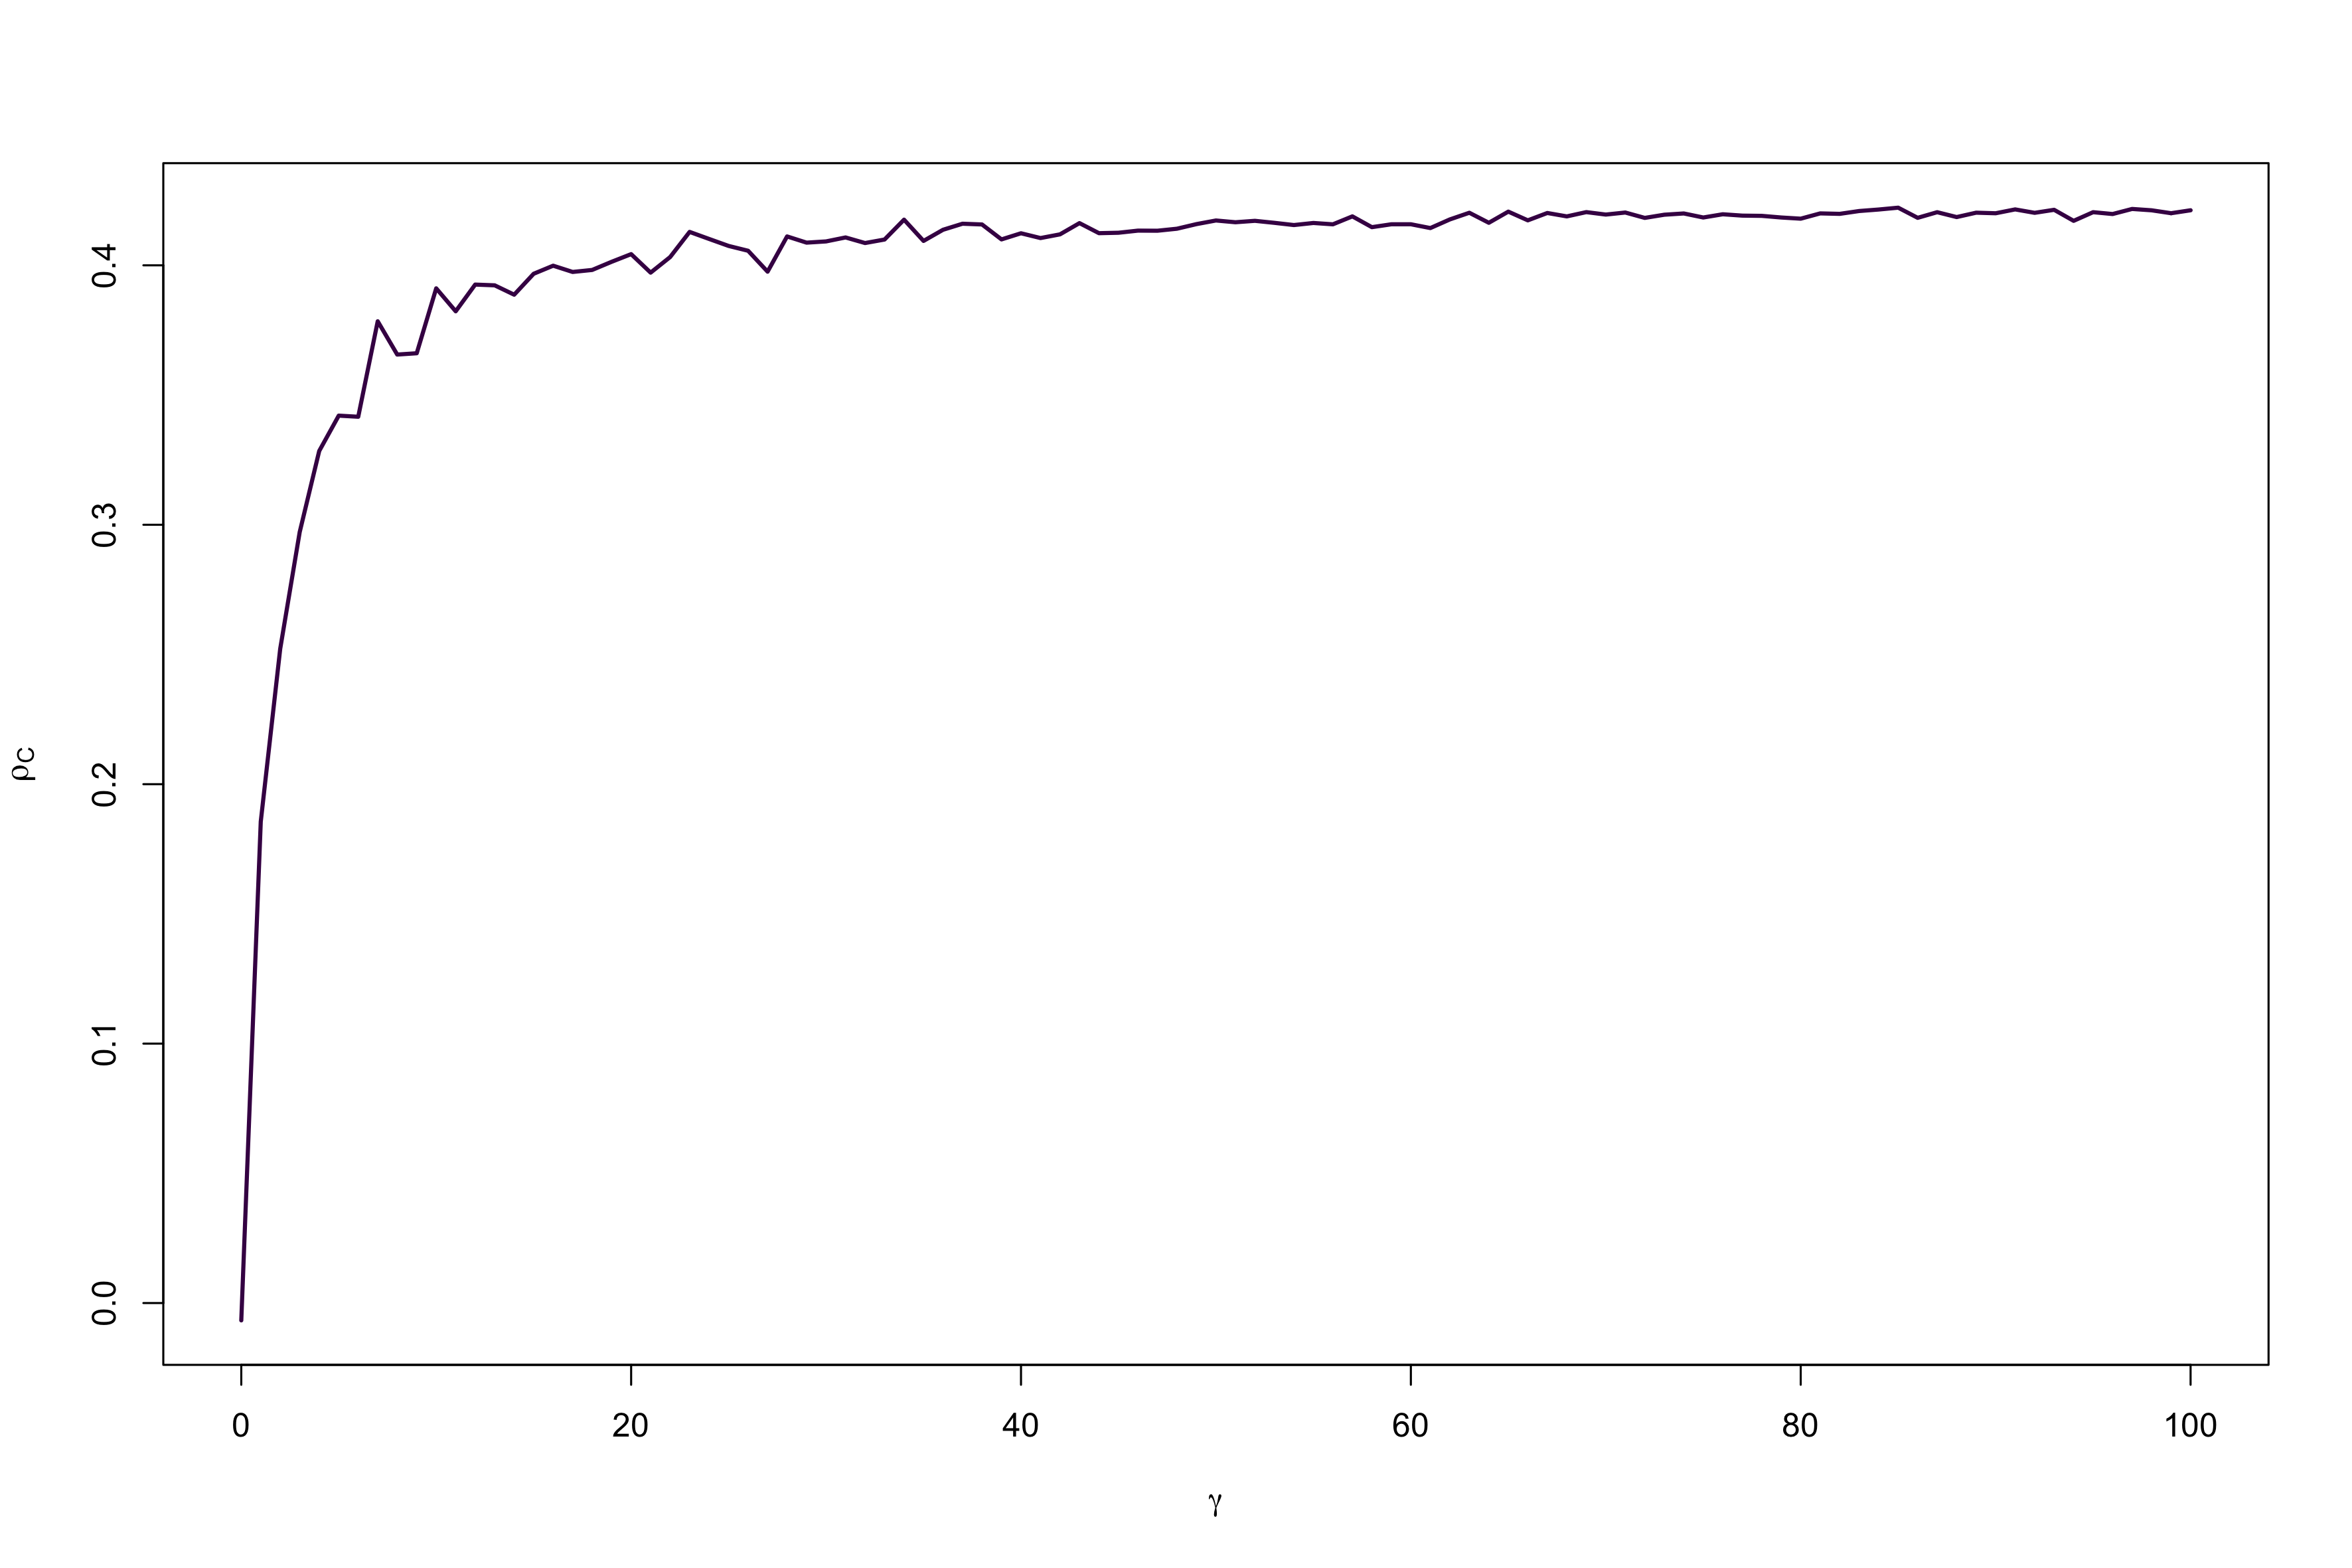
\includegraphics[width=10cm]{spearman_rho.png}
\caption{Gráfica de $\rho_\C (\gamma)$.}
\label{fig:spearman_rho}
\end{figure}

Al igual que en el caso de $\uptau_\C$, en la figura \ref{fig:spearman_rho} vemos que $\rho_\C$ es una función creciente de $\gamma$ con un comportamiento asintótico alrededor de $\rho_\C = 0.4$.\\

Por último, se presenta una gráfica de la cópula \eqref{copula_distribucion} para $\gamma = 5$. Para generar la gráfica de $\C(u, v)$, se utiliza una muestra de $m(\omega_1, \omega_2)$ para $\gamma = 5$ y la expresión de $\C$ como valor esperado para evaluar la función. El código se incluye a continuación.\\


\begin{lstlisting}

set.seed(42)

omega <- sim_omega(1e4, gamma = 1)

secuencia <- seq(from = 0.01, to = 0.99, by = 0.01)

grid <- matrix(nrow = length(secuencia), ncol = length(secuencia))

for (u in 1:length(secuencia)) {
  for (v in 1:length(secuencia)) {
    grid[u, v] <- copula(secuencia[u], secuencia[v], omega$omega1, omega$omega2)
  }
}
  
\end{lstlisting}

\begin{figure}[H]
\centering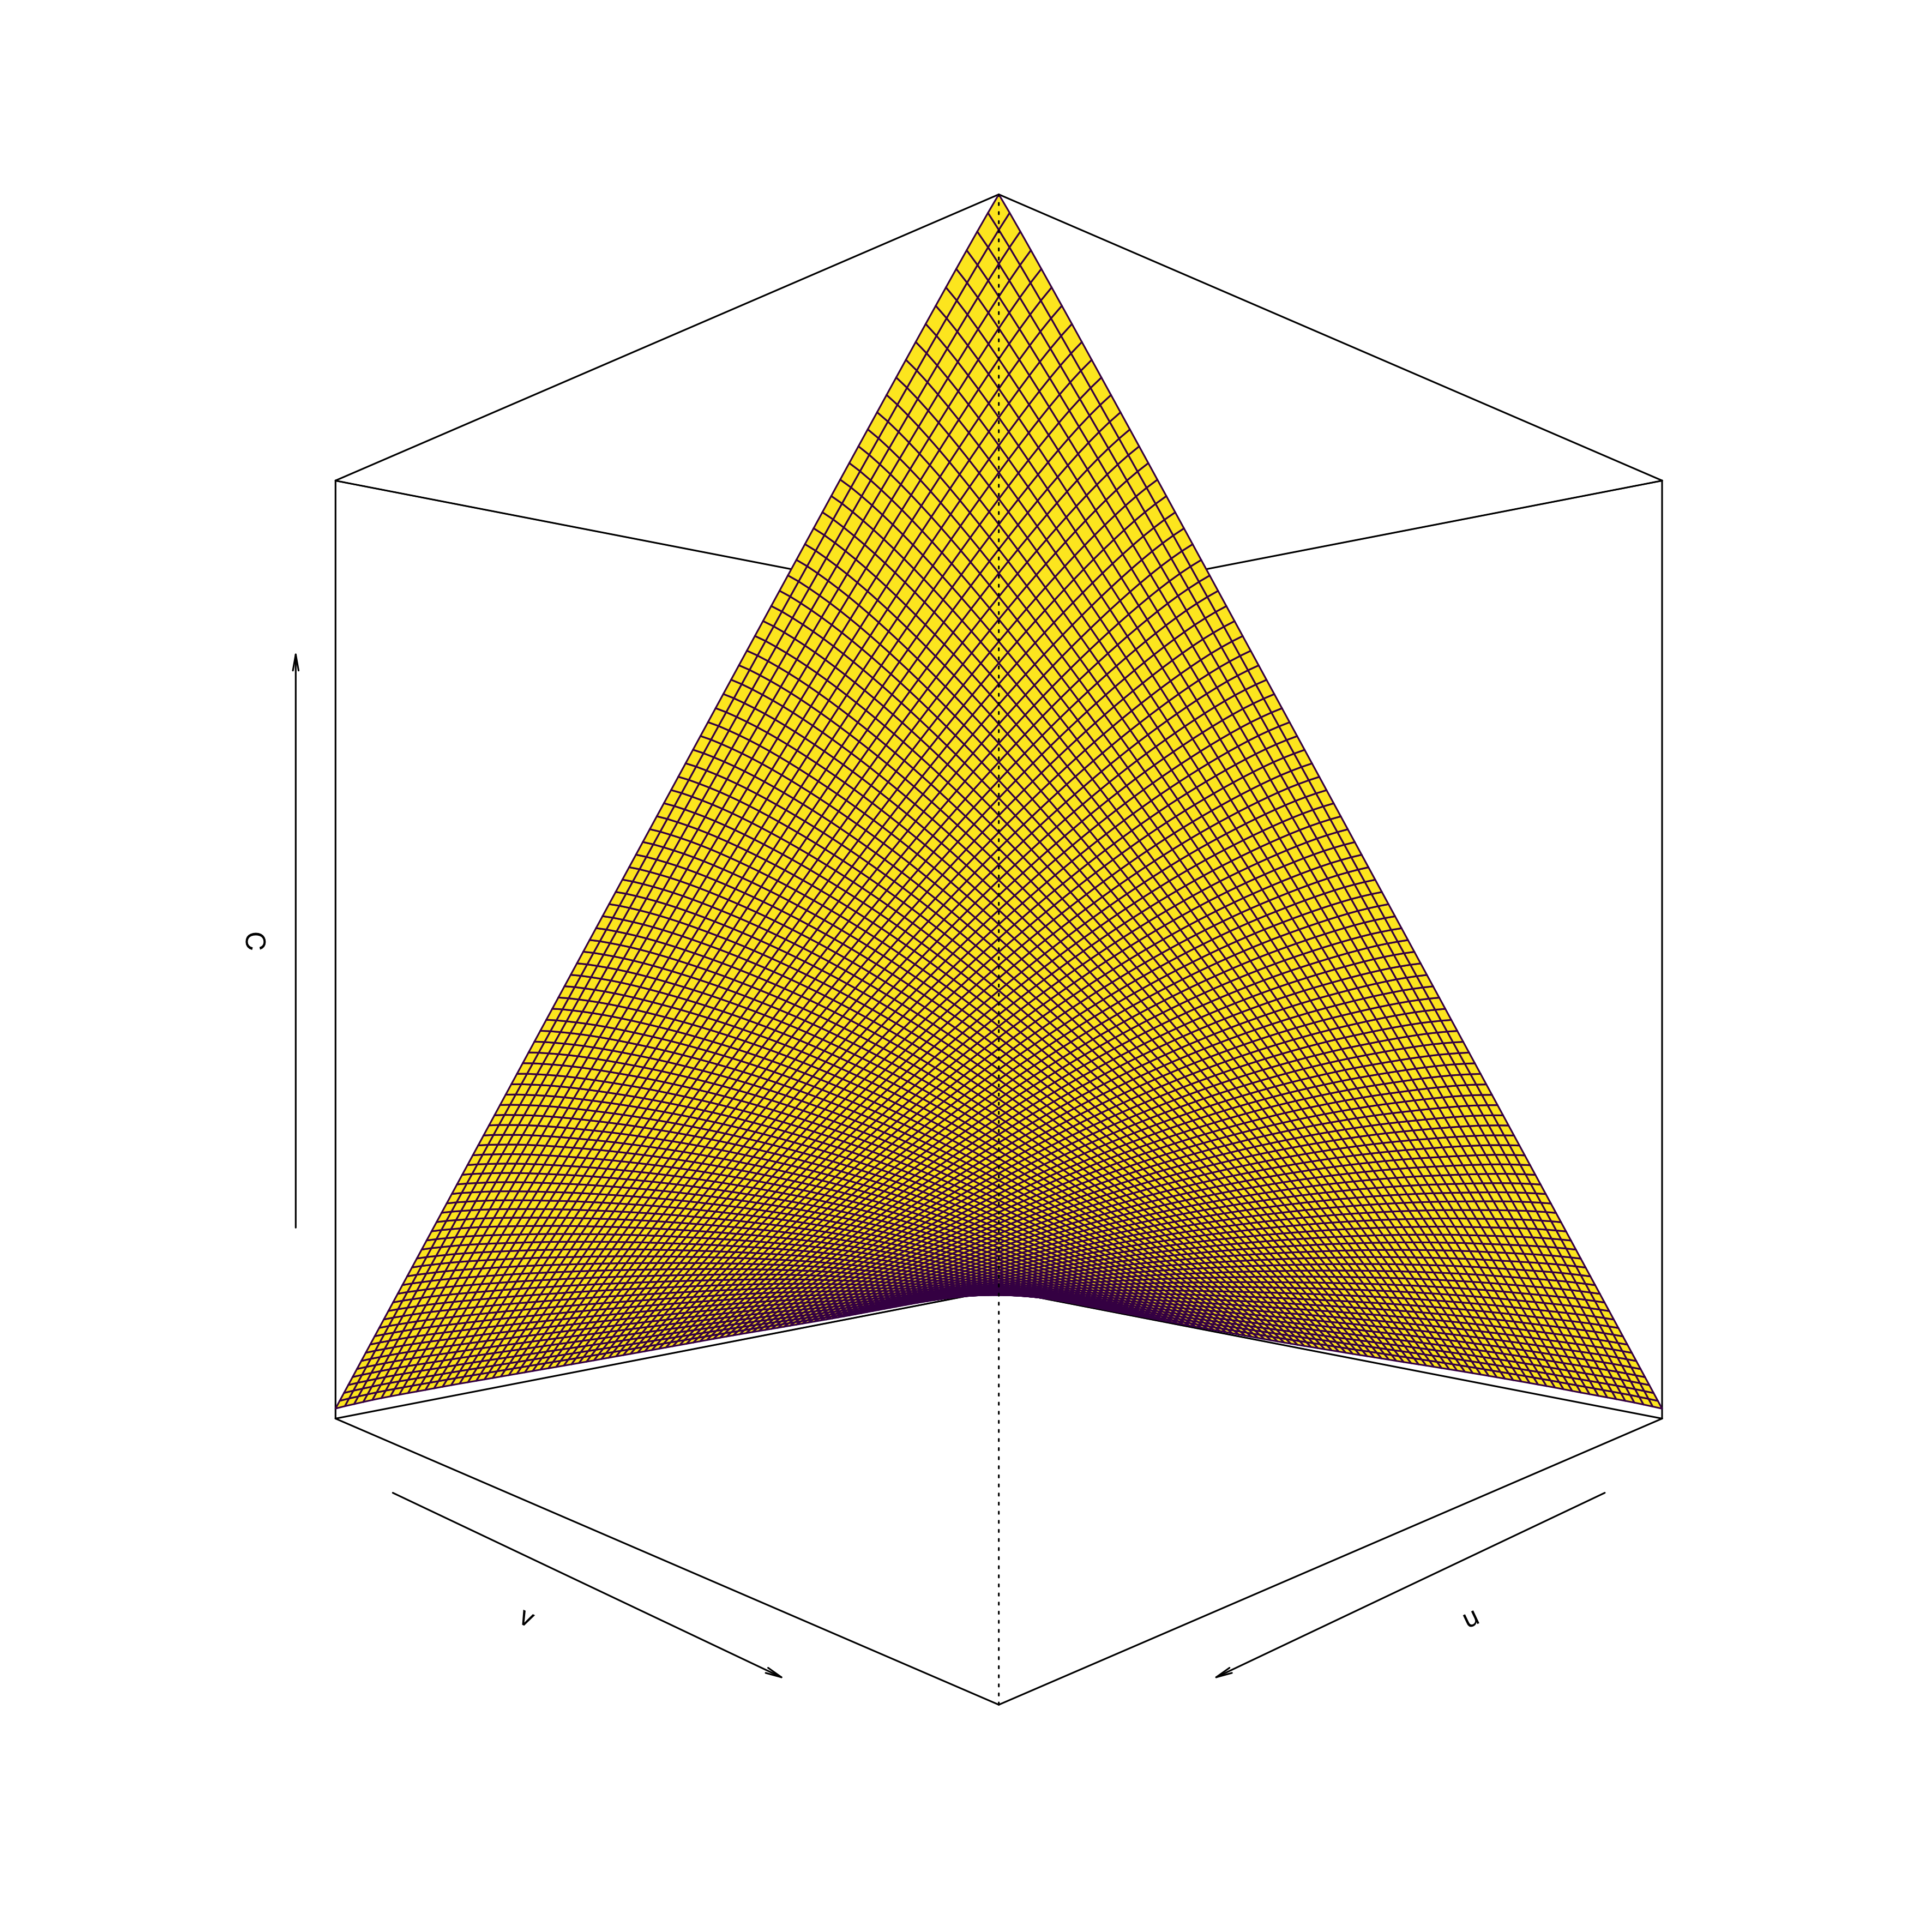
\includegraphics[width=10cm]{copula_5.png}
\caption{Gráfica de $\C (u, v)$ para $\gamma = 5$ en el cubo $(u, v, \C) \in [0, 1]^3$.}
\label{fig:copula}
\end{figure}

En la figura \ref{fig:copula}, se pueden notar gráficamente algunas de las propiedades de $\C$, como que cae a cero cuando $u \to 0$ o $v \to 0$ y que $\C (u, v) \to 1$ cuando $(u, v) \to (1, 1)$.\\

Ya que estudiamos las propiedades del modelo, pasamos a describir la distribución inicial de las tasas de riesgo $h_1$ y $h_2$, al igual que para el parámetro $\gamma$. En el siguiente apartado se calculan las distribuciones posteriores condicionales de todos los parámetros y se explica cómo simular observaciones de las distribuciones marginales utilizando el muestreador de Gibbs. También explicamos cómo incorporar las variables latentes $\omega_1$, $\omega_2$y $y$ en las simulaciones para poder obtener estimaciones muestrales de sus distribuciones.

\subsection{Distribuciones iniciales y posteriores}

Utilizando las ideas introducidas en su artículo \citet{old_nieto}, los autores definen una distribución inicial no paramétrica para las funciones de riesgo utilizando procesos de Markov de la siguiente manera.\\

Sea $(0 = \uptau_0 < \uptau_1 < \dots)$ una partición de la escala de tiempo  y $\lbrace u_k \rbrace$ un proceso latente. Entonces el proceso estacionario $\lbrace \lambda_k \rbrace$ se define tomando

\begin{enumerate}
\item $\lambda_1 \sim Ga(\alpha, \beta).$
\item $u_k | \lambda_k \sim Po(c_k\lambda_k).$
\item $\lambda_{k+1}|u_k \sim Ga(\alpha + u_k, \beta + c_k).$\\
\end{enumerate}

Así, la distribución inicial para $h_j(t)$ está dada por $$h_j(t) = \sum_k \lambda_{jk} \mathbb{I}\lbrace \uptau_{k-1} < t \leq \uptau_{k} \rbrace$$ y además se tiene que $$cor(\lambda_k, \lambda_{k+1}) = \frac{c_k}{c_k + \beta}.$$\\

Sea $\underline{T}_{(n)}$ una muestra de tamaño $n$ del vector aleatorio $T=(T_1, T_2)$ con función de densidad $f(t_1, t_2)$. Para simplificar la notación, omitimos la dependencia del parámetro $h = (h_1, h_2).$ La función de densidad conjunta de $T$ y el vector de variables latentes $\omega$ está dada por $$f(t_1, t_2, \omega_1, \omega_2) = f_1(t_1|\omega_1)f_2(t_2|\omega_2)m(\omega_1, \omega_2).$$\\

De la construcción \eqref{eq_omegas} tenemos que la distribución de $\omega$ depende de la variable latente $y$, por lo que, si asumimos independencia condicional de $\omega_1$ y $\omega_2$ dado $y$ podemos extender esta densidad conjunta para obtener
$$f(t_1, t_2, \omega_1, \omega_2, y)= f_1(t_1|\omega_1)f_2(t_2|\omega_2)m(\omega_1|y)m(\omega_2|y)g(y).$$\\

Nos interesa obtener la distribución posterior de las funciones de riesgo $h_1$ y $h_2$. Para obtenerlas debemos calcular $$p(h | t) = \int_{\Omega} \int_{S_Y} p(h | t, \omega, y) \ dy \ d\omega.$$ Sin embargo, podemos evitar la marginalización sobre $\omega$ y $y$ trabajando como si estas dos variables fueran observadas junto con $T$. Así, cada observación $(t_{i1}, t_{i2})$ del vector $T$ necesita del vector de variables latentes $(\omega_{i1}, \omega_{i2}, y_i)$. Si la muestra consiste únicamente de observaciones exactas, la función de verosimilitud está dada por 
$$\mathcal{L}(t, \omega, y | h) = \prod_{i=1}^n f_1(t_{i1}|\omega_{i1})f_2(t_{i2}|\omega_{i2})m(\omega_{i1}|y_i)m(\omega_{i2}|y_i)g(y_i)$$\\

Utilizamos el Teorema de Bayes para obtener la distribución posterior de $h$, la cual es proporcional al producto de la verosimilitud y la distribución inicial $$\pi(h | t, \omega, y) \propto \mathcal{L}(t, \omega, y | h) \pi(h).$$ Recordemos que la distribución inicial de $h$ depende de los procesos $\lbrace \lambda_j \rbrace$ y $\lbrace u_j \rbrace$ $(j = 1, 2)$.\\

Recordemos que las variables $\omega$ y $y$ no son observadas. Entonces, para simular observaciones de la distribución posterior de $h$ utilizando el muestreador de Gibbs, necesitamos expresiones para las distribuciones posteriores condicionales de $\omega, y, \lambda$ y $u$ que calculamos a continuación.

\subsubsection{$\omega_{ij}$}
\label{posterior_omega}

La distribución posterior de $\omega_{ij}$ es de la forma

\begin{align*}
m(\omega_{ij} | t, y, h) &\propto p(t, y, h, \omega)\\
&\propto \mathcal{L}(t, \omega, y |h) \pi(h)\\
&\propto \mathcal{L}(t, \omega, y |h)\\
&\propto f_j(t_{ij}|\omega_{ij})m(\omega_{ij}|y_i)\\
&\propto \frac{h_j(t_{ij})}{\omega_{ij}}\mathbb{I}\lbrace \omega_{ij} > H_j(t_{ij})\rbrace \  \omega_{ij}^{1+y_i} \ \exp (-(1+\gamma)\omega_{ij})\\
&\propto \omega_{ij}^{y_i} \ e^{-(1+\gamma)\omega_{ij}} \ \mathbb{I}\lbrace \omega_{ij} > H_j(t_{ij})\rbrace.\\
\end{align*}

La forma funcional se asemeja a una distribución Gamma, pero la restricción sobre el dominio de $\omega_{ij}$ altera esta distribución. Para obtener una simulación de esta distribución en el paso $(t+1)$ se utiliza el algoritmo de Metropolis-Hastings.\\

Como distribución candidata se analizaron dos opciones. Primero, se utilizó una distribución gamma trasladada, independiente de $\omega_{ij}^{(t)}$, de la forma $$f_1 \sim Ga(1 + y_i^{(t)}, 1 + \gamma^{(t)}) + H_j(t_{ij})^{(t)}.$$ La segunda opción fue una distribución uniforme de la forma $$f_2 \sim U(\max \lbrace H_j(t_{ij})^{(t)}, \ \omega_{ij}^{(t)} - a \rbrace, \ \omega_{ij}^{(t)} + a),$$ donde $a$ es una constante positiva.\\

Realizando algunos experimentos con ambas opciones, se utilizó finalmente la distribución uniforme. Esto se debe a que las propuestas independientes de la gamma trasladada tienden a rechazar más propuestas que la distribución uniforme y la cadena se ``atora" más. Como ejemplo se incluye la simulación de una cadena con cada propuesta, para los valores fijos $a = 3$, $\gamma = 1$ y $H_j(t_{ij}) = 0.9$.\\

\begin{figure}[H] 
\centering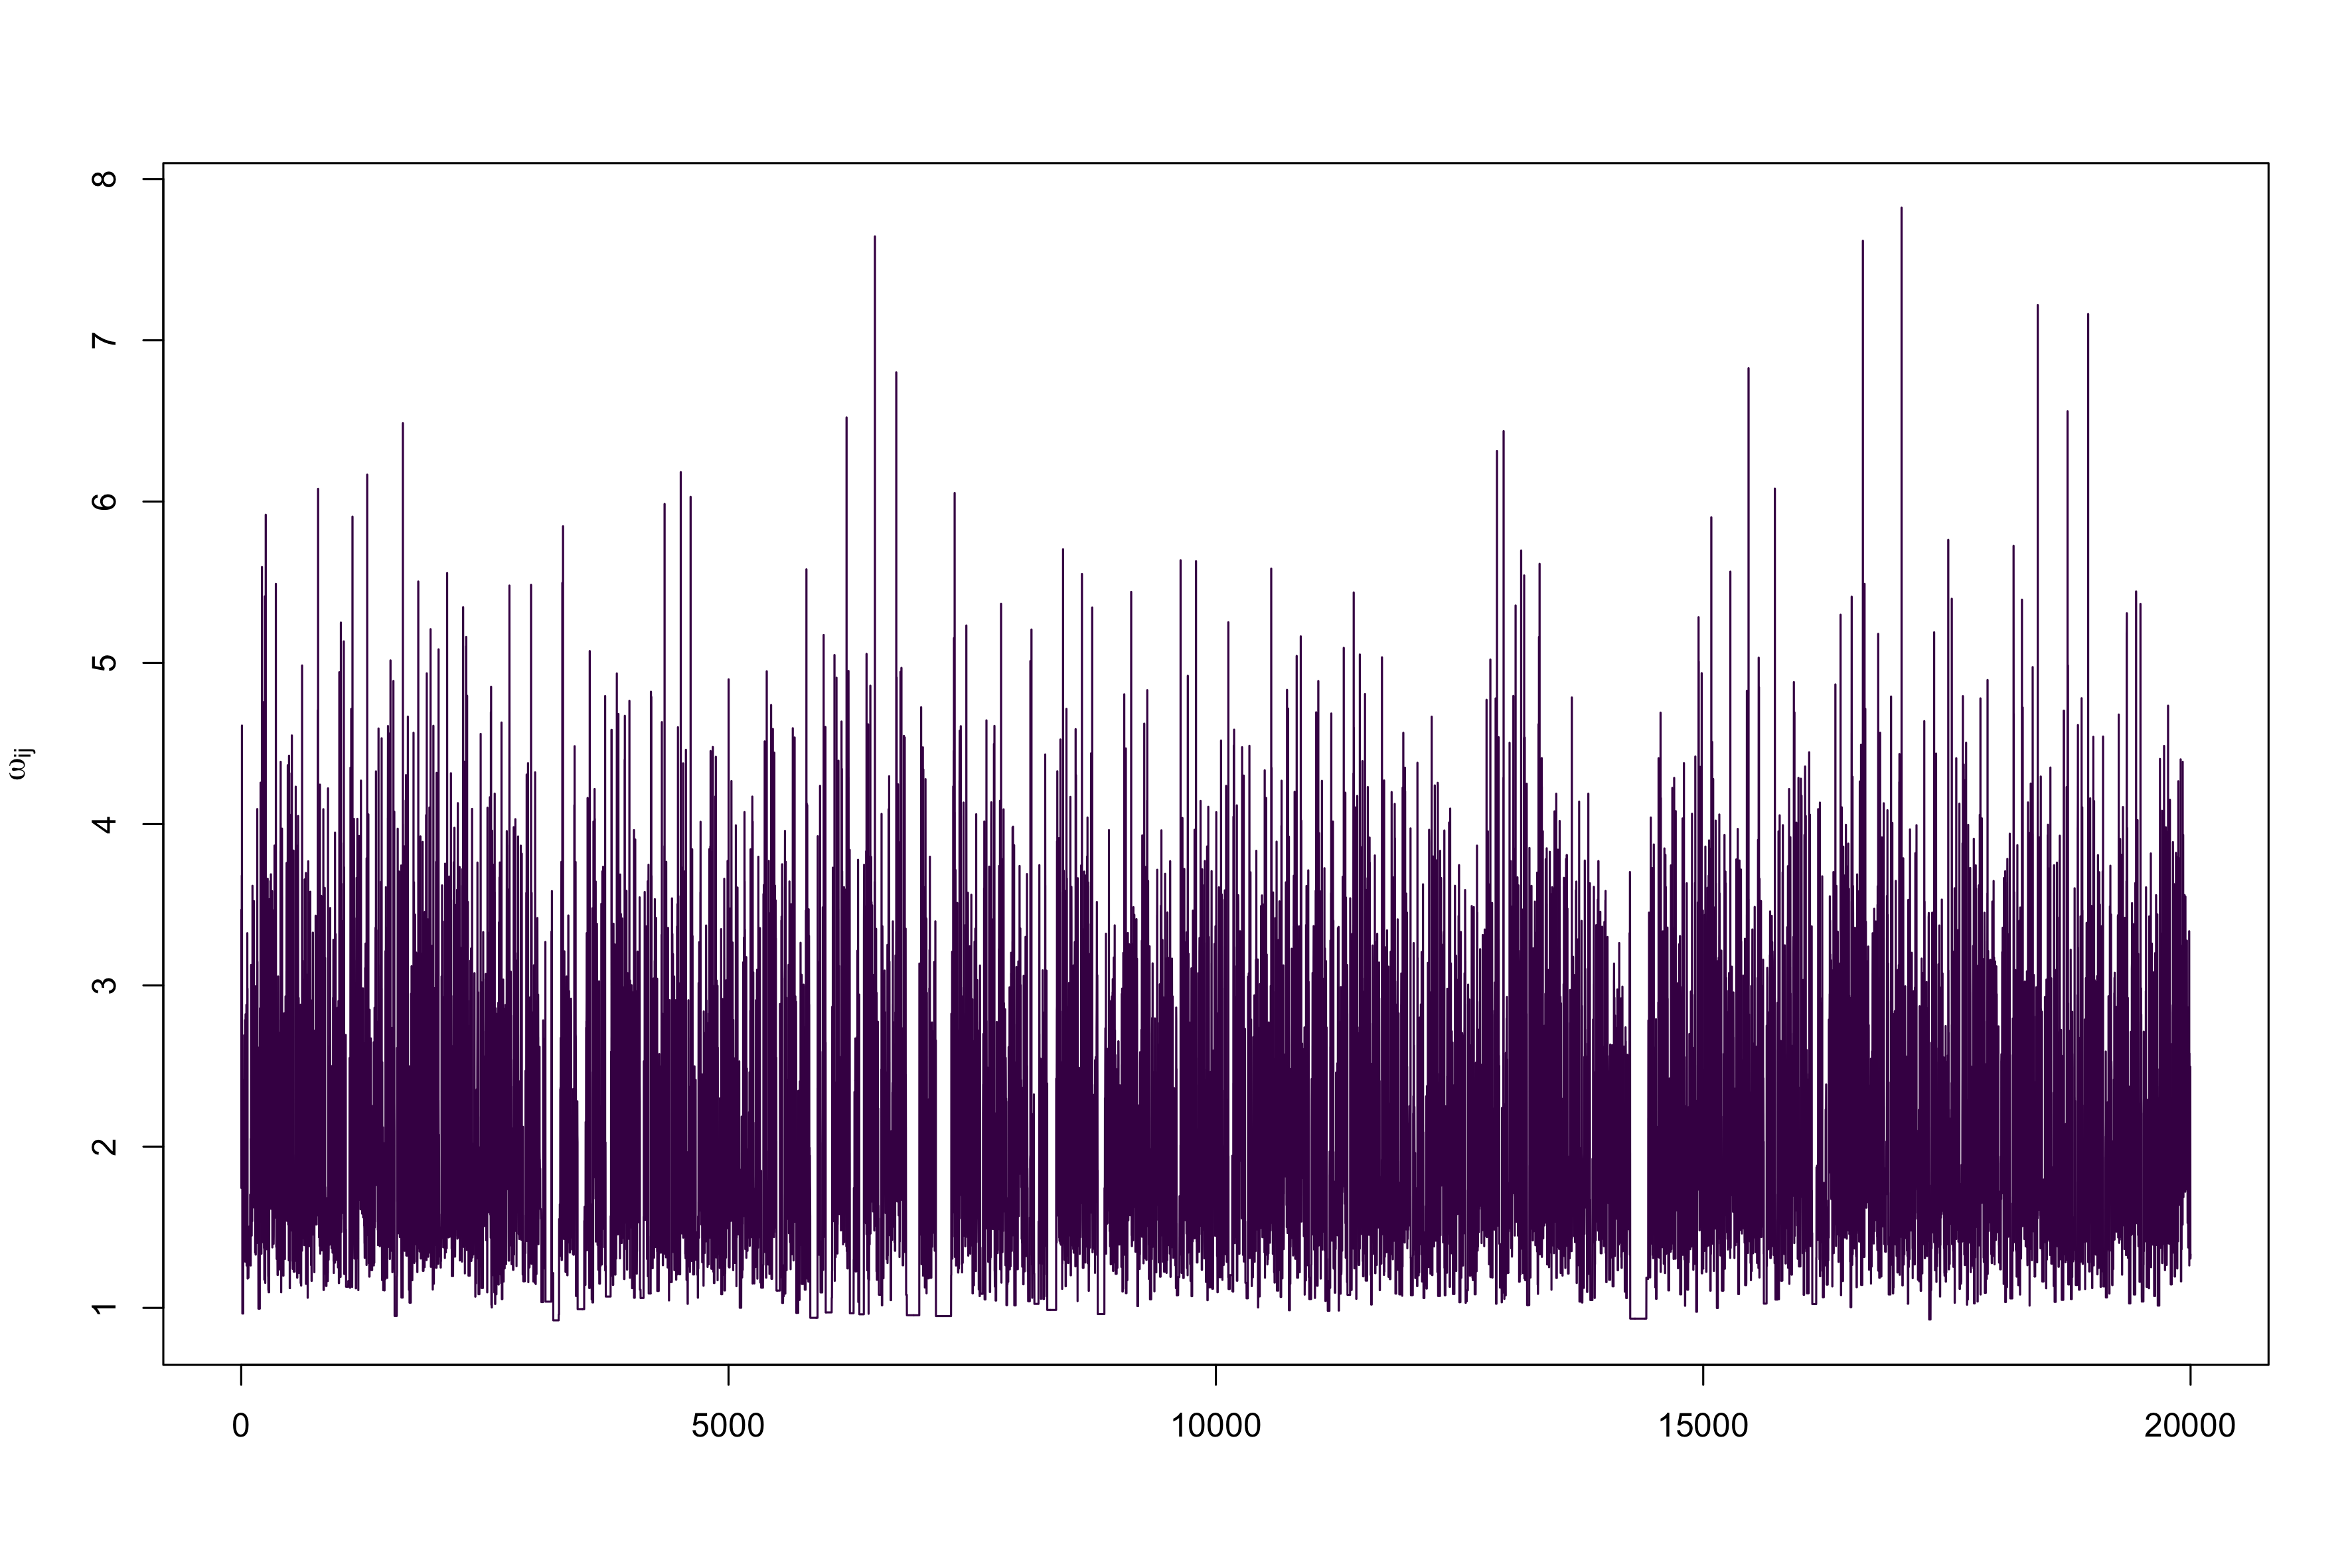
\includegraphics[width=10cm]{propuesta_gamma.png}
\caption{Cadena de Markov para $\omega_{ij}$ con propuestas $f_1$.}
\label{fig:prop_gamma}
\end{figure}

\begin{figure}[H] 
\centering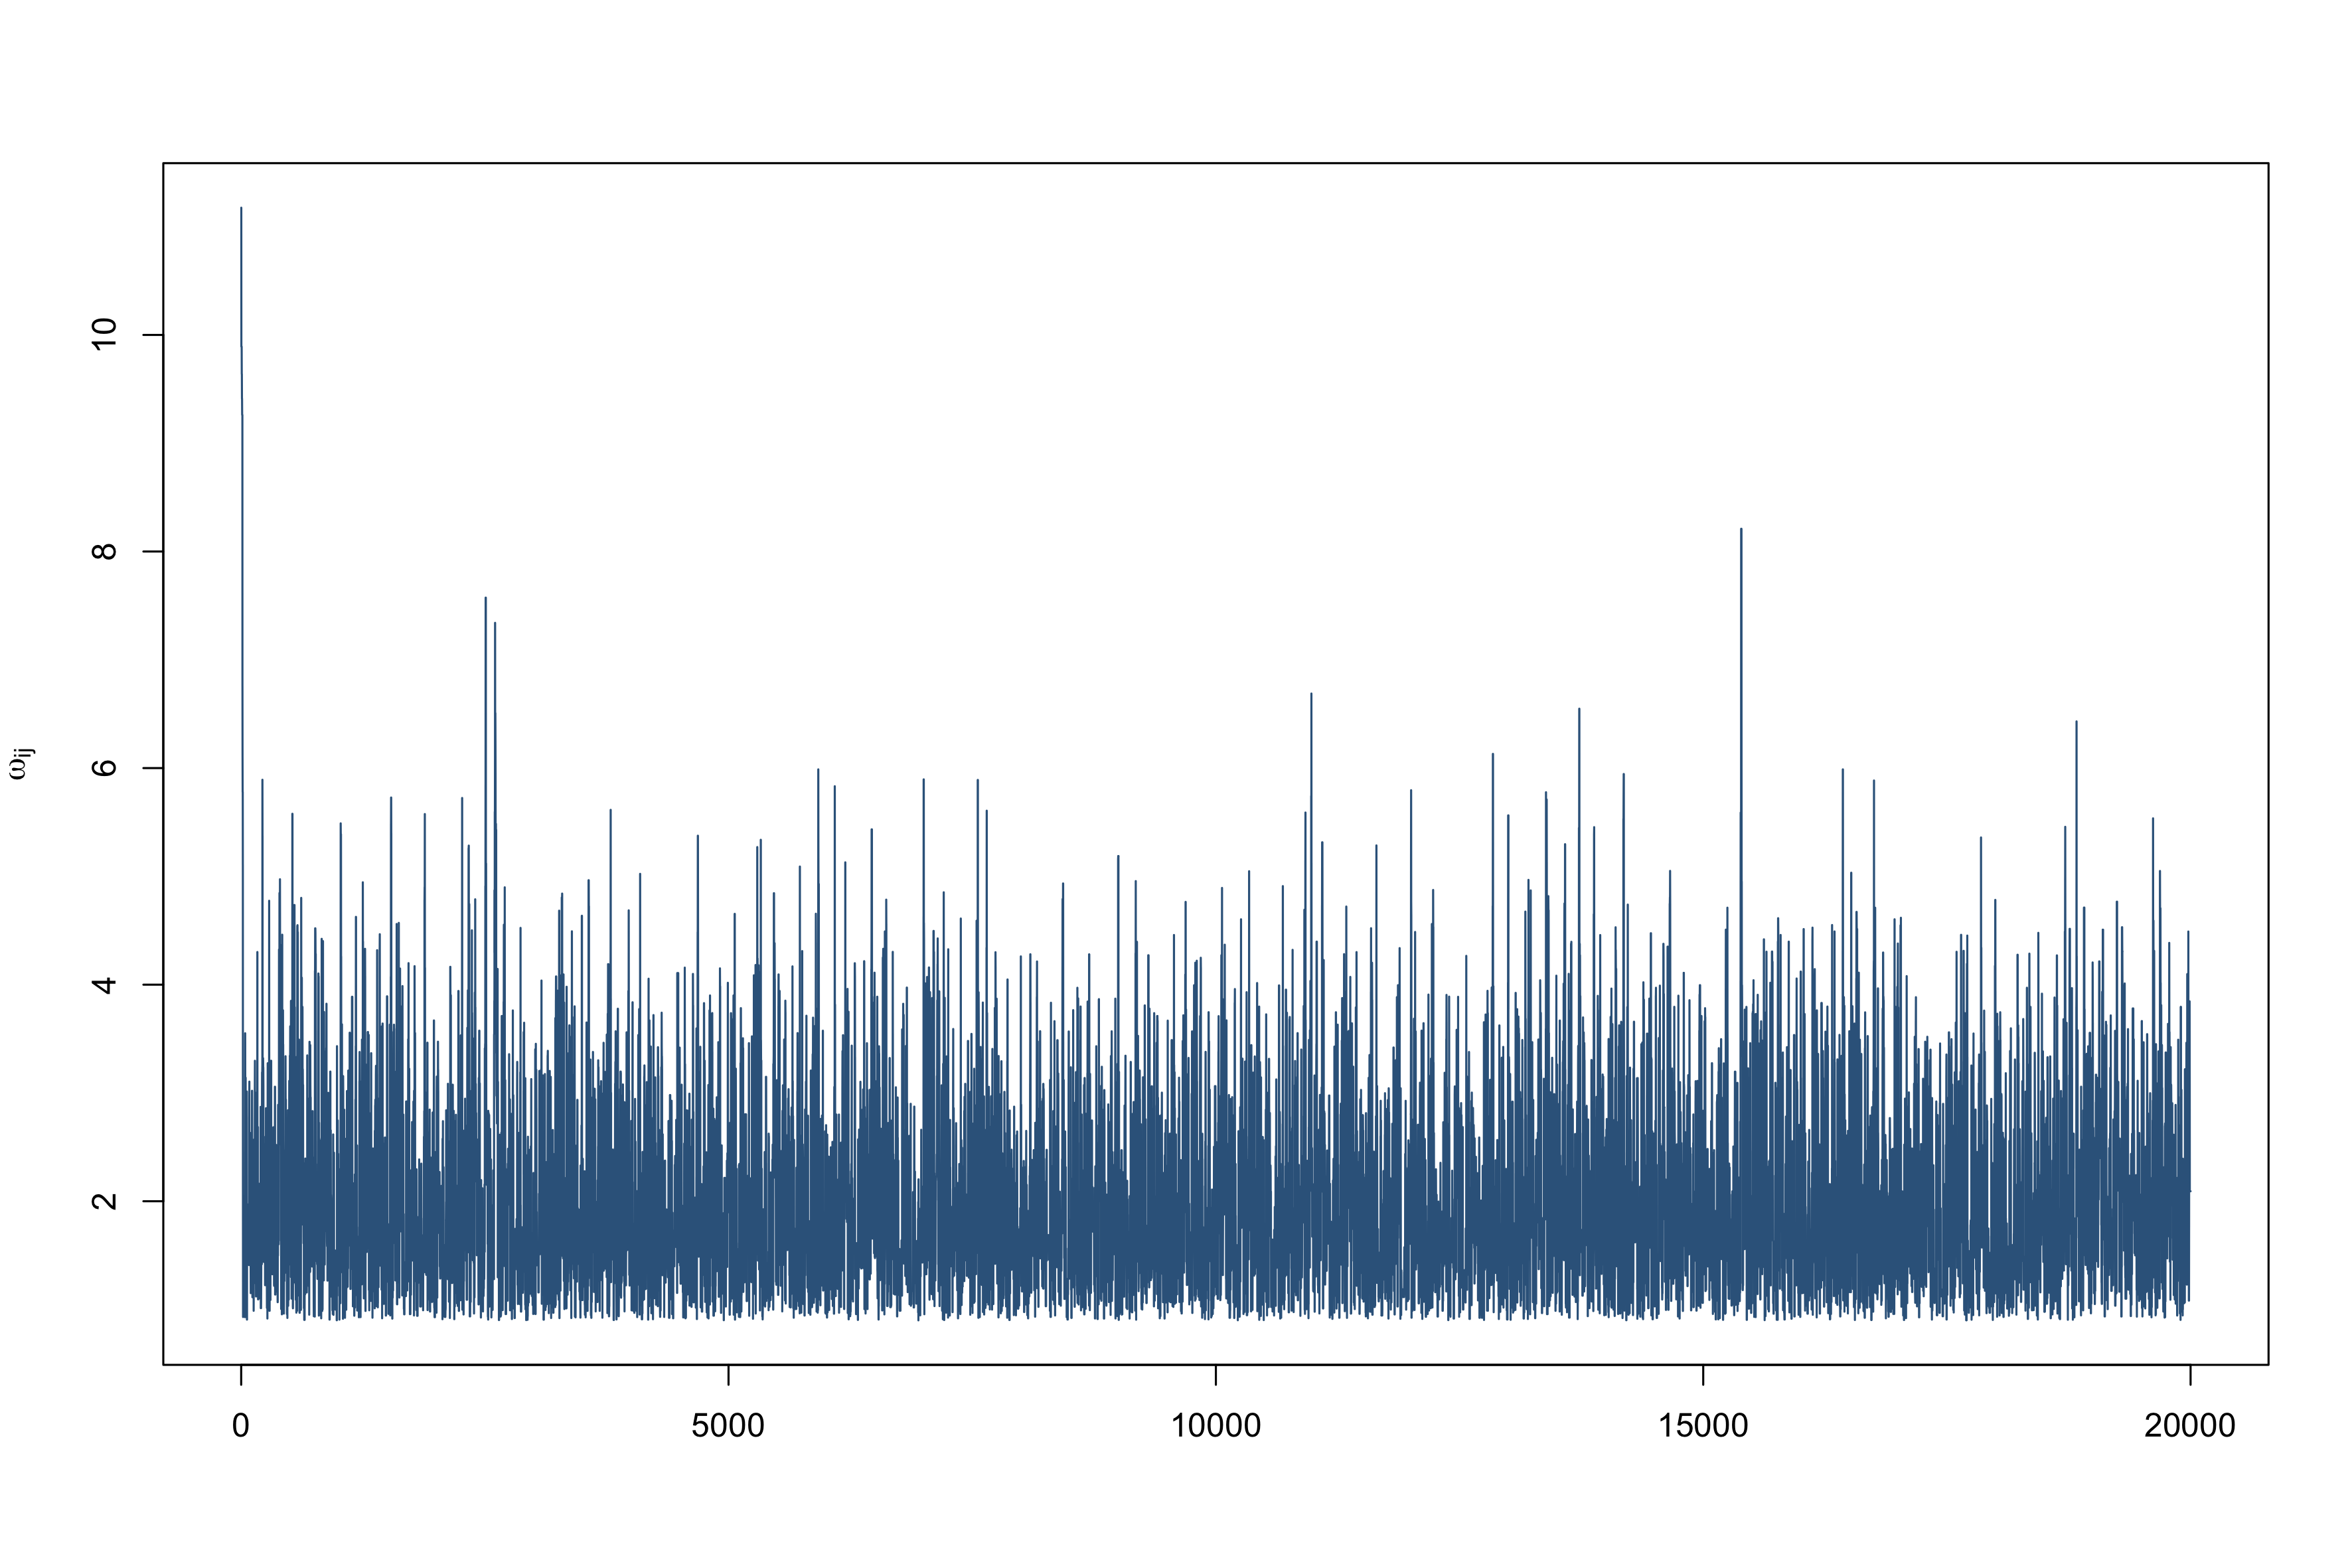
\includegraphics[width=10cm]{propuesta_uniforme.png}
\caption{Cadena de Markov para $\omega_{ij}$ con propuestas $f_2$.}
\label{fig:prop_unif}
\end{figure}

Podemos ver que la figura \ref{fig:prop_unif} tiene menos espacios en blanco, que son pedazos en donde la cadena se atora. Además, parece que con las propuestas uniformes la cadena explora más valores del soporte que con las propuestas gamma independientes.\\

Para programar el paso de Metropolis-Hastings debemos calcular la razón de Hastings. Denotemos $\omega^*$ a la observación candidata. Como las propuestas vienen de una distribución uniforme, el cociente de la densidad candidata $f_2(\omega_{ij} ^{(t)} | \omega^*)/f_2(\omega^* | \omega_{ij} ^{(t)})$ siempre es igual a 1, por lo que no es necesario incorporarlo. Entonces el logaritmo de la razón de Hastings queda de la siguiente forma:

\begin{align*}
\log (r(\omega_{ij}^{(t)}, \omega^*)) &= \log \left(\frac{m(\omega^* | y_i, \gamma)}{m(\omega_{ij}^{(t)}| y_i, \gamma)}\right)\\
&= y_i \left(\log (\omega^*) - \log (\omega_{ij}^{(t)}\right) - (1 + \gamma)(\omega^* - \omega_{ij}^{(t)}).
\end{align*}

Así, el código para simular una observación del vector $\omega_j$ es como sigue.\\

\begin{lstlisting}
  sample_omega <- function(omega, y, cum_h, x, theta, gamma, omega_d = NULL) {

  if (is.null(omega_d)) omega_d <- y + 1

  bound <- cum_h * exp(x %*% theta)
  l1 <- max(bound, omega - omega_d)
  l2 <- omega + omega_d
  proposal <- stats::runif(n = 1, min = min(l1, l2), max = max(l1, l2))

  if (omega <= bound) {
    omega_out <- proposal
    return(omega_out)
  }

  log_alpha <-
    y * (log(proposal) - log(omega)) - (1 + gamma) * (proposal - omega)
  prob <- min(exp(log_alpha), 1)
  u <- stats::runif(n = 1)
  omega_out <- omega + (proposal - omega) * (u <= prob)

}
\end{lstlisting}


\subsubsection{$y_i$}
\label{posterior_y}

La distribución posterior de $y_i$ es proporcional a

\begin{align*}
g(y_i | t, \omega, h) &\propto p(t, y, h, \omega)\\
&\propto \mathcal{L}(t, \omega, y |h) \pi(h)\\
&\propto \mathcal{L}(t, \omega, y |h)\\
&\propto m(\omega_{i1}|y_i)m(\omega_{i2}|y_i)g(y_i)\\
&\propto \frac{\left[\gamma (1+\gamma) \ \omega_{i1} \ \omega_{i2}\right]^{y_i}}{\Gamma(2+y_i)\Gamma(1+y_i)}.
\end{align*}

Recordemos que $y_i$ es una variable latente discreta, por lo que para aproximar la constante de la función de probabilidad utilizamos la técnica de la sección \ref{sec:transformada}. Una vez que se aproxime esta constante, se puede aproximar la función de distribución y obtenemos una muestra de $y_i^{(t+1)}$ con el método de la transformación inversa.\\

El código se divide en dos partes. Primero aproximamos la constante y creamos la función de distribución $G(y_i) = P(Y_i \leq y_i)$. Debemos agregar verificaciones de estabilidad, ya que las funciones $\Gamma$ pueden tomar valores muy grandes que son tomados como infinitos por R. También por estabilidad numérica trabajamos con el logaritmo de la función de probabilidad.\\

\begin{lstlisting}
log_density_y <- function(y, omega1, omega2, gamma) {

  y * (log(gamma) + log(1 + gamma) + log(omega1) + log(omega2)) -
    lgamma(1 + y) - lgamma(2 + y)

}
\end{lstlisting}

\begin{lstlisting}
prob_y <- function(omega1, omega2, gamma) {

  y <- vector(mode = "numeric", length = 5e2)
  acum <- 0
  j <- 0
  prob <- 1

  while (j <= 5e2 & prob > 1e-6) {
    gj <- exp(log_density_y(j, omega1, omega2, gamma))
    if (is.nan(gj)) {
      break
    }
    prueba_acum <- acum + gj
    if (is.infinite(prueba_acum)) {
      break
    }
    if (prueba_acum == 0) {
      break
    }
    acum <- prueba_acum
    prob <- gj / acum
    y[j + 1] <- gj
    j <- j + 1
  }

  y <- y[1:j] / acum
  prob_fun <- cumsum(y)

}
\end{lstlisting}

Este código genera la función de distribución, que luego utilizamos para obtener las observaciones con la inversa generalizada como sigue.\\

\begin{lstlisting}
 sample_y <- function(omega1, omega2, gamma) {

  distribution <- prob_y(omega1, omega2, gamma)

  if(is.na(distribution[1])) {
    distribution <- c(1)
    warning("No distribution for Y")
  }

  u <- stats::runif(n = 1)
  index <- 1

  while (u > distribution[index]) {
    index <- index + 1
  }

  y <- index - 1

}
\end{lstlisting}

Estos códigos los implementamos en forma de funciones para poderlas llamar fácilmente en cada iteración del muestreador de Gibbs. Ahora obtenemos la distribución posterior de $\lambda_{jk}$ y explicamos cómo obtener muestras de ella.

\subsubsection{$\lambda_{jk}$}
\label{posterior_lambda}

Obtengamos la forma de la posterior para este parámetro.\\

\begin{align*}
\pi(\lambda_{jk} | t, \omega, y, u, \lambda_{-jk}) &\propto \pi(\lambda, t, \omega, y, u)\\
&\propto \mathcal{L}(t, \omega, y | \lambda, u) \pi(\lambda, u).
\end{align*}

Por un lado tenemos
\begin{align} \label{lambda_ver}
\mathcal{L}(t, \omega, y | \lambda, u) &\propto \prod_{i = 1}^n h_j(t_{ij}) \mathbb{I}\lbrace \omega_{ij} > H_j(t_{ij}) \rbrace \nonumber\\
&\propto \lambda_{jk}^{n_{jk}} \prod_{i = 1}^n \mathbb{I}\lbrace \omega_{ij} > H_j(t_{ij}) \rbrace
\end{align}

donde $$n_{jk} = \sum_{i=1}^n \mathbb{I}(\uptau_{k-1} < t_{ij} \leq \uptau_k)$$ y $$H_j(t) = \sum_{m = 1}^{k-1} \lambda_{jm}(\uptau_m - \uptau_{m-1}) + \lambda_{jk}(t - \uptau_{k-1})$$ para $t\in (\uptau_{k-1}, \uptau_k].$\\

Por otro lado, recordando que $$u_{jk}|\lambda_{jk} \sim Po(c_{jk}\lambda_{jk})$$ y $$\lambda_{jk}|u_{j,k-1} \sim Ga(\alpha + u_{j, k-1}, \beta + c_{k-1}),$$ tenemos
\begin{align} \label{lambda_prior}
\pi(\lambda, u) &\propto \pi(u_{jk} | \lambda, u_{-jk})\pi(\lambda, u_{-jk}) \nonumber \\
&\propto \pi(u_{jk} | \lambda_{jk})\pi(\lambda_{jk}| u_{j, k-1}) \nonumber \\
&\propto \lambda_{jk}^{u_{jk} + u_{j, k-1} + \alpha - 1} \ \exp\lbrace-\lambda_{jk}(c_{jk} + c_{j, k-1} + \beta)\rbrace. \nonumber \\
\end{align}

Así, juntando \eqref{lambda_ver} y \eqref{lambda_prior}, tenemos que
\begin{equation*}
\pi(\lambda_{jk} | t, \omega, y, u, \lambda_{-jk}) \propto \lambda_{jk}^{n_{jk} + u_{jk} + u_{j, k-1} + \alpha - 1} \ e^{-\lambda_{jk}(c_{jk} + c_{j, k-1} + \beta)} \prod_{i=1}^n \mathbb{I}\lbrace \omega_{ij} > H_j(t_{ij}) \rbrace.\\
\end{equation*}

El producto $\prod_{i=1}^n \mathbb{I}\lbrace \omega_{ij} > H_j(t_{ij}) \rbrace$ impone una restricción sobre el dominio de $\lambda_{jk}$ de la forma $\lambda_{jk} < b_{jk}$, por lo que la distribución de $\lambda_{jk}$ es una gamma truncada.\\

Para poder obtener una muestra de esta distribución en cada paso del muestreador de Gibbs, debemos realizar dos pasos:
\begin{enumerate}
\item Actualizar la cota $b_{jk}.$
\item Obtener una muestra de la gamma truncada.\\
\end{enumerate}

Para realizar el primer paso, veamos qué tipo de restricciones puede poner $\omega_{ij} > H_j(t_{ij})$ sobre $\lambda_{jk}$. Veamos el caso de $\lambda_{j1}$. Si $t_{1j} \in (\tau_0, \tau_1]$, entonces tenemos que $H_j(t_{1j}) = \lambda_{j1}(t_{1j} - \tau_0)$ y la restricción es de la forma $\lambda_{j1} < \omega_{1j} / (t_{1j} - \tau_0)$.\\

Por otro lado, si $t_{1j} \in (\tau_1, \tau_2]$, entonces $H_j(t_{1j}) = \lambda_{j1}(\tau_1 - \tau_0) + \lambda_{2j}(t_{1j} - \tau_1)$ y la restricción es de la forma $$\lambda_{j1} < \frac{\omega_{1j}-\lambda_{j2}(t_{1j} - \tau_1)}{\tau_1 - \tau_0}.$$\\

Si nos fijamos ahora en $\lambda_{j2}$, podemos ver que cualquier $t_{ij} \in (\tau_0, \tau_1]$ no impone restricciones sobre su dominio. En resumen, el tipo de restricciones que impone $\omega_{ij} > H_j(t_{ij})$ sobre $\lambda_{jk}$ depende de si $t_{ij}$ se encuentra en el intervalo de $\lambda_{jk}$ o en uno posterior.\\

Ya que conocemos la cota, falta ver cómo obtenemos muestras de la gamma truncada. Denotemos $\lambda^*$ al límite superior del soporte de $\lambda_{jk}$. Usaremos el hecho de que si $X \sim Ga(\alpha, 1)$, entonces $Y = X/\beta \sim Ga(\alpha, \beta)$. Sea $F$ la función de distribución de $X$ y $G$ la función de distribución de $Y$. Tenemos que
\begin{align*}
F(x) &= P\lbrace X \leq x\rbrace\\
&= P\lbrace \beta Y \leq x \rbrace\\
&= P\lbrace Y \leq x/\beta \rbrace\\
&= G(x/\beta).\\
\end{align*}

Por lo tanto, se tiene que $F(\lambda^* \beta) = G(\lambda^*)$. Si queremos truncar el soporte de $Y$ a $(0, \lambda^*)$ necesitamos reescalar la distribución. Si $Y'$ es la variable aleatoria truncada y $G'$ su función de distribución, entonces se tiene que $G'(y) = \frac{1}{G(\lambda^*)} G(y)$ para $y \in S_{Y'}$. Finalmente, para utilizar el método de la transformación inversa, simulamos $u\sim U(0, 1)$ y buscamos $x$ tal que
\begin{align*}
F(x) / F(\beta \lambda^*) &= u \implies\\
F(x) / G(\lambda^*) &= u \implies\\
G(x/\beta) / G(\lambda^*) &= u \implies\\
G'(x/\beta) = u\\
\end{align*}
y de aquí concluimos que una observación de la posterior de $\lambda_{jk}$ se obtiene con $\lambda_{jk} = x/\beta$.\\

Ahora se presenta el código en R para realizar estas simulaciones. Primero, buscamos la cota para $\lambda_{jk}$. Se utilizan las funciones auxiliares \texttt{partition\_location} y \texttt{partition\_count}. La primera nos dice en que intervalo de la partición de tiempos se encuentra cada observación, mientras que la segunda nos dice cuántas observaciones hay en cada intervalo. El código para estas funciones se encuentra en el apéndice \ref{ap:partition_functions}.\\

\begin{lstlisting}
lambda_restriction <- function(t,
                               omega,
                               x,
                               part_loc,
                               t_partition_low,
                               lambda_index,
                               theta,
                               lambda,
                               part_len) {

  omega_h <- omega * exp(-(x %*% theta))

  if (lambda_index < part_loc) {
    current_bound <- 0

    if (part_loc > 1) {
      for (k in 1:(part_loc - 1)) {
        current_bound <-
          current_bound + (lambda[k] * part_len) * (k != lambda_index)
      }
    }

    current_bound <-
      current_bound + lambda[part_loc] * (t - t_partition_low)
    current_bound <- (omega_h - current_bound) / part_len

    if (is.na(current_bound)) {
      warning("Lambda bound failed")
      current_bound <- 2
    }

  } else if (lambda_index == part_loc) {
    current_bound <- 0

    if (part_loc > 1) {
      for (k in 1:(part_loc - 1)) {
        current_bound <- current_bound + (lambda[k] * part_len)
      }
    }

    current_bound <- (omega_h - current_bound) / (t - t_partition_low)

    if (is.na(current_bound)) {
      warning("Lambda bound failed")
      current_bound <- 2
    }

  } else {

    current_bound <- 2

  }

  return(current_bound)

}
\end{lstlisting}

Ya que se tiene la cota, podemos proceder a realizar la simulación. Para resolver la ecuación de la forma $f(x) - u = 0$ se utiliza la función \texttt{uniroot} del paquete \texttt{stats} que viene con la instalación básica de R.\\

\begin{lstlisting}
sample_lambda <- function(u1, u2, alpha, beta, c1, c2, min_bound, part_count) {

  # u2 = 0 if lambda is the first interval
  # c2 = c1 if lambda is not in the first interval
  alpha_l <- alpha + u1 + u2 + part_count
  beta_l <- beta + c1 + c2

  if (min_bound < 1e-6) min_bound <- 1
  denominator <- stats::pgamma(min_bound * beta_l, shape = alpha_l, rate = 1)
  if (denominator == 0) denominator <- 0.005
  unif <- stats::runif(n = 1)

  f <- function(x) {
    stats::pgamma(x, shape = alpha_l, rate = 1) / denominator - unif
  }

  solution <- stats::uniroot(f, lower = 0, upper = min_bound * beta_l)$root
  lambda_prueba <- solution / beta_l
  if (lambda_prueba < 1e-5) lambda_prueba <- 1e-5
  lambda <- lambda_prueba

}
\end{lstlisting}



\subsubsection{$u_{jk}$}

La posterior para este parámetro es de la siguiente forma.\\

\begin{align*}
\pi(u_{jk} | t, \omega, y ,\lambda) &\propto \mathcal{L}(t, \omega, y | u, \lambda) \pi(u, \lambda)\\
&\propto \pi(u, \lambda)\\
&\propto \pi(\lambda_{j, k+1} | u, \lambda_{-(j, k+1)}) \pi(u, \lambda_{-(j, k+1)})\\
&\propto \pi(\lambda_{j, k+1} | u_{jk}) \pi(u_{jk}|\lambda{jk})\\
&\propto \frac{(\beta + c_{jk})^{\alpha + u_{jk}}}{\Gamma(\alpha + u_{jk})} \left(\lambda_{j, k+1}^{\alpha + u_{jk}-1}\right) \ \frac{\left(c_{jk}\lambda_{jk}^{u_{jk}}\right)}{\Gamma(u_{jk}+1)}\\
&\propto \frac{\left[c_{jk}\lambda_{jk}\lambda_{j, k+1}(\beta + c_{jk})\right]^{u_{jk}}}{\Gamma(\alpha + u_{jk})\Gamma(1 + u_{jk})}.\\
\end{align*}

Como el dominio de $u_{jk}$ es $\mathbb{N}\cup \lbrace 0 \rbrace$, utilizamos la misma técnica de simulación que para $y_i$. Esto es, aproximamos la constante de la distribución para construir la función de distribución y después utilizamos el método de la transformación inversa. No ahondaremos más en este algoritmo, ya que es muy similar al mencionado anteriormente. El código se incluye a continuación.\\

\begin{lstlisting}
prob_u <- function(l, l1, alpha, beta, c, index) {

  u <- vector(mode = "numeric", length = 5e2L)
  acum <- 0
  j <- 0
  prob <- 1

  while (j <= 5e2 & prob > 1e-6) {
    pi_j <- exp(log_density_u(j, l, l1, alpha, beta, c, index))
    if (is.nan(pi_j)) {
      break
      }
    prueba_acum <- acum + pi_j
    if (is.infinite(prueba_acum)) {
      break
      }
    if (prueba_acum == 0) {
      break
      }
    acum <- prueba_acum
    prob <- pi_j / acum
    u[j + 1] <- pi_j
    j <- j + 1
  }

  u <- u[1:j] / acum
  prob_fun <- cumsum(u)

}
\end{lstlisting}

\begin{lstlisting}
sample_u <- function(l, l1, alpha, beta, c, index_indicator) {

  distribution <- prob_u(l, l1, alpha, beta, c, index_indicator)

  if(is.na(distribution[1])) {
    distribution <- c(1)
    warning("No distribution for U")
  }

  u <- stats::runif(n = 1)
  index <- 1

  while (u > distribution[index]) {
    index <- index + 1
  }

  y <- index - 1

}
\end{lstlisting}

\subsubsection{El parámetro $\gamma$}

Recordemos de la sección \ref{caso_bivariado} que la dependencia entre las componentes del vector $T$ está modelada a través de la dependencia entre las componentes del vector $\omega$, la cual a su vez es modelada a partir del parámetro $\gamma$. Por esta razón, puede ser de interés tratar $\gamma$ como un parámetro más del modelo y no como una cantidad fija, ya que esto nos permite cuantificar incertidumbre sobre la dependencia.\\

Para incorporar $\gamma$ como parámetro, debemos asignar una distribución inicial y obtener su distribución posterior. Al igual que para el resto de las variables, obtenemos la distribución posterior condicional para utilizar el muestreador de Gibbs.\\

\begin{align*}
\pi(\gamma | t, \omega, y, h) &\propto \mathcal{L}(t, \omega, y | h, \gamma) \pi(\gamma)\\
&\propto \pi(\gamma) \prod_{i = 1}^n (1+ \gamma)^{2+y_i} e^{-(1+\gamma)(\omega_{i1} + \omega_{i2})} \gamma^{y_i}\\
&\propto \pi(\gamma) \ (1+\gamma)^{2n+\sum y_i} \ e^{-\gamma\sum(\omega_{i1} + \omega_{i2})} \ \gamma^{\sum y_i}\\
&\propto \pi(\gamma) \ \left[ \gamma(1+\gamma)\right]^{\sum_{i=1}^n y_i} \ (1+\gamma)^{2n} \exp (-\gamma \sum_{i=1}^n(\omega_{i2} + \omega_{i2})).\\
\end{align*}

Para esta implementación, utilizamos una distribución inicial mínimo-informativa para el parámetro. Los autores sugieren utilizar $\pi(\gamma) = (1+\gamma)^{-2}$. Si al utilizar este modelo el usuario posee información a priori sobre este parámetro, se debe modificar el código para utilizar una distribución inicial distinta.\\

Para simular de esta distribución utilizamos el algoritmo de Metropolis-Hastings. La distribución candidata es una gamma centrada en el valor de $\gamma$ en la iteración anterior. Esta distribución es de la forma $\gamma^* \sim Ga(a, a/\gamma^{(t)})$, donde $\gamma^{(t)}$ es el valor en la iteración anterior y $a$ es una constante positiva que modifica la varianza y el coeficiente de variación de la distribución. En la razón de Hastings debemos incorporar el cociente de la densidad propuesta.\\

\begin{lstlisting}
log_density_gamma <- function(gamma, proposal, omega1, omega2, y, gamma_d) {

  n <- length(omega1)
  sum_y <- sum(y)
  sum_omega <- sum(omega1) + sum(omega2)

  pi <- (2 * n - 2) * (log(1 + proposal) - log(1 + gamma)) +
    sum_y * (log(proposal) - log(gamma) + log(1 + proposal) - log(1 + gamma)) -
    sum_omega * (proposal - gamma)
  q <- log(proposal) - log(gamma)

  pi + q

}
\end{lstlisting}

\begin{lstlisting}
sample_gamma <- function(gamma, omega1, omega2, y, gamma_d) {

  if (is.null(gamma_d)) gamma_d <- 2
  proposal <- stats::rgamma(n = 1, shape = gamma_d, rate = gamma_d / gamma)
  l_density <- log_density_gamma(gamma, proposal, omega1, omega2, y, gamma_d)
  alpha <- min(exp(l_density), 1)
  u <- stats::runif(n = 1)

  gamma + (proposal - gamma) * (u <= alpha)

}
\end{lstlisting} \leavevmode\newline

Los resultados de esta sección están basados en el supuesto de que todas las observaciones de $T$ son exactas, pero recordemos del capítulo \ref{analisis_sup} que los datos censurados son un tema recurrente en el análisis de supervivencia. En la siguiente sección se introduce la técnica de aumento de datos para lidiar con censura por la derecha ya que es la que se presenta con mayor frecuencia en la práctica.\\

\subsection{Observaciones censuradas}

En el artículo \citet{doss_sampling} se introduce un algoritmo para simular observaciones de la distribución posterior de una función de distribución $F$ en presencia de datos no exactos. El autor supone que se tienen datos $X_1, X_2, \dots, X_n$ en donde $X_i$ para $i \in \lbrace 1, 2, \dots, n_u \rbrace$ son datos exactos y para $ i \in \lbrace n_u+1, n_u + 2, \dots, n \rbrace$ solamente se sabe que $X_i \in A_i$, $A_i \subseteq \mathbb{R}.$\\

La idea consiste en incorporar simulaciones del vector $(X_1, \dots X_n)$ al muestreador de Gibbs para obtener una posible observación por cada dato censurado. Esto se hace seleccionando $X_i^{(k)} = x_i$ para $i \in \lbrace 1, 2, \dots, n_u \rbrace$ y simulando $x^*_i \in A_i$ para $ i \in \lbrace n_u+1, n_u + 2, \dots, n \rbrace$. Una explicación más profunda del algoritmo está fuera de los objetivos de este trabajo, pero se recomienda al lector consultar los detalles en \citet{doss_sampling}.\\

Para incorporar estas ideas en el modelo se realiza un paso adicional en el muestreador de Gibbs. En la iteración $k$ del algoritmo queremos simular una observación
\begin{equation} \label{paso_censura}
t_{ij}^{(k)} \sim F_j(t_{ij} \ | \  \omega^{(k-1)})
\end{equation}
para $ i \in \lbrace n_u+1, n_u + 2, \dots, n \rbrace$, $j \in \lbrace 1, 2 \rbrace.$\\

De la ecuación \eqref{marginal} se tiene que
\begin{align*}
F_j(t_{ij} \ | \ \omega) &= \int_0^{t_{ij}} f_j(u_{ij}|\omega) \ du_{ij}\\
&= \int_0^{t_{ij}} \frac{h_j(u_{ij})}{\omega_{ij}} \mathbb{I}\lbrace \omega_{ij} > H_j(u_{ij}) \rbrace \ du_{ij}\\
&= \begin{cases} 
      1 & H_j(t_{ij}) \geq \omega_{ij}\\
      \frac{H_j(t_{ij})}{\omega_{ij}} & H_j(t_{ij}) < \omega_{ij}
   \end{cases},\\
\end{align*}
por lo que $$F_j(t_{ij} \ | \ \omega) = \frac{H_j(t_{ij})}{\omega_{ij}} \mathbb{I} \lbrace H_j(t_{ij}) < \omega_{ij} \rbrace + \mathbb{I}\lbrace H_j(t_{ij}) \geq \omega_{ij} \rbrace.$$\\

Suponiendo exclusivamente censura por la derecha, se realiza el paso \eqref{paso_censura} de la siguiente manera.
\begin{enumerate}
\item Simular $u\sim U(0,1)$.
\item Elegir $t^*$ tal que $H_j(t^*) = u \ \omega_{ij}^{(k-1)}.$
\item Asignar $t_{ij}^{(k)} = 
\begin{cases}
t^*, & t^* > t_{ij}^c\\
t_{ij}^{(k-1)} & e.o.c.
\end{cases},$
\end{enumerate}
donde $t_{ij}^c$ es el valor censurado observado para $T_{ij}$.\\

El código para realizar este paso del muestreador de Gibbs es el siguiente.\\

\begin{lstlisting}
sample_t <- function(t_orig,
                     t_prev,
                     omega,
                     delta,
                     max_part,
                     x,
                     theta,
                     partition,
                     lambda) {

  bound <- t_orig

  if (delta == 1) {
    return(t_orig)
  }

  u <- stats::runif(n = 1)

  f <- function(var) {
    cum_h(var, partition, lambda) * exp(x %*% theta) - u * omega
  }

  up <- max_part

  while (f(up) < 0) {
    up <- up + 10
  }

  proposal <- stats::uniroot(f, lower = 0 , upper = up)$root
  t_prev + (proposal - t_prev) * (proposal > bound & proposal <= max_part)

}
\end{lstlisting}

\subsection{Distribución predictiva}
Puede ser de interés pronosticar observaciones futuras $t_*$ del vector aleatorio $T$. Para esto, debemos obtener la distribución predictiva posterior $$f(t_{1*}, t_{2*} \ | \ T_{(n)}),$$ donde $T_{(n)}$ son los datos observados. Analíticamente, esta distribución se puede obtener integrando $$f(t_* \ | \ T_{(n)}) = \int_{\Omega \times \Omega} f(t_* | \omega) \ m(\omega | T_{(n)}) \ d\omega,$$ donde $t_*=(t_{1*}, t_{2*})$ y suponemos que $t_*$ es condicionalmente independiente de $T_{(n)}$ dado $\omega$. Para simplificar la notación, se omite la dependencia de $h$. Sin embargo, esta integral es complicada de calcular, por lo que recurrimos a simular observaciones de esta distribución para calcular estadísticas de interés.\\

El algoritmo para simular una observación futura $t_*$ es el siguiente. Suponemos que ya se tienen simulados valores de los parámetros $h_1, h_2$ y $\gamma$.
\begin{enumerate}
\item Simular $y_* \sim Pg(2, 1, \gamma)$
\item Simular $\omega_{j*} \sim Ga(2 + y_*, 1 + \gamma)$ para $j\in \lbrace 1, 2 \rbrace$
\item Simular $t_{j*} \sim f_j(t|\omega_{j*})$ como la solución de $H_j(t_{j*}) = \nu \omega_{j*}$, con $\nu \sim U(0, 1)$ y $j\in \lbrace 1, 2 \rbrace$.\\
\end{enumerate}

\subsection{Modelo de regresión}

Si se quiere agregar información de predictores al modelo, esto se puede hacer siguiendo las ideas del modelo de riesgos proporcionales introducido en la sección \ref{seccion_coxph}.\\

Las funciones de riesgo marginales para el $i$-ésimo individuo son ahora $h_{ij}(t) = h_j(t)\exp (z_i^T\beta)$ para $j\in \lbrace 1, 2 \rbrace$, donde $h_j(t)$ son las funciones de riesgo base, $z_i \in \mathbb{R}^p$ es el vector de predictores para el individuo y $\beta\in \mathbb{R}^p$ es el vector de coeficientes.\\

Las funciones de densidad condicionales \eqref{marginal} se transforman en
$$f_{ij}(t_{ij} | \omega_{ij}) = \frac{1}{\omega_{ij}} \ h_j(t_{ij})\exp (z_i^T\beta) \ \mathbb{I}\lbrace \omega_{ij} > H_j(t_{ij})\exp (z_i^T\beta) \rbrace,$$ por lo que la función de verosimilitud $\mathcal{L}$ también se modifica y debemos sustituir $H_j(t_{ij})$ por $H_j(t_{ij}) \exp (z_i^T\beta)$ en las distribuciones posteriores de las secciones \ref{posterior_omega} y \ref{posterior_lambda}.\\

Además se debe incoroporar la distribución posterior condicional de los coeficientes $\beta_k$ al muestreador de Gibbs. Estas distribuciones tienen la forma siguiente.\\

\begin{align*}
\pi(\beta_k \ | \ t, \omega, y, h, \beta_{-k}) &\propto \pi(\beta_k) \mathcal{L}(t, \omega, y | h, \beta)\\
&\propto \pi(\beta_k) \ \prod_{i=1}^n \left( \exp (2\beta_k z_{ik}) \prod_{j=1}^2 \mathbb{I}\lbrace \omega_{ij} > H_j(t_{ij})\exp (z_i^T\beta) \rbrace \right)\\
&\propto \pi(\beta_k) \ \exp\left( 2\beta_k \sum_{i=1}^n z_{ik}\right) \ \prod_{i=1}^n\prod_{j=1}^2 \mathbb{I}\lbrace \omega_{ij} > H_j(t_{ij})\exp (z_i^T\beta) \rbrace
\end{align*}

Veamos ahora un ejemplo de cómo utilizar este modelo con ayuda del paquete \texttt{BSBHaz} creado para este propósito.

\subsection{Ejemplo}
\label{sec:ejemplo}
Las funciones necesarias para utilizar el modelo se compilaron en un paquete de R llamado \texttt{BSBHaz} (ver \url{https://github.com/josbop/BSBHaz}). Ahora se presenta un ejemplo utilizando los datos de \citet{kidney}. Los datos son el tiempo que tarda en presentarse una infección desde la inserción de un catéter para pacientes con equipo de diálisis renal. La base consta de 38 individuos, cada uno con dos tiempos de fallo que pueden ser exactos o censurados por la derecha. Además se cuenta con variables adicionales como la edad del paciente, sexo y tipo de padecimiento. Únicamente el sexo es una variable relevante en el estudio \citep{nieto}.\\

Para ilustrar el uso del paquete \texttt{BSBHaz}, simularemos cuatro cadenas independientes con 50 mil iteraciones cada una y un periodo de \textit{burn in} de 5 mil. Primero, instalamos el paquete desde Github y establecemos los valores iniciales de cada cadena con la función \texttt{bsbhaz\_initial\_setup}.\\

\begin{lstlisting}
devtools::install_github("josbop/BSBHaz")
library(BSBHaz)
bsb_init1 <- bsbhaz_initial_setup(KIDNEY, part_len = 10, seed = 42)
bsb_init2 <- bsbhaz_initial_setup(KIDNEY, part_len = 10, seed = 43)
bsb_init3 <- bsbhaz_initial_setup(KIDNEY, part_len = 10, seed = 44)
bsb_init4 <- bsbhaz_initial_setup(KIDNEY, part_len = 10, seed = 45)
\end{lstlisting}

Una vez que se establecen los valores iniciales, se obtienen las muestras con la función \texttt{bsbhaz\_sample}.\\

\begin{lstlisting}
out1 <- bsbhaz_sample(bsb_init1, iter = 50000, burn_in = 5000, gamma_d = 50, theta_d = 0.3, seed = 42)
out2 <- bsbhaz_sample(bsb_init2, iter = 50000, burn_in = 5000, gamma_d = 50, theta_d = 0.3, seed = 43)
out3 <- bsbhaz_sample(bsb_init3, iter = 50000, burn_in = 5000, gamma_d = 50, theta_d = 0.3, seed = 44)
out4 <- bsbhaz_sample(bsb_init4, iter = 50000, burn_in = 5000, gamma_d = 50, theta_d = 0.3, seed = 45)
\end{lstlisting}

Para realizar los diagnósticos de las cadenas, el paquete incluye dos funciones: \texttt{bsbhaz\_get\_summaries} y \texttt{bsbhaz\_plot\_summaries}. La primera regresa las medias estimadas de los parámetros simulados, junto con los límites de un intervalo de probabilidad de 95 \% y la tasa de aceptación para los parámetros que son simulados con el algoritmo de Metropolis-Hastings. La segunda función grafica los \textit{traceplots} y el cambio en las medias ergódicas tras cada iteración. Sin embargo, aquí no utilizaremos las funciones del paquete para graficar, ya que realizaremos gráficas de diagnóstico para las cuatro cadenas de manera simultánea.\\

\begin{figure}
\centering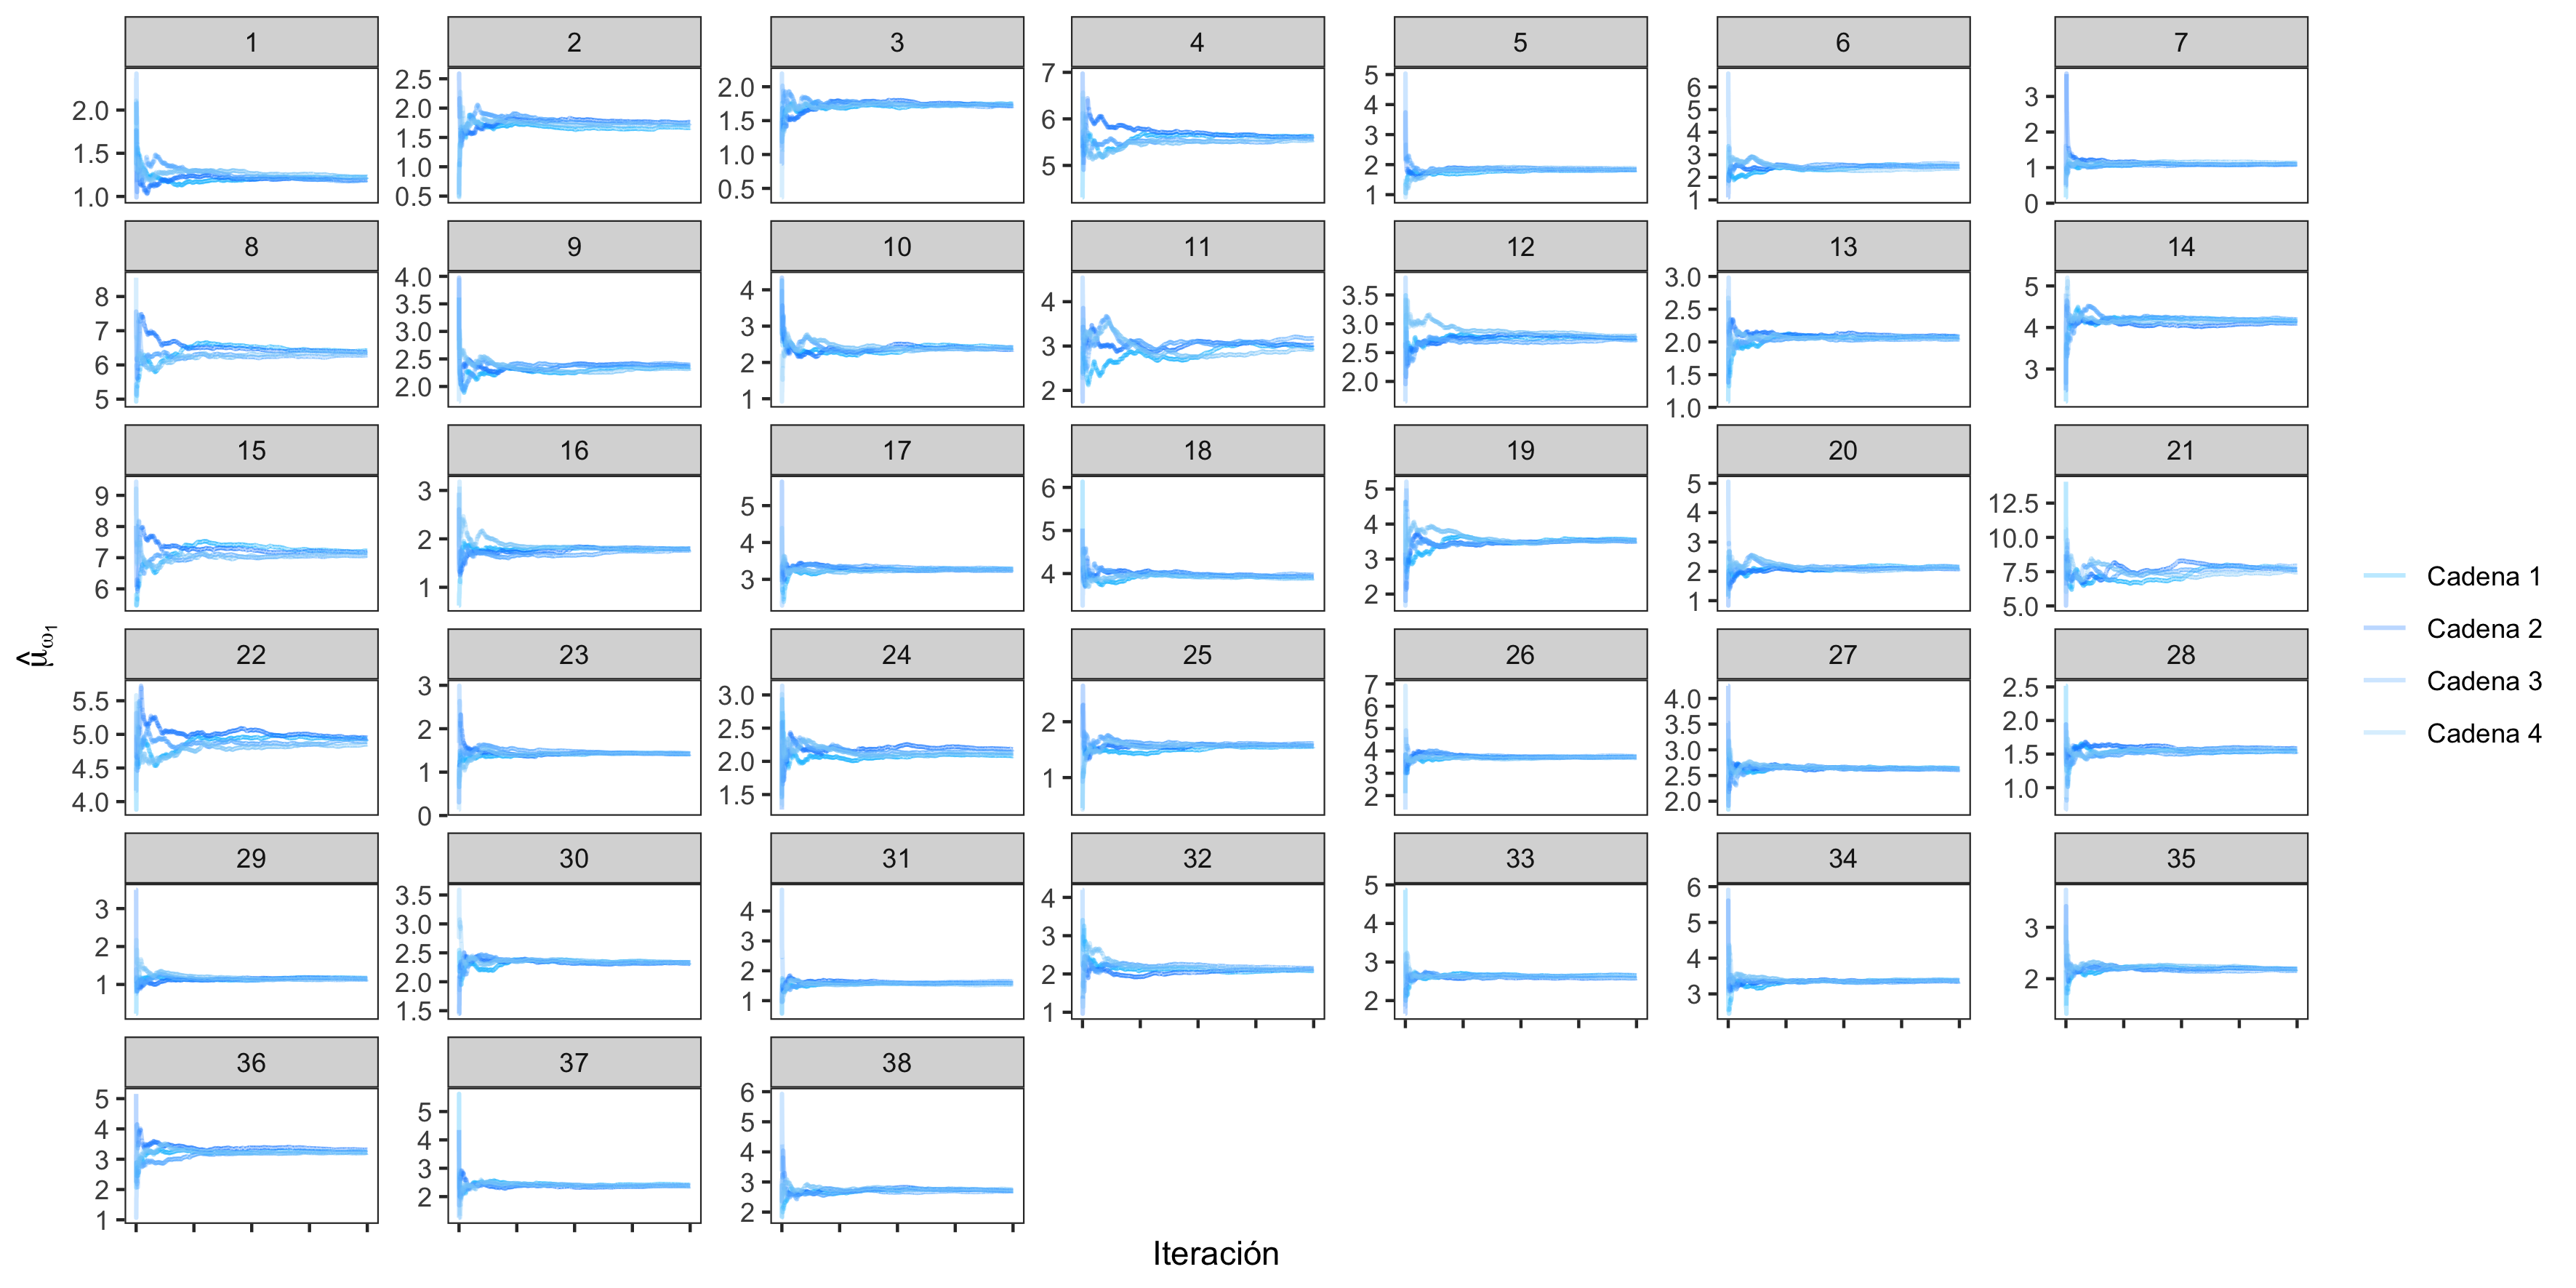
\includegraphics[width=10cm]{ergodic_means_omega1.png}
\caption{Gráfica de $\hat{\mu}_{\omega_1}$ a través de las iteraciones.}
\label{fig:ergodic_means_omega1}
\end{figure}

\begin{figure}
\centering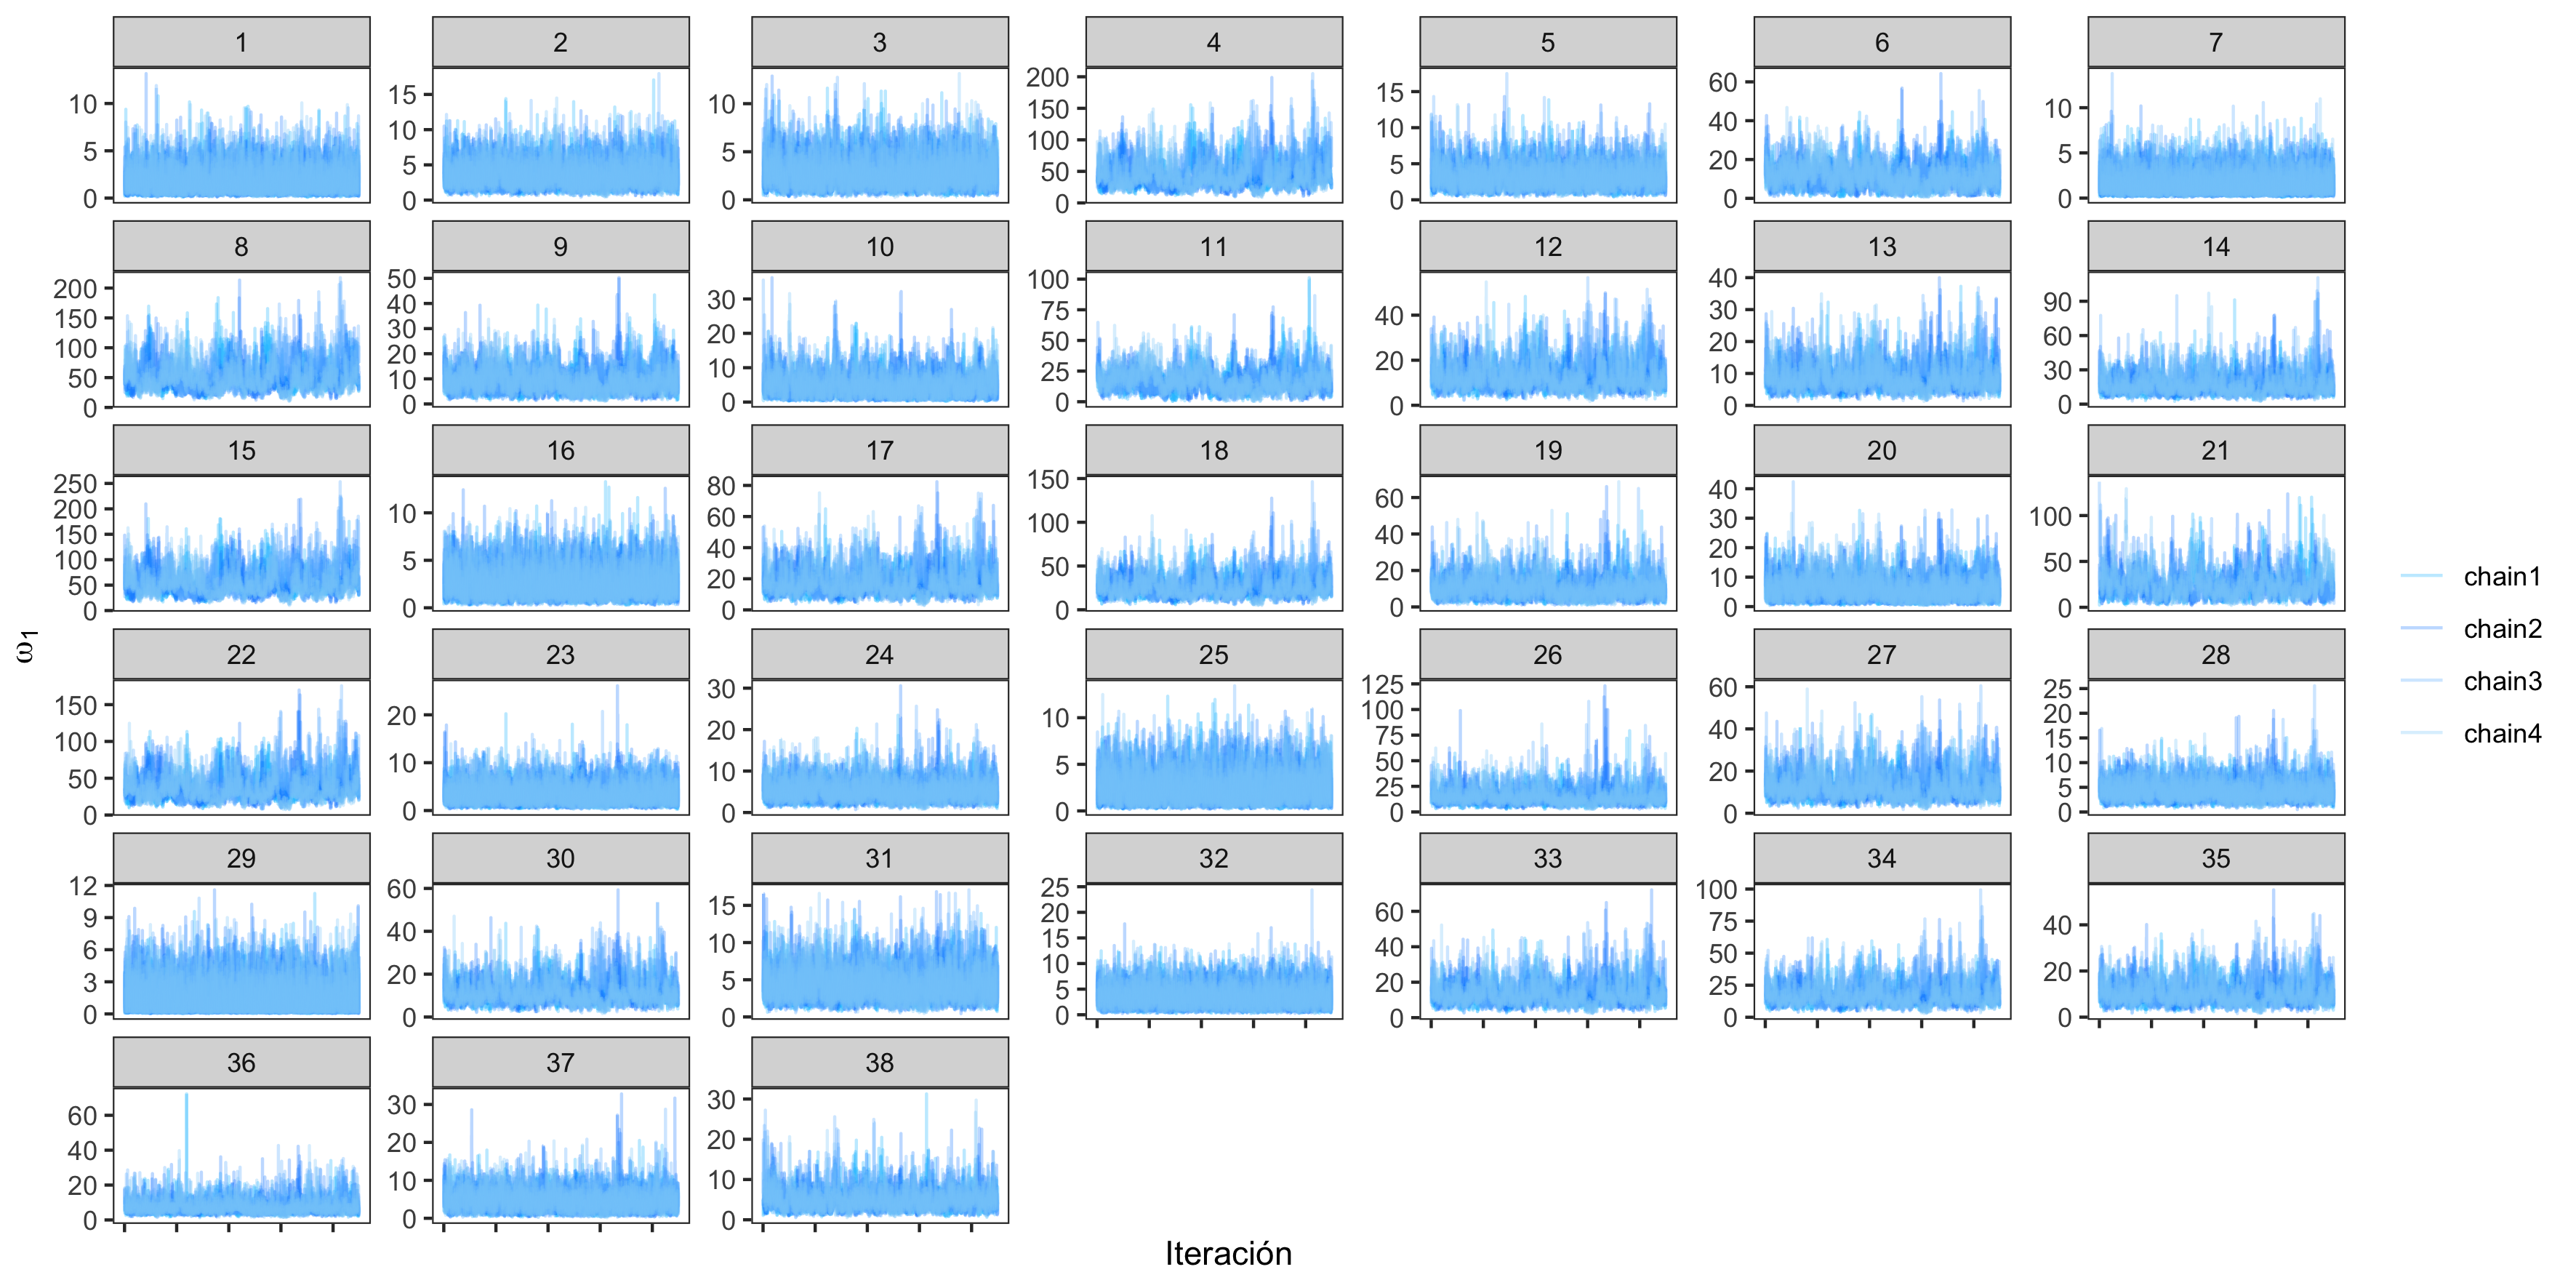
\includegraphics[width=10cm]{traceplots_omega1.png}
\caption{Valores simulados de $\omega_1$.}
\label{fig:traceplot_omega1}
\end{figure}

\begin{figure}
\centering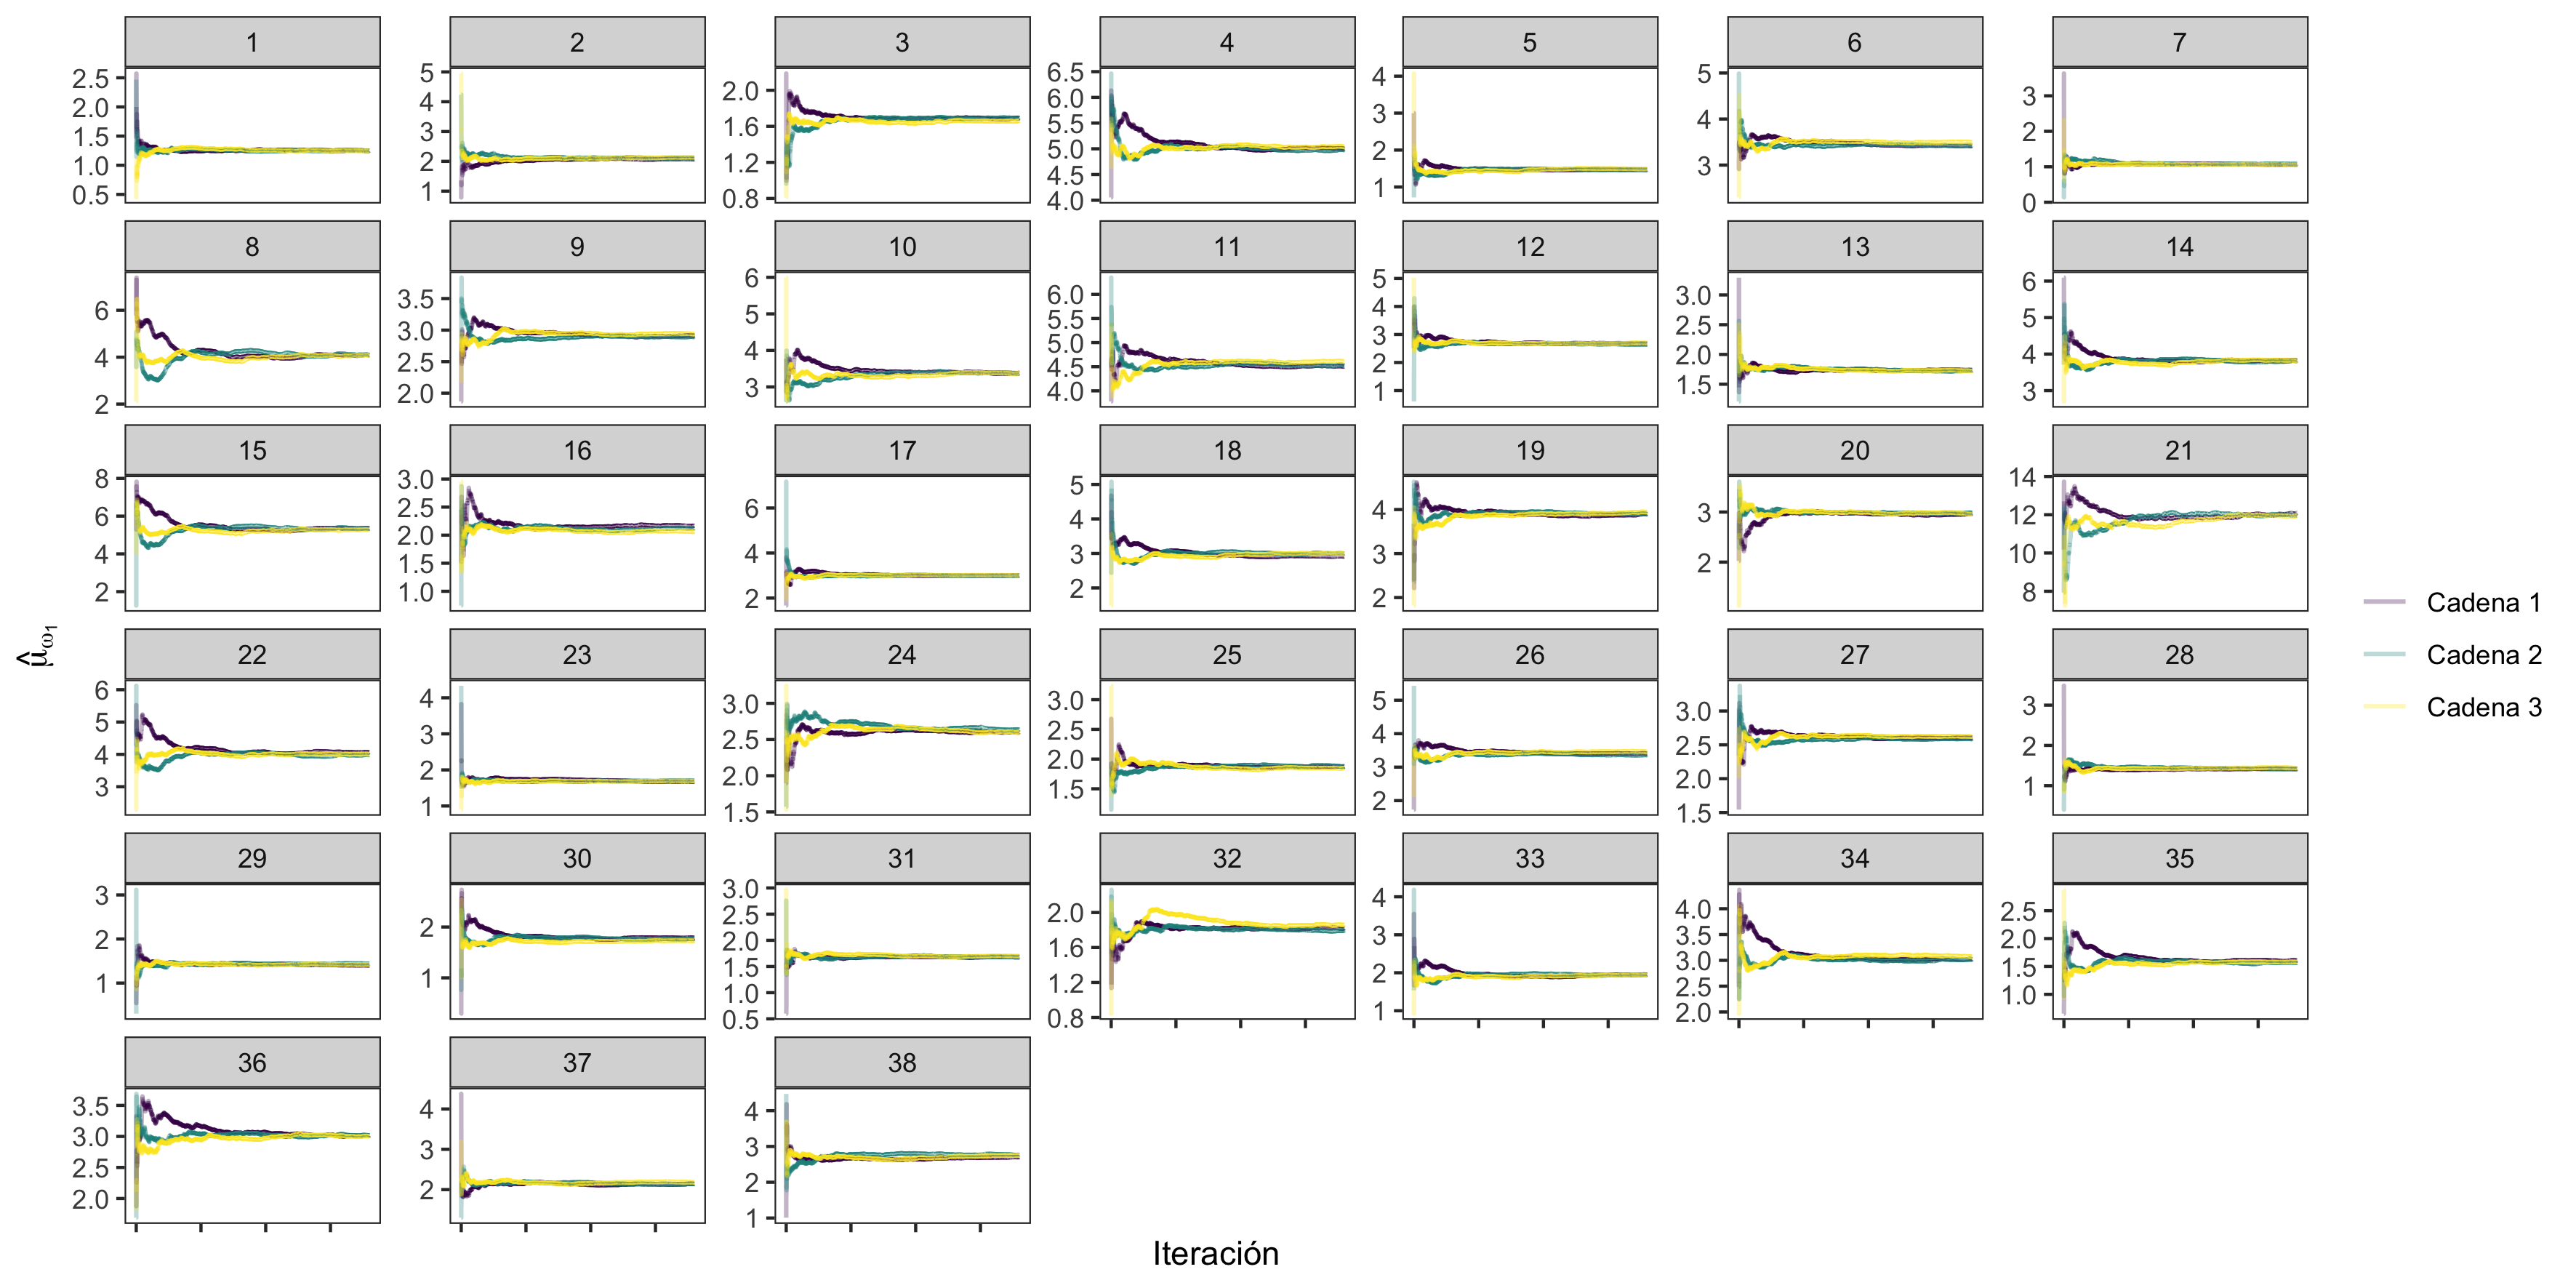
\includegraphics[width=10cm]{ergodic_means_omega2.png}
\caption{Gráfica de $\hat{\mu}_{\omega_2}$ a través de las iteraciones.}
\label{fig:ergodic_means_omega2}
\end{figure}

\begin{figure}
\centering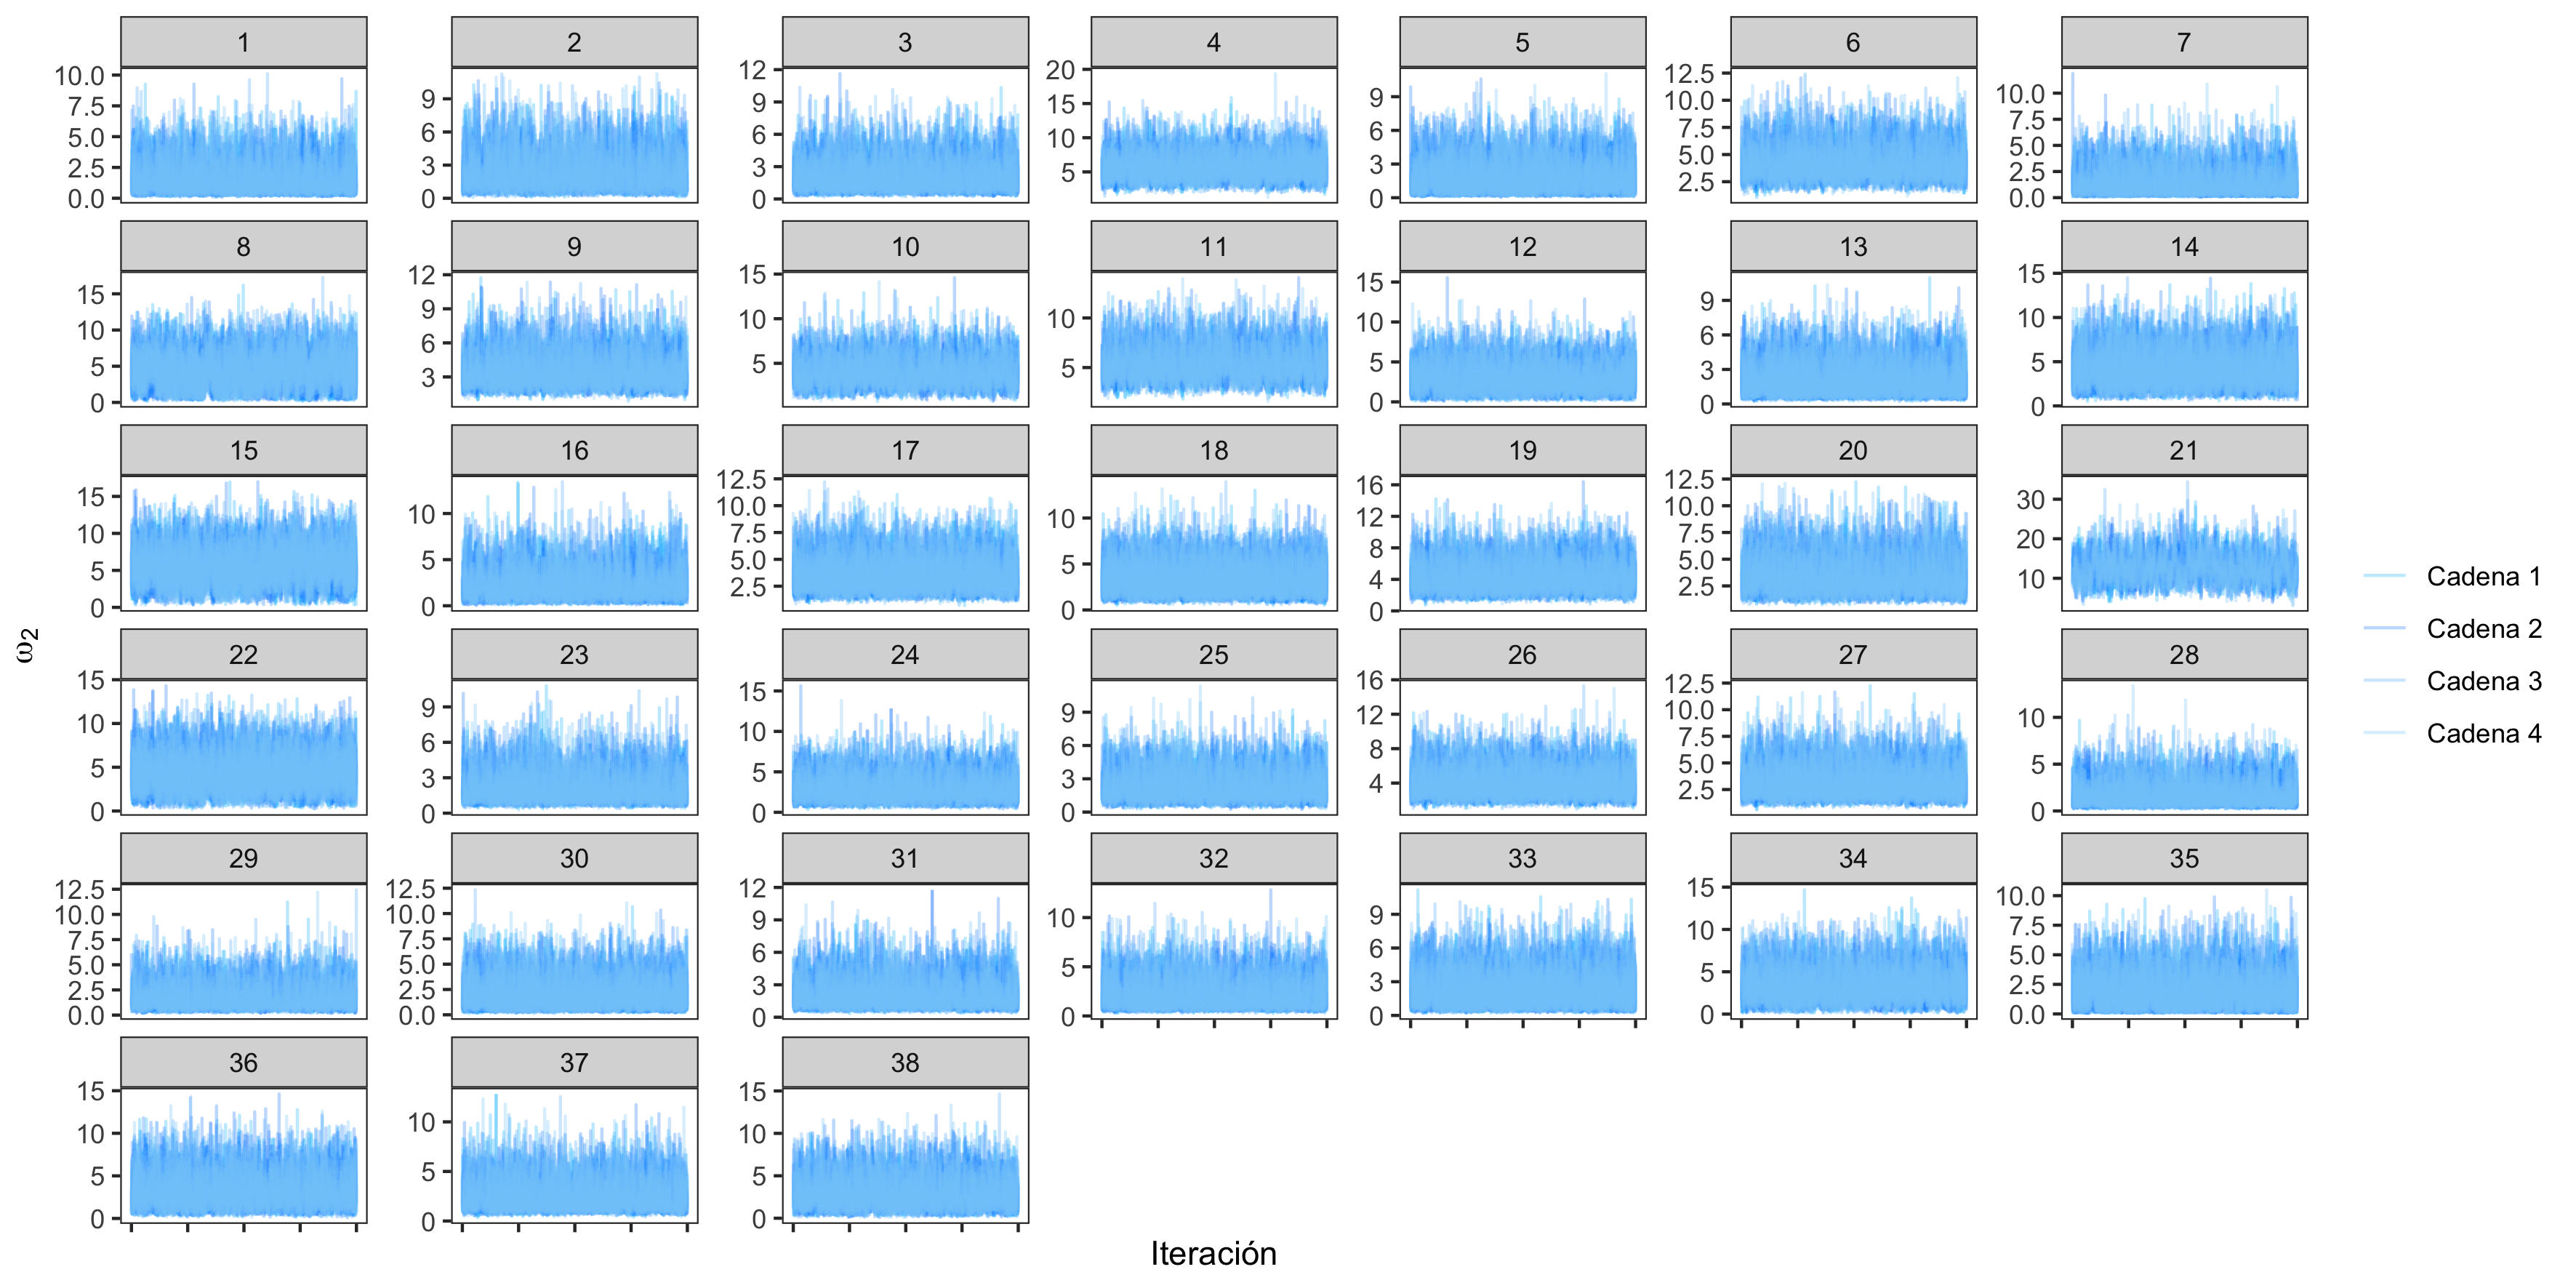
\includegraphics[width=10cm]{traceplots_omega2.png}
\caption{Valores simulados de $\omega_2$.}
\label{fig:traceplot_omega2}
\end{figure}

En las figuras \ref{fig:traceplot_omega1} y \ref{fig:traceplot_omega2} se encuentran los \textit{trace plots} de cada componentes de los vectores $\omega_1$ y $\omega_2$. Como se mencionó en la sección \ref{sec:mh}, el hecho de que las cadenas se encimen sugiere que se alcanzó la convergencia a la distribución estacionaria y se pierde la dependencia de los valores iniciales.\\

Por otro lado, en las figuras \ref{fig:ergodic_means_omega1} y \ref{fig:ergodic_means_omega2} vemos que la estimación del valor esperado converge para las distintas cadenas, indicando un comportamiento deseable de nuestras simulaciones.\\

Veamos una gráfica con las estimaciones de la media de $\omega_1$ y $\omega_2$ para cada uno de los individuos en cada cadena. Un mayor valor de $\omega_i$ está relacionado con una mayor supervivencia, sin contar el efecto de las variables explicativas. Resalta el individuo número 21, el cual tiene un valor de $\omega_2$ mucho mayor a los demás pacientes. Esto se debe a que el individuo 21 presentó el mayor registro en $t_2$ por un amplio margen.\\

\begin{figure}
\centering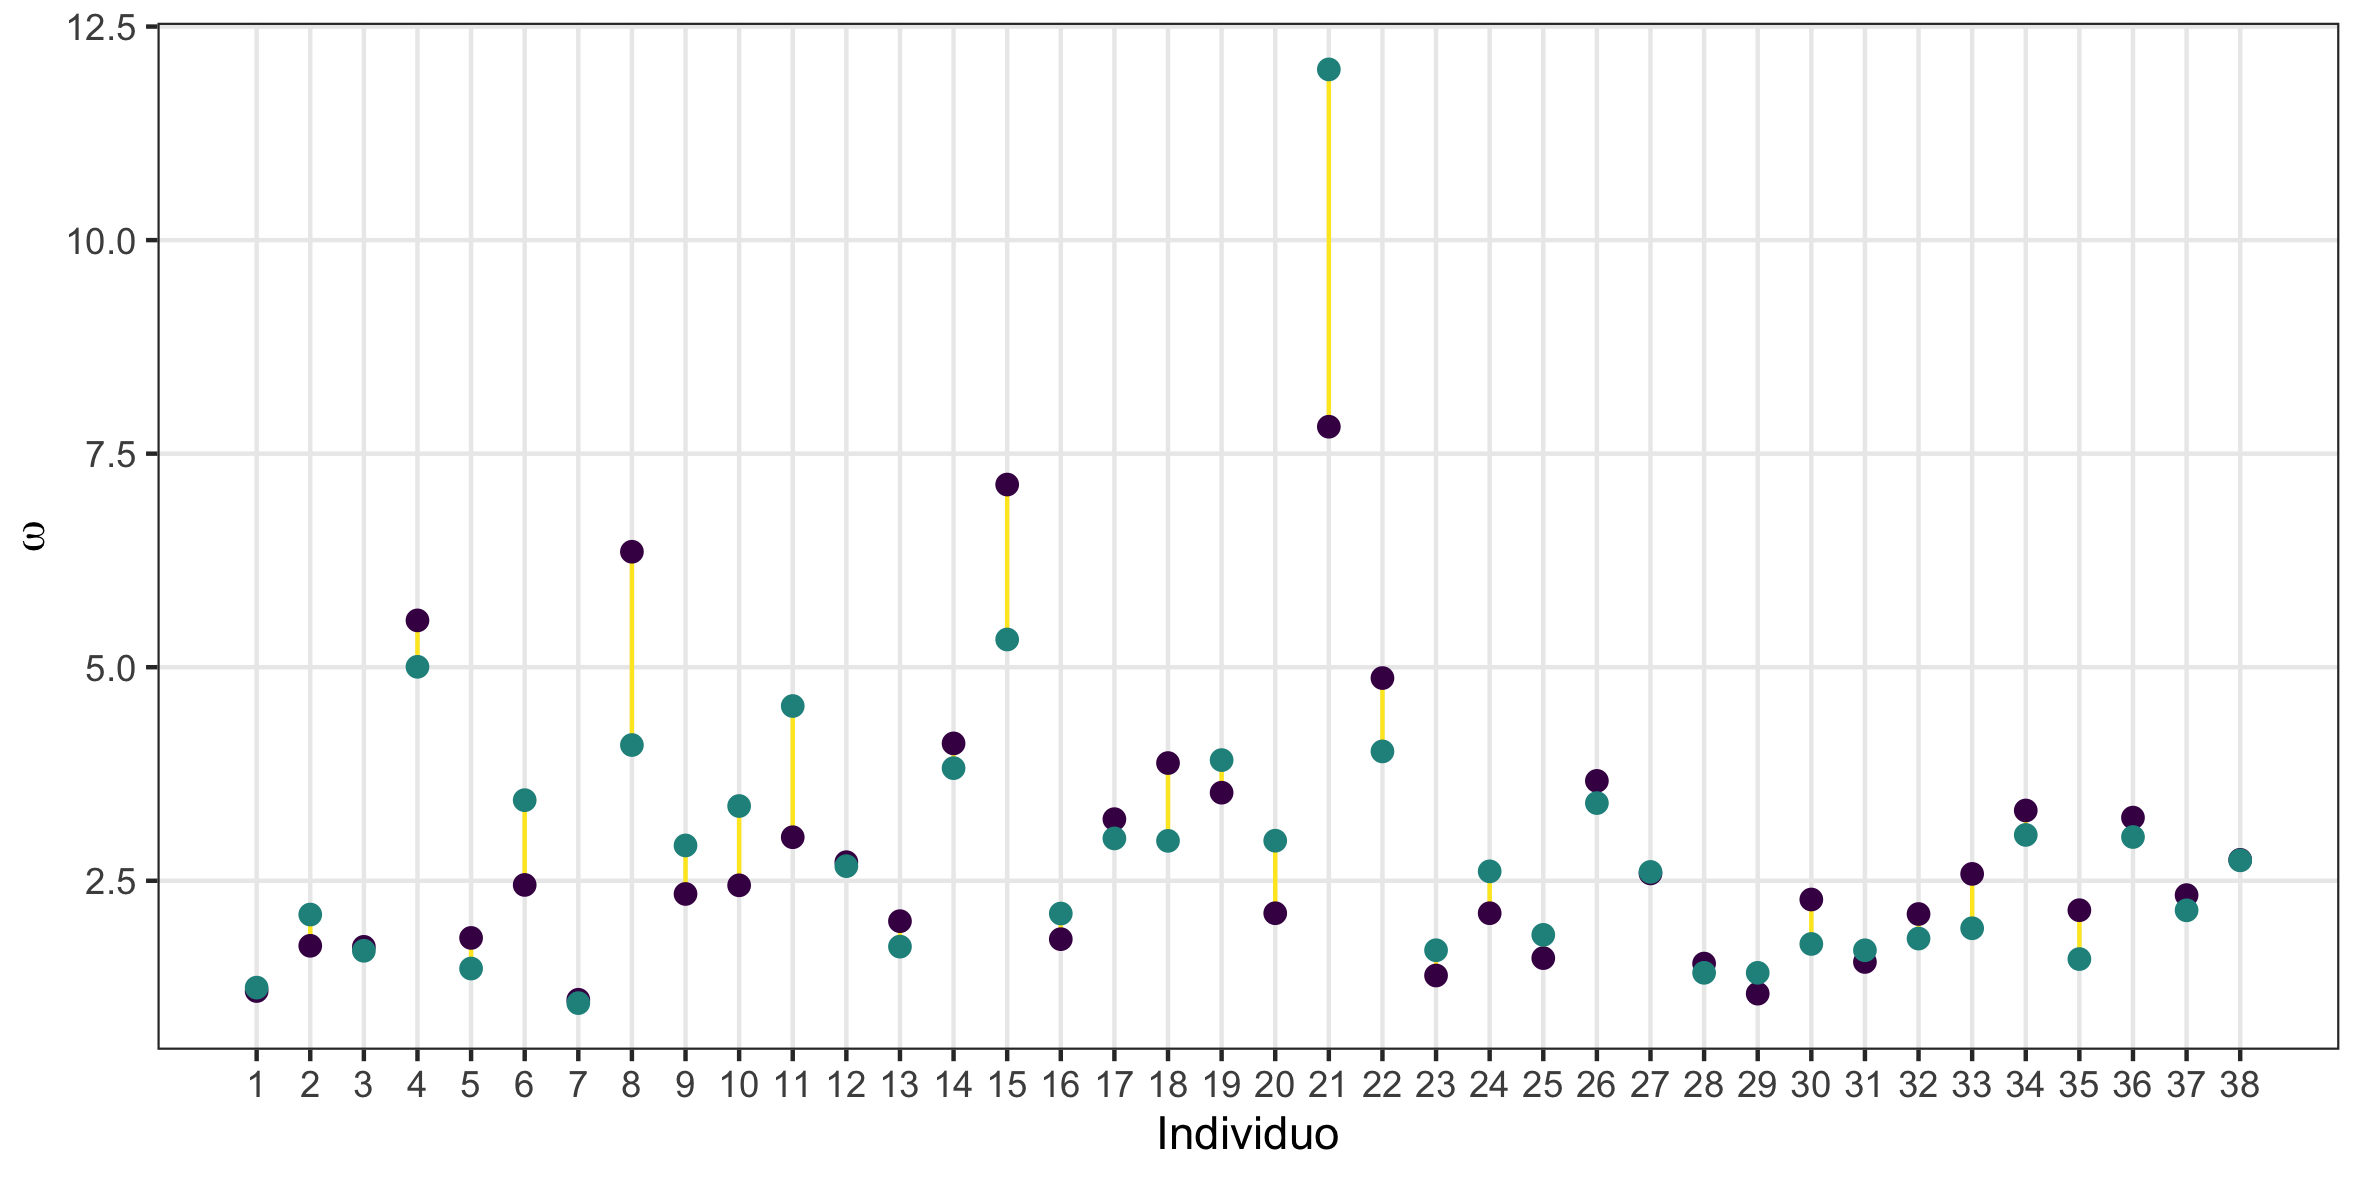
\includegraphics[width=10cm]{frailties.png}
\caption{Valores esperados de $\omega$ por individuo.}
\label{fig:frailties}
\end{figure}

Ahora examinemos las estimaciones de las tasas de riesgo base (correspondientes a los pacientes de sexo femenino) para cada una de las variables $T_1$ y $T_2$. En la gráfica se incluyen también bandas de confianza de 95 \%. Se puede apreciar el suavizamiento de las estimaciones que se obtiene por utilizar la distribución inicial no paramétrica. Mientras más chicos se hacen los intervalos de la partición del tiempo, más suaves se verán estas funciones. Es interesante notar que, al introducir correlación entre las tasas $\lambda_j$, tenemos estimaciones de la tasa de riesgo distintas de cero aún en los intervalos de tiempo en donde no se presentan eventos de fallo \citep{nieto}.\\

\begin{figure}
\centering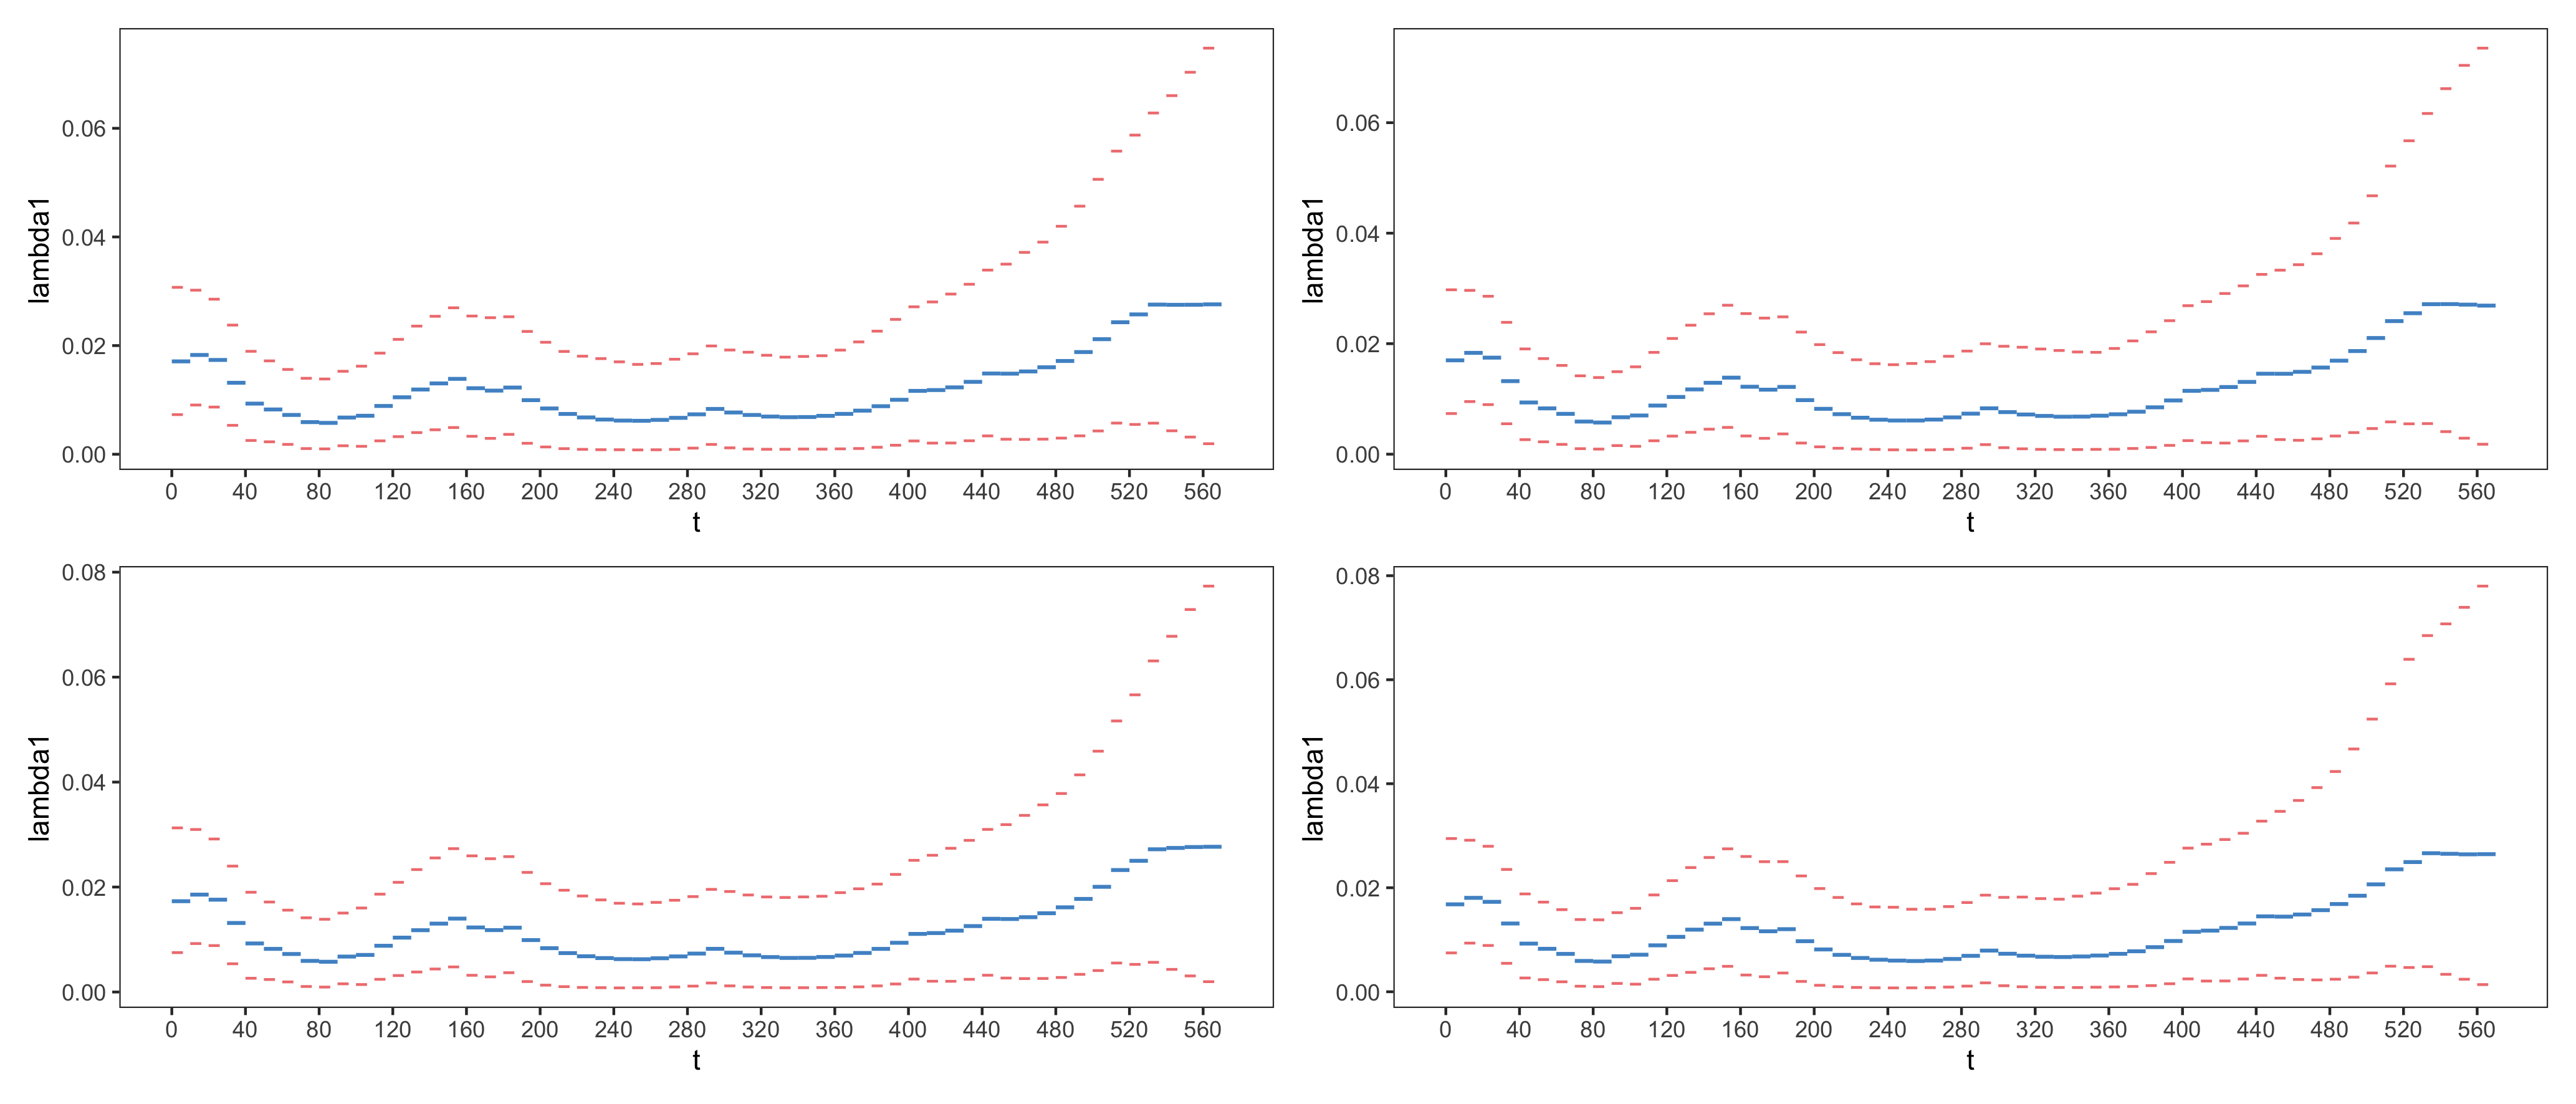
\includegraphics[width=10cm]{hazard1.png}
\caption{Valores esperados de la tasa de riesgo $\lambda_1$.}
\label{fig:haz_lambda1}
\end{figure}

\begin{figure}
\centering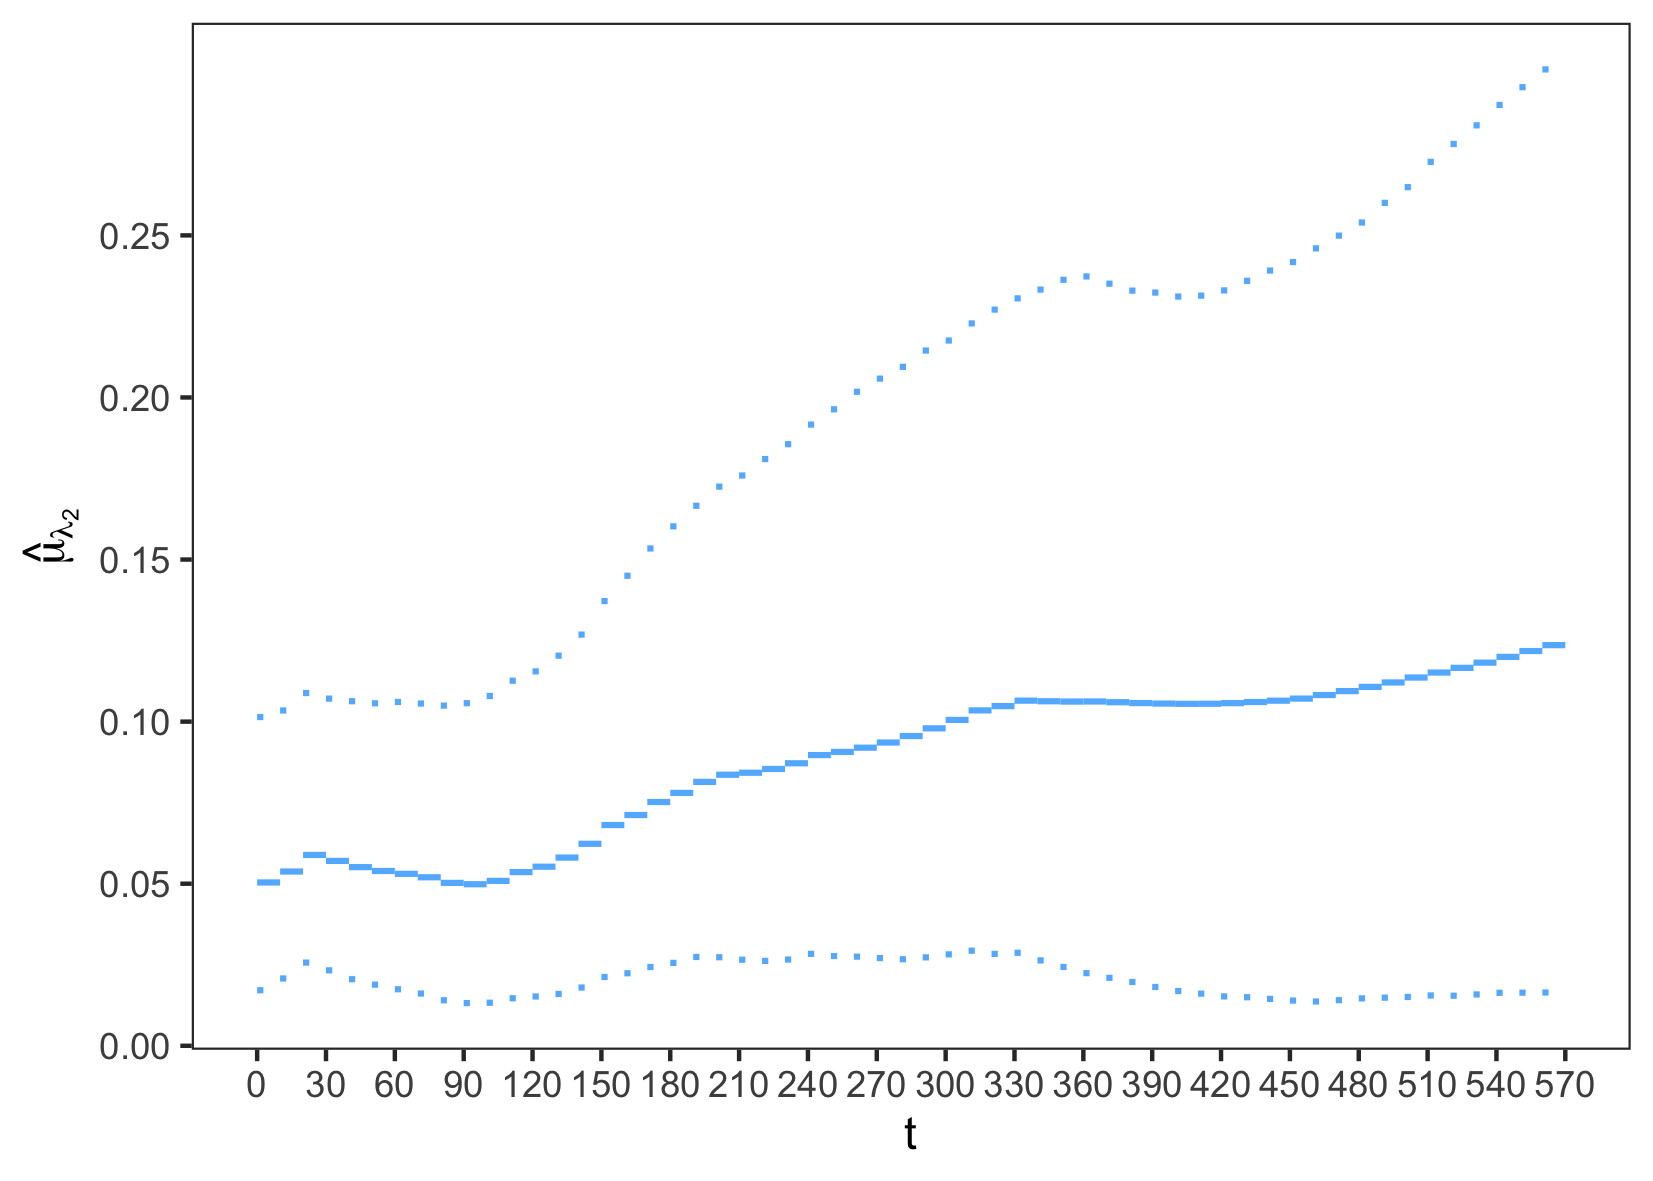
\includegraphics[width=10cm]{hazard2.png}
\caption{Valores esperados de la tasa de riesgo $\lambda_2$.}
\label{fig:haz_lambda2}
\end{figure}

Se incluyen también los diagnósticos para el parámetro $\gamma$ que modela la correlación entre los tiempos de fallo. El \textit{trace plot} sugiere que la distribución posterior es explorada de manera satisfactoria y la convergencia de las estimaciones de la media no señala ningún comportamiento indeseable.\\

\begin{figure}
\centering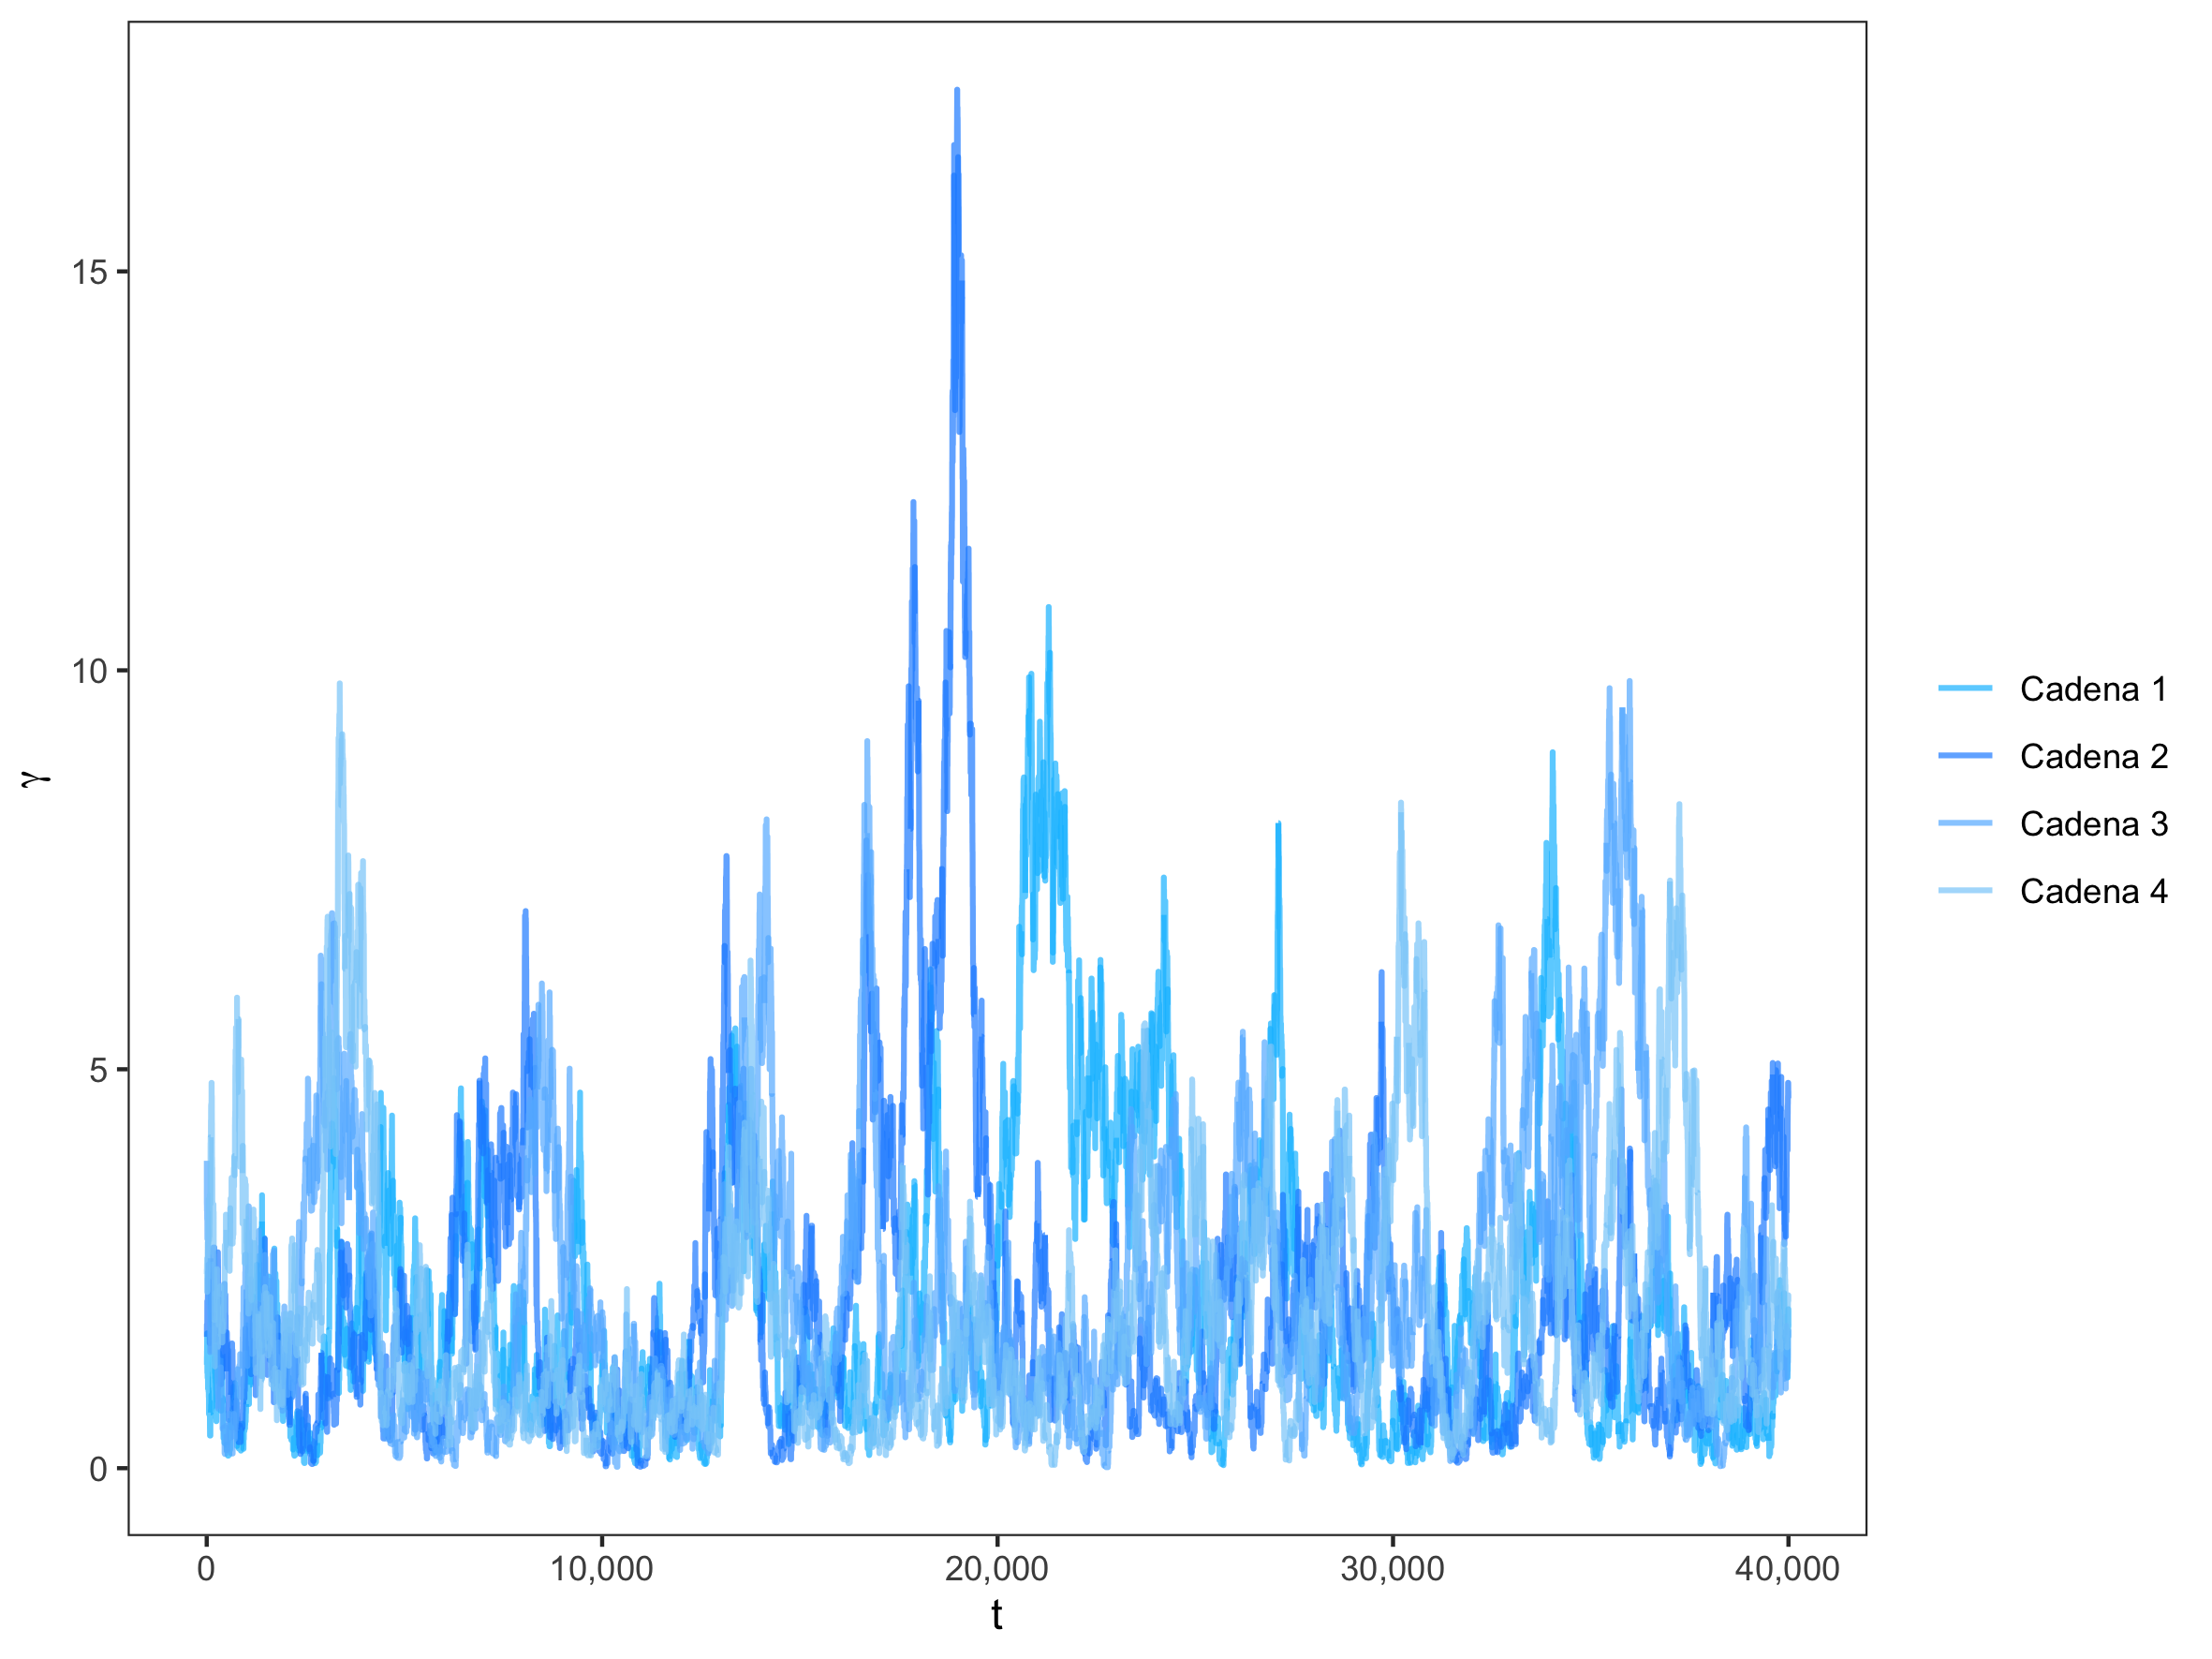
\includegraphics[width=10cm]{gamma_traceplot.png}
\caption{Valores simulados de $\gamma$.}
\label{fig:gamma_trace}
\end{figure}

\begin{figure}
\centering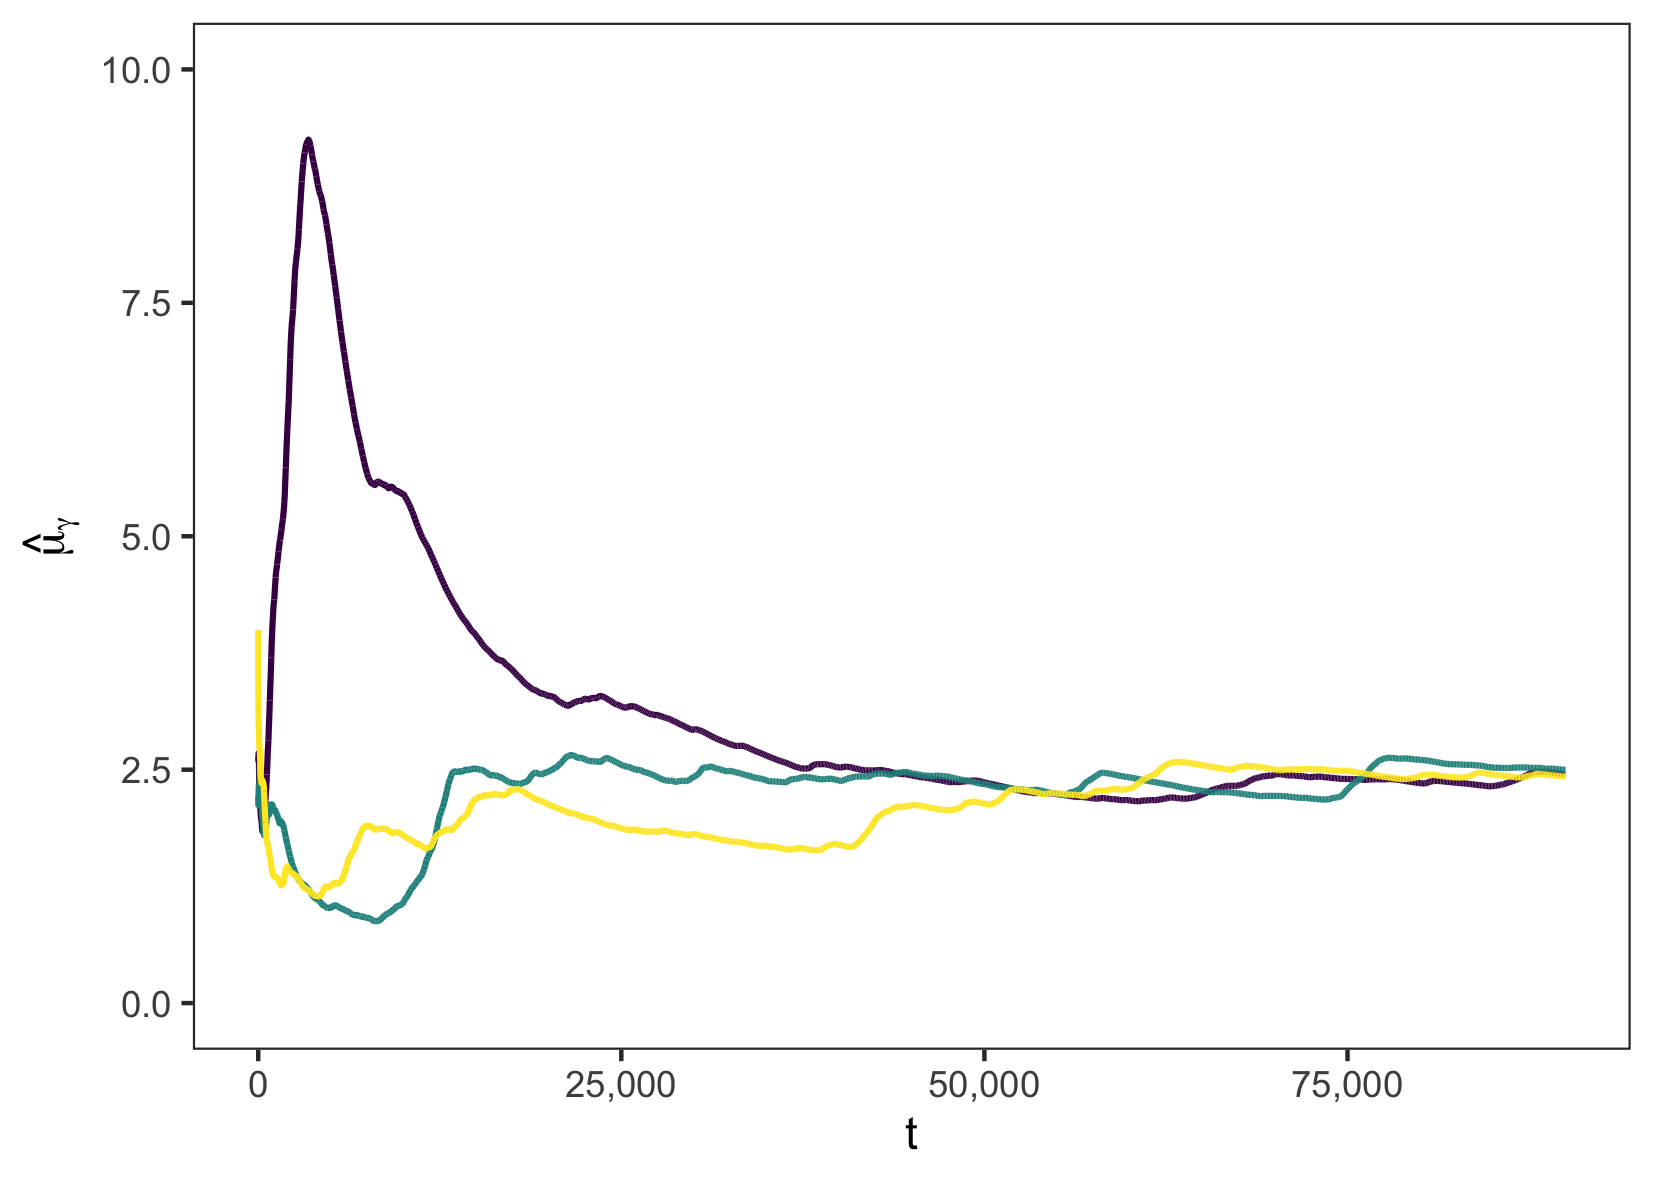
\includegraphics[width=10cm]{gamma_ergodic_means.png}
\caption{Evolución de $\hat{\mu}_{\gamma}$ en cada iteración.}
\label{fig:gamma_means}
\end{figure}

También se presenta un suavizamiento de los histogramas utilizando la función \texttt{geom\_density} del paquete \texttt{ggplot2} \citep{ggplot}. Podemos ver que las densidades de las cuatro cadenas son bastante parecidas, lo que sugiere que las observaciones fueron simuladas de la misma distribución.\\

\begin{figure}
\centering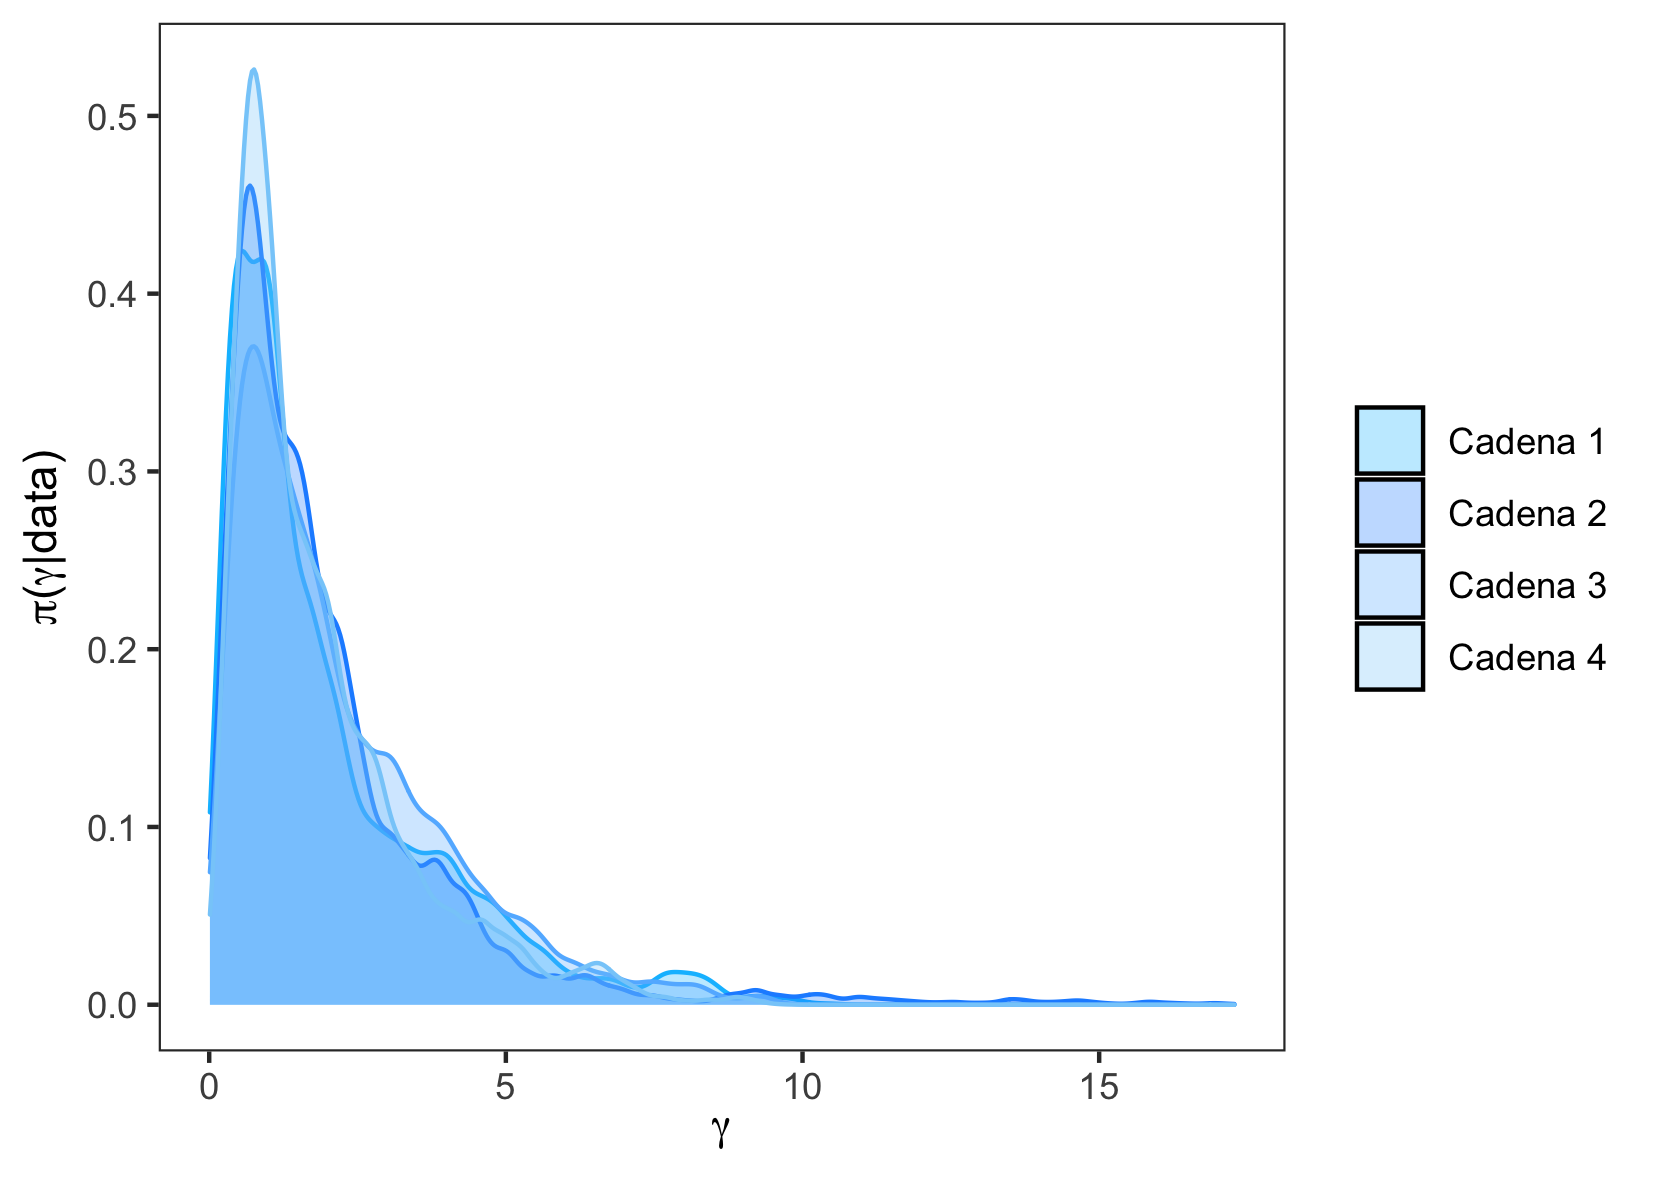
\includegraphics[width=10cm]{gamma_densities.png}
\caption{Suavizamiento con kernel gaussiano para $\pi (\gamma | data)$.}
\label{fig:gamma_densities}
\end{figure}

Para finalizar, veamos las simulaciones del parámetro $\theta$. Este parámetro está relacionado con la proporcionalidad de las tasas de riesgo entre pacientes de ambos sexos. Es decir, un coeficiente positivo indica que la tasa de riesgo es mayor para los hombres, mientras que un coeficiente negativo indica que esta tasa es mayor para las mujeres. Veamos primero el \textit{trace plot} de las cadenas en la figura \ref{fig:theta_trace}.\\

\begin{figure}
\centering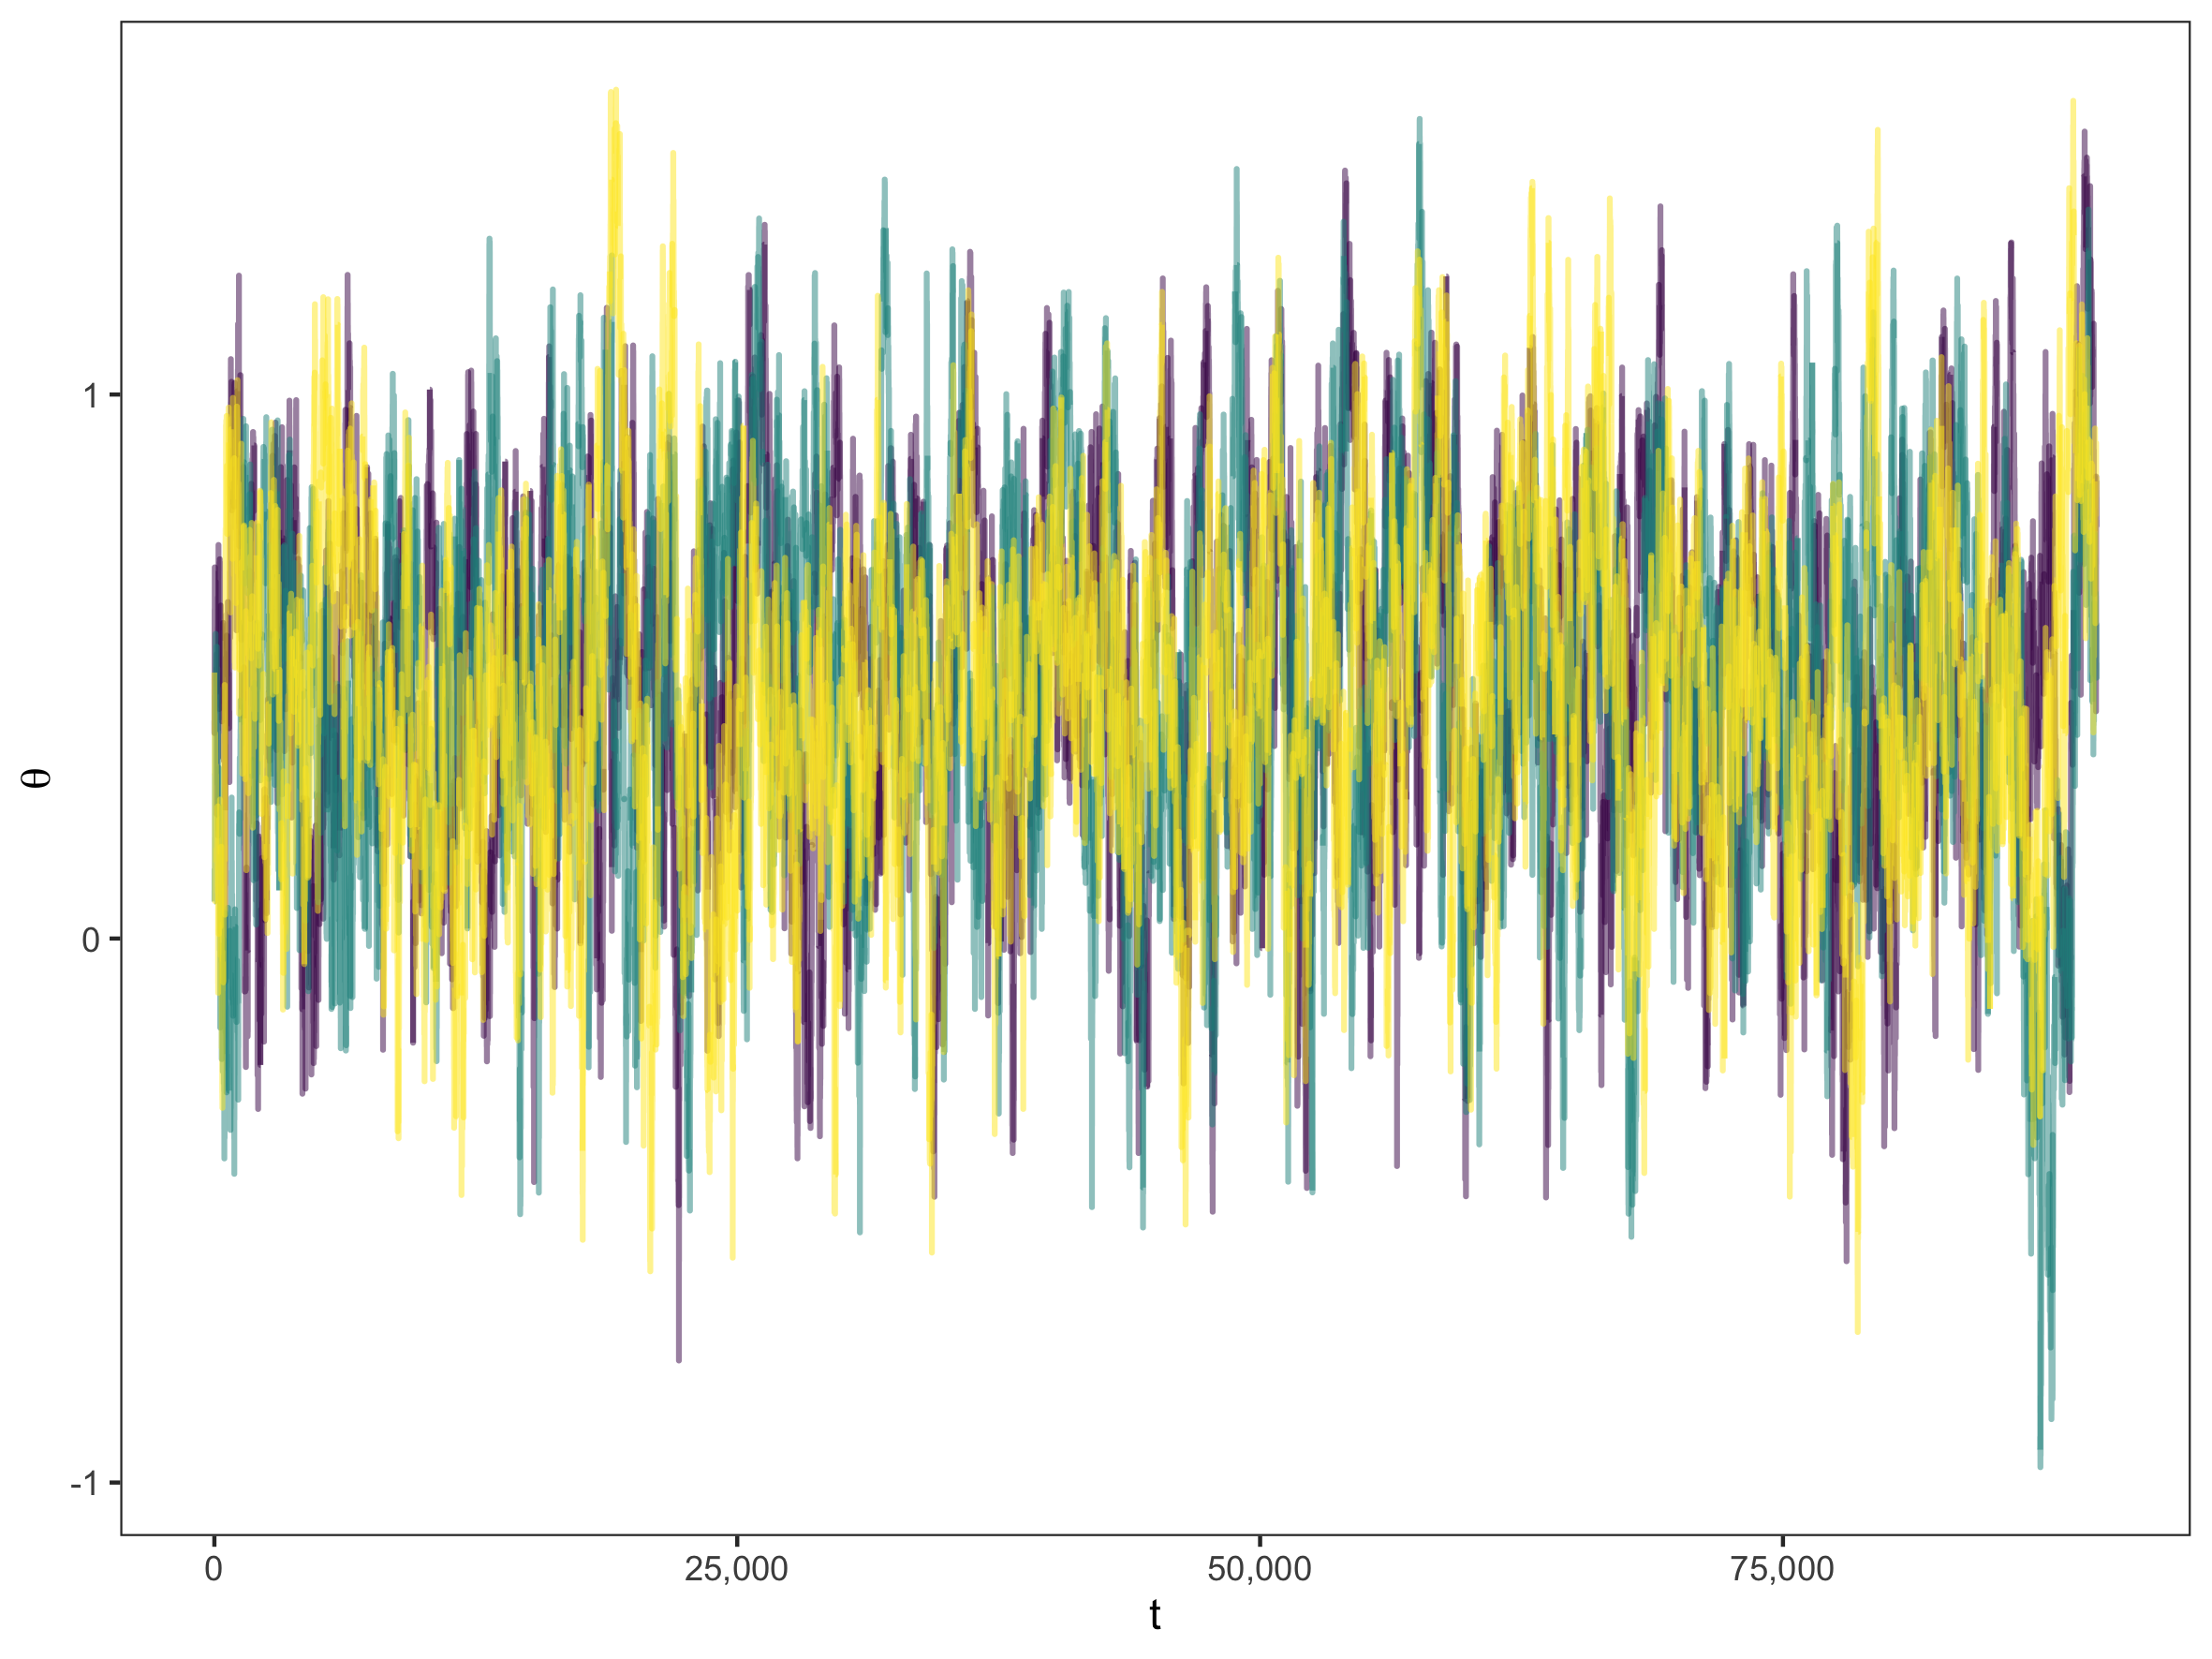
\includegraphics[width=10cm]{theta_traceplot.png}
\caption{Observaciones simuladas de $\theta$.}
\label{fig:theta_trace}
\end{figure}

Ahora veamos la estimación del valor esperado en cada iteración para cada cadena. Los valores esperados sugieren un efecto casi nulo del sexo del paciente sobre los tiempos de fallo (figura \ref{fig:theta_means}.\\

\begin{figure}
\centering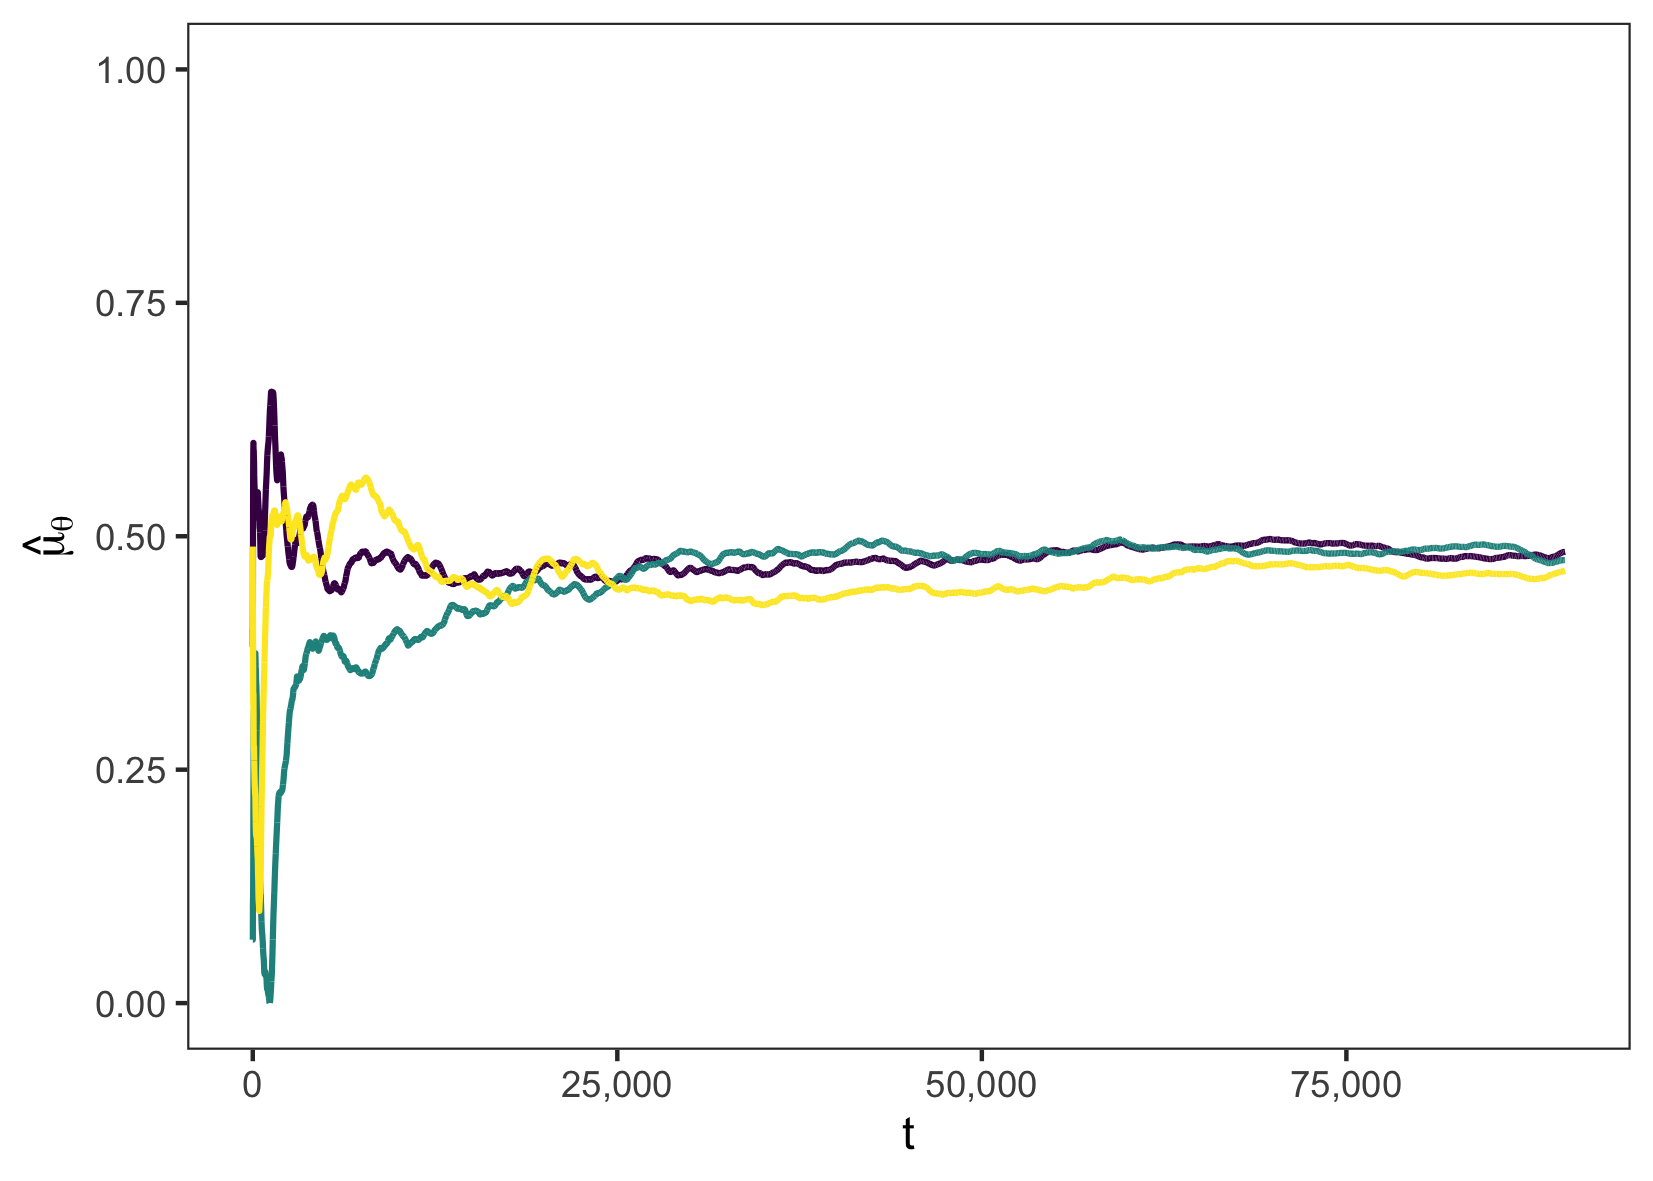
\includegraphics[width=10cm]{theta_ergodic_means.png}
\caption{Evolución de $\hat{\mu}_{\theta}$ en cada iteración.}
\label{fig:theta_means}
\end{figure}

La figura \ref{fig:theta_means} parece indicar que la convergencia de las estimaciones tarda más iteraciones que para los otros parámetros. Para confirmar esto, examinemos la gráfica de autocorrelación para las simulaciones de una de las cadenas.\\

\begin{figure}
\centering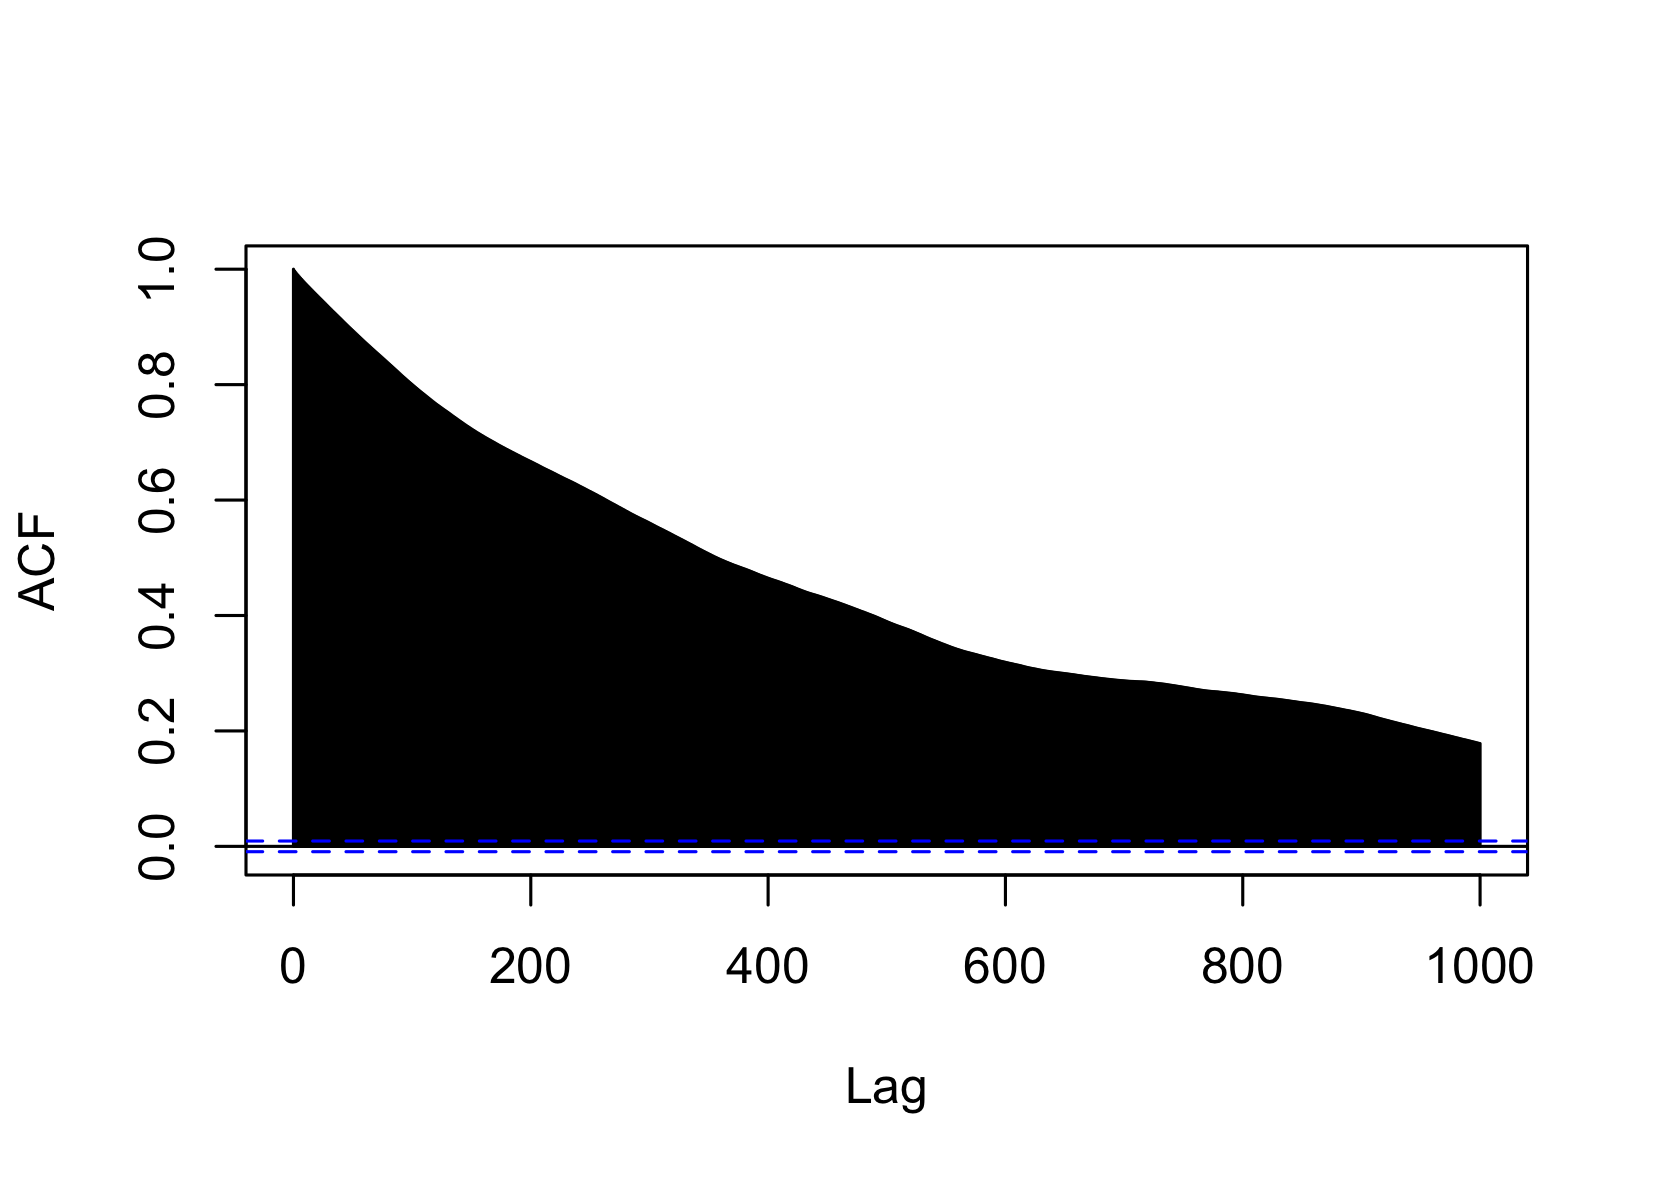
\includegraphics[width=10cm]{theta_acf.png}
\caption{Autocorrelación en las simulaciones de $\theta$.}
\label{fig:theta_acf}
\end{figure}

La figura \ref{fig:theta_acf} muestra que hay alta correlación entre las observaciones simuladas hasta un \textit{lag} de aproximadamente 400. Esto significa que la distribución posterior no es explorada de manera tan eficiente y las estimaciones tardan más tiempo en converger.\\

En la figura \ref{fig:theta_densities} se muestra el suavizamiento de los histogramas con la función \texttt{geom\_density}. Estos suavizamientos no muestran ningún comportamiento indeseable en las cadenas. Para disminuir la autocorrelación, se podrían modificar los parámetros de la función \texttt{bsbshaz\_sample} para cambiar las propuestas de algoritmo de Metropolis-Hastings. Para este trabajo se probó con varios valores distintos y se presentaron los que mostraron mejor comportamiento de las simulaciones.\\

\begin{figure}
\centering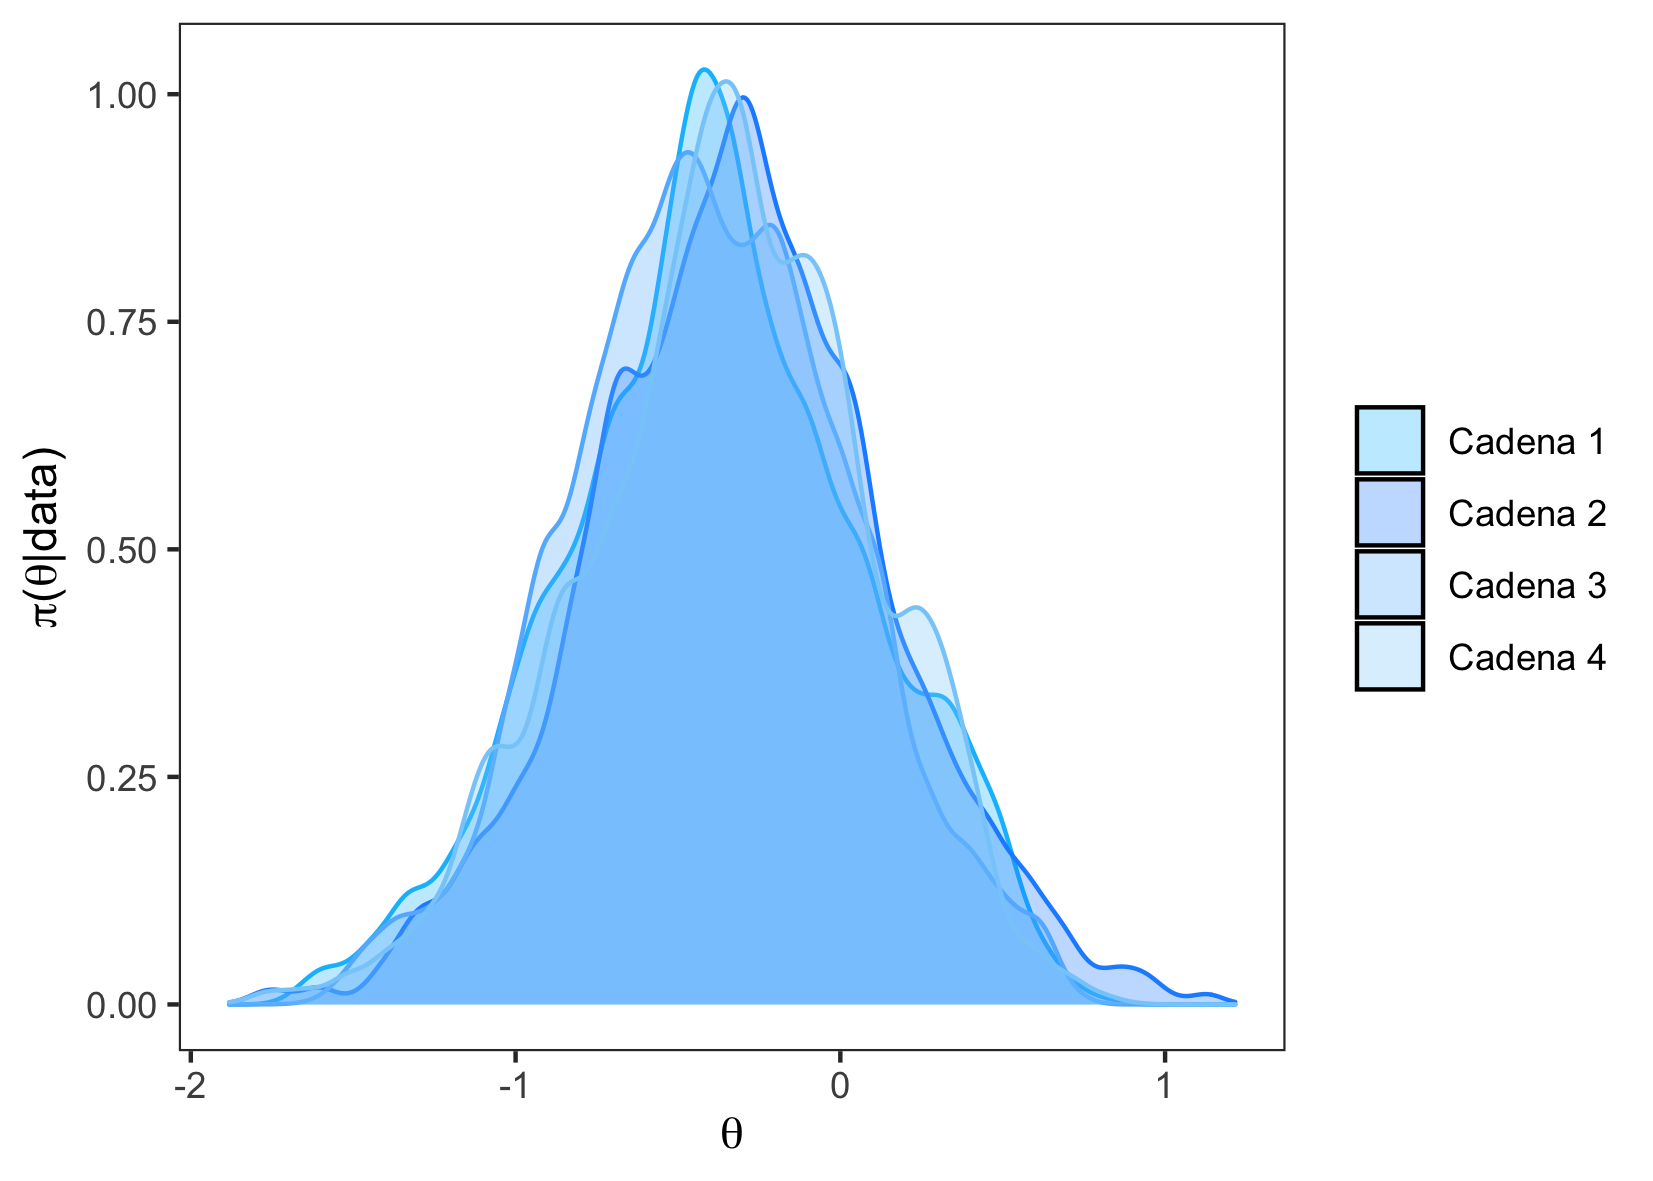
\includegraphics[width=10cm]{theta_densities.png}
\caption{Suavizamiento con kernel gaussiano para $\pi (\theta | data)$.}
\label{fig:theta_densities}
\end{figure}


Se podrían realizar diagnósticos para todos los parámetros involucrados en el modelo. Sin embargo, es opinión de quien escribe que lo aquí presentado ejemplifica bien el alcance del modelo y su implementación a través del paquete \texttt{BSBHaz}. Se invita al lector a utilizar el paquete, sugerir modificaciones y mejoras y señalar cualquier problema a través del sistema de \textit{pull requests} de Github \footnote{\url{https://docs.github.com/en/github/collaborating-with-issues-and-pull-requests}}.\\

\newpage

\section{Conclusión}

Repasemos los objetivos establecidos al principio de este trabajo. Estos fueron:
\begin{enumerate}
\item Introducir al lector a un modelo de datos de supervivencia bivariados titulado \textit{A Bayesian semi-parametric bivariate failure time model} por Luis E. Nieto-Barajas y Stephen G. Walker.\\
\item Presentar la elaboración de una herramienta para facilitar su uso y ampliar la disponibilidad.\\
\item Demostrar la variedad de cosas que se pueden hacer con R para que el lector se interese en utilizarlo.
\end{enumerate}

Para cumplir con estos objetivos se presentaron las bases teóricas necesarias en los capítulos \ref{analisis_sup} a \ref{sec_cadenas}, intercalando las explicaciones con ejemplos prácticos elaborados en R. En la sección \ref{elmodelo} se introdujo el modelo mencionado y se incluyó el código utilizado para obtener las simulaciones de cada una de las variables. Finalmente, en el apartado \ref{sec:ejemplo}, se introdujo el paquete \texttt{BSBHaz} creado específicamente para este trabajo y se presentó un ejemplo práctico con datos reales.\\

A pesar de que se cumplieron los objetivos, aún hay espacio para que el lector interesado aprenda más sobre estos temas e incluso pueda contribuir al desarrollo e implementación del paquete. A continuación se mencionan las principales áreas de oportunidad para lo aquí presentado.\\

Primero, sería interesante incorporar los algoritmos mencionados en la sección \ref{sec:mh} sobre Monte Carlo Hamiltoniano y el software Stan. Debido a la gran cantidad de parámetros que tiene el modelo, estos algoritmos podrían ayudar a explorar las distribuciones posteriores de una manera más efectiva y rápida.\\

Segundo, el paquete \texttt{BSBHaz} puede incluir nuevas funciones según los usuarios lo necesiten. Para esto, es necesario que se utilice el paquete, ya que de otra forma es imposible identificar áreas de oportunidad e incluso errores en los códigos. También se podrían modificar las funciones ya existentes para permitir mayor flexibilidad al usuario eligiendo colores y temas de las gráficas. También se podría incluir una función para obtener muestras de la distribución predictiva introducida en la sección \ref{elmodelo} y así obtener estimaciones muestrales para las medidas de concordancia del apartado \ref{sec_copulas}. Finalmente, este paquete se podría beneficiar mucho de computación paralela, lo cual permitiría distribuir las simulaciones en los distintos núcleos de una computadora y ahorrar tiempo en la ejecución.\\

Por último, quedan algunas deudas con aquel lector interesado en R. Primero, no se habló con mucho detalle de por qué las funciones se diseñaron en la manera en que se hizo. Un ejemplo es el uso de las funciones \texttt{map} del paquete \texttt{purrr} \citep{purrr} en vez de los iteradores usuales \texttt{for}. Para el lector que tenga algo de experiencia con R y le interese saber cómo funciona este lenguaje y por qué funciona como funciona, el libro \textit{Advanced R} de Hadley Wickham es un recurso esencial en opinión de quien escribe \citep{advanced_r}. Por el contrario, si el lector no tiene mucha experiencia con R y le gustaría poder utilizarlo para resolver problemas, el libro \textit{R for Data Science} de Hadley Wickham y Garrett Grolemund es su mejor acompañante \citep{rfordatascience}. Finalmente, no se habló en este trabajo del flujo de trabajo necesario para crear y publicar un paquete de R. Se recomienda a aquel lector interesado en este tema dirigirse al libro \textit{R Packages} de Hadley Wickham (¡qué sorpresa!) y Jennifer Bryan \citep{rpackages}.\\

Ojalá el lector haya quedado con ganas de utilizar el modelo y de programar más y mejor en R. El software libre como este lenguaje sobrevive y crece simplemente por el uso y la contribución de toda clase de personas, sin importar sus áreas de investigación, grados de estudio o intereses profiesionales. ¡UseR!

\newpage

\appendixtitleon
\appendixtitletocon
\begin{appendices}
\section{Densidad de una cópula} \label{densidad_copula}

Sean $X$ y $Y$ dos variables aleatorias continuas con función de distribución conjunta $F$ y marginales $F_X$ y $F_Y$. El teorema de Sklar \ref{sklar} nos dice que existe una única cópula $\C$ tal que $$F(x, y) = \C(F_X(x), F_Y(y)).$$\\

\begin{proposition}
Bajo las condiciones del Teorema de Sklar, la densidad conjunta de $X$ y $Y$, denotada $f$, está dada por $$\frac{\partial^2 F}{\partial y \partial x} = \partial c(F_X(x), F_Y(y))f_X(x)f_Y(y),$$ donde $\partial c$ es la densidad de la cópula $\C$, $f_X$ es la densidad marginal de $X$ y $f_Y$ la densidad marginal de $Y$.
\end{proposition} 

\begin{proof}
\begin{align*}
\frac{\partial F}{\partial x} &= \frac{\partial \C(F_X(x), F_Y(y))}{\partial x}\\\\
&= \frac{\partial \C}{\partial F_X} \frac{\partial F_X}{\partial x}\\\\
&= \frac{\partial \C}{\partial F_X}f_X(x)\\\\
\frac{\partial F}{\partial y \partial x} &= \frac{\partial}{\partial y} \left[\frac{\partial \C}{\partial F_X}f_X(x)\right]\\\\
&= \frac{\partial \C}{F_Y F_X}\frac{\partial F_Y}{\partial y}f_X(x)\\\\
&= \partial c (F_X(x), F_Y(y)) f_X(x) f_Y(y).\\
\end{align*}
\end{proof}

La notación $d\C(u, v)$ se refiere a la integral de Riemann-Stieltjes, una generalización de la integral de Riemann que se utiliza en la teoría de probabilidad para homologar notación entre distribuciones continuas y discretas. Si la función $F$ es una función de distribución continua con función de densidad $f(x) = \frac{d}{dx}F(x)$, $f(x) > 0 \ \forall x \in S_X$, se tiene que $$\int f(x) dx = \int dF(x)$$ (ver \citet{rudin}[p. 131]).\\

Si una cópula $\C$ tiene densidad dada por $\frac{\partial ^2}{\partial v \partial u} C(u, v)$, entonces $\C$ es absolutamente continua (ver \citet{nelsen}[p. 23]), por lo que $$\int\int \ d\C(u,v) = \int\int \partial c(u, v) \ dudv.$$\\

Para mayor información sobre integrales de Riemann-Stieltjes ver \citet{rudin} y \citet{bartle}.

\newpage

\section{Construcción de la cópula} \label{construccion_copula}

En este apéndice nos referimos a la ecuación \eqref{copula_modelo} de la sección \ref{elmodelo}. Del caso univariado \eqref{mezcla} se obtiene la expresión para las funciones de distribución marginales:

\begin{align*}
F(t) &= \int_0^t f(s) \ ds\\
&= \int_0^t\left(\int_0^\infty f(s|\omega)m(\omega) \ d\omega \right) \ ds\\
&= \int_0^t h(s)e^{-H(s)} \ ds\\
&= \int_0^{H(t)} e^{-u} \ du\\
&= 1-e^{-H(t)},
\end{align*}
por lo que, en el caso bivariado,
\begin{equation}\label{dist_marginal}
F_j(t) = 1-e^{-H_j(t)}.\\
\end{equation}

De las ecuaciones \eqref{mezcla_conjunta} y \eqref{indcon} se obtiene $$f(t_1, t_2) = \int_{H_1(t_1)}^\infty \int_{H_2(t_2)}^\infty \frac{h_1(t_1)}{\omega_1}\frac{h_2(t_2)}{\omega_2}m(\omega_1, \omega_2) \ d\omega_2 d\omega_1,$$ de donde podemos calcular la función de distribución conjunta $F(t_1, t_2)$.

\begin{align*}
F(t_1, t_2) &= \int_0^{t_1} \int_0^{t_2} f(s_1, s_2) \ ds_1 ds_2\\
&= \int_0^{t_1} \int_0^{t_2}\int_{H_1(s_1)}^\infty \int_{H_2(s_2)}^\infty \frac{h_1(s_1)}{\omega_1}\frac{h_2(s_2)}{\omega_2}m(\omega_1, \omega_2) \ d\omega_2 d\omega_1\\
&= \int_0^{t_1}\int_{H_1(s_1)}^\infty \frac{h_1(s_1)}{\omega_1}\left(\int_0^{t_2} \int_{H_2(s_2)}^\infty \frac{h_2(s_2)}{\omega_2} m(\omega_1, \omega_2) \ d\omega_2 ds_2 \right) d\omega_1 ds_1.
\end{align*}

Para desarrollar $$I_1 = \int_0^{t_2} \int_{H_2(s_2)}^\infty \frac{h_2(s_2)}{\omega_2} m(\omega_1, \omega_2) \ d\omega_2 ds_2$$ cambiamos el orden de integración y obtenemos

\begin{align*}
I_1 &= \int_0^{H_2(t_2)}\int_0^{H_2^{-1}(\omega_2)} \frac{h_2(s_2)}{\omega_2}m(\omega_1, \omega_2) \ ds_2 d\omega_2 \ +\\
& \ \ \ \int_{H_2(t_2)}^\infty \int_0^{t_2} \frac{h_2(s_2)}{\omega_2}m(\omega_1, \omega_2) \ ds_2 d\omega_2\\
&= \int_0^{H_2(t_2)} m(\omega_1, \omega_2) \ d\omega_2 \ + \ \int_{H_2(t_2)}^\infty \frac{H_2(t_2)}{\omega_2}m(\omega_1, \omega_2) \ d\omega_2.
\end{align*}

Ahora veamos que
\begin{align*}
&m(\omega_1) = \int_0^\infty m(\omega_1, \omega_2) \ d\omega_2 = \int_0^{H_2(t_2)} m(\omega_1, \omega_2) \ d\omega_2 \ + \ \int_{H_2(t_2)}^\infty m(\omega_1, \omega_2) \ d\omega_2\\
&\implies \int_0^{H_2(t_2)} m(\omega_1, \omega_2) \ d\omega_2 = m(\omega_1) - \int_{H_2(t_2)}^\infty m(\omega_1, \omega_2) \ d\omega_2\\
&\implies I_1 = m(\omega_1) + \int_{H_2(t_2)}^\infty m(\omega_1, \omega_2) \left( \frac{H_2(t_2)}{\omega_2}-1\right) \ d\omega_2,\\
\end{align*}

por lo que, regresando a $F(t_1, t_2)$ tenemos que

\begin{align*}
F(t_1, t_2) &= \int_0^{t_1} \int_{H_1(s_1)}^\infty \frac{h_1(s_1)}{\omega_1}\left( I_1 \right) \ d\omega_1 ds_1\\
&= \int_0^{t_1} \frac{h_1(s_1)}{\omega_1}m(\omega_1) \ d\omega_1 ds_1 \ +\\ & \ \ \ \int_{H_2(t_2)}^\infty \left(\frac{H_2(t_2)}{\omega_2}-1 \right) \left(\int_0^{t_1}\int_{H_1(s_1)}^\infty \frac{h_1(s_1)}{\omega_1}m(\omega_1, \omega_2) \ d\omega_1 ds_1 \right) d\omega_2\\
&= F_1(t_1) \ + \\
& \ \ \ \int_{H_2(t_2)}^\infty \left(\frac{H_2(t_2)}{\omega_2}-1 \right)\left(m(\omega_2) + \int_{H_1(t_1)}^\infty m(\omega_1, \omega_2) \left(\frac{H_1(t_1)}{\omega_1}-1 \right) \ d\omega_1 \right) d\omega_2\\
&= F_1(t_1) \ + \ \int_{H_2(t_2)}^\infty m(\omega_2) \left( \frac{H_2(t_2)}{\omega_2}-1 \right) \ d\omega_2 \ +\\
& \ \ \ \int_{H_2(t_2)}^\infty\int_{H_1(t_1)}^\infty \left(\frac{H_2(t_2)}{\omega_2}-1\right)\left(\frac{H_1(t_1)}{\omega_1}-1\right) m(\omega_1, \omega_2) \ d\omega_1 d\omega_2\\
&= F_1(t_1) + F_2(t_2) - 1 \ +\\
& \ \ \ \int_{H_2(t_2)}^\infty\int_{H_1(t_1)}^\infty \left(\frac{H_2(t_2)}{\omega_2}-1\right)\left(\frac{H_1(t_1)}{\omega_1}-1\right) m(\omega_1, \omega_2) \ d\omega_1 d\omega_2.\\
\end{align*}

Como $H_j(t_j) = -\log (1-F_j(t_j))$, entonces se tiene que la función de distribución conjunta cumple $F(t_1, t_2) = C(F_1(t_1), F_2(t_2))$, donde $C$ es la función dada por
\begin{align} \label{eq:copula:original}
C(u, v) &= u \ + \ v \ - \ 1 \ + \nonumber \\
& \ \ \ \int_{-\log (1-u)}^\infty \int_{-\log (1-v)}^\infty \left( \frac{\log (1-u)}{\omega_1}+1 \right) \left( \frac{\log (1-v)}{\omega_2}+1\right) m(\omega_1, \omega_2) \ d\omega_2 d\omega_1.
\end{align}

Para obtener la cópula de supervivencia \eqref{copula_modelo}, aplicamos el resultado \ref{def_cop_surv} y conluimos que $$S(t_1, t_2) = C(S_1(t_1), S_2(t_2)),$$ donde $C$ es la función dada por $$C(u, v) = \int_{-\log (u)}^\infty \int_{-\log (v)}^\infty \left( \frac{\log (u)}{\omega_1}+1 \right) \left( \frac{\log (v)}{\omega_2}+1\right) m(\omega_1, \omega_2) \ d\omega_2 d\omega_1.$$

\newpage

\section{Densidad de la cópula del modelo}
\label{sec_densidad_copula_modelo}

Buscamos obtener la densidad de la cópula \eqref{copula_distribucion}. Para esto utilizamos la regla de Leibniz para la derivada de una integral. Esta regla es:

\begin{align}\label{regla_leibniz}
\frac{d}{dx} \int_{a(x)}^{b(x)} f(x, t) \ dt &= f(x, b(x)) \frac{d}{dx}b(x) \ - \ f(x, a(x))\frac{d}{dx}a(x) \ + \nonumber\\
&\ \ \ \int_{a(x)}^{b(x)}\frac{\partial}{\partial x} f(x, t) \ dt
\end{align}

Los supuestos y la demostración se pueden encontrar en \citet{flanders}.\\

Recordemos la expresión para la cópula \eqref{copula_distribucion}
\begin{align*}
C(u, v) &= u \ + \ v \ - \ 1 \ +\\ 
& \ \ \ \int_{-\log (1-u)}^\infty \int_{-\log (1-v)}^\infty f(u, v, \omega_1, \omega_2) \ d\omega_2 d\omega_1,
\end{align*}
donde $f(u, v, \omega_1, \omega_2) = \left( \frac{\log (u)}{\omega_1}+1 \right) \left( \frac{\log (v)}{\omega_2}+1\right) m(\omega_1, \omega_2)$.\\

Aplicando \eqref{regla_leibniz} tenemos que
\begin{align*}
\frac{\partial C}{\partial u} &= 1 + \frac{\partial}{\partial u} \int_{-\log (1-u)}^\infty g_1(u, v, \omega_1, \omega_2) \ d\omega_1\\
&= 1 \ - \ g_1(u, v, -\log (1-u), \omega_2)\frac{\partial}{\partial u}\left[ -\log (1-u) \right] \ +\\
& \ \ \ \int_{-\log (1-u)}^{\infty} \frac{\partial}{\partial u}g_1(u, v, \omega_1, \omega_2) \ d\omega_1\\
&= \int_{-\log (1-u)}^\infty \int_{-\log (1-v)}^\infty \left(-\frac{1}{(1-u)\omega_1}\right)\left(1+\frac{\log (1-v)}{\omega_2}\right) m(\omega_1, \omega_2) \ d\omega_2 d\omega_1,
\end{align*}
donde $$g_1(u, v, \omega_1, \omega_2) = \int_{-\log (1-v)}^\infty \left(1+\frac{\log (1-u)}{\omega_1}\right)\left(1+\frac{\log (1-v)}{\omega_2}\right) m(\omega_1, \omega_2) \ d\omega_2$$ y $$g_1(u, v, -\log (1-u), \omega_2) = 0.$$\\

Así, aplicando otra vez \eqref{regla_leibniz} tenemos que
\begin{align*}
\frac{\partial C^2}{\partial v \partial u} &= \frac{\partial}{\partial v} \int_{-\log (1-v)}^\infty g_2(u, v, \omega_1, \omega_2) \ d\omega_2\\
&= -g_2(u, v, \omega_1, -\log (1-v))\frac{\partial}{\partial v}\left[ -\log (1-v)\right] \ +\\
&\ \ \ \int_{-\log (1-v)}^\infty \frac{\partial}{\partial v}g_2(u, v, \omega_1, \omega_2) \ d\omega_2\\
&= \int_{-\log (1-u)}^\infty \int_{- \log (1-v)}^\infty \left(\frac{1}{(1-u)\omega_1}\right)\left(\frac{1}{(1-v)\omega_2}\right) m(\omega_1, \omega_2) \ d\omega_2 d\omega_1.\\
\end{align*}

Por lo que $$\partial c(u, v) = \int_{-\log (1-u)}^\infty \int_{- \log (1-v)}^\infty \left(\frac{1}{(1-u)\omega_1}\right)\left(\frac{1}{(1-v)\omega_2}\right) m(\omega_1, \omega_2) \ d\omega_2 d\omega_1.$$

\newpage

\section{Códigos de R}
\subsection{Ejemplo de verosimilitud exponencial}
\label{ap:lik}

\begin{lstlisting}
nsim <- 10000
lambda <- 0.1

set.seed(42)

time.samples <- rexp(n = nsim, rate = lambda)

# Suponemos que el monitoreo termino en T = 15

time.censored <- ifelse(time.samples > 15, 15, time.samples)
delta <- ifelse(time.samples > 15, 0, 1)

log_lik <- function(lambda) {
  sum(delta) * log(lambda) - lambda * sum(time.censored)
}

log_lik_exact <- function(lambda) {
  length(time.censored) * log(lambda) - lambda * sum(time.censored)
}

time.drop <- time.censored[delta == 1]

log_lik_drop <- function(lambda) {
  length(time.drop) * log(lambda) - lambda * sum(time.drop)
}

max.ver1 <- sum(delta) / sum(time.censored)
max.ver2 <- 1 / mean(time.censored)
max.ver3 <- 1 / mean(time.drop)

ymin <- log_lik(0.01)

curve(
  log_lik,
  from = 0.01,
  to = 0.3,
  ylim = c(ymin, log_lik_drop(max.ver3)),
  xlab = expression(lambda),
  ylab = "",
  yaxt = 'n',
  col = "steelblue"
  )
curve(log_lik_exact, from = 0.01, to = 0.3, add = TRUE, col = "forestgreen")
curve(log_lik_drop, from = 0.01, to = 0.3, add = TRUE, col = "darkorange")
lines(x = c(max.ver1, max.ver1), y = c(ymin, log_lik(max.ver1)), lty = 2, col = "steelblue")
lines(x = c(max.ver2, max.ver2), y = c(ymin, log_lik_exact(max.ver2)), lty = 2, col = "forestgreen")
lines(x = c(max.ver3, max.ver3), y = c(ymin, log_lik_drop(max.ver3)), lty = 2, col = "darkorange")
abline(
  v = 0.1,
  col = "gray80",
  lty = 2)
\end{lstlisting}

\subsection{Funciones \texttt{partition\_location} y \texttt{partition\_count}}
\label{ap:partition_functions}

\begin{lstlisting}
# Returns the interval of the partition in which t is located.

partition_location <- function(t, partition) {

  lt <- length(t)
  t_loc <- rep(0, times = lt)

  for (i in 1:lt) {
    j <- 1
    while(t[i] > partition[j + 1] & j < length(partition)) {
      j <- j + 1
    }
    t_loc[i] <- j
  }

  return(t_loc)

}
\end{lstlisting}

\begin{lstlisting}
# Count how many failure times are in each interval of partition
partition_count <- function(t, partition) {
  t_loc <- partition_location(t, partition)
  counts <- rep(0, times = (length(partition) - 1))

  for (i in 1:length(counts)) {
    counts[i] <- sum(t_loc == i)
  }

  return(counts)

}
\end{lstlisting}

\end{appendices}

\bibliography{tesis_bibliografia}

\end{document}
